% -*- TeX -*- -*- Soft -*-
%Daemon> ini=latex
%Daemon> afterjob=dvipspdf
%Daemon> filter=err+warn
%Daemon> custom_args=-synctex=-1

%\documentclass[a4paper]{report}
%\documentclass[a4paper]{article}
\documentclass[a4paper,twoside,openright,draft]{ociamthesis}
%\documentclass[nocenter,sfbold,a4paper,twoside]{thesis}
%\documentclass[nocenter,sfbold,a4paper]{cornell}



\input{common.pre}

\hypersetup{%
  pdftitle = {The safe lambda calculus},
  pdfkeywords = {safety restriction, lambda calculus, game semantics},
  pdfauthor = {William Blum}
}

\author{William Blum}
\title{The Safe Lambda Calculus}
\college{Linacre College}
\renewcommand{\submittedtext}{\it{Submitted in partial fulfilment of the requirements for\\ the degree of Doctor of Philosophy}}
\degree{}
\degreedate{Draft of \today -- Michaelemas 2008}
\renewcommand{\crest}{\beltcrest}

%\institution{Oxford University Computing Laboratory}

%set the number of sectioning levels that get number and appear in the contents
\setcounter{secnumdepth}{3}
\setcounter{tocdepth}{2}

\makeindex

% TODO: remove for final compilation
\newif\ifdraftmode\draftmodefalse

\draftmodetrue

\begin{document}
\maketitle

%\setcounter{chapter}{0}
%\chapapp{Chapter}
\begin{abstract}
We consider a syntactic restriction for higher-order grammars called \emph{safety}  that  constrains occurrences of variables in the production rules according to their type-theoretic order. We transpose and generalize this restriction to the setting of the simply typed lambda calculus, giving us what we call the \emph{safe lambda calculus}.  We study the expressivity of the calculus and show a result in the same vein as Schwichtenberg's 1976 characterization of the simply typed lambda calculus, we show that the numeric functions representable in the safe lambda calculus are exactly the
multivariate polynomials; thus conditional is not definable. We
also give a characterization of representable word functions.
We then study the complexity of deciding beta-eta equality of two safe simply-typed terms and show that this problem is PSPACE-hard. The safety restriction is then extended to other applied lambda calculi featuring recursion and references such as \pcf\ and Idealized Algol.

In order to study the game semantics of safe languages, we introduce a new concrete presentation of game semantics based on the theory of \emph{traversals}: We show that the \emph{revealed game denotation} of a term can be computed by traversing some souped-up version of the abstract syntax tree of the term using adequately defined traversal rules. This result was presented at the Galop workshop at ETAPS 2008. This allows us to give a game-semantic analysis of safety via syntactic reasoning: we show that safe lambda-terms are denoted by what we call \emph{P-incrementally justified strategies}. This result was presented at TLCA 2007.

We then study models of the safe lambda calculus and show that these are captured by what we call \emph{Incremental Closed Categories}. We then build a categorical game model of the safe lambda calculus which gives rise to a Fully abstract game model of safe \ialgol.
The model obtained for safe \ialgol\ is effectively presentable: two terms are equivalent just if they have the same set of complete O-incrementally justified plays, where O-incremental justification is defined as the dual of P-incremental justification.

Finally in the last chapter we study safety from the point of view of Algorithmic Game Semantics.  We observe that up to the $3rd$ order, the addition of unsafe context is conservative for observational equivalence (for both \ialgol\ and safe \ialgol). This implies that all the upper complexity bounds known for the lower-order fragments of \ialgol\ are also valid for the safe fragment; we show that it is also the case for the lower-bounds. At order $4$, observational equivalence was shown to be undecidable for \ialgol.
I conjecture that for the order-$4$ \emph{safe} fragment of \ialgol, the problem is reducible to the DPDA-equivalence problem (which is decidable).

\end{abstract}

\begin{romanpages}
\tableofcontents
\listoffigures
\listoftables
\end{romanpages}

\listoftodos
\bigskip

%\chapter*{Acknowledgment}
%I want to thank Ugo dal Lago for the insightful discussions we had
during his visit at the Oxford Computing Laboratory in March 2008.



\chapter{Introduction}
    % -*- TeX -*- -*- Soft -*-

\section*{Background}

The \emph{safety condition} was introduced by Knapik, Niwi{\'n}ski
and Urzyczyn at FoSSaCS 2002 \cite{KNU02} in a seminal study of the
algorithmics of infinite trees generated by higher-order grammars.
The idea, however, goes back some twenty years to Damm \cite{Dam82}
who introduced an essentially equivalent\footnote{See de Miranda's
 thesis \cite{demirandathesis} for a proof.} syntactic
restriction (for generators of word languages) in the form of
\emph{derived types}.
% Level-$n$ tree grammars as defined by Damm correspond exactly to a
% subset of safe level-$n$ grammars -- namely the safe complete grammars
% -- and every safe grammar corresponds to a safe complete one.
A higher-order grammar (that is assumed to be \emph{homogeneously
  typed}) is said to be \emph{safe} if it obeys certain syntactic
conditions that constrain the occurrences of variables in the
production (or rewrite) rules according to their type-theoretic
order. Though the formal definition of safety is somewhat intricate,
the condition itself is manifestly important. As we survey in the
following, higher-order \emph{safe} grammars capture fundamental
structures in computation, offer clear algorithmic advantages, and
lend themselves to a number of compelling characterizations:

\begin{itemize}
\item \emph{Word languages}. Damm and Goerdt \cite{DG86} have shown
  that the word languages generated by order-$n$ \emph{safe}
  grammars form an infinite hierarchy as $n$ varies over the
  natural numbers. The hierarchy gives an attractive
  classification of the semi-decidable languages: Levels 0, 1
  and 2 of the hierarchy are respectively the regular,
  context-free, and indexed languages (in the sense of Aho
  \cite{Aho68}), although little is known about higher orders.

  Remarkably, for generating word languages, order-$n$
  \emph{safe} grammars are equivalent to order-$n$ pushdown
  automata \cite{DG86}, which are in turn equivalent to
  order-$n$ indexed grammars \cite{Mas74,Mas76}.

\item \emph{Trees}. Knapik \emph{et al.} have shown that the Monadic
  Second Order (MSO) theories of trees generated by \emph{safe}
  (deterministic) grammars of every finite order are
  decidable\footnote{It has recently been shown
    \cite{OngLics2006} that trees generated by \emph{unsafe}
    deterministic grammars (of every finite order) also have
    decidable MSO theories. More precisely, the MSO theory of
    trees generated by order-$n$
recursion schemes is $n$-EXPTIME complete.}.

  They have also generalized the equi-expressivity result due to
  Damm and Goerdt \cite{DG86} to an equivalence result with
  respect to generating trees: A ranked tree is generated by an
  order-$n$ \emph{safe} grammar if and only if it is generated
  by an order-$n$ pushdown automaton.

\item \emph{Graphs}. Caucal \cite{Cau02} has shown that the MSO
  theories of graphs generated\footnote{These are precisely the
    configuration graphs of higher-order pushdown systems.} by
  \emph{safe} grammars of every finite order are decidable. In a
  recent preprint \cite{hague-sto07}, however, Hague \emph{et
  al.} have shown that the MSO theories of graphs generated by
  order-$n$ \emph{unsafe} grammars are undecidable, but deciding
  their modal mu-calculus theories is $n$-EXPTIME complete.
\end{itemize}

\subsection*{Overview}

The aim of this thesis is to understand the safety condition in the
setting of the lambda calculus. Our first task is to transpose it to
the lambda calculus and pin it down as an appropriate sub-system of
the simply-typed theory. A first version of the \emph{safe lambda
  calculus} has appeared in an unpublished technical report
\cite{safety-mirlong2004}. Here we propose a more general and
cleaner version where terms are no longer required to be
homogeneously typed (see Section~\ref{sec:safe} for a definition).
The formation rules of the calculus are designed to maintain a
simple invariant: Variables that occur free in a safe $\lambda$-term
have orders no smaller than that of the term itself.  We can now
explain the sense in which the safe lambda calculus is safe by
establishing its salient property: No variable capture can ever
occur when substituting a safe term into another. In other words, in
the safe lambda calculus, it is \emph{safe} to use
capture-\emph{permitting} substitution when performing
$\beta$-reduction.


There is no need for new names when computing $\beta$-reductions of
safe $\lambda$-terms, because one can safely ``reuse'' variable
names in the input term. Safe lambda calculus is thus cheaper to
compute in this na\"ive sense. Intuitively one would expect the
safety constraint to lower the expressivity of the simply-typed
lambda calculus. Our next contribution is to give a precise measure
of the expressivity deficit of the safe lambda calculus. An old
result of Schwichtenberg \cite{citeulike:622637} says that the
numeric functions representable in the simply-typed lambda calculus
are exactly the multivariate polynomials \emph{extended with the
conditional function}.  In the same vein, we show that the numeric
functions representable in the safe lambda calculus are exactly the
multivariate polynomials.

Our last contribution is to give a game-semantic account of the safe
lambda calculus.
% Not much is known about the safe $\lambda$-calculus, and many problems
% remain to be studied concerning its computational power, the
% complexity classes that it characterizes, its interpretation under the
% Curry-Howard isomorphism and its game-semantic characterization. This
% paper is a contribution to the last problem.
%
% The difficulty in giving a game-semantic account of safety lies in the
% fact that it is a syntactic restriction whereas game semantics is
% syntax-independent. The solution consists in finding a particular
% syntactic representation of terms on which the plays of the game
% denotation can be represented.  To achieve this, we use ideas recently
% introduced by the second author \cite{OngLics2006}: a term is
% canonically represented by a certain abstract syntax tree of its
% $\eta$-long normal form referred as the \emph{computation tree}. This
% abstract syntax tree is specially designed to establish a
% correspondence with the game arena of the term. A computation is
% described by a justified sequence of nodes of the computation tree
% respecting some formation rules and called a
% \emph{traversal}. Traversals permit us to model $\beta$-reductions
% without altering the structure of the computation tree via
% substitution. A notable property is that \emph{P-views} (in the
% game-semantic sense) of traversals corresponds to paths in the
% computation tree.  We show that traversals are just representations of
% the uncovering of plays of the game-semantic denotation. We then
% define a \emph{reduction} operation which eliminates traversal nodes
% that are ``internal'' to the computation, this implements the
% counterpart of the hiding operation of game semantics. Thus, we obtain
% an isomorphism between the strategy denotation of a term and the set
% of reductions of traversals of its computation tree.
Using a correspondence result relating the game semantics of a
$\lambda$-term $M$ to a set of \emph{traversals} \cite{OngLics2006}
over a certain abstract syntax tree of the $\eta$-long form of $M$
(called \emph{computation tree}), we show that safe terms are
denoted by \emph{P-incrementally justified strategies}. In such a
strategy, pointers emanating from the P-moves of a play are uniquely
reconstructible from the underlying sequence of moves and the
pointers associated to the O-moves therein: Specifically, a
P-question always points to the last pending O-question (in the
P-view) of a greater order. Consequently pointers in the game
semantics of safe $\lambda$-terms are only necessary from order 4
onwards. Finally we prove that a $\beta$-normal $\lambda$-term is
\emph{safe} if and only if its strategy denotation is (innocent and)
\emph{P-incrementally justified}.



% \subsection*{Related work}

% \noindent\emph{The safety condition for higher-order grammars}

% \smallskip

% \noindent We have mentioned the result of Knapik \emph{et al.}~\cite{KNU02} that
% infinite trees generated by \emph{safe} higher-order grammars have
% decidable MSO theories.  A natural question to ask is whether the
% \emph{safety condition} is really necessary.  This has then been
% partially answered by Aehlig \emph{et al.}
% \cite{DBLP:conf/tlca/AehligMO05} where it was shown that safety is not
% a requirement at level $2$ to guarantee MSO decidability. Also, for
% the restricted case of word languages, the same authors have shown
% \cite{DBLP:conf/fossacs/AehligMO05} that level $2$ safe higher-order
% grammars are as powerful as (non-deterministic) unsafe ones.  De
% Miranda's thesis \cite{demirandathesis} proposes a unified framework
% for the study of higher-order grammars and gives a detailed analysis
% of the safety constraint at level 2.

% More recently, one of us obtained a more general result and showed
% that the MSO theory of infinite trees generated by higher-order
% grammars of any level, \emph{whether safe or not}, is decidable
% \cite{OngLics2006}.  Using an argument based on innocent
% game-semantics, he establishes a correspondence between the tree
% generated by a higher-order grammar called \emph{value tree} and a
% certain regular tree called \emph{computation tree}. Paths in the
% value tree correspond to traversals in the computation tree.
% Decidability is then obtain by reducing the problem to the acceptance
% of the (annotated) computation tree by a certain alternating parity
% tree automaton.  The approach that we follow in
% Sec. \ref{sec:correspondence} uses many ingredients introduced in this
% paper.


% The equivalence of \emph{safe} higher-order grammars and higher-order
% deterministic push-down automata for the purpose of generating
% infinite trees \cite{KNU02} has its counterpart in the general (not
% necessarily safe) case: the forthcoming paper \cite{hague-sto07}
% establishes the equivalence of order-$n$ higher-order grammars and
% order-$n$ \emph{collapsible pushdown automata}. Those automata form a
% new kind of pushdown systems in which every stack symbol has a link to
% a stack situated somewhere below it and with an additional stack
% operation whose effect is to ``collapse'' a stack $s$ to the state
% indicated by the link from the top stack symbol.

% \medskip

% \noindent\emph{Computation trees and traversals}

% \smallskip

% \noindent In \cite{DBLP:conf/lics/AspertiDLR94}, a notion of graph
% based on Lamping's graphs \cite{lamping} is introduced to represent
% $\lambda$-terms. The authors unify different notions of paths
% (regular, legal, consistent and persistent paths) that have appeared
% in the literature as ways to implement graph-based reduction of
% $\lambda$-expressions. We can regard a traversal as an alternative
% notion of path adapted to the graph representation of
% $\lambda$-expressions given by computation trees.

% The traversals of a computation tree provide a way to perform
% \emph{local computation} of $\beta$-reductions as opposed to a global
% approach where the $\beta$-reduction is implemented by performing
% substitutions. A notion of local computation of $\beta$-reduction has
% been investigated by Danos and Regnier
% \cite{DanosRegnier-Localandasynchronou} through the use of special
% graphs called ``virtual nets'' that embed the lambda-calculus.


\section{The safety restriction for higher-order grammars}

\section{The game-semantic correspondence}


\section{Organisation of the thesis}
The present thesis is divided in two parts. The first part lay down
the background for the rest of the thesis. It is divided in three
chapters. The first chapter presents \emph{higher-order grammars},
the original setting in which the safety restriction firstly
appeared. It presents the safety restriction with some related
results. The next chapter introduces the languages that will be
considered throughout the thesis: the simply-typed lambda calculus
and two of its extension: PCF and Idealized Algol. Chapter
\ref{{chap:gamesem}} is devoted to the presentation of the basics
and main results of game semantics. It also fixes notation that will
be use in the second part of the thesis when we analyse the game
semantics of the safety restriction.

The second part of the thesis presents the contribution. Chapter \ref{chap:safelambda_def} introduces the definition of the \emph{safe lambda calculus}. It establishes basic properties of the calculus and studies its expressivity and complexity.
Various extensions of the safety restriction to languages like PCF and Idealzied Algol are also considered.
\notetoself{organisation of the rest of the chapters of the second part.}



\chapter{Background}
\label{chap:background}
    \input{chap_background.texi}

\chapter{The Safe Lambda Calculus}
\label{chap:safelambda}
    \section*{Introduction}

\subsection*{Background}

The \emph{safety condition} was introduced by Knapik, Niwi{\'n}ski and
Urzyczyn at FoSSaCS 2002 \cite{KNU02} in a seminal study of the
algorithmics of infinite trees generated by higher-order grammars. The
idea, however, goes back some twenty years to Damm \cite{Dam82} who
introduced an essentially equivalent\footnote{See de Miranda's
 thesis \cite{demirandathesis} for a proof.} syntactic
restriction (for generators of word languages) in the form of
\emph{derived types}.
% Level-$n$ tree grammars as defined by Damm correspond exactly to a
% subset of safe level-$n$ grammars -- namely the safe complete grammars
% -- and every safe grammar corresponds to a safe complete one.
A higher-order grammar (that is assumed to be \emph{homogeneously
  typed}) is said to be \emph{safe} if it obeys certain syntactic
conditions that constrain the occurrences of variables in the
production (or rewrite) rules according to their type-theoretic
order. Though the formal definition of safety is somewhat intricate,
the condition itself is manifestly important. As we survey in the
following, higher-order \emph{safe} grammars capture fundamental
structures in computation, offer clear algorithmic advantages, and
lend themselves to a number of compelling characterizations:

\begin{itemize}
\item \emph{Word languages}. Damm and Goerdt \cite{DG86} have shown
  that the word languages generated by order-$n$ \emph{safe} grammars
  form an infinite hierarchy as $n$ varies over the natural numbers.
  The hierarchy gives an attractive classification of the
  semi-decidable languages: Levels 0, 1 and 2 of the hierarchy are
  respectively the regular, context-free, and indexed languages (in
  the sense of Aho \cite{Aho68}), although little is known about
  higher orders.

  Remarkably, for generating word languages, order-$n$ \emph{safe}
  grammars are equivalent to order-$n$ pushdown automata \cite{DG86},
  which are in turn equivalent to order-$n$ indexed grammars
  \cite{Mas74,Mas76}.

\item \emph{Trees}. Knapik \emph{et al.} have shown that the Monadic
  Second Order (MSO) theories of trees generated by \emph{safe}
  (deterministic) grammars of every finite order are
  decidable\footnote{It has recently been shown
    \cite{OngLics2006} that trees generated by \emph{unsafe}
    deterministic grammars (of every finite order) also have decidable
    MSO theories. More precisely, the MSO theory of trees generated by order-$n$
recursion schemes is $n$-EXPTIME complete.}.

  They have also generalized the equi-expressivity result due to Damm
  and Goerdt \cite{DG86} to an equivalence result with respect to
  generating trees: A ranked tree is generated by an order-$n$ \emph{safe}
  grammar if and only if it is generated by an order-$n$ pushdown
  automaton.

\item \emph{Graphs}. Caucal \cite{Cau02} has shown that the MSO
  theories of graphs generated\footnote{These are precisely the
    configuration graphs of higher-order pushdown systems.} by
  \emph{safe} grammars of every finite order are decidable. In a recent preprint, however,
  Hague \emph{et al.} have
  shown that the MSO theories of graphs generated by order-$n$
  \emph{unsafe} grammars are undecidable, but deciding their modal
  mu-calculus theories is $n$-EXPTIME complete \cite{hmos-lics08}.
\end{itemize}

\subsection*{Overview}

In this paper, we aim to understand the safety condition in the
setting of the lambda calculus. Our first task is to transpose it to
the lambda calculus and pin it down as an appropriate sub-system of
the simply-typed theory. A first version of the \emph{safe lambda
  calculus} has appeared in an unpublished technical report
\cite{safety-mirlong2004}. Here we propose a more general and cleaner
version where terms are no longer required to be homogeneously typed
(see Section~\ref{sec:safe} for a definition). The formation rules of
the calculus are designed to maintain a simple invariant: Variables
that occur free in a safe $\lambda$-term have orders no smaller than
that of the term itself.  We can now explain the sense in which the
safe lambda calculus is safe by establishing its salient property: No
variable capture can ever occur when substituting a safe term into
another. In other words, in the safe lambda calculus, it is
\emph{safe} to use capture-\emph{permitting} substitution when
performing $\beta$-reduction.


There is no need for new names when computing $\beta$-reductions of
safe $\lambda$-terms, because one can safely ``reuse'' variable names
in the input term. Safe lambda calculus is thus cheaper to compute in
this na\"ive sense. Intuitively one would expect the safety constraint
to lower the expressivity of the simply-typed lambda calculus. Our
next contribution is to give a precise measure of the expressivity
deficit of the safe lambda calculus. An old result of Schwichtenberg
\cite{citeulike:622637} says that the numeric functions representable
in the simply-typed lambda calculus are exactly the multivariate
polynomials \emph{extended with the conditional function}.  In the
same vein, we show that the numeric functions representable in the
safe lambda calculus are exactly the multivariate polynomials.

Our last contribution is to give a game-semantic account of the safe
lambda calculus.
% Not much is known about the safe $\lambda$-calculus, and many problems
% remain to be studied concerning its computational power, the
% complexity classes that it characterizes, its interpretation under the
% Curry-Howard isomorphism and its game-semantic characterization. This
% paper is a contribution to the last problem.
%
% The difficulty in giving a game-semantic account of safety lies in the
% fact that it is a syntactic restriction whereas game semantics is
% syntax-independent. The solution consists in finding a particular
% syntactic representation of terms on which the plays of the game
% denotation can be represented.  To achieve this, we use ideas recently
% introduced by the second author \cite{OngLics2006}: A term is
% canonically represented by a certain abstract syntax tree of its
% $\eta$-long normal form referred as the \emph{computation tree}. This
% abstract syntax tree is specially designed to establish a
% correspondence with the game arena of the term. A computation is
% described by a justified sequence of nodes of the computation tree
% respecting some formation rules and called a
% \emph{traversal}. Traversals permit us to model $\beta$-reductions
% without altering the structure of the computation tree via
% substitution. A notable property is that \emph{P-views} (in the
% game-semantic sense) of traversals corresponds to paths in the
% computation tree.  We show that traversals are just representations of
% the uncovering of plays of the game-semantic denotation. We then
% define a \emph{reduction} operation which eliminates traversal nodes
% that are ``internal'' to the computation, this implements the
% counterpart of the hiding operation of game semantics. Thus, we obtain
% an isomorphism between the strategy denotation of a term and the set
% of reductions of traversals of its computation tree.
Using a correspondence result relating the game semantics of a
$\lambda$-term $M$ to a set of \emph{traversals} \cite{OngLics2006}
over a certain abstract syntax tree of the $\eta$-long form of $M$
(called \emph{computation tree}), we show that safe terms are denoted
by \emph{P-incrementally justified strategies}. In such a strategy,
pointers emanating from the P-moves of a play are uniquely
reconstructible from the underlying sequence of moves and the pointers
associated to the O-moves therein: Specifically, a P-question always
points to the last pending O-question (in the P-view) of a greater
order. Consequently pointers in the game semantics of safe
$\lambda$-terms are only necessary from order 4 onwards. Finally we
prove that a $\beta$-normal $\lambda$-term is \emph{safe}
if and only if its strategy denotation is (innocent and)
\emph{P-incrementally justified}.



% \subsection*{Related work}

% \noindent\emph{The safety condition for higher-order grammars}

% \smallskip

% \noindent We have mentioned the result of Knapik \emph{et al.}~\cite{KNU02} that
% infinite trees generated by \emph{safe} higher-order grammars have
% decidable MSO theories.  A natural question is whether the
% \emph{safety condition} is really necessary.  This has then been
% partially answered by Aehlig \emph{et al.}
% \cite{DBLP:conf/tlca/AehligMO05} where it was shown that safety is not
% a requirement at level $2$ to guarantee MSO decidability. Also, for
% the restricted case of word languages, the same authors have shown
% \cite{DBLP:conf/fossacs/AehligMO05} that level $2$ safe higher-order
% grammars are as powerful as (non-deterministic) unsafe ones.  De
% Miranda's thesis \cite{demirandathesis} proposes a unified framework
% for the study of higher-order grammars and gives a detailed analysis
% of the safety constraint at level 2.

% More recently, the second author obtained a more general result and showed
% that the MSO theory of infinite trees generated by higher-order
% grammars of any level, \emph{whether safe or not}, is decidable
% \cite{OngLics2006}.  Using an argument based on innocent
% game-semantics, he establishes a correspondence between the tree
% generated by a higher-order grammar called \emph{value tree} and a
% certain regular tree called \emph{computation tree}. Paths in the
% value tree correspond to traversals in the computation tree.
% Decidability is then obtained by reducing the problem to the acceptance
% of the (annotated) computation tree by a certain alternating parity
% tree automaton.  The approach that we follow in
% Sec. \ref{sec:correspondence} uses many ingredients introduced in this
% paper.


% The equivalence of \emph{safe} higher-order grammars and higher-order
% deterministic push-down automata for the purpose of generating
% infinite trees \cite{KNU02} has its counterpart in the general (not
% necessarily safe) case: Hague et al. \cite{hmos-lics08}
% establishes the equivalence of order-$n$ higher-order grammars and
% order-$n$ \emph{collapsible pushdown automata}. Those automata form a
% new kind of pushdown systems in which every stack symbol has a link to
% a stack situated somewhere below it and with an additional stack
% operation whose effect is to ``collapse'' a stack $s$ to the state
% indicated by the link from the top stack symbol.

% \medskip

% \noindent\emph{Computation trees and traversals}

% \smallskip

% \noindent Asperti et.~al \cite{DBLP:conf/lics/AspertiDLR94} introduced a notion of graph
% based on Lamping's graphs \cite{lamping} to represent
% $\lambda$-terms. The authors unify different notions of paths
% (regular, legal, consistent and persistent paths) that have appeared
% in the literature as ways to implement graph-based reduction of
% $\lambda$-expressions. We can regard a traversal as an alternative
% notion of path adapted to the graph representation of
% $\lambda$-expressions given by computation trees.

% The traversals of a computation tree provide a way to perform
% \emph{local computation} of $\beta$-reductions as opposed to a global
% approach where the $\beta$-reduction is implemented by performing
% substitutions. A notion of local computation of $\beta$-reduction has
% been investigated by Danos and Regnier
% \cite{DanosRegnier-Localandasynchronou} through the use of special
% graphs called ``virtual nets'' that embed the lambda calculus.


\section{The safe lambda calculus}
\label{sec:safe}
\subsection*{Higher-order safe grammars}
We first present the safety restriction as it was originally defined
\cite{KNU02}. We consider simple types generated by the grammar $A \,
::= \, o \; | \; A \typear A$. By convention, $\rightarrow$ associates
to the right. Thus every type can be written as $A_1 \typear \cdots
\typear A_n \typear o$, which we shall abbreviate to $(A_1, \cdots,
A_n, o)$ (in case $n = 0$, we identify $(o)$ with $o$).
We will also use the notation $A^n \typear B$ for every types $A, B$ and positive natural number $n>0$ defined by induction as: $A^1 \typear B = A \typear B$  and $A^{n+1} \typear B = A\typear (A^n \typear B)$. The \emph{order} of a type is given by $\ord{o} = 0$ and $\ord(A \typear
B) = \max(\ord{A}+1, \ord{B})$. We assume an infinite set of typed
variables. The order of a typed term or symbol is defined to be the
order of its type. The set of \emph{applicative terms} over a set of typed symbols is defined as its closure under the application operation (\ie, if $M : A\rightarrow B$ and $N :A$ are in the closure then so does $M N :B$).

A (higher-order) \defname{grammar} is a tuple $\langle
\Sigma, \mathcal{N}, \mathcal{R}, S \rangle$, where $\Sigma$ is a
ranked alphabet (in the sense that each symbol $f \in \Sigma$ is assumed to have type $o^r\typear o$ where $r$ is the \emph{arity} of $f$) of \emph{terminals}; $\mathcal{N}$ is a finite set of typed
\emph{non-terminals}; $S$ is a distinguished ground-type symbol of
$\mathcal{N}$, called the start symbol; $\mathcal{R}$ is a finite set
of production (or rewrite) rules, one for each non-terminal $F : (A_1,
\ldots, A_n, o) \in \mathcal{N}$, of the form $ F z_1 \ldots z_m
\rightarrow e$ where each $z_i$ (called \emph{parameter}) is a
variable of type $A_i$ and $e$ is an applicative term of type $o$
generated from the typed symbols in $\Sigma \union \mathcal{N} \union \{z_1,
\ldots, z_m \}$. We say that the grammar is \emph{order-$n$} just in
case the order of the highest-order non-terminal is $n$.

We call \defname{higher-order recursion scheme} a higher-order
grammar that is deterministic (\ie, for each non-terminal $F \in
\mathcal{N}$ there is exactly one production rule with $F$ on the
left hand side). Higher-order recursion schemes are used as
generators of infinite trees. The \defname{tree generated by a
recursion scheme} $G$ is a possibly infinite applicative term, but
viewed as a $\Sigma$-labelled tree; it is \emph{constructed from the
terminals in $\Sigma$}, and is obtained by unfolding the rewrite
rules of $G$ \emph{ad infinitum}, replacing formal by actual
parameters each time, starting from the start symbol $S$. See
e.g.~\cite{KNU02} for a formal definition.

\pssetcomptree
\parpic[r]{
\raisebox{-15pt}
{$\tree[levelsep=3ex,nodesep=1pt,treesep=1cm,linewidth=0.5pt]{g}
{  \TR{a}
    \tree{g}{\TR{a} \tree{h}{\tree{h}{\vdots}}}
}$}
}
\begin{example}\rm\label{eg:running}
  Let $G$ be the following order-2 recursion scheme:
\[\begin{array}{rll}
  S & \rightarrow & H \, a\\
  H \, z^o & \rightarrow & F \, (g \,
  z)\\
  F \, \phi^{(o, o)} & \rightarrow & \phi \, (\phi \, (F \, h))\\
\end{array}\]
where the arities of the terminals $g, h, a$ are $2, 1, 0$ respectively.
The tree generated by $G$ is defined by the infinite term $g \, a \, (g \, a \, (h \, (h \, (h \,
\cdots))))$.%  The only infinite \emph{path} in the
% tree is the node-sequence $\epsilon \cdot 2 \cdot 22 \cdot 221 \cdot
% 2211 \cdots$.

%(with the corresponding \textbfit{trace} $g \, g \, h \, h \, h \,
%\cdots \; \in \; \Sigma^\omega$).
\end{example}

A type $(A_1, \cdots, A_n, o)$ is said to be \defname{homogeneous} if
$\ord{A_1} \geq \ord{A_2}\geq \cdots \geq \ord{A_n}$, and each $A_1$,
\ldots, $A_n$ is homogeneous \cite{KNU02}.  We reproduce the following
Knapik et al.'s definition \cite{KNU02}.

\begin{definition}[Safe grammar]\rm
\label{def:safegrammar}
  (All types are assumed to be homogeneous.) A term of order $k > 0$
  is \emph{unsafe} if it contains an occurrence of a parameter of
  order strictly less than $k$, otherwise the term is \emph{safe}. An
  occurrence of an unsafe term $t$ as a subexpression of a term $t'$
  is \emph{safe} if it is in the context $\cdots (ts) \cdots$,
  otherwise the occurrence is \emph{unsafe}. A grammar is
  \defname{safe} if no unsafe term has an unsafe occurrence at a
  right-hand side of any production.
%   A rewrite rule $F z_1 \ldots z_m \rightarrow e$ is said to be
%   \defname{unsafe} if the righthand term $e$ has a subterm $t$ such
%   that
% \begin{enumerate}[(i)]
% \item $t$ occurs in an {\em operand} ({\it i.e.}~second) position of some
%   occurrence of the implicit application operator {\it i.e.}~$e$ has the
%   form $\cdots (s \, t) \cdots $ for some $s$
% \item $t$ contains an occurrence of a parameter $z_i$ (say) whose
%   order is less than that of $t$.
% \end{enumerate}
% A homogeneous grammar is said to be \defname{safe} if none of its
% rewrite rules is unsafe.
\end{definition}

\begin{example}\begin{inparaenum}[(i)] \item Take $H : ((o, o), o)$ and $f : (o, o, o)$; the
    following rewrite rules are unsafe (in each case we underline the
    unsafe subterm that occurs unsafely):
\[\begin{array}{rll}
G^{(o, o)} \, x & \quad \rightarrow \quad & H \, \underline{(f \, {x})} \\
F^{((o, o), o, o, o)} \, z \, x \, y & \quad \rightarrow \quad & f \, (F \, \underline{(F \, z
\, {y})} \, y \, (z \, x) ) \, x
\end{array}\]
\item The order-2 grammar defined in Example~\ref{eg:running} is
  unsafe.
\end{inparaenum}
% The
% reader is referred to the literature
% \cite{KNU02,demirandathesis,safety-mirlong2004}
% for details about the safety restriction for higher-order grammars.
\end{example}

\subsection*{Safety adapted to the lambda calculus}
We assume a set $\Xi$ of higher-order constants. We use sequents of
the form $\Gamma \vdash_\$^\Xi M : A$ to represent term-in-context
where $\Gamma$ is the context and $A$ is the type of $M$. For
convenience, we shall omit the superscript from $\sentail^\Xi$
whenever the set of constants $\Xi$ is clear from the context. The
subscript in $\vdash_\$^\Xi$ specifies which type system we are
using to form the judgment: We use the subscript `st' to refer to
the traditional system of rules of the Church-style simply-typed
lambda calculus augmented with constants from $\Xi$. In the
following we will use new subscripts for each type system that we
introduce. For simplicity we write $(A_1, \cdots, A_n, B)$ to mean
$A_1 \typear \cdots \typear A_n \typear B$, where $B$ is not
necessarily ground.

\begin{definition}\rm
\label{def:safelambda}
\begin{inparaenum}[(i)]
\item The \defname{safe lambda calculus} is a sub-system of the
  simply-typed lambda calculus. It is defined as the set of judgments of the form $\Gamma \sentail M : A$ that are derivable from the following Church-style system of rules:
$$ \rulename{var} \ \rulef{}{x : A\sentail x : A} \qquad
\rulename{const} \ \rulef{}{\sentail f : A}~f \in \Xi \qquad
\rulename{wk} \ \rulef{\Gamma \sentail M : A}{\Delta \sentail M : A} \quad
\Gamma \subset \Delta$$

$$ \rulename{app_{as}} \ \rulef{\Gamma \asappentail M : A\typear B
\quad \Gamma \sentail N : A} {\Gamma \asappentail M\, N : B}
\qquad
\rulename{\delta} \ \rulef{\Gamma \sentail M : A}{\Gamma \asappentail M : A}
$$

$$ \rulename{app} \ \rulef{\Gamma \asappentail M : A\typear B
\quad \Gamma \sentail N : A} {\Gamma \sentail M\, N : B} \quad \ord{B} \leq
\ord{\Gamma}$$

$$ \rulename{abs} \ \rulef{\Gamma, x_1 : A_1, \ldots, x_n : A_n
  \asappentail M : B} {\Gamma \sentail \lambda x_1^{A_1} \ldots x_n^{A_n} . M :
  (A_1, \ldots ,A_n,B)} \quad \ord(A_1, \ldots ,A_n,B) \leq
\ord{\Gamma}$$
\smallskip

\noindent where $\ord{\Gamma}$ denotes the set $\{ \ord{y} : y \in
\Gamma \}$ and ``$c \leq S$'' means that $c$ is a lower-bound of the
set $S$. The subscripts in $\sentail$ and $\asappentail$ stand
``safe'' and ``almost safe application''.

%\noindent
\item The sub-system that is defined by the same rules in
(i), such that all types that occur in them are homogeneous, is called
the \defname{homogeneous safe lambda calculus}.

\item We say that a \emph{term} $M$ is \defname{safe} if the judgement $\Gamma \sentail M : T$ is derivable in the safe lambda calculus for some context $\Gamma$ and type $T$.
\end{inparaenum}
\end{definition}


The safe lambda calculus deviates from the standard definition of
the simply-typed lambda calculus in a number of ways. %First the
%rules $\rulename{app}$ and $\rulename{abs}$ respectively can perform
%multiple applications and abstract several variables at once.
First the rule $\rulename{abs}$ can abstract several variables at once. (Of course this feature alone does not alter expressivity.) Crucially,
the side conditions in the application rule and abstraction rule
require the variables in the typing context to have orders no
smaller than that of the term being formed.  We do not impose any
constraint on types. In particular, type-homogeneity, which was an
assumption of the original definition of safe grammars \cite{KNU02},
is not required here. Another difference is that we allow
$\Xi$-constants to have
arbitrary higher-order types.
\bigskip


\begin{example}[Kierstead terms]
\label{ex:kierstead}
Consider the terms $M_1 = \lambda f^{((o,o),o)} . f (\lambda x^o . f (\lambda y^o . y
))$ and $M_2 = \lambda f^{((o,o),o)} . f (\lambda x^o . f (\lambda y^o .x ))$. The term $M_2$ is not safe because in the subterm $f (\lambda y^o . x)$, the free variable $x$ has order $0$ which
is smaller than $\ord{\lambda y^o . x} = 1$.  On the other hand, $M_1$
is safe.
%On the other hand, $M_1$ is safe as the following proof tree shows:
%$$
% \rulef{
%     \rulef{
%        \rulef{}{f \sentail f} {\sf(var)}
%        \
%        \rulef{
%             \rulef{
%                \rulef{
%                    \rulef{}{f \sentail f} {\sf(var)}
%                }
%                {f , x \sentail f } {\sf(wk)}
%                \
%                \rulef{
%                    \rulef{
%                        \rulef{}{y \sentail y} {\sf(var)}
%                    }
%                    {y \sentail \lambda y . y } \rulenamet{abs}
%                }
%                {f , x \sentail \lambda y .y } {\sf(wk)}
%             }
%             {f , x \sentail f (\lambda y .y )} {\sf(app)}
%        }
%        { f  \sentail \lambda x . f (\lambda y .y )} \rulenamet{abs}
%     }
%     {
%        f  \sentail f (\lambda x . f (\lambda y .y ))} {\sf(app)}
%     }
% { \sentail M_1 = \lambda f . f (\lambda x . f (\lambda y .y )) } \rulenamet{abs}
%$$
\end{example}

It is easy to see that valid typing judgements of the safe lambda
calculus satisfy the following simple invariant:
\begin{lemma}
\label{lem:ordfreevar}
If $\Gamma \sentail M : A$ then every variable in $\Gamma$ occurring
free in $M$ has order at least $\ord(M)$.
\end{lemma}


\begin{definition}
A term is an \defname{almost safe applications}
if it is safe or if it is of the form $N_1 \ldots N_m$ for some $m\geq 1$ where $N_1$ is not an application and for every $1 \leq i\leq m$, $N_i$ is safe.

A term is \defname{almost safe} if either it is an almost safe application, or if it is of the form
$\lambda x_1^{A_1} \ldots x_n^{A_n}. M$ for $n\geq 1$ and some almost safe application $M$.
\end{definition}
An \emph{almost safe application} is not necessarily safe but it can be used to form a safe term by applying sufficiently many safe terms to it. An \emph{almost safe term} can be turned into a safe term by either applying sufficiently many safe terms (if it is an application), or
by abstracting sufficiently many variables (if it is an abstraction).

We have the following immediate lemma:
\begin{lemma}
\label{lem:almostsafeapp_is_appplicative_safe}
A term $M$ is
\begin{enumerate}[(i)]
\item an \emph{almost safe application} iff there is a derivation of $\Gamma \asappentail M : T$ for some $\Gamma, T$;

\item \emph{almost safe} iff $\Gamma \asappentail M : T$ or if $M\equiv \lambda x_1^{A_1} \ldots x_n^{A_n}. N$ and $\Gamma \asappentail N : T$ for some $\Gamma, T$.
\end{enumerate}
\end{lemma}
In particular, terms constructed with the rule \rulenamet{app_{as}} are almost safe applications.
\bigskip

When restricted to the homogeneously-typed sub-system, the safe
lambda calculus captures the original notion of safety due to Knapik
\emph{et al.}~in the context of higher-order grammars:

\begin{proposition}
\label{prop:safegram_safelmd}
 Let $G = \langle \Sigma, \mathcal{N}, \mathcal{R},
  S \rangle$ be a grammar and let $e$ be an applicative term generated
  from the symbols in $\mathcal{N} \cup \Sigma \cup \makeset{z_1^{A_1},
    \cdots, z_m^{A_m}}$.  A rule $F z_1 \ldots z_m \rightarrow e$ in
  $\mathcal{R}$ is safe (in the original sense of Knapik \emph{et al.}) if and only if $ z_1 : A_1, \cdots, z_m : A_m
  \sentail^{\Sigma \cup \mathcal{N}} e : o$ is a valid typing judgement
  of the \emph{homogeneous} safe lambda calculus.
\end{proposition}
\begin{proof}
We show by induction that \begin{asparaenum}
\item  $z_1,\ldots, z_m \asappentail t:A$ is a valid judgment of the homogeneous safe lambda calculus containing no abstraction if and only if in the Knapik sense, all the occurrences of unsafe subterms of $t$ are safe occurrences.
\item $z_1,\ldots, z_m \sentail t:A$ is a valid judgment of the homogeneous safe lambda calculus containing no abstraction if and only if in the Knapik sense, all the occurrences of unsafe subterms of $t$ are safe occurrences, and all parameters occurring in $t$ have order greater than $\ord{t}$. \end{asparaenum}
The constant and variable rule are trivial. Application case: By definition, a term $t_0 \ldots t_n$ is Knapik-safe iff for all $0\leq i \leq n$, all the occurrences of unsafe subterms of $t_i$ are safe occurrences (in the Knapik sense), and for all $1\leq j \leq n$, the operands occurring in $t_j$ have order greater than $\ord{t_j}$. The \rulenamet{app_{as}} rule and the induction hypothesis permit us to conclude.

Now since $e$ is an applicative term of \emph{ground type}, the previous result gives:
$z_1,\ldots, z_m \sentail e:o$ is a valid judgment of the homogeneous safe lambda calculus iff
all the occurrences of unsafe subterms of $e$ are safe occurrences, which is in turn equivalent to ``$F z_1 \ldots z_m \rightarrow e$ is safe'' by definition of Knapik-safety for grammar rules.
\end{proof}

\emph{In what sense is the safe lambda calculus safe?} It is an
elementary fact that when performing $\beta$-reduction in the lambda
calculus, one must use capture-\emph{avoiding} substitution, which
is standardly implemented by renaming bound variables afresh upon
each substitution. In the safe lambda calculus, however, variable
capture can never happen (as the following lemma shows).
Substitution can therefore be implemented simply by
capture-\emph{permitting} replacement, without any need for variable
renaming. In the following, we write $M\captsubst{N}{x}$ to denote
the capture-\emph{permitting} substitution\footnote{This
substitution is done by textually replacing all free occurrences of
$x$ in $M$ by $N$ without performing variable renaming.  In
particular for the abstraction
  case we have
$(\lambda y_1\ldots y_n . M)\captsubst{N}{x} = \lambda y_1\ldots y_n . M\captsubst{N}{x}$ when $x\not\in
  \{ y_1\ldots y_n \}$.}
%\footnote{This substitution is implemented by textually
%  replacing all free occurrences of $x$ in $M$ by $N$ without
%  performing variable renaming.  In particular for the abstraction
%  case $(\lambda \overline{y} . P)\captsubst{N}{x}$ is defined as
%  $\lambda \overline{y} . P\captsubst{N}{x}$ if $x\not\in
%  \overline{y}$ and $\lambda \overline{y} . P$ elsewhere.}
of $N$ for $x$ in $M$.

\begin{lemma}[No variable capture]\label{lem:nvc}
\label{lem:nocapture} There is no variable capture when performing
capture-permitting substitution of $N$ for $x$ in $M$ provided that
$\Gamma, x:B \sentail M : A$ and $\Gamma \sentail  N : B$ are valid
judgments of the safe lambda calculus.
\end{lemma}

\begin{proof}
  We proceed by structural induction on $M$. The variable, constant and
  application cases are trivial. For the abstraction case, suppose $M \equiv \lambda \overline{y}. R$ where $\overline{y} = y_1 \ldots y_p$. If $x \in \overline{y}$ then $M \captsubst{N}{x} = M$ and there is no variable capture.

 Otherwise, $x \not\in \overline{y}$. By Lemma \ref{lem:almostsafeapp_is_appplicative_safe} $R$ is of the
  form $M_1 \ldots M_m$ for some $m\geq 1$ where $M_1$ is not an application and for every $1 \leq i\leq m$, $M_i$ is safe.
 Thus we have $M \captsubst{N}{x} \equiv \lambda \overline{y} . M_1 \captsubst{N}{x} \ldots M_m \captsubst{N}{x}$.  Let $i\in\{1..m\}$. By the induction hypothesis there is no variable capture in $M_i \captsubst{N}{x}$.  Thus variable capture can only happen if the following two conditions are met: $x$ occurs freely in $M_i$, and some variable $y_i$ for $1 \leq i \leq p$ occurs freely in $N$. By Lemma \ref{lem:ordfreevar}, the latter condition implies $\ord{y_i} \geq \ord{N} = \ord{x}$ and  since $x \not \in \overline{y}$, the former condition implies that $x$ occurs freely in the safe term $\lambda \overline{y}. R$
  thus by Lemma \ref{lem:ordfreevar} we have $ \ord{x} \geq
  \ord{\lambda \overline{y} . R} \geq 1+ \ord{y_i} > \ord{y_i}$ which  gives a contradiction.
\end{proof}

\begin{remark}
  A version of the No-variable-capture Lemma also holds in safe
  grammars, as is implicit in (for example Lemma 3.2 of) the original
  paper \cite{KNU02}.
\end{remark}

\begin{example}
  In order to contract the $\beta$-redex in the term
\[f:(o,o,o),x:o
  \stentail (\lambda \varphi^{(o,o)} x^o . \varphi \, x) (\underline{f \,
    x}) : (o,o)\] one should rename the bound variable $x$ to a fresh name to
  prevent the capture of the free occurrence of $x$ in the underlined term during substitution. Consequently, by the previous lemma,
  the term is not safe (because $\ord{x} = 0 < 1
  = \ord{f x}$).
\end{example}

Note that $\lambda$-terms that `satisfy' the No-variable-capture
Lemma are not necessarily safe. For instance the $\beta$-redex in
$\lambda y^o z^o. (\lambda x^o .y) z$ can be contracted using
capture-permitting substitution, even though the term is not safe.
\bigskip

\emph{Related work:} In her thesis \cite{demirandathesis}, de Miranda proposed a different notion of safe lambda calculus. This notion corresponds to (a less general version of) our notion of \emph{homogeneous} safe lambda calculus. It can be showed that for pure applicative terms (\ie, with no lambda-abstraction) the two systems coincides. In particular a version of Proposition \ref{prop:safegram_safelmd} also holds in de Miranda's setting \cite{demirandathesis}. In the presence of lambda abstraction, however, our system is less restrictive. For instance the term $\lambda f^{(o,o,o)} x^o.  f x : (o,o)$ is typable in the homogeneous safe lambda calculus but not in the safe lambda calculus \emph{\`a la} de Miranda. One can show that de Miranda's system is in fact equivalent to the \emph{homogeneous long-safe lambda calculus} (\ie, the restriction of the system of Def.\ \ref{dfn:longsafe} to homogeneous types).

\subsection*{Safe beta reduction}

From now on we will use the standard notation $M\subst{N}{x}$ to
denote the substitution of $N$ for $x$ in $M$.  It is understood that,
provided that $M$ and $N$ are safe, this substitution is
capture-permitting.


\begin{lemma}[Substitution preserves safety]
\label{lem:subst_preserves_safety}
Let $\Gamma \sentail N : B$. Then
\begin{enumerate}[(i)]
  \item $\Gamma, x :B \sentail M : A$ implies $\Gamma \sentail M[N/x] : A$;
  \item $\Gamma, x :B \asappentail M : A$ implies $\Gamma \asappentail M[N/x] : A$.
\end{enumerate}
\end{lemma}
This is proved by an easy induction on the structure of the safe term $M$.
\smallskip

It is desirable to have an appropriate notion of reduction for our
calculus. However the standard $\beta$-reduction rule is not
adequate. Indeed, safety is not preserved by $\beta$-reduction as
the following example shows. Suppose that $w,x,y,z : o$ and $f :
(o,o,o) \in \Sigma$ then the safe term $(\lambda x y . f x y) z w$
$\beta$-reduces to $(\underline{\lambda y . f z y}) w$, which is
unsafe since the underlined order-1 subterm contains a free
occurrence of the ground-type $z$. However if we perform one more
reduction we obtain the safe term $f z w$. This suggests
simultaneous contraction of ``consecutive'' $\beta$-redexes. In
order to define this notion of reduction we first introduce the
corresponding notion of redex.

In the simply-typed lambda calculus a redex is a term of the form
$(\lambda x . M) N$. In the safe lambda calculus, a redex is a
succession of several standard redexes:

\begin{definition}\rm
A \defname{safe redex} is an almost safe application of the form
$$(\lambda x_1^{A_1} \ldots x_n^{A_n}. M) N_1 \ldots N_l$$ for $l,n\geq 1$ such that $M$ is an almost safe application.
(Consequently each $N_i$ is safe as well as $\lambda x_1^{A_1} \ldots x_n^{A_n} . M$, and $M$ is either safe or is an application of safe terms.)
\end{definition}
For instance, in the case $n<l$, a safe redex has a derivation tree of the following form:
\def\defaultHypSeparation{}
\begin{prooftree}
    \AxiomC{\ldots}
  \UnaryInfC{$\Gamma', \overline{x}:\overline{A} \sentail M : (A_{n+1}, \ldots, A_l, B)$}
  \RightLabel{\rulenamet{abs}}
  \UnaryInfC{$\Gamma' \sentail \lambda \overline{x}^{\overline A} . M : (A_1, \ldots, A_l, B)$}
  \RightLabel{\rulenamet{wk}}
  \UnaryInfC{$\Gamma \sentail \lambda \overline{x}^{\overline A} . M : (A_1, \ldots, A_l, B)$}
  \RightLabel{\rulenamet{\delta}}
  \UnaryInfC{$\Gamma \asappentail \lambda \overline{x}^{\overline A} . M : (A_1, \ldots, A_l, B)$}
  \AxiomC{\ldots}
  \UnaryInfC{$\Gamma \sentail N_1 :A_1$}
  \RightLabel{\rulenamet{app_{as}}}
   \BinaryInfC{$\Gamma \asappentail (\lambda \overline{x}^{\overline A} . M) N_1 : (A_2, \ldots A_l, B)$}
%  \AxiomC{\ldots}
%  \RightLabel{\rulenamet{app_{as}}}
%  \BinaryInfC{\vdots\raisebox{0.5cm}{}}
  \noLine\UnaryInfC{\vdots\raisebox{0.5cm}{}}
  \RightLabel{\rulenamet{app_{as}}}
  \UnaryInfC{$\Gamma \asappentail (\lambda \overline{x}^{\overline A} . M) N_1 \ldots N_{l-1} : (A_l, B)$}
  \AxiomC{\ldots}
  \UnaryInfC{$\Gamma \sentail N_l :A_l$}
  \RightLabel{\rulenamet{app}}
  \BinaryInfC{$\Gamma \sentail (\lambda \overline{x}^{\overline A} . M) N_1 \ldots N_l : B$}
\end{prooftree}
\smallskip

A \emph{safe redex} is by definition an almost term,
but it is not necessarily a \emph{safe term}. For instance the term $(\lambda x^o y^o. x) z$ is a safe redex but it is only an \emph{almost} safe term.
The reason why we call such redexes ``safe'' is because when they occur within a safe term, it is possible to contract them without braking the safety of the whole term. Before showing this result, we first need to define how to contract safe redexes:
\begin{definition}[Redex contraction]\rm
\label{dfn:saferedex_contraction} We use the abbreviations $\overline{x} =
x_1 \ldots x_n$, $\overline{N} = N_1 \ldots N_l$. The relation
$\beta_s$ (when viewed as a function) is defined on the set of \emph{safe redexes} as follows:
\begin{eqnarray*}
  \beta_s &=&
  \{  \ (\lambda \overline{x}^{\overline A} . M) N_1 \ldots N_l \mapsto \lambda x_{l+1}^{A_{l+1}} \ldots x_n^{A_{n}}. M\subst{\overline{N}}{x_1 \ldots x_l} \ | \ n> l  \} \\
  &\cup&
  \{ \ (\lambda \overline{x}^{\overline A}  . M) N_1 \ldots N_l \mapsto M\subst{N_1 \ldots N_n}{\overline{x}} N_{n+1} \ldots N_l
  \ | \ n\leq l \} \ .
\end{eqnarray*}
where $M\subst{R_1 \ldots R_k}{z_1 \ldots z_k}$ denotes the simultaneous substitution in $M$ of $R_1$,\ldots,$R_k$ for $z_1, \ldots, z_k$.
\end{definition}

\begin{lemma}[$\beta_s$-reduction preserves safety]
\label{lem:betas_preserves_safety}
Suppose that $M_1\, \beta_s\, M_2$. Then
\begin{enumerate}[(i)]
  \item $M_2$ is almost safe;
  \item If $M_1$ is safe then so is $M_2$.
\end{enumerate}
\end{lemma}
\begin{proof}
Let $M_1\, \beta_s\, M_2$ for some safe redex $M_1$ and term $M_2$ of type $A$. By definition, $M_1$ is of the form $(\lambda x_1^{B_1} \ldots x_n^{B_n} . M) N_1 \ldots N_l $ for some safe terms $N_1$, \ldots, $N_l$ and almost safe term $M$ of type $C$ such that $(\lambda x_1^{B_1} \ldots x_n^{B_n} . M)$ is safe.
\begin{compactitem}[-]
\item
Suppose $n>l$ then $A = (B_{l+1}, \ldots, B_n, C)$.
(i) By the Substitution Lemma
\ref{lem:subst_preserves_safety}, the term $M\subst{\overline{N}}{x_1
\ldots x_l} : C$ is an almost safe application (\ie, $\Gamma, x_{l+1}:B_{l+1}, \ldots x_n :B_{n}\asappentail M\subst{\overline{N}}{x_1
\ldots x_l} : C$). (If $M$ is safe then we apply the lemma once; otherwise it is of the form $R_1 \ldots R_q$ where $R_i$ is a safe term and we apply the lemma on each $R_i$.)
Thus by definition, $\lambda x_{l+1}^{B_{l+1}} \ldots x_n^{B_n} . M\subst{\overline{N}}{x_1
\ldots x_l} \equiv M_2$ is almost safe.

(ii) Suppose that $M_1$ is safe. W.l.o.g.~we can assume that the last rule used to form  $M_1$ is \rulenamet{app} (and not the weakening rule
\rulenamet{wk}), thus the variables of the typing context $\Gamma$ are precisely the free variables of $M_1$, and Lemma \ref{lem:ordfreevar} gives us $\ord{A} \leq \ord{\Gamma}$. This allows us to use the rule \rulenamet{abs} to form the safe term $\Gamma
\sentail \lambda x_{l+1}^{B_{l+1}} \ldots x_n^{B_n} . M\subst{\overline{N}}{x_1
\ldots x_l} \equiv M_2 : A$.

\item Suppose $n \leq l$. (i) Again by the Substitution Lemma
we have that $M\subst{N_1 \ldots N_n}{\overline{x}}$ is an almost safe application: $\Gamma \asappentail M\subst{N_1 \ldots N_n}{\overline{x}} : C$. If $n=l$ then the proof is finished; otherwise ($n<l$) we further apply the rule \rulenamet{app_{as}} $l-n$ times which gives us the almost safe application $\Gamma \asappentail M_2 :A$.

(ii) Suppose that $M_1$ is safe.  If $n=l$ then $M_2\equiv M\subst{N_1 \ldots N_n}{\overline{x}}$ is safe by the Substitution Lemma;
If $n<l$ then we obtain the judgement $\Gamma \sentail M_2 :A$ by
applying the rule \rulenamet{app_{as}} $l-n-1$ times on $\Gamma \sentail M\subst{N_1 \ldots N_n}{\overline{x}} : C$ followed by one application of \rulenamet{app}.
\qedhere
\end{compactitem}
\end{proof}

We can now define a notion of reduction for safe terms.
\begin{definition}\rm
The \defname{safe $\beta$-reduction}, written $\betasred$, is the
compatible closure of the relation $\beta_s$ with respect to the
formation rules of the safe lambda calculus (\ie, it is the smallest relation such that
if $M_1\, \beta_s\, M_2$ and $C[M]$ is a safe term for some context $C[-]$ formed with the rules of the simply typed lambda calculus then $C[M_1]\betasred C[M_2]$).
\end{definition}

\begin{lemma}[$\beta_s$-reduction preserves safety]
\label{lem:safered_preserves_safety}
If $\Gamma \sentail M_1 :A$ and $M_1\betasred M_2$ then $\Gamma \sentail M_2 :A$.
\end{lemma}
\begin{proof}
Follows from Lemma \ref{lem:betas_preserves_safety} by an easy induction.
\end{proof}


\begin{lemma} The safe reduction relation $\betasred$:
\begin{enumerate}[(i)]
\item is a subset of the transitive closure of $\betared$ ($\betasred \subset \betaredtr$);
\item is strongly normalizing;
\item has the unique normal form property;
\item has the Church-Rosser property.
\end{enumerate}
\end{lemma}
\begin{proof}
(i) Immediate from the definition: Safe $\beta$-reduction is just a multi-step $\beta$-reduction.
(ii) This is because $\betasred \subset \betaredtr$ and, $\betared$ is
strongly normalizing in the simply typed $\lambda$-calculus. (iii) It is easy to see that if a safe term has a beta-redex if and only if it has a safe beta-redex (because a beta-redex can always be ``widen'' into consecutive beta-redex of the shape of those in Def.~\ref{dfn:saferedex_contraction}. Therefore the set
of $\beta_s$-normal forms is equal to the set of $\beta_s$-normal
forms. The unicity of $\beta$-normal form then implies the unicity
of $\beta_s$-normal form. (iv) is a consequence of (i) and (ii).
\end{proof}

\subsection*{Eta-long expansion}

The $\eta$-long normal form (or simply $\eta$-long form) of a term
% (also called \emph{long reduced form}, \emph{$\eta$-normal form} and
% \emph{extensional form} in the literature
% \cite{DBLP:journals/tcs/JensenP76,DBLP:journals/tcs/Huet75,huet76})
is obtained by hereditarily $\eta$-expanding the body of every
lambda abstraction as well as every subterm occurring in an
\emph{operand position} (\ie, occurring as the second argument of
some occurrence of the binary application operator). Formally the
\defname{$\eta$-long form}, written $\elnf{M}$, of a term $M:
(A_1,\ldots,A_n,o)$ with $n \geq 0$ is defined by cases according to
the syntactic shape of $M$:
\begin{eqnarray*}
  \elnf{\lambda x^\tau . N } &\equiv& \lambda x^\tau . \elnf{N} \\
  \elnf{x N_1 \ldots N_m } &\equiv& \lambda \overline{\varphi}^{\overline{A}} . x \elnf{N_1}\ldots \elnf{N_m} \elnf{\varphi_1} \ldots \elnf{\varphi_n} \\
  \elnf{(\lambda x^\tau . N) N_1 \ldots N_p } &\equiv& \lambda \overline{\varphi}^{\overline{A}} . (\lambda x^\tau . \elnf{N}) \elnf{N_1} \ldots \elnf{N_p} \elnf{\varphi_1} \ldots \elnf{\varphi_n}
\end{eqnarray*}
where $m \geq 0$, $p\geq 1$, $x$ is either a variable or constant, $\overline{\varphi} = \varphi_1 \ldots \varphi_n$ and each $\varphi_i : A_i$ is a fresh variable.

\begin{remark}
  This transformation does not introduce
  new redexes therefore the $\eta$-long normal form of a $\beta$-normal
  term is also $\beta$-normal.
\end{remark}

Let us introduce a new typing system:
\begin{definition}
\label{dfn:longsafe}
We define the set of \defname{long-safe terms}
by induction over the following system of rules:
  $$ \rulename{var_l} \ \rulef{}{x : A\lsentail x : A} \qquad
\rulename{const_l} \ \rulef{}{\lsentail f : A}\quad f \in \Xi \qquad
\rulename{wk_l} \ \rulef{\Gamma \lsentail M : A}{\Delta \lsentail M : A}\quad
\Gamma \subset \Delta$$

$$ \rulename{app_l} \ \rulef{\Gamma \lsentail M : (A_1,\ldots,A_n,B)
\quad
  \Gamma \lsentail N_1 : A_1 \quad \ldots \quad \Gamma \lsentail N_n : A_n
} {\Gamma \lsentail M N_1 \ldots N_n : B} \quad \ord B \leq
\ord \Gamma$$

$$ \rulename{abs_l} \ \rulef{\Gamma, x_1 : A_1, \ldots, x_n : A_n
  \lsentail M : B} {\Gamma \lsentail \lambda x_1^{A_1} \ldots x_n^{A_n} . M :
  (A_1, \ldots ,A_n,B)} \quad \ord(A_1, \ldots ,A_n,B) \leq
\ord \Gamma$$
\smallskip

The subscript in $\lsentail$ stands for ``long''.
\end{definition}
The terminology ``long-safe'' is deliberately suggestive of a forthcoming lemma. Note that long-safe terms are not necessarily in $\eta$-long normal form.

Observe that the system of rules from Def.~\ref{dfn:longsafe} is a sub-system of the typing system of Def.~\ref{def:safelambda} where the application rule is  restricted the same way as the abstraction rule (\ie, it can perform multiple applications at once provided that all the variables in the context of the resulting term have order greater than the order of the term itself). Thus we clearly have:
\begin{lemma}
\label{lem:longsafe_imp_safe}
If a term is long-safe then it is safe.
\end{lemma}
\smallskip

In general, long-safety is not preserved by $\eta$-expansion; For
instance we have
% $f:o,o \lsentail f$ but $f:o,o \not \lsentail \lambda x^o . f x$.
%This remark remains true for closed terms, for instance
$\lsentail \lambda y^o z^o . y : (o,o,o)$ but
$\not \lsentail\lambda x^o . (\lambda y^o z^o . y) x : (o,o,o)$.
On the other hand, $\eta$-reduction preserves long-safety:

\begin{lemma}[$\eta$-reduction of one variable preserves long-safety]
\label{lem:etared_preserve_longsafety}
  $\Gamma \lsentail \lambda \varphi^\tau . M\, \varphi :A $ with $\varphi$ not
  occurring free in $s$ implies $\Gamma \lsentail M :A$.
\end{lemma}
\begin{proof}
  Suppose $\Gamma \lsentail \lambda \varphi^\tau . M\, \varphi :A$. If $M$ is an  abstraction then by construction of $M$ is necessarily safe.  If $M \equiv N_0 \ldots N_p$ with
  $p\geq 1$ then again, since $\lambda \varphi^\tau . N_0 \ldots N_p
  \varphi$ is safe, each of the $N_i$ is safe for $0 \leq i \leq p$
  and for any variable $z$ occurring free in $\lambda \varphi . M\, \varphi$, $\ord{z} \geq \ord(\lambda \varphi^\tau . M\, \varphi) = \ord M$. Since  $\varphi$ does not occur free in $M$, the terms $M$ and $\lambda \varphi^\tau . M\, \varphi$ have the same set of free variables, thus we can use the application rule to form $\Gamma' \lsentail N_0 \ldots N_p : A$ where $\Gamma'$ consists of the typing-assignments for the free variables of $M$. The weakening rules permits us to conclude $\Gamma \lsentail M :A$.
\end{proof}

\begin{lemma}[Long-safety is preserved by $\eta$-long expansion]
\label{lem:longsafe_imp_elnf_longsafe}
$\Gamma \lsentail M :A$ then $\Gamma \lsentail \elnf{M} :A$.
\end{lemma}
\begin{proof}
 First we observe that for any variable or constant $x:A$ we have $x:A \lsentail \elnf{x} :A$. We show this by induction on $\ord{x}$.
It is verified for any ground type variable $x$
since $x = \elnf{x}$.
Step case: $x:A$ with $A=(A_1, \ldots, A_n,o)$ and $n>0$. Let $\varphi_i:A_i$ be fresh variables for $1\leq i\leq n$.
Since $\ord{A_i} < \ord{x}$ the induction hypothesis gives $\varphi_i :A_i \lsentail \elnf{\varphi_i} : A_i$. Using \rulenamet{wk_l} we obtain $x:A, \overline{\varphi} : \overline{A}
  \lsentail \elnf{\varphi_i} :A_i$.  The application rule gives $x :A, \overline{\varphi} : \overline{A} \lsentail x \elnf{\varphi_1} \ldots \elnf{\varphi_n}
  : o$ and the abstraction rule gives $ x :A \lsentail \lambda
  \overline{\varphi} . x \elnf{\varphi_1} \ldots \elnf{\varphi_n} =
  \elnf{x} :A$.


We now prove the lemma by induction on $M$.
The base case is covered by the previous observation.
\emph{Step case:}
\begin{compactitem}
\item $M \equiv x N_1 \ldots N_m$ with $x: (B_1, \ldots, B_m, A)$, $A = (A_1, \ldots, A_n, o)$ for some $m\geq 0$, $n>0$ and $N_i : B_i$ for $1 \leq i \leq
  m$.  Let $\varphi_i: A_i$ be fresh variables for $1\leq i \leq
  n$. By the previous observation we have $\varphi_i :A_i \lsentail \elnf{\varphi_i} :A_i$, the weakening rule then gives us $\Gamma , \overline{\varphi} : \overline{A}
  \lsentail \elnf{\varphi_i} : A_i$.  Since the judgement
  $\Gamma \lsentail x N_1 \ldots N_m : A$ is formed using the \rulenamet{app_l} rule, each $N_j$ must be long-safe for $1\leq j \leq m$, thus by the induction hypothesis we have $\Gamma \lsentail \elnf{N_j} : B_j$ and by weakening we get $\Gamma, \overline{\varphi} :\overline{A} \lsentail \elnf{N_j} : B_j$.  The \rulenamet{app_l}
  rule then gives $\Gamma, \overline{\varphi} :\overline{A} \lsentail x \elnf{N_1} \ldots \elnf{N_m} \elnf{\varphi_1} \ldots \elnf{\varphi_n} : o$. Finally
  the \rulenamet{abs_l} rule gives $\Gamma \lsentail \lambda \overline{\varphi} . x
  \elnf{N_1} \ldots \elnf{N_m} \elnf{\varphi_1} \ldots
  \elnf{\varphi_n} \equiv \elnf{M} : A$, the side-condition of \rulenamet{abs_l} being verified since $\ord{\elnf{s}} = \ord{s}$.


\item $M \equiv N_0 \ldots N_m$ where $N_0$ is an abstraction and $m\geq 1$.
The eta-long normal form is $\elnf{M} \equiv \lambda \overline{\varphi}. \elnf{N_0} \ldots \elnf{N_m} \elnf{\varphi_1}  \ldots \elnf{\varphi_n}$ for some fresh variables $\varphi_1$, \ldots, $\varphi_n$. Again, using the induction hypothesis we can easily derive $\Gamma \lsentail
 \elnf{M} : A$.

\item $M \equiv \lambda \overline{\eta}^{\overline{B}} . N $ where
$N$ of type $C$ and is not an abstraction. The induction hypothesis gives $\Gamma,
  \overline{\eta} : \overline{B} \lsentail \elnf{N} : C$ and using
\rulenamet{abs_l} we get $\Gamma \lsentail \lambda \overline{\eta} . \elnf{N} \equiv \elnf{M} : A$.  \qedhere
\end{compactitem}
\end{proof}

\begin{remark}\hfill
\begin{enumerate}
\item
The converse of this lemma does not hold in general: Performing
$\eta$-reduction over a large abstraction does not in general
preserve long-safety. This does not contradict Lemma
  \ref{lem:etared_preserve_longsafety} which states that safety is
  preserved when performing $\eta$-reduction on an abstraction
  of a \emph{single} variable. The simplest counter-example is
  the
 term $f^{(o,o,o)} \stentail \lambda x^o . f \underline{x}$ which is not long-safe and
whose eta-long normal form $f^{(o,o,o)} \lsentail \lambda x^o y^o .
f x y$ is long-safe. Even for closed terms the converse does not
hold: $\lambda f^{(o,o,o)} g^{((o,o,o),o)} . g(\lambda x^o . f
\underline{x})$ is not long-safe but its eta-normal form $\lambda f^{(o,o,o)}
g^{((o,o,o),o)} . g(\lambda x^o y^o. f x y)$ is long-safe. In fact
even the closed $\beta\eta$-normal term $\lambda
f^{(o,(o,o),o,o)} g^{((o,o),o,o,o),o)} . g(\lambda y^{(o,o)} x^o
. f \underline{x} y)$ which is not long-safe has a long-safe $\eta$-long normal form!

  \item After performing $\eta$-long expansion of a term, all the occurrences of the application rule are made long-safe. Thus if a term remains not long-safe after $\eta$-long expansion, this means that
  some variable occurrence is not bound by the
  first following application of the \rulenamet{abs} rule in the
  typing tree.
  \end{enumerate}
\end{remark}

\begin{lemma}
  \label{lem:safe_iff_etalong_lsafe}
  A simply-typed term is safe if and only if its $\eta$-long normal form is long-safe.
\end{lemma}
\begin{proof}
Let $\Gamma \stentail M : T$. We want to show that we have $\Gamma \sentail M : T$ if and only if $\Gamma \lsentail \elnf{M} : T$. The
`Only if' part can be proved by a trivial induction on the structure of
$\Gamma \sentail M : T$. For the `if' part we proceed by
induction on the structure of the simply-typed term $M$: The variable and constant cases are
trivial. Suppose that $M$ is an application of the form $x N_1
\ldots N_m : A$ for $m\geq 1$. Its $\eta$-long normal form is of the
form $x \elnf{N_1} \ldots \elnf{N_m} \elnf{\varphi_1} \ldots
\elnf{\varphi_m}: o$ for some fresh variables $\varphi_1$, \ldots
$\varphi_m$. By assumption this term is long-safe term therefore we
have $\ord{A}\leq\ord{\Gamma}$ and for $1\leq i \leq m$,
$\elnf{N_i}$ is also long-safe. By the induction hypothesis this
implies that the $N_i$s are all safe. We can then form the judgment
$\Gamma \sentail x N_1 \ldots N_m : A$ using the rules
$\rulename{var}$ and $\rulename{\delta}$ followed by $m-1$
applications of the rule $\rulename{app_{as}}$ and one application
of $\rulename{app}$ (this is allowed since we have
$\ord{A}\leq\ord{\Gamma}$). The case $M\equiv (\lambda x. N) N_1
\ldots N_m$ for $m\geq 1$ is treated identically.

Suppose that $M \equiv \lambda \overline{x}^{\overline B} . N : A$. By assumption,
its  $\eta$-long n.f.\ $\lambda \overline{x} \overline{\varphi} .
\elnf{N} \elnf{\varphi_1} \ldots \elnf{\varphi_m}: A$ (for some
fresh variables $\overline\varphi = \varphi_1 \ldots \varphi_m$) is long-safe. Thus
we have $\ord{A}\leq\ord{\Gamma}$. Furthermore the long-safe subterm
$\elnf{N} \elnf{\varphi_1} \ldots \elnf{\varphi_m}$ is precisely the
eta-long normal form of $N\, \varphi_1 \ldots \varphi_m : o$ therefore by
the induction hypothesis we have that $N \varphi_1 \ldots \varphi_m
:o$ is safe. Since the $\varphi_i$'s are all safe (by rule
$\rulename{var}$), we can ``peel-off'' $m$ applications (performed using
the rules $\rulename{app_{as}}$ or $\rulename{app}$) from the sequent $\Gamma,
\overline{x}:\overline B,
\overline{\varphi}:\overline C \sentail N\, \varphi_1 \ldots
\varphi_m :o$ which gives us the sequent $\Gamma, \overline{x}:\overline B,
\overline{\varphi}:\overline C \asappentail N : A$. Since the $\overline{\varphi}$
variables are fresh for $N$, we can further peel-off an
application of the weakening rule to obtain the judgment $\Gamma,
\overline{x}:\overline B \sentail N : A$. Finally we obtain $\Gamma \sentail
\lambda \overline{x}^{\overline{B}} . N : A$ using the rule $\rulename{abs}$ (which
is permitted since we have $\ord{A}\leq\ord{\Gamma}$).
\end{proof}



\begin{proposition}
\label{prop:safe_iff_elnfsafe}
A term is safe if and only if its $\eta$-long normal form is safe.
\end{proposition}
\begin{proof}
\begin{align*}
  \mbox{(If):}\qquad  \Gamma \sentail \elnf{M}:T &\implies   \Gamma \lsentail \elnf{M}:T &  \mbox{By Lemma \ref{lem:safe_iff_etalong_lsafe} (only if),} \\
  &\implies   \Gamma \sentail M:T &  \mbox{By Lemma \ref{lem:safe_iff_etalong_lsafe} (if).}
\end{align*}
\begin{align*}
  \mbox{(Only if):}\qquad \Gamma \sentail M:T &\implies   \Gamma \lsentail \elnf{M}:T &  \mbox{By Lemma \ref{lem:safe_iff_etalong_lsafe} (only if),} \\
  &\implies \Gamma \sentail \elnf{M}:T &  \mbox{By Lemma \ref{lem:longsafe_imp_safe}\qquad  }
\end{align*}
\qedhere
\end{proof}

%%%% The statement
%%%%  ``In the homogeneous safe lambda calculus, the notion of safe terms and long-safe terms coincide''
%%%% is wrong because of the example given earlier (which is homogeneously typed).

\subsection*{The type inhabitation problem}

It is well known that the simply-typed lambda calculus corresponds
to intuitionistic implicative logic via the Curry-Howard
isomorphism. The theorems of the logic correspond to inhabited
types; Further every inhabitant of a type represents a proof of the
corresponding formula. Similarly, we can consider the fragment of
intuitionistic implicative logic that corresponds to the safe lambda
calculus under the Curry-Howard isomorphism; We call it the
\emph{safe fragment of intuitionistic implicative logic}.

We would like to compare the reasoning power of these
two logics, in other words, to determine which types are inhabited
in the lambda calculus but not in the safe lambda
calculus.\footnote{This problem was raised to our attention by Ugo
dal Lago.}

If types are generated from a single atom $o$, then there is a
positive answer: Every type generated from one atom that is
inhabited in the lambda calculus is also inhabited in the safe
lambda calculus. Indeed, one can transform any unsafe inhabitant $M$
into a safe one of the same type as follows: Compute the eta-long
beta normal form of $M$. Let $x$ be an occurrence of a ground-type
variable in a subterm of the form $\lambda \overline{x} . C[x]$
where $\lambda \overline{x}$ is the binder of $x$ and for some
context $C[\_~]$ different from the identity $C[R]=R$. We replace
the subterm $\lambda \overline{x} . C[x]$ by $\lambda \overline{x}.
x$ in $M$. This transformation is sound because both $C[x]$ and $x$
are of the same ground type. We repeat this procedure until the term
stabilizes. This procedure clearly terminates since the size of the
term decreases strictly after each step. The final term obtained is
safe and of the same type as $M$.

This argument cannot be generalized to types generated from multiple
atoms. In fact there are order-$3$ types with only $2$ atoms that
are inhabited in the simply-typed lambda calculus but not in the
safe lambda calculus. Take for instance the order-$3$ type
 $( ((b, a), b),  ((a, b), a),  a)$ for some distinct atoms $a$ and $b$. It is only inhabited by the following family of terms which are all unsafe:
 \begin{align*}
& \lambda f^{((b, a), b)} g^{((a, b), a)} . g (\lambda x_1^a . f (\lambda y_1^b . x_1)) \\
&\lambda f^{((b, a), b)} g^{((a, b), a)} . g (\lambda x_1^a . f (\lambda y_1^b . g (\lambda x_2^a . y_1))) \\
&\lambda f^{((b, a), b)} g^{((a, b), a)} . g (\lambda x_1^a . f (\lambda y_1^b . g (\lambda x_2^a . f (\lambda y_2^b . x_i))) \qquad\mbox{where $i = 1, 2$} \\
&\lambda f^{((b, a), b)} g^{((a, b), a)} . g (\lambda x_1^a . f (\lambda y_1^b . g (\lambda x_2^a . f (\lambda y_2^b . g (\lambda x_3^a . y_i))) \qquad\mbox{where $i = 1, 2$} \\
&\ldots
\end{align*}

Another example is the type of function composition. For any atom
$a$ and natural number $n\in\nat$, we define the types $n_a$ as
follows: $0_a = a$ and $(n+1)_a = n_a \typear a$. Take three
distinct atoms $a$, $b$ and $c$. For any $i,j,k\in\nat$, we write
$\sigma(i,j,k)$ to denote the type
$$\sigma(i,j,k) \equiv (i_a \typear j_b) \typear (j_b \typear k_c) \typear i_a \typear
k_c \ .$$

For all $i$, $j$, $k$, this type is inhabited in the lambda calculus
by the ``function composition term'':
$$\lambda x y z . y (x\,z) \enspace .$$
This term is safe if and only if $i\geq j$ (for the subterm $x\,z$ is safe iff $i = \ord(i_a) = \ord z \geq \ord(x\,z) = \ord(j_b) = j$). In the case $i<j$, the type
$\sigma(i,j,k)$ may still be safely inhabited. For instance
$\sigma(1,3,4)$ is inhabited by the safe term
$$ \lambda x^{1_a \typear 3_b} y^{3_b \typear 4_c} z^{1_c} . y (x (\lambda u^a . u)) \ .$$
The order-$4$ type $\sigma(0,2,0)$, however, is only inhabited by the unsafe term $\lambda x y z . y (x z) $.


Statman showed \cite{Statman1979} that the problem of deciding
whether a type \emph{defined over an infinite number of ground
atoms} is inhabited (or equivalently of deciding validity of an
intuitionistic implicative formula) is PSPACE-complete. The previous
observations suggest that the validity problem for the safe fragment
of implicative logic may not be PSPACE-hard.

    \input{safe_homogeneous.texi}
    \newcommand\bigo{\mathcal{O}} % big O notation
\newcommand\booltype{\mathsf{B}}

\section{Complexity of the Safe Lambda Calculus}
This section aims at studying the complexity of the problem of deciding beta-eta equivalence of two safe lambda terms.

Let $2_n^m$ denotes the repeated exponential defined by $2_0^m = m$ and $2_{n+1}^m =
2^{2_{n}^m}$. A program is \defname{elementary recursive} if its run-time can be bounded by $2_K^n$ for some constant $K$ where $n$ is the length of the input.

\subsection{Statman's result}

A famous result by Statman  states that deciding the $\beta\eta$-equality of two first-order typable lambda terms is not elementary recursive \cite{Statman:1979:TLE}.
The proof proceeds by encoding the Henkin quantifier elimination of Type Theory into the simply-typed lambda calculus.
Simpler proofs have subsequently been given, one by Mairson in \cite{mairson1992spt} and one by Loader in  \cite{Loader1998}. Both proceed by encoding the Henkin quantifier elimination procedure into the lambda-calculus, as in the original proof, but their use of list iteration to perform quantifier elimination make them much easier to understand.

It turns out that all these encodings rely on the use of unsafe terms to implement the quantifier elimination procedure: Statman's encoding makes use of the conditional
function $\sf sg$ which is not definable in the safe lambda-calculus (\cite{blumong:safelambdacalculus}), Mairson's encoding uses unsafe terms for encoding both quantifier elimination and set membership, and Loader's encoding uses unsafe term to build list iterators. This leads us to conjecture that Type Theory is intrinsically unsafe in the sense that any of its encoding in the lambda calculus is necessary unsafe. Of course this conjecture does not rule out the possibility of encoding another non-elementary problem into the Safe Lambda Calculus.

We start this section by presenting an adaptation of Mairson's encoding where quantifier elimination is safely encoded and by showing why it is problematic to encode set-membership safely. We will then use this encoding to interpret the True Quantifier Boolean Formula (TQBF) problem into the Safe Lambda Calculus, thus showing that deciding beta-eta equality is PSPACE-hard.

\subsection{Mairson's encoding}
We recall the definition of Finite Type Theory. Let $\mathcal{D}_0 = \{\mathbf{true},\mathbf{false}\}$ and $\mathcal{D}_{k+1} =powerset(\mathcal{D}_k)$.
For any $k\geq0$, we write $x^k$, $y^k$ and $z^k$ to denote variables ranging over $\mathcal{D}_k$. Prime formulae are $x^0$, $\mathbf{true}\in y^1$, $\mathbf{false}\in y^1$, and  $x^k \in y^{k+1}$. Formulae are built up from prime formulae using the logical connectives $\zand$,$\zor$,$\rightarrow$,$\neg$ and the quantifiers
$\forall$ and $\exists$. Meyer showed that deciding the truth of such formulae requires nonelementary time \cite{Meyer1974}.
\smallskip

In Mairson's encoding, variables of a given order $k$ are all encoded by terms of the same type $\Delta_k$. Using this encoding,
unsafety manifests itself in two different ways.
\begin{enumerate}[1.]
  \item
        First in the encoding of set membership. The prime formula $x^k \in y^{k+1}$ is encoded as \begin{equation} x^k : \Delta_k, y^{k+1}:\Delta_{k+1} \vdash y^{k+1} (\lambda y^k : \Delta_k . OR (eq_k~\underline{x^k}~y^k)~F : \Delta_k \typear \Delta_{k+1} \typear \Delta_0 \label{eqn:setmembership}\end{equation}
for some terms $OR$, $F$, $eq_k$.
This term is unsafe because of the underline occurrence of $x^k$ which is not abstracted together with $y^k$.

\item Secondly, quantifier elimination is performed by using a list iterator $\mathbf{D}_{k+1}$ which acts like the $fold\_right$ function from functional programming languages over the list of all elements of $\mathcal{D}_k$.
Thus for instance the formula $\forall x^0 . \exists y^0 . x^0 \zor y^0$
is encoded as $$\vdash \mathbf{D}_1 (\lambda x^0:\Delta_0. AND (\mathbf{D}_1 (\lambda y^0:\Delta_0. OR (\underline{x^0} \zor y^0)) F)) T \ .$$
This term is unsafe since the underlined occurrence is unsafely bound. This is due to the presence of two nested quantifiers in the formula, which are encoded as two nested list iterations. More generally, nested binding will be encoded safely if and only if every variable $x$ in the formula is bound by the first quantifier $\exists z$ or $\forall z$ in the path to the root of the AST of the formula verifying $\ord{z} \geq \ord{x}$. For instance if set-membership could be encoded safely then the interpretation of $\forall x^k . \exists y^{k+1} . x^k \in y^{k+1}$ would be unsafe whereas the encoding of $\forall y^{k+1} . \exists x^k . x^k \in y^{k+1}$ would be safe.
\end{enumerate}

Surprisingly, the unsafety of the quantifier elimination procedure can be easily overcome. The idea is as follows. We introduce multiple domains of representation for a given formula. An element of $\mathcal{D}_k$ is thereby represented by countably many terms of type $\Delta_k^n$ where $n\in\nat$ indicates the level of the domain of representation. The type $\Delta_k^n$ is defined in such a way that its order strictly increases as $n$ grows. Furthermore, there exists a term that can lower the domain of representation of a given term. Thus each formula variable can have a different domain of representation, and since there are infinitely many such domains, it is always possible to find an assignment of representation domains to variables such that the resulting encoding term is safe.

For set-membership, however, there is no obvious way to obtain a safe encoding. In order to turn Mairson's encoding of set-membership (Eq.\ \ref{eqn:setmembership}) into a safe term, we would need to have access to a function that changes the domain of representation of an encoded higher-order value of the type-hierarchy. Unfortunately, such transformation is intrinsically unsafe!
\smallskip

We now present the encoding in details.

\subsubsection{Encoding basic boolean operations}

Let $o$ be a base type and define the family of types $\sigma_0 \equiv o$, $\sigma_{n+1} \equiv \sigma_n\typear\sigma_n$ verifying $\ord{\sigma_n} = n$.


Booleans are encoded over domains $\booltype_n \equiv \sigma_n\typear o\typear o\typear o$ for $n\geq0$, each type $\booltype_n$ being of order $n+1$. We write $\underline{i}_{n+1}$ to denote the term $\lambda x^{\sigma_n}.x : \sigma_{n+1}$ for $n\geq0$.

The truth values $\mathbf{true}$ and $\mathbf{false}$ are represented by the following terms parameterized by $n \in \nat$:
\begin{align*}
  T^n &\equiv \lambda u^{\sigma_n} x^o y^o .x : \booltype_{n}\\
  F^n &\equiv \lambda u^{\sigma_n} x^o y^o .y : \booltype_{n}
\end{align*}
Clearly these terms as safe. Moreover the following relations hold for all $n,n'\geq 0$:
\begin{align*}
  \lambda u^{\sigma_{n'}} . T^{n+1}~\underline{i}_{n+1}  &\betared  T^{n'} \\
  \lambda u^{\sigma_{n'}} . F^{n+1}~\underline{i}_{n+1}  &\betared  F^{n'}
\end{align*}
Hence it is possible to change the domain of representation of a Boolean value from a higher-level to another arbitrary level using the transformation:
$$ \mathbf{C}^{n+1\mapsto n'}_0 \equiv \lambda m^{\booltype_{n+1}} u^{\sigma_{n'}}. m~\underline{i}_{n+1}$$
so that if a term $M : \booltype_n$ for $n\geq1$ is beta-eta convertible to $T^n$ (resp.\ $F^n$) then $\mathbf{C}^{n\mapsto n'}_0~M :\booltype_{n'}$ is beta-eta convertible to $T^{n'}$ (resp.\ $F^{n'}$).

Observe that although the term $\mathbf{C}^{n+1\mapsto n'}_0$ is safe for all $n,n'\geq 0$, if we apply it to a variable then the resulting term
$$ x:B_{n+1} \vdash \mathbf{C}_{n+1\mapsto n'}~x : B_{n}$$
is safe if and only if the transformation decreases the domain of representation of $x$ \ie $\ord{B_{n+1}}\geq\ord{B_{n'}}$.


Boolean functions are encoded by the following safe terms parameterized by $n$:
\begin{align*}
AND^n &\equiv \lambda p^{\booltype_n} q^{\booltype_n} u^{\sigma_n} x^o y^o . p~u~(q~u~x~y)~y : \booltype_n\typear\booltype_n\typear\booltype_n \\
OR^n &\equiv \lambda p^{\booltype_n} q^{\booltype_n} u^{\sigma_n} x^o y^o . p~u~x~(q~u~x~y) : \booltype_n\typear\booltype_{n}\typear\booltype_n \\
NOT^n &\equiv \lambda p^{\booltype_n} u^{\sigma_n} x^o \lambda y^o . p~u~y~x : \booltype_n\typear\booltype_n\typear\booltype_n
%\\ IF^n &\equiv \lambda p^{\booltype_n} q^{\booltype_n} u^{\sigma_n} x^o y^o. OR^n (NOT^n p)~q : \booltype_n\typear\booltype_n\typear\booltype_n
\end{align*}

\subsubsection{Coding elements of the type hierarchy}
For any $n\in\nat$ we define the hierarchy of type $\Delta_k^n$ as follows:
$\Delta_0^n \equiv \booltype_n$ and $\Delta_{k+1}^n \equiv {\Delta_k^n}^*$ where for any type $\alpha$, $\alpha^* = (\alpha \typear \tau \typear \tau)\typear \tau \typear \tau$.

An occurrence of a formula variable $x^k$ will be encoded as a term variable $x^k$ of type $\Delta_{k}^n$ for some level of domain representation $n\in\nat$.
Following Mairson's  encoding, each set $\mathcal{D}_k$ is represented by a list $\mathbf{D}_k^n$ constituted of all its elements:
\begin{align*}
\mathbf{D}_0^n &\equiv \lambda c^{\booltype_n \typear \tau \typear \tau} e^\tau . c~T^n~(c~F^n~e) : \Delta_1^n \\
\mathbf{D}_{k+1}^n &\equiv powerset~\mathbf{D}_k^n : \Delta_{k+2}^n
\end{align*}
where
\begin{align*}
  powerset &\equiv \lambda {A^*}^{(\alpha \typear \alpha^{**} \typear \alpha^{**}) \typear \alpha^{**} \typear \alpha^{**}}. \\
&\qquad  A^*~double~(\lambda c^{\alpha^* \typear \tau\typear \tau} b^\tau . c~(\lambda c'^{\alpha\typear \tau\typear \tau} b'^\tau.b')~b)\\
 &: ((\alpha \typear \alpha^{**} \typear \alpha^{**}) \typear \alpha^{**} \typear \alpha^{**})\typear \alpha^{**} \\
  double &\equiv \lambda x^\alpha~l^{(\alpha^* \typear \tau\typear \tau)\typear \tau\typear \tau}~ c^{\alpha^*\typear \tau\typear \tau}~b^\tau. \\
  & \qquad \qquad l(\lambda e^{\alpha^*}.c~(\lambda c'^{\alpha\typear \tau\typear \tau}~ b'^\tau.c'~\underline{x}~(e~c'~b')))(l~c~b)\\
 &: \alpha \typear \alpha^{**} \typear \alpha^{**}
\end{align*}
In all these terms, the only variable occurrence that is potentially unsafe is the underlined occurrence $x$ in $double$. This occurrence if safely bound just when $\ord{\alpha} \geq \ord{\tau}$.
Consequently for all $k,n\geq0$, $\mathbf{D}_k^n$ is safe if and only if $\ord{\alpha} \geq \ord{\tau}$.


\subsubsection{Quantifier elimination}
Terms of type $\Delta_{k+1}^n$ are now used as iterators over list of elements of type $\Delta_k^n$ and we set $\tau \equiv \booltype_n$ in the type $\Delta_{k+1}^n$ in order to iterate a level-$n$ Boolean function. Since $\ord{\Delta_k^n} \geq \ord{\booltype_n}$ for all $n$, all the instantiations of the terms $\mathbf{D}_k^n$ will be safe. Following \cite{mairson1992spt}, quantifier elimination interprets the formula $\forall x^k.\Phi(x^k)$ as the iterated conjunction:
$\mathbf{C}_0^{n\mapsto 0} \left( \mathbf{D}_k^n(\lambda x^k:\Delta_k^n.AND^n(\hat\Phi~x^k))~T^n \right)$ where $\hat\Phi$ is the interpretation of $\Phi$
and $n$ is the representation level chosen for the variable $x^k$; similarly $\exists x^k.\Phi(x^k)$  is interpreted by the iterated disjunction $\mathbf{C}_0^{n\mapsto 0} \left( \mathbf{D}_k^n(\lambda x^k:\Delta_k^n.AND^n(\hat\Phi~x^k))~T^n\right)$.

Let $x^{k_p}_p \ldots x^{k_1}_1$ for $p\geq1$ be the list of variables appearing in the formula. W.l.o.g.\ we can assume that they are given in the order of appearance of their binder in the formula \ie $x^{k_p}_p$ is bound by the leftmost binder. We fix the domain of representation of each variable as follows. The right-most variable $x^{k_1}_1$ will be encoded in the domain $\Delta^0_{k_1}$; suppose that for $1\leq i< p$ the domain of representation of $x^{k_i}_i$ is $\Delta^l_{k_l}$ then the domain of representation of $x^{k_{i+1}}_{i+1}$ is defined as
$\Delta^{l'}_{k_{i+1}}$ where $l'$ is the smallest natural number such that $\ord{\Delta^{l'}_{k_{i+1}}}$ is strictly greater than $\ord{\Delta^{l}_{k_i}}$.

This way, since variables that are bound first have higher order, the variables that are bound in the nested list-iterations (corresponding to the nested quantifiers in the formula) are necessarily safely bound.

\begin{example}
The formula  $\forall x^0 . \exists y^0 . x^0 \zor y^0$, encoded by an unsafe term using Mairson's encoding, is represented in our encoding by the safe term:
 $$\vdash \mathbf{C}_0^{1\mapsto 0} \left( \mathbf{D}_0^1~(\lambda x^0:\Delta_0^1. AND^0 ( \mathbf{D}_0^0 ~(\lambda y^0:\Delta_0^0. OR^0 (OR^0~(\mathbf{C}_0^{1\mapsto 0}~x^0)~y^0))~F^0))~T^1 \right)\ .$$
\end{example}


\subsubsection{Set-membership}
To complete the interpretation of prime formulae, we would need to show how to encode set membership. The use of multiple domains of representation does not suffice to turn Mairson's encoding into a safe term. We would further need to have a version of the Booleans conversion term $\mathbf{C}^{n+1\mapsto n'}_0$ generalized to higher-order sets.
This transformation can be interpreted as the simply-typed term:
$$ \mathbf{C}^{n\mapsto n'}_{k+1} \equiv \lambda m^{\Delta_{k+1}^n} u^{\Delta_k^n\typear \tau\typear \tau} v^\tau. m (\lambda z^{\Delta_k^n} w^\tau . \underline{u (\underline{\mathbf{C}^{n\mapsto n'}_k z}) w}) v : \Delta_{k+1}^n \typear \Delta_{k+1}^{n'}$$
Unfortunately this term is safe if and only if $n=n'$ (the largest underlined subterm is safe just when $n\geq n'$ and the other underline subterm is safe just when $n'\geq n$), thus making this transformation useless in the Safe Lambda Calculus.

This leads us to conjecture that the set-membership test function is intrinsically unsafe.
\smallskip


%%%%%%%%%%%%%%%%%%%%%%%
%% The following commented section gives an UNSAFE encoding of set-memberhsip.

If $\mathbf{C}^{n\mapsto n'}_{k+1}$ were safely representable then the encoding would go as follows: We set $\tau \equiv \booltype_0$ in the types  $\Delta_{k+1}^n$ for all $n,k\geq 0$ in order to iterate a level-$0$ Boolean function.
Firstly, the formulae ``$\mathbf{true} \in y^1$'' and ``$\mathbf{false} \in y^1$'' can be encoded by the safe terms $y^1 (\lambda x^0 . OR^0~x^0) F^0$ and $y^1 (\lambda x^0. OR^0(NOT^0~x^0)) F^0$ respectively.
For the general case ``$x^k\in y^{k+1}$''
we proceed as in \cite{mairson1992spt} by introducing lambda-terms encoding set equality, set membership and subset tests, and we further parameterize these encoding by $n\in\nat$.
\begin{align*}
member_{k+1}^{n+1} &\equiv \lambda x^{\Delta_k^{n+1}} y^{\Delta_{k+1}^{n+1}}. \\
& \quad\ (\mathbf{C}_{k+1}^{n+1\mapsto n}~y)~(\lambda z^{\Delta_k^n} . OR^0 (eq_k^n~(\mathbf{C}^{n+1\mapsto n}_k~x)~z))~F^0\\
  & : \Delta_k^{n+1} \typear \Delta_{k+1}^{n+1} \typear \booltype_0
\\
subset_{k+1}^n &\equiv \lambda x^{\Delta_{k+1}^n} y^{\Delta_{k+1}^n}. \\
  & \qquad x~(\lambda x^{\Delta_k^n} . AND^0 (member_{k+1}^n~x~y))~T^0 \\
  & : \Delta_{k+1}^n \typear \Delta_{k+1}^n \typear\booltype_0
\\
eq_0^n &\equiv \lambda x^{\booltype_n} .\lambda y^{\booltype_n}. \mathbf{C}_0^{n\mapsto 0}~ \left(OR^n (AND^n~x~y) (AND^n (NOT^n~x)(NOT^n~y))\right) \\
 &: \booltype_n \typear \booltype_n \typear\booltype_0
\\
eq_{k+1}^n &\equiv \lambda x^{\Delta_{k+1}^n}~ y^{\Delta_{k+1}^n}. \\
   & \qquad
   (\lambda op^{\Delta_{k+1}^n\typear\Delta_{k+1}^n\typear\booltype_0}. AND^0 (op~x~y)(op~y~x))~subset_{k+1}^n \\
  & : \Delta_{k+1}^n \typear \Delta_{k+1}^n \typear \booltype_0
\end{align*}
The variables in the definition of $eq_{k+1}^n$ and $subset_{k+1}^n$ are safely bounds. Moreover, the occurrence of $x$ in $member_{k+1}^{n+1}$ is now safely bound (this was not the case in Mairson's original encoding) thanks to the fact that the representation domain of $z$ is lower than that of $x$. Unfortunately, the term is not completely safe because it uses the unsafe conversion terms $\mathbf{C}_k^{n\mapsto n'}$ for $k\geq1$.

The formula $x^k\in y^{k+1}$ can then encoded by
$$x:\Delta_k^n, y:\Delta_{k+1}^{n'}\vdash member_{k+1}^{u}~ (\mathbf{C}_k^{n\mapsto u}~x)~(\mathbf{C}^{n'\mapsto u}_{k+1} ~y) : \booltype_0$$
for some $n,n'\geq 2$ and $u = \min(n,n')+1$.

%%
%%%%%%%%%%%%%%%%%%%%%%%


\subsection{PSPACE-hardness}
We observe that instances of the True Quantified Boolean Formulae satisfaction problem (TQBF) are special instances of the decision problem for Finite Type Theory. These instances corresponds to formulae in which set membership is not allowed and variables are all taken from the base domain $\mathcal{D}_0$.
As we have shown in the previous section, such restricted formulae can be safely encoded in the Safe Lambda Calculus. Therefore since TQBF is PSPACE-complete, deciding $\beta\eta$-equality of two terms of the Safe Lambda Calculus is PSPACE-hard.

%%We assume that the quantified propositional formula is given in prenex form:
%%$$\$_{n-1} x_{n-1} \ldots \$_0 x_0 . \psi(x_0, \ldots, x_{n-1})$$
%%where $\$_i \in \{\exists,\forall\}$ for $0\leq i\leq n-1$.
%%
%%The encoding is as follows:
%%\begin{align*}
%%\sem{1} &= T^0  : \booltype \\
%%\sem{0} &= F^0 : \booltype \\
%%\sem{x_i} &= x_i\downarrow_0 = x_i~T^{i-1}~F^{i-1}\ldots T^1~F^1: \booltype \qquad \hbox{where $x_i:\booltype_i$}\\
%%\sem{\psi_1\zand \psi_2} &= AND^0~\sem{\psi_1}~\sem{\psi_2}
%%:\booltype  \\
%%\sem{\psi_1\zor \psi_2} &= OR^0~\sem{\psi_1}~\sem{\psi_2}
%%:\booltype  \\
%%\sem{\neg \psi} &= NOT^0~\sem{\psi}
%%:\booltype  \\
%%\sem{\forall x_i.\psi(\ldots, x_i, \ldots)} & = \mathbf{D}_0^i(\lambda x^{\booltype_i}. AND^0~\sem{\psi(\ldots, x_i, \ldots)})~T^0 :\booltype\\
%%\sem{\exists x_i.\psi(\ldots, x_i, \ldots)} & = \mathbf{D}_0^i(\lambda x^{\booltype_i}.OR^0~\sem{\psi(\ldots, x_i, \ldots)})~F^0 :\booltype
%%\end{align*}
%%The size of $\sem{\psi}$ is in $\bigo(|\psi|^2)$.
%
%It is easy to check that this encoding is safe.
\begin{example}
Using the encoding where $\tau$ is set to  $\booltype_0$ in the types $\Delta_k^n$ for all $k,n\geq 0$, the formula $\forall x \exists y \exists z (x\zor y\zor z)\zand(\neg x\zor \neg y\zor \neg z)$ is represented by the safe term:
\begin{align*}
\vdash &\mathbf{D}_0^2(\lambda x^{\booltype_2}. AND^0\\
&\quad\quad (\mathbf{D}_0^1(\lambda y^{\booltype_1}.OR^0\\
&\quad\quad\quad (\mathbf{D}_0^0(\lambda z^{\booltype_0}.OR^0\\
&\quad\quad\quad\quad (AND^0 (OR^0(OR^0~(\mathbf{C}_0^{2\mapsto 0}~x)~(\mathbf{C}_0^{1\mapsto 0}~y))z) \\
&\quad\quad\quad\quad\quad (OR^0(OR^0(NEG^0 (\mathbf{C}_0^{2\mapsto 0}~x))(NEG^0 (\mathbf{C}_0^{1\mapsto 0}~y)))(NEG^0~z))) \\
&\quad\quad\quad )F^0)\\
&\quad\quad)F^0)\\
&\quad) T^0
\end{align*}
\end{example}

\begin{remark}
Since the Boolean satisfaction problem (SAT) can be reduced to TQBF (where formulae are restricted to use only existential quantifiers), the Safe Lambda Calculus is also NP-hard. In \cite{asperti-np}, Asperti gave an interpretation of SAT in the simply-typed lambda calculus but his encoding relies on unsafe terms.
\end{remark}

\subsection{Other complexity results}

\subsubsection{The normalization problem}
It is well-known that normalization is non-elementary for the simply-typed lambda calculus. This remains true in the safe simply typed lambda calculus as the following example shows: If we write $\underline{k}$ to denote the $k$th Church Numeral $\lambda s z . \overbrace{s( \ldots (s (s}^{k\hbox{ times}}z) \ldots)$ then the safe term $\overbrace{\underline{2}~\underline{2}\ldots \underline{2}}^{n\hbox{ times}}$ has length $\bigo(n)$ whereas its normal form
$\underline{2_n^0}$ has length $\bigo(2_n^0)$.

\subsubsection{Upper bound}
At present, no upper bound is known for the problem of deciding equality of two safe lambda terms. Proceeding by reduction to the normalization problem does not help since there is no interesting upper-bound for this more general problem (which is non-elementary as shown in the previous paragraph).

\subsubsection{Better lower bound?}
The PSPACE-hard lower bound for the equality problem is very coarse. In fact we suspect the problem to be non-elementary.

    \allowdisplaybreaks

\section{Expressivity}
\subsection{Numeric functions representable in the safe lambda
calculus}

Natural numbers can be encoded in the simply-typed lambda calculus
using the Church Numerals: each $n\in\nat$ is encoded as the term
$\encode{n} = \lambda s z. s^n z$ of type $I = ((o,o),o,o)$ where
$o$ is a ground type. In 1976 Schwichtenberg \cite{citeulike:622637}
showed the following:


\begin{theorem}[Schwichtenberg 1976]
The numeric functions representable by simply-typed $\lambda$-terms
of type $I\rightarrow \ldots \rightarrow I$ using the Church Numeral
encoding are exactly the multivariate polynomials \emph{extended
with the conditional function}.
\end{theorem}

If we restrict ourselves to safe terms, the representable functions
are exactly the multivariate polynomials:
\begin{theorem}
\label{thm:polychar} The functions representable by safe
$\lambda$-expressions of type $I\rightarrow \ldots \rightarrow I$
are exactly the multivariate polynomials.
\end{theorem}
\proof
  Natural numbers are encoded using the Church Numerals: $\encode{n} =
  \lambda s z. s^n z$.  Addition: For $n,m \in \nat$, $\encode{n+m} =
  \lambda \alpha^{(o,o)} x^o . (\encode{n} \alpha) (\encode{m} \alpha
  x)$. Multiplication: $\encode{n . m} = \lambda \alpha^{(o,o)}
  . \encode{n} (\encode{m} \alpha)$.  All these terms are safe and
  clearly any multivariate polynomial $P(n_1, \ldots, n_k)$ can be
  computed by composing the addition and multiplication terms as
  appropriate.

For the converse, let $U$ be a safe $\lambda$-term of type
$I\rightarrow I\rightarrow I$.  The generalization to terms of type
$I^n \rightarrow I$ for $n>2$ is immediate (they correspond to
polynomials with $n$ variables). W.l.o.g we can assume that $U =
\lambda x y \alpha z. u$ where $u$ is a safe term of ground type in
$\beta$-normal form with $fv(u) \subseteq \{ x, y : I, z :o, \alpha
: o\rightarrow o \}$.

\emph{Notation:} Let $T$ be a set of terms of type $\tau \rightarrow
\tau$ and $T'$ be a set of terms of type $\tau$ then $T \cdot T'$
denotes the set of terms $\{ s s' : \tau \ | \ s \in T \wedge s' \in
T' \}$. We also define $T^k \cdot T'$ recursively as follows:  $T^0
\cdot T' = T'$ and for $k\geq 0$, $T^{k+1} \cdot T' = T \cdot (T^k
\cdot T')$ ({\it i.e.}~$T^k \cdot T'$ denotes $\{ s_1( \ldots
(s_k~s'))  \ | \ s_1, \ldots, s_k \in T \wedge s' \in T' \}$). We
define $T^+\cdot T' = \Union_{k > 0} T^k \cdot T'$ and $T^*\cdot T'
= (T^+\cdot T') \union T'$. For two sets of terms $T$ and $T'$, we
write $T =_\beta T'$ to express that any term of $T$ is
$\beta$-convertible to some term $t'$ of $T'$ and reciprocally.

Let us write $\mathcal{N}^\tau$ for the set of $\beta$-normal terms
of type $\tau$ where $\tau$ ranges in $\{ o, o\rightarrow o, I \}$
and with free variables in $\{ x,y:I, z:o, \alpha:o\rightarrow o\}$.
We write $\mathcal{A}^\tau$ for the subset of $\mathcal{N}^\tau$
consisting of applications only ({\it i.e.}~not abstractions). Let
$B$ be the set of terms of type $(o,o)$ defined by $B = \{ \alpha \}
\union \{ \lambda a.b \ | \ b \in \{a,z\}, a \neq z \}$. It is easy
to see that the following equations hold:
\begin{eqnarray*}
\mathcal{A}^I &=& \{ x,y \} \\
\mathcal{N}^{(o,o)} &=& B \union \mathcal{A}^I \cdot
\mathcal{N}^{(o,o)} = (\mathcal{A}^I)^* \cdot B \\
\mathcal{A}^{(o,o)} &=& \{ \alpha \} \union (\mathcal{A}^I)^+ \cdot B \\
\mathcal{A}^o = \mathcal{N}^o &=& \{ z \} \union \mathcal{A}^{(o,o)} \cdot \mathcal{N}^o = (\mathcal{A}^{(o,o)})^* \cdot \{ z \}
\end{eqnarray*}
Hence $\mathcal{A}^o = \left( \{\alpha \} \union \{x,y\}^+ \cdot
\left( \{\alpha \} \union \{\lambda a.b \ | \ b \in \{a,z\}, a \neq
z \} \right) \right)^* \cdot \{ z \}$. Since $u$ is safe, it cannot
contain terms of the form $\lambda a . z$ with $a \neq z$ occurring
at an operand position, therefore since $u$ belongs to
$\mathcal{A}^o$ we have:
\begin{equation}
u \in \left( \{\alpha\} \union \{x,y\}^+ \cdot \{\alpha,
\underline{i} \} \right)^* \cdot \{ z \} \label{eqn:u}
\end{equation}
where $\underline{i}$ is the identity term of type $o\rightarrow o$.


We observe that $\encode{k}~\underline{i} =_\beta \underline{i}$ for
all $k \in \nat$ and for $l\geq 1$, $k_1, \ldots k_l \in \nat$ we
have $\encode{k_1}\ldots \encode{k_l}~\alpha =_\beta
\encode{k_1\times \ldots \times k_l}~\alpha$. Hence for all $m,n \in
\nat$ we have:
\begin{equation}
\begin{array}{llr}
\{\encode{m},\encode{n}\}^+ \cdot \{\alpha, \underline{i} \} &=_\beta
\{ \underline{i} \} \union
\{ \encode{m^i  n^j}~\alpha \ |\ i+j \geq 1 \} \nonumber \\
&=_\beta \{ \encode{m^i  n^j}~\alpha \ |\ i,j \geq 0 \} & \mbox{since } \underline{i} =_\beta \encode{0}~\alpha \end{array}
\label{eqn:intermediate}
\end{equation}
therefore:
$$\begin{array}{llr}
u[\encode{m}, \encode{n}/x,y] &\in \left( \{ \alpha \} \union \{\encode{m},\encode{n}\}^+ \cdot \{\alpha, \underline{i} \} \right)^* \cdot \{ z \}  & \mbox{by Eq.\ \ref{eqn:u}} \\
&=_\beta \left( \{\alpha \} \union \{ \encode{m^i n^j}~
\alpha \ | \ i,j \geq 0 \} \right)^* \cdot \{ z \} & \mbox{by Eq.\ \ref{eqn:intermediate}}  \\
&=_\beta \left\{ \encode{m^i n^j}~
\alpha \ | \ i,j \geq 0 \right\}^* \cdot \{ z \} & \mbox{since $\alpha~z =_\beta \encode{1}~\alpha~z$}.
\end{array}$$

Furthermore, for all $m,n,r,i,j\in \nat$ we have $\encode{m^i n^j}
~\alpha~(\alpha^r z) =_\beta \alpha^{r + m^i n^j}~z$, hence we have
$u[\encode{m},\encode{n}/x,y] =_\beta \alpha^{p(m,n)} z$ where
$p(m,n) = \sum_{0\leq k \leq d} m^{i_k} n^{j_k}$ for some $i_k,j_k
\geq 0$, $k \in\{ 0,..,d \}$ and $d\geq 0$. Thus $U~\encode{m}
~\encode{n} =_\beta \encode{p(m,n)}$. \qed

\begin{corollary}
The conditional operator $C:I\rightarrow I\rightarrow I \rightarrow
I$ verifying:
$$
C~t~y~z \rightarrow_\beta \left\{
                            \begin{array}{ll}
                              y, & \hbox{if $t
\rightarrow_\beta \encode{0}$;} \\
                              z, & \hbox{if
$t \rightarrow_\beta \encode{n+1}$ .}
                            \end{array}
                          \right.
$$
is not definable in the simply-typed safe lambda calculus.
\end{corollary}

\begin{example}
The term $\lambda F G H \alpha x . F ( \underline{\lambda y . G
\alpha x} ) (H \alpha x)$ used by Schwichtenberg
\cite{citeulike:622637} to define the conditional operator is unsafe
since the underlined subterm, which is of order $1$, occurs at an
operand position and contains an occurrence of $x$ of order $0$.
\end{example}

This corollary tells us that the conditional function is not
definable when numbers are represented by the Church Numerals. It
may still be possible, however, to represent the conditional
function using a different encoding for natural numbers. One
possible way to compensate for the loss of expressivity caused by
the safety constraint consists in introducing countably many domains
of representations for natural numbers. This is the technique which
is used to represent the predecessor function in the simply-typed
lambda calculus \cite{DBLP:journals/jacm/FortuneLO83}.

Remark that the boolean conditional can be represented in the safe
lambda calculus as follows: We encode booleans by terms of type
$B=((o,o),o,o)$. The two truth values are then represented by
$\lambda x^o y^o.x$ and $\lambda x^o y^o.y$ and the conditional by
$\lambda F^B G^B H^B . F~G~H$.

It is also possible to define a conditional operator behaving like
$C$ in the second-order lambda calculus
\cite{DBLP:journals/jacm/FortuneLO83}: natural numbers are
represented by terms $\overline{n} \equiv \Lambda t.\lambda
s^{t\typear t} z^t.s^n(z)$ of type $J \equiv \Delta t.(t\typear t)
\typear (t \typear t)$ and the conditional is encoded by $\lambda
F^J G^J H^J.F~J~(\lambda u^J . G)~H$. The question of whether this
term is safe is not of concern as a notion of safety for
second-order typed term has yet to be defined.






\newcommand{\zaioncencode}{\underline} % Zaionc's notation for word encoding in the lambda calculus

\newcommand{\zaiwordtyp}{\mathbf{B}} % Zaionc's type for word encoded in the lambda calculus
\newcommand{\closedof}[1]{{\rm Cl}(#1)} % notation for the set of closed terms of a certain type

\newcommand{\openedof}[2]{{\rm Op}(#1,#2)} % notation for the set of opened terms M such that \fatlambda{M} in \openedof

\newcommand\wordnum[1]{\mathbf{#1}} % Zaionc's encoding of numbers as words
\newcommand\safedefset{$\lambda^{safe}${\rm def}}

\newcommand\fatlambda{\lambda\kern-0.7em\lambda}
\newcommand\wordapp{{\sf app}}
\newcommand\wordsub{{\sf sub}}


\subsection{Word functions definable in the safe lambda calculus.}
Schwichtenberg's result on numeric functions definable in the lambda
calculus was extended to richer structures: Zaionc studied the
problem for words functions, then functions over trees and
eventually the general case of functions over free algebras
\cite{DBLP:journals/tcs/Leivant93,DBLP:journals/apal/Zaionc91,702481,DBLP:journals/tcs/Zaionc87,
zaionc:csl94}. In this section we consider the case of word
functions expressible in the safe lambda calculus.
\smallskip

\emph{Notations.} For any simple type $\tau$, we write
$\closedof{\tau}$ for the set of closed terms of type $\tau$. We
consider a binary alphabet $\Sigma = \{a,b\}$. The result naturally
extend to any alphabet. We consider the set $\Sigma^*$ of all words
over $\Sigma$. The empty words is denoted $\epsilon$. We write $|w|$
to denote the length of the word $w\in\Sigma^*$. For any $k\in \nat$
we write $\wordnum{k}$ to denote the word $a \ldots a$ with $k$
occurrences of $a$, so that $|\wordnum{k}| = k$. For any $n\geq 1$,
$k\geq 0$ we write $c(n,k)$ to denote the $n$-ary function
$(\Sigma^*)^n \rightarrow \Sigma^*$ mapping constantly on the word
$\wordnum{k}$. The function $\wordapp : (\Sigma^*)^2 \rightarrow
\Sigma^*$ is the usual concatenation function: $\wordapp(x,y)$ is
the word obtain by concatenating $x$ and $y$. The substitution
function $\wordsub : (\Sigma^*)^3 \rightarrow \Sigma^*$ is defined
as follows: $\wordsub(x,y,z)$ is the word obtained from $x$ by
substituting the word $y$ for all occurrences of $a$ and $z$ for all
occurrences of $b$.

Take the type $\zaiwordtyp = (o\typear o)\typear ((o\typear
o)\typear (o\typear o))$ called the binary word type in
\cite{DBLP:journals/tcs/Zaionc87}. There is a 1-1 correspondence
between words over $\Sigma$ and closed term of type $\zaiwordtyp$:
the empty word $\epsilon$ is represented by $\lambda u v x.x$, and
if $w\in \Sigma^*$ is represented by a term $W \in
\closedof{\zaiwordtyp}$ then $a \cdot w$ is represented by $\lambda
u v x. u(W uvx)$ and $a \cdot w$ is represented by $\lambda u v x.
v(W uvx)$. The term representing the word $w$ is denoted by
$\zaioncencode{w}$. A closed term of type $\zaiwordtyp^n \typear
\zaiwordtyp$ is called a \defname{$\lambda$-word theoretic
function}. The function on words $h:(\Sigma^*)^n \rightarrow
\Sigma^*$ is \defname{represented} by the term $H \in
\closedof{\zaiwordtyp^n \typear \zaiwordtyp}$ if and only if for all
$x_1, \ldots, x_n \in \zaiwordtyp^*$, $H \zaioncencode{x_1} \ldots
\zaioncencode{x_n} = \zaioncencode{h x_1 \ldots x_n}$. \bigskip

It was shown in \cite{DBLP:journals/tcs/Zaionc87} that there is a
finite base of word functions such that any $\lambda$-definable word
function is some composition of functions from the base:
\begin{theorem}[Zaionc \cite{DBLP:journals/tcs/Zaionc87}]
The set of $\lambda$-definable word functions is the minimal set containing the following word functions and closed by compositions:
\begin{itemize}
  \item concatenation $\wordapp$;
  \item substitution $\wordsub$;
  \item extraction of the maximal prefix containing only a given letter;
  \item non-emptiness check:  returns $\wordnum{0}$ if the word is $\epsilon$ and $\wordnum{1}$ otherwise, as well as emptiness check;
  \item occurrence checking: returns $\wordnum{1}$ if the word contain an occurrence of a given letter and $\wordnum{0}$ otherwise;
  \item first-occurrence check:  test whether the word begins with a given letter;
  \item all the projections;
  \item all the constant functions.
\end{itemize}
\end{theorem}
The lambda terms representing the base functions are:
\begin{align*}
  {\rm APP} &= \lambda c d u v x.c u v(d u v x), & {\rm SUB} &= \lambda x d e u v x.c(\lambda y.d u v y)(\lambda y . e u v y) x, \\
  {\rm CUT}_a &= \lambda c u v x . c u (\lambda y.x) x, & {\rm CUT}_b &= \lambda c u v x . c (\lambda y.x) v x, \\
  {\rm SQ} &= \lambda c u v x . c (\lambda y.u x) (\lambda y.u x) x, & \overline{{\rm SQ}} &= \lambda c u v x . c (\lambda y.x) (\lambda y.x) (u x), \\
  {\rm BEG}_a &= \lambda c u v x . c (\lambda y.u x) (\lambda y.x) x, & {\rm BEG}_b &= \lambda c u v x . c (\lambda y.x) (\lambda y.u x) x, \\
  {\rm OCC}_a &= \lambda c u v x . c (\lambda y.u x) (\lambda y.y) x, & {\rm OCC}_b &= \lambda c u v x . c (\lambda y.y) (\lambda y.u x) x.
\end{align*}
where {\rm APP} represents concatenation, {\rm SUB} substitution,
{\rm SQ} and $\overline{{\rm SQ}}$ non-emptiness and emptiness checking, ${\rm BEG}_a$ and
${\rm BEG}_b$ first-occurrence test, and ${\rm OCC}_a$ and ${\rm OCC}_a$ occurrence test.

We observe that among these terms only {\rm APP} and {\rm SUB} are
safe. All the other terms are unsafe because they contain terms of
the form $ N (\lambda y .x)$ where $x$ and $y$ are of the same
order. It turns out that this constitutes a base of terms generating
all the functions definable in the safe lambda calculus as the
following theorem states:
\begin{theorem}
\label{thm:wordfunctions_safely_definable}
Let \safedefset\ denote the minimal set containing the following word functions and closed by compositions:
\begin{itemize}
  \item concatenation $\wordapp$;
  \item substitution $\wordsub$;
  \item all the projections;
  \item all the constant functions.
\end{itemize}
The set of word-functions definable in the safe lambda calculus is
precisely \safedefset.
\end{theorem}

The proof follows the same steps as Zaionc's proof.
The first direction is immediate: the terms {\rm APP} and {\rm SUB} are safe
and represent concatenation and substitution. Projections are represented by safe terms of the form $\lambda x_1 \ldots x_n . x_i$ for some $i\in\{1..n\}$, and constant
functions by $\lambda x_1 \ldots x_n . \zaioncencode{w}$ for some $w\in\Sigma^*$.
For composition, take a functions $g:(\Sigma^*)^n \rightarrow \Sigma^*$ represented by safe term $G\in \closedof{\zaiwordtyp^n \typear \zaiwordtyp}$ and functions $f_1,\ldots,f_n :
(\Sigma^*)^p \rightarrow \Sigma^*$ represented by
safe terms $F_1,\ldots F_n$ respectively then the function $$(x_1,\ldots,x_p) \mapsto g(f_1(x_1,\ldots,x_p),\ldots,f_n(x_1,\ldots,x_p))$$ is represented by the term
$\lambda c_1\ldots x_p. G (F_1 c_1 \ldots c_p)\ldots (F_n c_1 \ldots c_p)$ which is also safe.
\bigskip

To show the other directions we need to introduce some more definitions.
We will write $\openedof{n}{k}$ to denote the set of open terms
of the form:
$$c_1:\zaiwordtyp, \ldots c_n :\zaiwordtyp, u:(o,o), v:(o,o), x_{k-1}:o, \ldots, x_0 :o \vdash M : o \ .$$
Thus  we have the following equality up to alpha-conversion:
$$\closedof{\tau(n,k)} = \{ \lambda c_1^\zaiwordtyp \ldots c_n^\zaiwordtyp u^{(o,o)} v^{(o,o)} x_{k-1}^o \ldots x_0^o . M \ | \ M \in \openedof{n}{k}  \} \ .$$

We define the type $\tau(n,k)$ where $n, k\geq1$ as
$(\zaiwordtyp^n,(o,o),(o,o),\overbrace{o,\ldots,o}^{k\hbox{
times}},o)$ and we generalized the notion of representability to
terms of type $\tau(n,k)$ as follows:
\begin{definition}[Function pair representation]
A closed term $T\in\closedof{\tau(n,k)}$ \defname{represents the pair of functions}
$(f,p)$ where $f:(\Sigma^*)^n \rightarrow \Sigma^*$ and $p:(\Sigma^*)^n \rightarrow \{\wordnum{0}, \ldots, \wordnum{k-1}\}$ if for all $w_1,\ldots,w_n\in\Sigma^*$
and for every $i\in \{0\ldots,k-1\}$ we have:
$$
T \zaioncencode{w_1} \ldots \zaioncencode{w_n} =_{\beta\eta} \lambda u v x_{k-1}\ldots x_0 . \zaioncencode{f(w_1,\ldots,w_n)} u v x_{|p(w_1,\ldots,w_n)|} \ .
$$
By extension we will say that an \emph{open} term $M$ from $\openedof{n}{k}$
represents the pair $(f,p)$
iif $M[\zaioncencode{w_1}\ldots \zaioncencode{w_n}/c_1\ldots c_n] =_{\beta\eta} \zaioncencode{f(w_1,\ldots,w_n)} u v x_{|p(w_1,\ldots,w_n)|}$.
\end{definition}

We will call \defname{safe pair} any pair of functions of the form
$(w,c(n,i))$ where $0\leq i\leq k-1$ and $w$ is an $n$-ary function
from \safedefset.

\begin{theorem}[Characterization of the representable pairs]
\label{thm:zaionc_pair_characterization_safe} The function pairs
representable in the safe lambda calculus are precisely the safe
pairs.
\end{theorem}

\begin{proof}
  (Soundness). Take a pair $(w,c(n,i))$ where
  $0\leq i\leq k-1$ and $w$ is an $n$-ary function from \safedefset.
  As observed earlier, all the functions from \safedefset\ are representable
  in the safe lambda calculus: let $\zaioncencode{w}$ be the representative of $w$.
  The pair $(w,c(n,i))$ is then represented by the term
  $ \lambda c_1 \ldots c_n u v x_{k-1} \ldots x_0 . \zaioncencode{w} c_1\ldots c_n u v x_i$.
\smallskip

(Completeness) It suffices to consider safe beta-normal terms from
$\openedof{n}{k}$ only. The result then immediately follows for any
closed safe beta-normal term in $\closedof{\tau(n,k)}$. The subset
of $\openedof{n}{k}$ constituted of $\beta$-normal terms is
generated by the following grammar (see
\cite{DBLP:journals/tcs/Zaionc87}):
\begin{eqnarray*}
  (\alpha_i^k) &R^k &\rightarrow\ x_i \\
  (\beta^k) && \quad|\  u R^k \\
  (\gamma^k) && \quad|\  v R^k \\
  (\delta^k_j) && \quad|\  c_j\ (\overbrace{\lambda z^k. R^{k+1}[z^k,x_0,\ldots, x_{k-1}/x_0,x_1, \ldots, x_k]}^{Q^k(R^{k+1})}) \\
  && \quad\  \quad \ (\lambda z^k. R^{k+1}[z^k,x_0,\ldots, x_{k-1}/x_0,x_1, \ldots, x_k]) \\
  && \quad\  \quad \ R^k
\end{eqnarray*}
for $k\geq 1$, $0\leq i< k$, $0\leq j\leq n$. The notation
$M[\ldots/\ldots]$ denotes the usual simultaneous substitution. The
name of each rule is given in parenthesis. The non-terminals are
$R^k$ for $k\geq1$ and the set of terminals is $\{ z^k, \lambda z^k
\ |\ k\geq 1\} \union \{ x_i ~| i\geq 0 \} \union \{ c_1, \ldots,
c_n, u, v \}$.

We identify a rule name with the right-hand side of the
corresponding rule, thus $\alpha_i^k$ belongs to $\openedof{n}{k}$,
$\beta^k$ and $\gamma^k$ are functions from $\openedof{n}{k}$ to
$\openedof{n}{k}$, and $\delta^k_j$ is a function from
$\openedof{n}{k+1} \times \openedof{n}{k+1} \times \openedof{n}{k}$
to $\openedof{n}{k}$.

We now want to characterize the subset consisted of all \emph{safe}
terms generated by this grammar. The term $\alpha_i^k$ is always
safe, $\beta^k(M)$ and $\gamma^k(M)$ are safe if and only if $M$ is,
and  $\delta^k_j(F,G,H)$ is safe if and only if $Q^k(F)$, $Q^k(G)$
and $H$ are safe. We observe that the free variables of $Q^k(F)$ all
belong to $\{ c_1, \ldots c_n, u, v, x_0,\ldots x_{k}\}$. All these
variables have order greater than $\ord{z}$ except the $x_i$s which
have same order as $z$. Hence since the $x_i$s are not abstracted
together with $z$ we have that $Q^k(F)$ is safe if and only if $F$
is safe and the variables $x_0\ldots x_k$ do not appear free in
$F[z^k,x_0,\ldots, x_{k-1}/x_0,x_1, \ldots, x_k]$, which is the same
as saying that the variables $x_1\ldots x_k$ do not appear free in
$F$. Similarly, $Q^k(G)$ is safe if and only if $G$ is safe and
variables $x_1\ldots x_k$ do not appear free in $G$.

We therefore need to identify the subclass of terms generated by the non-terminal $R^k$ which are safe and which do not have free occurrences of variables in $\{x_1 \ldots x_{k-1}\}$. By applying this requirement to the rules of the previous grammar we obtain the following specialized grammar characterizing the desired subclass:
\begin{eqnarray*}
  (\overline\alpha_0^k) &\overline R^k &\rightarrow\ x_0 \\
  (\overline\beta^k) && \quad|\  u \overline R^k \\
  (\overline\gamma^k) && \quad|\  v \overline R^k  \\
  (\overline\delta^k_j) && \quad|\  c_j\ (\lambda z^k. \overline R^{k+1}[z^k/x_0]) \ (\lambda z^k. \overline R^{k+1} [z^k/x_0]) \ \overline R^k \ .
\end{eqnarray*}
For any term $M$, $Q^k(M)$ is safe if and only if $M$ can be
generated from the non-terminal $\overline R^k$. Thus the subset of
$\closedof{\tau(n,k)}$ consisting of safe beta-normal terms is given
by the grammar:
\begin{eqnarray*}
  (\widetilde\pi^k) &\widetilde S &\rightarrow \lambda c_1 \ldots c_n u v x_{k-1} \ldots x_0 . \widetilde R^k \\
  (\widetilde\alpha_i^k) &\widetilde R^k &\rightarrow\ x_i \\
  (\widetilde\beta^k) && \quad|\  u \widetilde R^k \\
  (\widetilde\gamma^k) && \quad|\  v \widetilde R^k \\
  (\widetilde\delta^k_j) && \quad|\  c_j\ (\lambda z^k. \overline{R^{k+1}}[z^k/x_0]) \ (\lambda z^k. \overline{R^{k+1}}[z^k/x_0]) \ \widetilde R^k \ .
\end{eqnarray*}

Thus to conclude the proof, it suffices to show that every term that
can be generated by this grammar starting with the non-terminal
$\widetilde S$ represents a safe pair.

We proceed by induction and show that the non-terminal $\overline
R^k$ generates terms representing pairs of the form $(w,c(n,0))$
while non-terminals $\widetilde S$ and $\widetilde R^k$ generate
terms representing pairs of the form $(w,c(n,i))$ for $0 \leq i<k$
and $w \in$\safedefset.

\emph{Base case:} The term $\overline\alpha_0^k$ represents the safe pair $(c(n,0),c(n,0))$ while
$\widetilde\alpha_i^k$ represents the safe pair
$(c(n,0),c(n,i))$. \emph{Step case:} Suppose $T\in
\openedof{n}{k}$ represents
 a pair $(w,p)$.  Then $\overline\alpha^k(T)$ and
 $\widetilde\alpha^k(T)$ represent the pair
 $(\wordapp(a,w),p)$, $\overline\beta^k(T)$ and
 $\widetilde\beta^k(T)$ represent the pair
 $(\wordapp(b,w),p)$, and $\overline\pi^k(T) \in \closedof{\tau(n,k)}$ represents the pair $(w,p)$. Now suppose that $E$, $F$ and $G$ represent the pairs
 $(w_e,c(n,0))$, $(w_f,c(n,0))$ and $(w_g,c(n,i))$ respectively.
 Then we have:
 \begin{alignat*}{2}
   \widetilde \delta^k_j (E,F,G) &[\zaioncencode{w_1}\ldots \zaioncencode{w_n}/c_1\ldots c_n] \\
   &= \zaioncencode{w_j}\  (\lambda z^k. E[z^k/x_0])[\zaioncencode{w_1}\ldots \zaioncencode{w_n}/c_1\ldots c_n] \\
       & \qquad\quad (\lambda z^k. F[z^k/x_0])[\zaioncencode{w_1}\ldots \zaioncencode{w_n}/c_1\ldots c_n] \\
       & \qquad\quad  G[\zaioncencode{w_1}\ldots \zaioncencode{w_n}/c_1\ldots c_n] \\
   &=_{\beta\eta} \zaioncencode{w_j}\  (\lambda z^k. E[\zaioncencode{w_1}\ldots \zaioncencode{w_n}/c_1\ldots c_n][z^k/x_0]) \\
       & \qquad\qquad (\lambda z^k. F[\zaioncencode{w_1}\ldots \zaioncencode{w_n}/c_1\ldots c_n][z^k/x_0]) \\
       & \qquad\qquad  (\zaioncencode{w_g(w_1\ldots w_n)}~u~v~x_i) \hspace{4cm}\mbox{$G$ represents $(h,c(n,i))$}\\
   &=_{\beta\eta} \zaioncencode{w_j}\  (\lambda z^k. (\zaioncencode{w_e(w_1\ldots w_n)}~u~v~x_0)[z^k/x_0]) \hspace{2cm}\mbox{$E$ represents $(f,c(n,0))$} \\
       & \qquad\qquad (\lambda z^k. (\zaioncencode{w_f(w_1\ldots w_n)}~u~v~x_0)[z^k/x_0]) \hspace{1.8cm}\mbox{$F$ represents $(g,c(n,0))$} \\
       & \qquad\qquad  (\zaioncencode{w_g(w_1\ldots w_n)}~u~v~x_i)\\
%
   &=_{\beta\eta} \zaioncencode{w_j}\  (\lambda z^k. \zaioncencode{w_e(w_1\ldots w_n)}~u~v~z^k) \\
       & \qquad\qquad (\lambda z^k. \zaioncencode{w_f(w_1\ldots w_n)}~u~v~z^k) \\
       & \qquad\qquad (\zaioncencode{w_g(w_1\ldots w_n)}~u~v~x_i)\\
%
   &=_\eta \zaioncencode{w_j}\  (\zaioncencode{w_e(w_1\ldots w_n)}~u~v)  \ (\zaioncencode{w_f(w_1\ldots w_n)}~u~v) \  (\zaioncencode{w_g(w_1\ldots w_n)}~u~v~x_i)\\
%
   &=_{\beta\eta}  \zaioncencode{w}~u~v~ x_i
 \end{alignat*}
where the word-function $w$ is defined as
$$w: w_1,\ldots,w_n \mapsto \wordapp(\wordsub(w_j,w_e(w_1,\ldots,w_n),w_f(w_1,\ldots,w_n)),w_g(x_1,\ldots,w_n)) \ .$$
  Hence $\widetilde \delta^k_j (E,F,G)$ represents the pair $(w,c(n,i))$.

  The same argument shows that if $E$, $F$ and $G$ all represent safe pairs
then so does $\overline \delta^k_j (E,F,G)$.
\end{proof}


By setting $k=1$ in Theorem \ref{thm:zaionc_pair_characterization_safe} we obtain that every safe term in $T \in \closedof{\tau(n,k)}$ represents some function from \safedefset. This concludes the proof of the characterization Theorem \ref{thm:wordfunctions_safely_definable}.


\subsection{Representability of functions over other structures}\hfill

There is an isomorphism between binary trees and closed terms of
type $\tau =(o\typear o\typear o) \typear o \typear o$. Thus any
closed term of type $\tau\typear\tau \typear \ldots \typear \tau $
represents an $n$-ary function over trees. Zaionc gave a
characterization of the set of tree functions representable in the
simply-typed lambda calculus \cite{DBLP:conf/aluacs/Zaionc88}: it is
precisely the minimal set containing constant functions, projections
and closed under composition and limited primitive recursion. Zaionc
showed that the same characterization holds for the general case of
functions expressed over free algebras
\cite{DBLP:journals/apal/Zaionc91} (they are again given by the
minimal set containing constant functions, projections and closed
under composition and limited recursion). This result subsumes
Schwichtenberg's result on definable numeric functions as well as
Zaionc's own results on definable word and tree functions.

Among all these basic operations, only limited recursion is unsafe.
We conjecture that reciprocally the set of tree functions
representable in the safe lambda calculus is given by the set
containing constant functions, projections and closed under
composition (but not by limited recursion).

    \input{safe_misc.texi}
    \section{Safe Idealized Algol}

In this section we present two possible approaches to accommodate
the safety restriction to a language featuring block-variable constructs such as Idealized Algol. This gives rise to two
different versions of ``Safe Idealized Algol''. In the first
version, all free variables are required to satisfy the safety
constraint whereas in the second version, only variables that are
not abstracted by the \ianew\ construct (including variables of type
\iavar) are required to satisfy the safety constraint.

We recall the definition of the \defname{safety constraint} $SC(\Gamma ; B)$
for some finite type alphabet $\Gamma$ and type $B$:
$$SC(\Gamma ; B) \quad \mbox{iff} \quad  \forall x:A\; \in \Gamma . \forall A' \in Pr(A) . \ord A' \geq \ord B$$
where $Pr(A)$ denotes the set of prime sub-types of $A$.



\subsection{Strongly Safe IA}

 The obvious way to define safety for IA terms consists in extending the safe lambda calculus by adding rules
 for constants and constructs of IA.
Said equivalently, it is the system of rules of IA where the
application and abstraction rules  have been restricted by the
safety constraint as in the safe lambda calculus. Let us call this
language \defname{Strongly Safe IA}. The rules are formally given in
Table \ref{tab:safeia_formrules}. The circled rules are those that
differs from their IA counterpart. Note that the IA rule $\rulename{new}$ is kept unchanged: it has no side-condition, contrary to the $\rulename{abs}$ rule. In other words, the calculus allows us to abstract variables of type \iavar\ without having to satisfy the safety constraint provided that this abstraction is performed by a block-variable allocation.


\begin{FramedTable}
 {\bf Functional part}

$$ \rulename{var} \ \rulef{}{x : A  \vsafeentail x : A}
\qquad \rulename{wk} \ \rulef{\Gamma \vsafeentail s :
A}{\Delta \vsafeentail s : A} \quad \Gamma \subset
\Delta
$$

\begin{center}
\ovalbox{%
\begin{Bcenter}
$ \dps \rulename{app} \ \rulef{\Gamma  \vsafeentail s :
(A_1,\ldots,A_n,B) \quad \Gamma  \vsafeentail t_1 : A_1 \quad \ldots
\quad \Gamma  \vsafeentail t_n : A_n
} {\dps \Gamma  \vsafeentail s t_1 \ldots t_n : B} \quad SC(\Gamma ; B)$ \\[12pt]
$ \dps  \rulename{abs} \ \rulef{\Gamma, x_1 : A_1, \ldots, x_n : A_n
  \vsafeentail s : B} {\Gamma \vsafeentail \lambda x_1 \ldots x_n . s :
  (A_1, \ldots ,A_n,B)} \quad SC(\Gamma ; (A_1, \ldots ,A_n,B) )$
\end{Bcenter}
}
\end{center}
\smallskip


{\bf Arithmetic and recursion}
$$ \rulename{const} \ \rulef{}{\emptyset  \vsafeentail n :\texttt{exp}}
\qquad \rulename{succ} \ \rulef{\Gamma \vsafeentail M:\texttt{exp} }{\Gamma \vsafeentail \texttt{succ}\ M:\texttt{exp}}
\qquad \rulename{pred} \ \rulef{\Gamma \vsafeentail M:\texttt{exp} }{\Gamma \vsafeentail \texttt{pred}\ M:\texttt{exp}}$$

$$
\rulename{cond} \ \rulef{\Gamma\vsafeentail M : \texttt{exp} \quad \Gamma\vsafeentail N_1 : \texttt{exp} \quad \Gamma\vsafeentail N_2 : \texttt{exp} }{\Gamma \vsafeentail \texttt{cond}\ M\ N_1\ N_2}
\quad  \rulename{rec} \ \rulef{\Gamma \vsafeentail M : A\rightarrow A }{ \Gamma \vsafeentail Y_A M : A}$$

{\bf Imperative constructs}
$$ \rulename{seq} \ \rulef{\Gamma| \Gamma^{\ianew} \vsafeentail M : \texttt{com} \quad \Gamma \vsafeentail N :A}
    {\Gamma \vsafeentail \texttt{seq}_A \ M\ N\ : A} \quad A \in \{ \texttt{com}, \texttt{exp}\}$$

$$ \rulename{assign} \ \rulef{\Gamma \vsafeentail M : \texttt{var} \quad \Gamma \vsafeentail N : \texttt{exp}}
    {\Gamma \vsafeentail \texttt{assign}\ M\ N\ : \texttt{com}}
\qquad \rulename{deref} \
 \rulef{\Gamma \vsafeentail M : \texttt{var}}
    {\Gamma \vsafeentail \texttt{deref}\ M\ : \texttt{exp}}$$

$$ \rulename{new} \ \rulef{\Gamma , x : \texttt{var} \vsafeentail M : A}
    {\Gamma  \vsafeentail \texttt{new } x \texttt{ in } M : A} \quad A \in \{ \texttt{com}, \texttt{exp}\}$$

$$ \rulename{mkvar} \ \rulef{\Gamma \vsafeentail M_1 : \texttt{exp} \rightarrow \texttt{com} \quad \Gamma \vsafeentail M_2 : \texttt{exp}}
    {\Gamma \vsafeentail \texttt{mkvar } M_1\ M_2\ : \texttt{var}}$$

\caption{Formation rules for Strongly Safe IA}
\label{tab:verysafeia_formrules}
\end{FramedTable}
\bigskip

\subsection{Safe IA}

It turns out that the definition of Strongly Safe IA is needlessly
restrictive. Indeed, the major benefit of the safety constraint is
that it avoids variable renaming when performing substitution. To
achieve this, the safety constraint restricts the occurrences of the
variables in a term. In the present setting of a language with
imperative features, one can distinct two types of variables: The
``standard ones'' -- those that we abstract using
$\lambda$-abstraction, for instance $x$ in the term $\lambda x . x$;
and the ``imperative'' ones -- those that are used as identifier for
memory cell, also called block-allocated variables. We observe that
for this second type of variables there is no gain in imposing any
constraint since no substitution can ever occur for such variables
when performing reduction! Inspired by this observation we can now identify a new fragment of IA subsuming Strongly Safe IA and which incarnates the notion ``safety''
 more faithfully.

We consider a new judgment of the form $\Gamma | \Gamma^{\ianew}
\safeentail M : A$ - called a ``split term'' in \cite{abramsky:game-semantics-tutorial} - where the context is partitioned into two
components: The first component contains standard lambda calculus
variables; the second component contains block-allocated variable --
abstracted by an occurrence of the \ianew\ construct. The component
$\Gamma^{\ianew}$ contains variables of type \iavar\ only while the
other component can contain variables of any type including the type
\iavar. It is straightforward to redefine the typing rule of IA in
such a way that these two distinct contexts are maintained
appropriately. In particular the abstraction rule must only be able
to abstract variables taken from the first component of the context;
similarly the \ianew\ block construct must only be used to
``abstract'' variables from the block-variable context. The full
system of rules is given in Table \ref{tab:safeia_formrules}. The
rules that are circled correspond to those that differs from their
counterpart in Table \ref{tab:verysafeia_formrules}; the differences
being that:
\begin{itemize}
\item the rule $\rulename{abs}$ and $\rulename{new}$ can only
abstract variables from their respective context component;
\item the side-condition in $\rulename{abs}$ refers only to
the first context component.
\end{itemize}

\begin{FramedTable}
{\bf Functional part}

$$ \rulename{var} \ \rulef{}{x : A | \emptyset \safeentail x : A} \quad
\rulename{var^{\ianew}} \ \rulef{}{\emptyset | x : \iavar \safeentail x : \iavar} $$
$$
\rulename{wk} \ \rulef{\Gamma | \Gamma^{\ianew} \safeentail s : A}{\Delta | \Gamma^{\ianew} \safeentail s : A} \quad
\Gamma \subset \Delta \qquad
\rulename{wk^{\ianew}} \ \rulef{\Gamma| \Gamma^{\ianew} \safeentail s : A}{\Gamma| \Delta^{\ianew} \safeentail s : A} \quad
\Gamma^{\ianew} \subset \Delta^{\ianew}
$$

where $\Gamma^{\ianew}$ and $\Delta^{\ianew}$ are finite sets of variables
of type \iavar.

$$ \rulename{app} \ \rulef{\Gamma | \Gamma^{\ianew} \safeentail s : (A_1,\ldots,A_n,B) \quad
\Gamma | \Gamma^{\ianew} \safeentail t_1 : A_1 \quad \ldots \quad \Gamma | \Gamma^{\ianew} \safeentail t_n : A_n
} {\Gamma | \Gamma^{\ianew} \safeentail s t_1 \ldots t_n : B} \ SC(\Gamma ; B)$$

\begin{center}\ovalbox{$
 \rulename{abs} \ \dps  \rulef{\dps \Gamma, x_1 : A_1, \ldots, x_n : A_n |
\Gamma^{\ianew}
  \safeentail s : B} {\Gamma | \Gamma^{\ianew} \safeentail \lambda x_1 \ldots x_n . s :
  (A_1, \ldots ,A_n,B)} \ SC(\Gamma ; (A_1, \ldots ,A_n,B) )$}\end{center}


{\bf Arithmetic and recursion}
$$ \rulename{const} \ \rulef{}{\emptyset | \emptyset \safeentail n :\texttt{exp}}
\quad \rulename{succ} \ \rulef{\Gamma | \Gamma^{\ianew}\safeentail M:\texttt{exp} }{\Gamma| \Gamma^{\ianew} \safeentail \texttt{succ}\ M:\texttt{exp}}
\quad \rulename{pred} \ \rulef{\Gamma| \Gamma^{\ianew} \safeentail M:\texttt{exp} }{\Gamma| \Gamma^{\ianew} \safeentail \texttt{pred}\ M:\texttt{exp}}$$

$$
\rulename{cond} \ \rulef{\Gamma| \Gamma^{\ianew} \safeentail M : \texttt{exp} \quad \Gamma| \Gamma^{\ianew} \safeentail N_1 : \texttt{exp} \quad \Gamma| \Gamma^{\ianew} \safeentail N_2 : \texttt{exp} }{\Gamma| \Gamma^{\ianew} \safeentail \texttt{cond}\ M\ N_1\ N_2}
\quad  \rulename{rec} \ \rulef{\Gamma| \Gamma^{\ianew} \safeentail M : A\rightarrow A }{ \Gamma| \Gamma^{\ianew} \safeentail Y_A M : A}$$

{\bf Imperative constructs}
$$ \rulename{seq} \ \rulef{\Gamma| \Gamma^{\ianew} \safeentail M : \texttt{com} \quad \Gamma| \Gamma^{\ianew} \safeentail N :A}
    {\Gamma| \Gamma^{\ianew} \safeentail \texttt{seq}_A \ M\ N\ : A} \quad A \in \{ \texttt{com}, \texttt{exp}\}$$

$$ \rulename{assign} \ \rulef{\Gamma| \Gamma^{\ianew} \safeentail M : \texttt{var} \quad \Gamma| \Gamma^{\ianew} \safeentail N : \texttt{exp}}
    {\Gamma| \Gamma^{\ianew} \safeentail \texttt{assign}\ M\ N\ : \texttt{com}}
\qquad
 \rulename{deref} \ \rulef{\Gamma| \Gamma^{\ianew} \safeentail M : \texttt{var}}
    {\Gamma| \Gamma^{\ianew} \safeentail \texttt{deref}\ M\ : \texttt{exp}}$$


\begin{center}\ovalbox{$
\rulename{new} \ \dps \rulef{\Gamma | \Gamma^{\ianew}, x :
\texttt{var} \safeentail M : A}
    {\Gamma | \Gamma^{\ianew} \safeentail \texttt{new } x \texttt{ in } M : A} \quad A \in \{ \texttt{com}, \texttt{exp}\} $}\end{center}

$$ \rulename{mkvar} \ \rulef{\Gamma| \Gamma^{\ianew} \safeentail M_1 : \texttt{exp} \rightarrow \texttt{com} \quad \Gamma| \Gamma^{\ianew} \safeentail M_2 : \texttt{exp}}
    {\Gamma| \Gamma^{\ianew} \safeentail \texttt{mkvar } M_1\ M_2\ : \texttt{var}}$$

\caption{Formation rules for Safe IA} \label{tab:safeia_formrules}
\end{FramedTable}


Split-terms with an empty block-variable context $\Gamma^\ianew$ are called \emph{semi-closed}. We define \defname{Safe IA} to be the set of semi-closed split-terms typable with the system of rules of Table \ref{tab:safeia_formrules}. For convenience we introduce the additional rule
$$ \rulef{\Gamma | \emptyset \safeentail M : A} {\Gamma \safeentail M : A}$$
so that Safe IA is exactly the set of terms of the form $\Gamma \safeentail M : A$.

\subsubsection{Examples}

Clearly Strongly Safe IA is a subset of Safe IA, the following example
showing that the inclusion is strict:

$$ \safeentail \lambda f^{(\iaexp \rightarrow \iacom) \rightarrow \iaexp} . \ianewin{i}\ f ( \lambda x . \iaassign\ i\ x ) : \iaexp$$
$$ \mbox{ but } \not \vsafeentail \lambda f^{(\iaexp \rightarrow \iacom) \rightarrow \iaexp} . \ianewin{i}\ f ( \lambda x . \iaassign\ i\ x ) : \iaexp \ .$$

\notetoself{Need more examples}


\subsection{Game-semantic analysis via a syntactic argument}




\ifdraftmode\else

\chapter{A concrete presentation of game semantics}
    \label{chap:concrete_gamesem}
    We make an explicit correspondence between the game denotation of a
term and its syntax. Our approach follows ideas recently introduced
in \cite{OngLics2006}, mainly the notion of computation tree of a
simply-typed $\lambda$-term and traversals over the computation
tree. A computation tree can be regarded as an abstract syntax tree
(AST) of the $\eta$-long normal form of a term. A traversal is a
justified sequence of nodes of the computation tree respecting some
formation rules. Traversals are used to describe computations. An
interesting property is that the \emph{P-view} of a traversal
(computed in the same way as P-view of plays in Game Semantics) is a
path in the computation tree.

The main result of this paper is called the
\emph{Correspondence Theorem} (theorem \ref{thm:correspondence}). It
states that traversals over the computation tree are just
representations of the uncovering of plays in the
strategy-denotation of the term. Hence there is an isomorphism
between the strategy denotation of a term and its revealed game
denotation ({\it i.e.}~its strategy denotation where internal moves are
not hidden after composition). This theorem permits us to explore
the effect that a given syntactic restriction (such as the safety restriction) has on the strategy
denoting a term.

To really make use of the Correspondence Theorem, it will be
necessary to restate it in the standard game-semantic framework in
which internal moves are hidden. For that purpose, we will define a
\emph{reduction} operation on traversals responsible of eliminating
the ``internal nodes'' of the computation. This leads to a
correspondence between the standard game denotation of a term and
the set of reductions of traversals over its computation tree.
Fortunately, the reduction operation preserves the good properties
of traversals. This is guaranteed by the facts that the P-view of
the reduction of a traversal is equal to the reduction of the P-view
of the traversal, and the O-view of a traversal is the same as the
O-view of its reduction (Proposition \ref{prop:oview_trav_filtering}).
\vspace{8pt}

\emph{Related works}: Traversals of a computation tree provide a way
to perform \emph{local computation} of $\beta$-reductions as opposed
to a global approach where the $\beta$-reduction is implemented by
performing substitutions. A notion of local computation of
$\beta$-reduction has been investigated in
\cite{DanosRegnier-Localandasynchronou} through the use of special
graphs called ``virtual nets'' that embed the lambda-calculus.

In \cite{DBLP:conf/lics/AspertiDLR94}, a notion of graph based on
Lamping's graphs \citep{lamping} is introduced to represent
$\lambda$-terms. The authors unify different notions of paths
(regular, legal, consistent and persistent paths) that have appeared
in the literature as ways to implement graph-based reduction of
lambda-expressions. We can regard a traversal as an alternative
notion of path adapted to the graph representation of
$\lambda$-expressions given by computation trees.



%Is there any unsafe term whose game semantics is a strategy where
%pointers can be recovered?
%
%The answer is yes: take the term $T_i = (\lambda x y . y) M_i S$
%where $i =1..2$ and $\Gamma \vdash_s S : A$. $T_1$ and $T_2$ both
%$\beta$-reduce to the safe term $S$, therefore
%$\sem{T_1}=\sem{T_2}=\sem{S}$. But $T_1$ is safe whereas $T_2$ is
%unsafe. Since it is possible to recover the pointer from the game
%semantics of $S$, it is as well possible to recover the pointer from
%the semantics of $T_2$ which is unsafe.

\section{Computation tree}
We work in the general setting of the simply-typed
$\lambda$-calculus extended with a fixed set $\Sigma$ of
higher-order uninterpreted constants \footnote{A constant $f$ is
  \emph{uninterpreted} if the small-step semantics of the language
  does not contain any rule of the form $f \dots \rightarrow e$. $f$
  can be regarded as a data constructor.}

For the rest of the section we fix a simply-typed term $\Gamma \vdash M :T$.

\subsection{$\eta$-long normal form}

The $\eta$-long normal form appeared in
\citep{DBLP:journals/tcs/JensenP76} and
\citep{DBLP:journals/tcs/Huet75} under the names \emph{long reduced
form} and \emph{$\eta$-normal form} respectively. It was then
investigated in \citep{huet76} under the name \emph{extensional
form}.

The $\eta$-expansion of $M: A\typear B$ is defined to be the term
$\lambda x . M x : A\typear B$ where $x:A$ is a fresh variable. A
term $M : (A_1,\ldots,A_n,o)$ can be expanded in several steps into
$\lambda \varphi_1 \ldots \varphi_l . M \varphi_1 \ldots \varphi_l$
where the $\varphi_i:A_i$ are fresh variables. The $\eta$-normal
form of a term is obtained by hereditarily $\eta$-expanding every
subterm occurring at an operand position.

\begin{definition}[$\eta$-long normal form]
A simply-typed term is either an abstraction or it can be written uniquely as
$s_0 s_1 \ldots s_m$ where $m\geq0$ and $s_0$ is a variable, a $\Sigma$-constant or an abstraction.
The $\eta$-long normal form of a term $t$, written $\elnf{t}$ or sometimes $\etanf{t}$,
is defined as follows:
\begin{align*}
\elnf{\lambda x . s } &= \lambda x . \elnf{s} \\
\elnf{\alpha s_1 \ldots s_m : (A_1,\ldots,A_n,o)} &= \lambda \overline{\varphi} . \alpha \elnf{s_1}\ldots \elnf{s_m} \elnf{\varphi_1} \ldots \elnf{\varphi_n}
& \mbox{with $m,n\geq0$}\\
\elnf{(\lambda x . s) s_1 \ldots s_p : (A_1,\ldots,A_n,o) } &= \lambda \overline{\varphi} . (\lambda x . \elnf{s}) \elnf{s_1} \ldots \elnf{s_p} \elnf{\varphi_1} \ldots \elnf{\varphi_n}
& \mbox{with $p\geq 1,n\geq 0$}
\end{align*}
where $x$ and each $\varphi_i : A_i$ are variables and $\alpha$ is
either a variable or a constant.
\end{definition}

For $n=0$, the first clause in the definition becomes:
$$\elnf{x s_1 \ldots s_m : o} = \lambda . x \elnf{s_1} \elnf{s_2} \ldots \elnf{s_m},$$
and we deliberately keep the \textsl{dummy} lambda in the right-hand
side of the equation because it will play an important role in the
correspondence with game semantics.



Note that our version of the $\eta$-long normal form is defined not only for $\beta$-normal terms but also for any simply-typed term.
Moreover it is defined in such a way that $\beta$-normality is preserved:
\begin{lemma}
The $\eta$-long normal form of a term in $\beta$-normal form is also in $\beta$-normal form.
\end{lemma}
\begin{proof}
By induction on the structure of the term and the order of its type.
\emph{Base case}:
If $M=x:0$ then $\elnf{x} = \lambda . x$ is also in $\beta$-nf.
\emph{Step case}:
The case $M = (\lambda x . s) s_1 \ldots s_m : (A_1,\ldots,A_n,o)$ with $m>0$ is not possible since $M$ is in
$\beta$-normal form.
Suppose $M = \lambda x . s$ then $s$ is in $\beta$-nf. By the induction hypothesis $\elnf{s}$ is also in $\beta$-nf and therefore
so is $\elnf{M} = \lambda x . \elnf{s}$.

Suppose $M= \alpha s_1 \ldots s_m : (A_1,\ldots,A_n,o)$. Let $i,j$
range over $1..n$ and $1..m$ respectively. The $s_j$ are in
$\beta$-nf and the $\varphi_i$ are variables of order smaller than
$M$, therefore by the induction hypothesis the $\elnf{\varphi_i}$ and
the $\elnf{s_j}$ are in $\beta$-nf. Hence $\elnf{M}$ is also in
$\beta$-nf.
\end{proof}

\begin{lemma}[$\eta$-long normalisation preserves safety]
If $\Gamma \vdash s$ then $\Gamma \vdash \elnf{s}$.
\end{lemma}
\begin{proof}

First we observe that for any variable or constant $x$ we have $x \vdash \elnf{x}$. The proof is by induction on $\ord{x}$. Base case: $x$ is of ground type and we have $x \vdash x = \elnf{x}$. Step case:
$x:(A_1, \ldots, A_n,o)$ with $n>0$. Let $\varphi_i:A_i$ be fresh variables for $1\leq i\leq n$. The (var) rules gives $\varphi_i  \vdash \varphi_i$ and since $\ord{A_i} < \ord{x}$ the induction hypothesis gives $\varphi_i \vdash \elnf{\varphi_i}$. Using (wk) we obtain $x, \overline{\varphi} \vdash \elnf{\varphi_i}$.
The application rule gives $x, \overline{\varphi} \vdash x \elnf{\varphi_1} \ldots \elnf{\varphi_n} : o$ and the abstraction rule gives $ x \vdash \lambda \overline{\varphi} . x \elnf{\varphi_1} \ldots \elnf{\varphi_n} = \elnf{x}$.


We now prove the lemma by induction on the structure of $s$.
The base case (where $s$ is some variable $x$) is covered by the previous observation.
\emph{Step case:}
\begin{itemize}
\item $s = x s_1 \ldots s_m$ with $x: (B_1, \ldots, B_m, A_1, \ldots, A_n, o)$ with $m\geq 0$, $n>0$ and $s_i : B_i$ for $1 \leq i \leq m$.

Let $\varphi_i: A_i$ be fresh variables for $1\leq i \leq n$. By the previous observation we have $\varphi_i \vdash \elnf{\varphi_i}$ which in turn gives $\Gamma , \overline{\varphi} \vdash \elnf{\varphi_i}$ using the weakening rule.

The judgement $\Gamma \vdash x s_1 \ldots s_m$ is formed using the (app) rule therefore each $s_j$ is safe for $1\leq j \leq m$. By the induction hypothesis we have $\Gamma \vdash \elnf{s_j}$ and by weakening we get $\Gamma, \overline{\varphi} \vdash \elnf{s_j}$.

The application rule gives $\Gamma, \overline{\varphi} \vdash
x \elnf{s_1} \ldots \elnf{s_m} \elnf{\varphi_1} \ldots \elnf{\varphi_n} : o$. Finally the (abs) rule gives $\Gamma \vdash \lambda \overline{\varphi} . x \elnf{s_1} \ldots \elnf{s_m}  \elnf{\varphi_1} \ldots \elnf{\varphi_n} = \elnf{s}$, the side-condition of (abs) being met since $\ord{\elnf{s}} = \ord{s}$.


\item $s = t s_0 \ldots s_m$ where $t$ is an abstraction. Again, using the induction hypothesis it is easy to show that $\Gamma \vdash \elnf{s} = \elnf{t} \elnf{s_0} \ldots \elnf{s_m} \elnf{\varphi_1} \ldots \elnf{\varphi_n}$ holds for some fresh variables $\varphi_1$, \ldots, $\varphi_n$.

\item $s = \lambda \overline{\eta} . t$ where $t$ is not an abstraction. By the induction hypothesis we have $\Gamma, \overline{\eta} \vdash \elnf{t}$ and by the abstraction rule we have $\Gamma \vdash \lambda \overline{\eta} . \elnf{t} = \elnf{s}$.
\end{itemize}
\end{proof}

Note that in general the converse does not hold, for instance $\lambda x^o . f^{o,(o,o),o} x^o$ is unsafe although $\elnf{\lambda x . f x} = \lambda x^o \varphi^{o,o} . f x \varphi$ is safe (and not homogeneous). For terms with homogeneous types however, the converse does hold:
\begin{lemma}
If $\Gamma \vdash \elnf{s}$ is homogeneously safe (i.e. it is a safe judgement of the safe $\lambda$-calculus and each sequent occurring at the nodes of the proof tree is homogeneously typed) then
$\Gamma \vdash s$ is homogeneously safe.
\end{lemma}


\subsection{Computation tree}
The computation tree of a term is a certain tree representation of its
$\eta$-long normal form. It is defined as follows:

\begin{definition}
\label{dfn:comptree} Let $M$ be a simply-typed term in $\eta$-normal
form. Then $M$ is either an abstraction or it can be written
uniquely as $s_0 s_1 \ldots s_m : o$ for some $m\geq0$ where $s_0$
is a variable, a constant or an abstraction and each of the $s_j$
for $j\in 1..m$ is in $\eta$-normal form. We define the
tree $\tau^*(M)$ by induction on the structure of the term as follows:
\begin{enumerate}[-]
\item If $n\geq0$ and $s$ is not an abstraction then:
$$ \tau^*(\lambda x_1 \ldots x_n . s) =
      \pstree[levelsep=3ex]
        { \TR{\lambda x_1 \ldots x_n} }
        { \SubTree{\tau^*(s)^{-}} }
$$
where $\tau^*(s)^{-}$ denotes the tree obtained after deleting the root of $\tau^*(s)$.

\item If $m\geq0$ and $\alpha$ is a variable or constant then:
$$ \tau^*( \alpha s_1 \ldots s_m : o) =
    \tree{\lambda}
    {
        \pstree[levelsep=3ex]
            { \TR{\alpha} }
            { \SubTree{\tau^*(s_1)} \SubTree[linestyle=none]{\ldots} \SubTree{\tau^*(s_m)}
            }
    }
$$

\item If $n \geq 1$ then:
$$ \tau^*((\lambda x.s) s_1 \ldots s_n : o) =
    \tree{\lambda}
    {
        \pstree[levelsep=3ex]
            { \TR{@} }
            {
            \SubTree{\tau^*(\lambda x.s)}    \SubTree{\tau^*(s_1)} \SubTree[linestyle=none]{\ldots} \SubTree{\tau^*(s_n)}
            }
    }
$$
\end{enumerate}

Let $M$ be a simply-typed term not necessarily in $\eta$-normal form. Let $\mathcal{D}$ denote the set of values of base type $o$. The \defname{computation tree} of $M$, written $\tau(M)$ is the tree obtained from
$\tau^*(\etanf{M})$ by adding leaves to the nodes of $\tau^*(\etanf{M})$ as follows:
every node $n \in \tau(M)$ has a child leaf labelled $v_n$ for every possible value $v \in \mathcal{D}$.
These leaves are called the \defname{value-leaves}.
\end{definition}

The inner nodes of the tree are of three kinds:
\begin{itemize}
\item $\lambda$-nodes labelled $\lambda \overline{x}$ (note that a $\lambda$-node represents several consecutive variable abstractions),
\item application nodes labelled @,
\item variable or constant nodes labelled $\alpha$ for some constant or variable $\alpha$.
\end{itemize}
A node is said to be \defname{prime} if it is the 0$^{th}$ child of an @-node.
\bigskip

\emph{Notations:} We write $\theroot$ to denote the root of
$\tau(M)$. We write $E$ to denote the parent-child relation of the
tree, $V$ for the set of vertices (leaves and inner nodes) of the
tree, $N$ for the set of inner nodes and $L$ for the set of
value-leaves. Thus $V = N \union L$.

We write $N_\Sigma$ for the set of $\Sigma$-labelled nodes, $N_@$ for the set
of @-labelled nodes, $N_{\sf var}$ for the set of variable nodes,
$N_{\sf fv}$ for the subset of $N_{\sf var}$ constituted of free-variable
nodes, $N_{\sf spawn}$ for the set $N \inter E \relimg{N_@ \union N_\Sigma}$ constituted of children of constant-nodes and @-nodes and $N_{\sf prime}$ for the set of prime nodes.

For $\$$ ranging in $\{@, \lambda, {\sf var}, {\sf fv} \}$,
we write $L_\$$ to denote the set of value-leaves of nodes from $N_\$$
{\it i.e.}\ $L_\$ = \{ v_n \ | \ n \in N_\$, v \in \mathcal{D} \}$,
and $V_\$$ to denote the set of nodes of $N_\$$ or value-leaves of nodes of $N_\$$
{\it i.e.}\ $V_\$ = N_\$ \union L_\$ $.


Let $\mathcal{T}$ denote the set of $\lambda$-terms.
Each subtree of the computation tree $\tau(M)$ represents a subterm of $\elnf{M}$.
We define the function $\kappa : N \rightarrow \mathcal{T}$ that maps a node $n \in N$ to the subterm of $\elnf{M}$
corresponding to the subtree of $\tau(M)$ rooted at $n$.
In particular $\kappa(r) = \elnf{M}$.

\begin{definition}[Type and order of a node]
\label{def:nodeorder}
Suppose $\Gamma \vdash M : T$.
The \defname{type} of a node $n \in N$ of $\tau(M)$ written $type(n)$ is defined as follows:
\begin{eqnarray*}
type(\theroot) &=& \Gamma \rightarrow T \\
type(\alpha:A) &=& A, \mbox{ where $\alpha \in N_{\sf var} \union N_\Sigma$} \\
type(n) &=& \hbox{ type of the term $\kappa(n)$ for $n \in (N_\lambda \union N_@) \setminus \{r \}$\ .}
\end{eqnarray*}
The order of an inner node $n$ written $\ord{n}$ is defined to be
the order of the type of $n$. The order of a value-leaf $v \in L$ is
$0$.
\end{definition}

In particular, $\ord{@} = 0$, $\ord{\lambda \overline{\xi}} = 1+
\max_{z\in \overline{\xi}} \ord{z}$ for $\lambda \overline{\xi}\neq
r$ and if the root is $\lambda \overline{\xi}$ then $\ord{r} = 1 + \max_{z\in
\overline{\xi}\union \Gamma} \ord{z}$ with the convention $\max
\emptyset = -1$.

\begin{remark} \hfill
\begin{itemize}
\item In a computation tree, nodes at even level are $\lambda$-nodes and nodes at odd level are either application nodes,
variable or constant nodes;

\item for any ground type variable or constant $\alpha$,
$\tau(\alpha) = \tau(\lambda . \alpha) =  \pstree[levelsep=3ex]
    { \TR{\lambda } }
    { \TR{\alpha}
    }$;

\item for any higher-order variable or constant $\alpha : (A_1,\ldots,A_p,o)$, the computation tree $\tau(\alpha)$ has the following form:
$ \pstree[levelsep=3ex]{\TR{\lambda}}
        {\pstree[levelsep=3ex]
                { \TR{\alpha} }
                { \tree{\lambda \overline{\xi_1}}{\TR{\ldots}} \TR{\ldots} \tree{\lambda \overline{\xi_p}}{\TR{\ldots}}
                }
        }
$;

\item for any tree of the form
        $ \pstree[levelsep=4ex]
            { \TR{\lambda \overline{\varphi}} }
            { \pstree[levelsep=3ex]
                {\TR{n}}
                {\TR{\lambda \overline{\xi_1}} \TR{\ldots} \TR{\lambda \overline{\xi_p}}}
            }
        $,
    we have $\ord{\kappa(n)}=0$.

\end{itemize}
\end{remark}


\subsection{Pointers and justified sequence of nodes}
\subsubsection{Definitions}
\begin{definition}[Binder]
Let $n$ be a variable node of the computation tree labelled $x$. We
say that a node $n$ is bound by the node $m$, and $m$ is called the
binder of $n$, if $m$ is the closest node in the path from $n$ to
the root of the tree such that $m$ is labelled $\lambda
\overline{\xi}$ with $x\in \overline{\xi}$.
\end{definition}

\begin{definition}[Enabling]
The \defname{enabling relation} $\vdash$ is defined on the set of
nodes and leaves of the computation tree as follows. We write $m \vdash n$ and
we say that $m$ enables $n$ if and only if
\begin{itemize}
\item $n$ is a value-leaf of $m$ ($n=v_m$ for some $v\in\mathcal{D}$);
\item $n$ is a variable node and $m$ is a prime node occurring in the path from the root to $n$;
\item or $n$ is a bound variable node and $m$ is the binder of $n$. We will write $m \vdash_i n$ to precise that $n$
is the $i^{\sf th}$ variable bound by $m$;
\item or $n$ is a free variable node and $m$ is the root;
\item or $n$ is a $\lambda$-node and $m$ is $n$'s parent node.
\end{itemize}
Note that in particular, free variable nodes are enabled by the root.
Table \ref{tab:enabler_type} recapitulates the possible node types for the enabler node
depending on the type of $n$.
\end{definition}


\begin{table}[htbp]
$$
\begin{array}{ccl}
\mbox{If } n\in \_  & \mbox{then} & m\in \_ \\ \hline
N_\lambda & & N_{\sf var} \union N_\Sigma \union N_@ \\
L_{\sf var} & & N_{\sf var} \\
L_@ & &  N_@ \\
L_\Sigma & & N_\Sigma\\
\\
N_{\sf var} & & N_\lambda\\
N_\Sigma & & \mbox{n.a.} \\
N_@ & & \mbox{n.a.} \\
L_\lambda & & N_\lambda\\
\end{array}
$$
\caption[Type of the justifying node]{Type of the enabler node in $m\vdash n$.}
\label{tab:enabler_type}
\end{table}

We say that a node $n_0$ of the computation tree is \defname{hereditarily enabled} by $n_p \in N$ if there are nodes $n_1,\ldots, n_{p-1} \in N$ such that $n_{i+1}$ enables $n_{i}$
for all $i\in 0..p-1$.

For any set of nodes $S, H \subseteq N$ we write $S^{H\vdash}$ for $S \inter \vdash^*(H) = \{ n \in S \ | \exists n_0 \in H \mbox{ s.t. }n_0  \vdash^* n \}$ -- the subset of $S$ constituted of nodes hereditarily enabled by some node in $H$. For succinctness we sometime write $S^{n_0\vdash}$ for
$S^{\{n_0\}\vdash}$.

We call \defname{input-variables nodes} the elements of $V_{\sf var}^{\theroot\vdash}$ i.e.\
variables that are hereditarily enabled by the root of $\tau(M)$. Thus we have
$V_{\sf var}^{\theroot\vdash} = V \setminus ( V_{\sf var}^{N_@\vdash}
\union V_{\sf var}^{N_\Sigma\vdash})$.
\smallskip

We use the following numbering conventions:
the first child of a @-node -- a prime node -- is numbered $0$;
the first child of a variable or constant node is numbered $1$;
and variables in $\overline{\xi}$ are numbered from $1$ onward ($\overline{\xi} = \xi_1 \ldots \xi_n$).
We write $n.i$ to denote the $i$th child of node $n$.

\begin{definition}[Justified sequence of nodes]
\label{dfn:justseqnode} A \defname{justified sequence of nodes} is a
sequence of nodes $s$ of the computation tree $\tau(M)$ with
pointers. For each occurrence $n$ in $s$:
\begin{itemize}
  \item If $n$ is a value-leaf then it points to a preceding occurrence of its parent node;
  \item If $n$ is an @-node then it has no pointer attached to it;
  \item If $n$ is a $\lambda$-node different from the root
  then is has a main pointer to a node $m$ preceding it in $s$ and verifying $m \vdash n$;
  \item If $n$ is a variable node then it has one main pointer and
  potentially auxiliary pointers; each of them pointing to a
  preceding occurrence of a node $m$ verifying $m \vdash n$.
\end{itemize}

If $n$ points to $m$ then we say that $m$ \defname{justifies} $n$.
If $n$ is a node then we represent this pointer in the sequence as \Pstr[0.4cm]{
(m){m} \ldots (n-m,45:i) n } where the label indicates that either
$n$ is labelled with the $i$th variable abstracted by the
$\lambda$-node $m$ or that $n$ is the $i^{\sf th}$ child of $m$.
For leaves, pointers are represented as
$\Pstr{ (m){m} \cdot \ldots \cdot (vm-m,40:v){v_m} }$.
For a variable node $n$, the main link is represented with a solid
line while auxiliary links are represented with dashed lines:
$$\pstr[0.6cm]{ \ldots
    \nd(l){\lambda \overline{x}}  \ldots
    \nd(l1){\lambda \overline{\xi}_1} \ldots
    \nd(l2){\lambda \overline{\xi}_2 } \ldots
    \nd(n-l,35){n}
    \arrow{n}{l1}{30}{}{blue}{dashed}
    \arrow{n}{l2}{30}{}{blue}{dashed}
} \ .$$
\end{definition}

Thus a pointer in a justified sequence of nodes has
one of the following forms:

\begin{tabular}{cllcp{8cm}}
& \Pstr[13pt]{ (m){r} \cdot \ldots \cdot (n-m,40){z} }
& or
& \pstr{\nd(l){\lambda \overline{\gamma}} \ldots \nd(n){z}
 \arrow{n}{l}{40}{}{blue}{dashed}},
& \parbox[t]{8cm}{ for some occurrences $r$ of $\tau(M)$'s root, $z \in N_{\sf fv}$,
$\lambda \overline{\gamma}$ a prime node occurring in the path from $z$ to the root; }
\\
or
& \Pstr[13pt]{ (m){\lambda \overline{\xi}} \cdot \ldots \cdot (n-m,40:i){\xi_i} }
& or
& \pstr{ \nd(m){\lambda \overline{\gamma}} \cdot \ldots \cdot \nd(n){\xi_i}
 \arrow{n}{m}{40}{}{blue}{dashed}},
& for some variable $\xi_i$ bound by $\lambda \overline{\xi}$, $i \in 1..|\overline{\xi}|$, $\lambda \overline{\gamma}$ a prime node occurring in the path from $\xi_i$ to the root;
\\
or
& \Pstr[13pt]{ (m){@} \cdot \ldots \cdot (n-m,40:j){\lambda \overline{\eta}} }
& or
& \Pstr{ (m){\alpha } \cdot \ldots \cdot (n-m,40:k){\lambda \overline{\eta}} },
& for $\alpha \in N_{\Sigma} \union N_{\sf var}$, $j$ ranges from $0$ to the number of children nodes of @ minus 1 and $k \in 1 ..arity(\alpha)$;
\\
&&or
& $\Pstr[10pt]{ (m){m} \cdot \ldots \cdot (vm-m,40:v){v_m} }$
& for some value $v\in \mathcal{D}$.
\end{tabular}
\bigskip


We say that an inner node $n$ in of a justified sequence of nodes is
\defname{matched} by the value-leaf $v_n$ if there is an occurrence of $v_n$ for some value $v$ in the
sequence that points to $n$, otherwise we say that $n$ is
\defname{unmatched}. The last unmatched node is called the
\defname{pending node}.  A justified sequence of nodes is
\defname{well-bracketed} if each value-leaf occurring in it is justified by the pending node at that point.

For any justified sequence of nodes and leaves $t$ we write $?(t)$ to denote the subsequence of $t$ consisting only of unmatched nodes. Formally:
\begin{align*}
  ?(\Pstr[0.4cm]{u_1 \cdot (n){n} \cdot u_2 \cdot (nv-n){v_n} }  ) &= ?(u_1 \cdot n \cdot u_2) \setminus \{ n \}
        & \mbox{for some value $v\in\mathcal{D}$} \\
  ?(u \cdot n)   &= ?(u)\cdot n    & \mbox{for $n\not\in L$}
\end{align*}
where $u \setminus \{ n \}$ denotes the subsequence of $u$ obtained by removing the occurrence $n$.

If $u$ is a well-bracketed sequences then $?(u)$ can be defined as follows:
\begin{align*}
  ?(\Pstr[0.4cm]{u \cdot (n){n} \ldots (nv-n){v_n} }  ) &= ?(u)
          & \mbox{for some value $v\in\mathcal{D}$}  \\
    ?(u \cdot n) &= ?(u)\cdot n    & \mbox{where $n\not\in L$} \ .
\end{align*}

\bigskip

\emph{Notations}: We write $s = t$ to denote that the justified sequences $t$ and $s$
have same nodes \emph{and} pointers. Justified sequence of nodes can
be ordered using the prefix ordering: $t \sqsubseteq t'$ if and only
if $t=t'$ or the sequence of nodes $t$ is a finite prefix of $t'$
(and the pointers of $t$ are the same as the pointers of the
corresponding prefix of $t'$). Note that with this definition,
infinite justified sequences can also be compared. This ordering
gives rise to a complete partial order.
We say that a node $n_0$ of a justified sequence is \defname{hereditarily justified} by $n_p$ if there are nodes $n_1, n_2, \ldots n_{p-1}$ in the sequence such that for all $i\in 0..p-1$, $n_i$ points to $n_{i+1}$.
We write $t^\omega$ to denote the last occurrence of $t$ and $\ip(t)$ for the immediate prefix of $t$ obtained by removing $t$'s last occurrence. We write $\jp(t)$ for the sequence $t_{\prefixof j}$ where $j$ is
the main justifier of $t^\omega$ in $t$.
\smallskip

\subsubsection{Filtering}

We define two different filtering operation on justified sequences of nodes.

Let $A$ be a subset of $V$, the set of nodes and leaves of $\tau(M)$, and $t$ be a justified sequence of nodes then we write $t\filter A$ for the subsequence of $t$ consisting of nodes in $A$.

\begin{definition}[Hereditary filtering]
Let $t$ be a justified sequence of nodes of $\travset(M)$ and
$n$ be some occurrence in $t$ of a node in $N_\lambda$.

We define the justified sequence $t \filter n$ as the subsequence of $t$ consisting of nodes hereditarily justified by the occurrence $n$ in $t$.
This operation can cause variable nodes to lose some of their pointers. If the main pointer of variable node is
lost then it is replaced in $t\filter n$ by a link pointing to the occurrence $n$.
\end{definition}
Thus $s \filter n$ is a valid justified sequence of nodes of the tree $\tau(\kappa(n))$.

\begin{lemma}
\label{lem:filtercontinous}
The filtering function $\_ \filter n$ defined on the cpo of justified sequences ordered by the prefix ordering is continuous.
\end{lemma}
\begin{proof}
Clearly $\_ \filter n$ is monotonous.
Suppose that $(t_i)_{i\in\omega}$ is a chain of justified sequences. Let $u$ be a finite prefix of $(\bigvee t_i) \filter n$.
Then $u = s \filter n$ for some finite prefix $s$ of $\bigvee t_i$. Since $s$ is finite we must have $s \prefixof t_j$ for some $j\in\omega$.
Therefore $u \prefixof t_j \filter n \prefixof \bigvee (t_j \filter  n)$.
This is valid for any finite prefix $u$ of $(\bigvee t_i) \filter n$ thus $(\bigvee t_i) \filter  n \prefixof \bigvee (t_j \filter n)$.
\end{proof}


The nodes occurrences that do not have pointers in a justified
sequence are called \defname{initial occurrences}. An initial
occurrence is necessarily either the root of the computation tree,
an @-node or a $\Sigma$-node. Let $n$ be occurrence in a justified
sequence of nodes $t$. We call
\defname{thread of the occurrence $n$} the subsequence of $t$
consisting of occurrences that are her.\ just.\ by the same initial
occurrence. In other words the thread of $n$ is $n \filter i$ where
$i$ is the first node in $t$ hereditarily justifying $n$; $i$ is
called the \defname{initial occurrence of the thread of $n$}.

\subsubsection{Views}
The notion of \defname{P-view} $\pview{t}$ of a justified sequence
of nodes $t$ is defined the same way as the P-view of a justified
sequences of moves in Game Semantics:

\begin{definition}[P-view of justified sequence of nodes]
The P-view of a justified sequence of nodes $t$ of $\tau(M)$, written $\pview{t}$, is defined as follows:
$$\begin{array}{rcll}
 \pview{\epsilon} &=&  \epsilon \\
 \pview{s \cdot n }  &=&  \pview{s} \cdot n
    & \mbox{for $n \in N_{\sf var} \union N_\Sigma \union N_@ \union L_\lambda$;}
    \\
 \pview{\Pstr[10pt]{ s \cdot (m){m} \cdot \ldots \cdot (lmd-m,25){n}}} &=&
        \Pstr{ \pview{s} \cdot (m2){m} \cdot (lmd2-m2,60){n} }
    & \mbox{for $n \in L_{\sf var} \union L_\Sigma \union L_@ \union N_\lambda$;}
    \\
 \pview{s \cdot r }  &=&  r
    & \mbox{if $r$ is an occurrence of the root of the tree $\tau(M)$. }
\end{array}$$
The equalities in the definition determine pointers implicitly. For
instance in the second clause, if in the left-hand side, $n$ points
to some node in $s$  that is also present in $\pview{s}$ then in the
right-hand side, $n$ points to that occurrence of the node in
$\pview{s}$.
\end{definition}

The O-view of $s$, written $\oview{s}$, is defined dually.
\begin{definition}[O-view of justified sequence of nodes]
\label{dfn:oview} The O-view of a justified sequence of nodes $t$ of
$\tau(M)$, written $\oview{t}$, is defined as follows:
$$\begin{array}{rcll}
 \oview{\epsilon} &=&  \epsilon \\
 \oview{s \cdot n }  &=&  \oview{s} \cdot n
    & \mbox{for $n \in L_{\sf var} \union L_\Sigma \union L_@ \union N_\lambda$;}
    \\
 \oview{\Pstr[10pt]{s \cdot (m){m} \cdot \ldots \cdot (x-m,30){n}}} &=&
    \Pstr{ \oview{s} \cdot (m2){m} \cdot (n2-m2,60){n} }
    & \parbox[t]{10cm}{for $n \in N_{\sf var} \union L_\lambda$ (if $n \in N_{\sf var}$ then the pointer considered is its main link);}
    \\
 \oview{s \cdot n }  &=&  n
    & \mbox{for $n \in N_@ \union N_\Sigma$ }
\end{array}$$
\end{definition}

We borrow some game semantic terminology:
\begin{definition} A justified sequence of nodes $s$ satisfies:
\begin{itemize}[-]
\item \defname{Alternation} if for any two consecutive nodes in $s$, one is in $V_\lambda$ and not the other one;
\item \defname{P-visibility} if for every variable node in $s$, all its justifiers (main and auxiliaries) occur in the P-view a that point;
\item  \defname{O-visibility} if the justifier of each lambda node in $s$ occurs in the O-view a that point.
\end{itemize}
\end{definition}

\begin{property}
\label{proper:pview_visibility}
The P-view (resp. O-view) of a justified sequence verifying P-visibility (resp. O-visibility)
is a well-formed justified sequence verifying P-visibility (resp. P-visibility).
\end{property}
This is proved by an easy induction.


\subsection{Traversal of the computation tree}
\label{subsec:traversal}
A \emph{traversal} is a justified sequence of nodes of the computation tree where each node indicates a step that is taken during the evaluation of the term.

\subsubsection{Traversals for simply-typed $\lambda$-terms}

We first consider the simply-typed $\lambda$-calculus without interpreted constants.
Everything remains valid in the presence of \emph{uninterpreted} constants as we can just
consider them as free variables.

We define the notion of traversal over the computation tree $\tau(M)$.
We will then we show how to extend the notion of traversal to more general settings with interpreted constants.

\begin{definition}[Traversals for simply-typed $\lambda$-terms] \rm
\label{def:traversal} The set $\travset(M)$ of \defname{traversals}
over $\tau(M)$ is defined by induction over the rules of Table \ref{tab:trav_rules}.
A traversal that cannot be extended by any rule is said to be \emph{maximal}.
\end{definition}

\begin{FramedTable}
\noindent {\bf Initialization rules}
\begin{description}
\item[\rulenamet{Empty}] $\epsilon \in \travset(M)$.
\item[\rulenamet{Root}] The sequence constituted of a single occurrence of $\tau(M)$'s root is a traversal.
\end{description}

\noindent {\bf Structural rules}
\begin{description}
    \item[\rulenamet{Lam}] If $t \cdot \lambda \overline{\xi}$ is a traversal then so is
        $t \cdot \lambda \overline{\xi} \cdot n$ where $n$ denotes
        $\lambda \overline{\xi}$'s child and:
        \begin{compactitem}
            \item If $n \in N_@ \union N_\Sigma$ then it has no justifier;
            \item If $n \in N_{\sf var}$ then it has auxiliary links pointing to each of the prime $\lambda$-nodes in $\pview{t\cdot
                \lambda \overline{\xi}}$ and:
                \begin{compactitem}
                    \item if  $n \not\in N_{\sf fv}$ then its main link points to the only occurrence\footnote{We will show in
                    Prop. \ref{prop:pviewtrav_is_path} that P-views correspond to
                    paths in the tree thus $n$'s enabler occurs exactly once in the
                    P-view.} of its enabler in
                    $\pview{t\cdot \lambda \overline{\xi}}$;
                    \item if  $n \in N_{\sf fv}$ then its main link points
                    to the only occurrence of the root in
                    $\pview{t \cdot \lambda \overline{\xi}}$.
                \end{compactitem}
        \end{compactitem}
    \item[\rulenamet{App}] If $t \cdot @$ is a traversal then so is \Pstr[0.4cm]{t \cdot (m) @  \cdot (n-m,40:0) n}.
\end{description}

\emph{\bf Input-variable rules}
\begin{description}
\item[\rulenamet{InputValue}] If $t_1 \cdot x \cdot t_2$ is a traversal
where $x \in N_{\sf var}^{\theroot\vdash}$ is the pending node then so is \Pstr[0.5cm]{t_1 \cdot
(x){x} \cdot t_2 \cdot (xv-x,38:v){v_x} } for all $v \in
\mathcal{D}$.

\item[\rulenamet{InputVar}] If $t$ is a traversal with pending node  $x \in N_{\sf var}^{\theroot\vdash}$ then so is $t \cdot n$ for any $\lambda$-node $n$ whose parent occurs in  $\oview{t_{\prefixof x}}$, $n$ pointing to some occurrence of its  parent node in $\oview{t_{\prefixof x}}$.
\end{description}

\emph{\bf Copy-cat rules}
\begin{description}
\item[\rulenamet{Value$^{\lambda\mapsto@}$}]
  If \Pstr{t \cdot (app){@} \cdot (lz-app,60:0){\lambda
\overline{z}}  \ldots  (lzv-lz,60:v){v}_{\lambda \overline{z}} }
is a traversal then so is \Pstr[0.5cm]{t \cdot (app){@} \cdot
(lz-app,60){\lambda \overline{z}} \ldots
(lzv-lz,60:v){v}_{\lambda \overline{z}} \cdot
(appv-app,45:v){v}_@}.

\item[\rulenamet{Value$^{@\mapsto\lambda}$}] If \Pstr[0.4cm]{t \cdot \lambda \overline{\xi} \cdot (x){@}  \ldots   (xv-x,50:v){v}_@}
is a traversal then so is \Pstr[0.5cm]{t \cdot (lmd){\lambda
\overline{\xi}} \cdot (x){@}  \ldots  (xv-x,50:v){v}_@  \cdot
(lmdv-lmd,33:v){v}_{\lambda \overline{\xi}} }.

\item[\rulenamet{Value$^{\lambda\mapsto{\sf var}}$}] If \Pstr[0.4cm]{t \cdot y \cdot (lmd){\lambda \overline{\xi}}
\ldots (lmdv-lmd,50:v){v}_{\lambda \overline{\xi}} } is a
traversal where $y\in N_{\sf var}^{@\vdash}$ then so is \Pstr[0.5cm]{t \cdot (y){y} \cdot (lmd){\lambda
\overline{\xi}} \ldots (lmdv-lmd,30:v){v}_{\lambda
\overline{\xi}}  \cdot (vy-y,50:v){v}_y }.

\item[\rulenamet{Value$^{{\sf var}\mapsto\lambda}$}] If \Pstr[0.4cm]{t \cdot \lambda \overline{\xi} \cdot (x){x}  \ldots   (xv-x,50:v){v}_x}
is a traversal where $x\in N_{\sf var}$ then so is \Pstr[0.5cm]{t \cdot (lmd){\lambda
\overline{\xi}} \cdot (x){x}  \ldots  (xv-x,50:v){v}_x  \cdot
(lmdv-lmd,30:v){v}_{\lambda \overline{\xi}} }.
\end{description}

\begin{description}
\item[\rulenamet{Var}]
If \Pstr[0.5cm]{t' \cdot (n){n} \cdot (lx){\lambda \overline{x}}
    \ldots (x-lx,50:i){x_i} } is a traversal where
    $x_i \in N_{\sf var}^{@\vdash}$ then
so is \Pstr[0.5cm]{ t' \cdot (n){n} \cdot
    (lx){\lambda \overline{x}}  \ldots (x-lx,30:i){x_i}  \cdot
    (letai-n,40:i){\lambda \overline{\eta_i}}
     }.
\end{description}
\caption[Traversal rules for the simply-typed
lambda-calculus]{Traversal rules for the simply-typed
$\lambda$-calculus.} \label{tab:trav_rules}
\end{FramedTable}

A traversal always starts with the root node and mainly follows the
structure of the tree. The exception is the \rulenamet{Var} rule
which permits the traversal to jump across the computation tree. The
idea is that after visiting a non-input variable node $x$, a jump
can be made to the node corresponding to the subterm that would be
substituted for $x$ if all the $\beta$-redexes occurring in the term
were to be reduced. Let $\lambda \overline{x}$ be $x$'s binder and
suppose $x$ is the $i$th variable in $\overline{x}$. The binding
node necessarily occurs previously in the traversal (this will be
proved in Prop. \ref{prop:pviewtrav_is_path}). Since $x$ is not
hereditarily justified by the root, $\lambda \overline{x}$ is not
the root of the tree and therefore it is not the first node of the
traversal. We do a case analysis on the node preceding $\lambda
\overline{x}$:
    \begin{itemize}
    \item If it is an @-node then $\lambda \overline{x}$ is necessarily the first child node of that node
    and it has has exactly $|\overline{x}|$ siblings:
    $$\pstree[levelsep=7ex]{\TR{\stackrel{\vdots}{@}}}
    {   \pstree[linestyle=dotted,levelsep=4ex]{\TR{\lambda \overline{x}}\treelabel{0}}
            {\TR{x }}
        \tree{\lambda \overline{\eta_1}}{\vdots}\treelabel{1}
        \TR[edge=\dotedge]{}
        \tree{\lambda \overline{\eta_i}}{\vdots}\treelabel{i}
        \TR[edge=\dotedge]{}
        \tree{\lambda \overline{\eta_{|x|}}}{\vdots}\treelabel{|x|}
    }
    $$
    In that case, the next step of the traversal is a jump to $\lambda \overline{\eta_i}$ -- the $i$th child of
    @ -- which corresponds to the subterm that would be substituted for $x$ if the $\beta$-reduction was
    performed:
    $$\Pstr[19pt]{ t' \cdot
            (n){@} \cdot
            (lx){\lambda \overline{x}} \cdot \ldots \cdot
            (x-lx,40:i){x} \cdot
            (mi-n,40:i){\lambda \overline{\eta_i}} \cdot \ldots
            \in {\travset(M)}   }
    $$

    \item If it is a variable node $y$, then
    the node $\lambda \overline{x}$ was necessarily added to the traversal $t_{\leq y}$ using the \rulenamet{Var} rule (see proposition \ref{prop:pviewtrav_is_path}(i)).
    Therefore $y$ is substituted by the term $\kappa(\lambda \overline{x})$ during the evaluation of the term.

    Consequently, during reduction, the variable $x$ will be substituted by the subterm represented by
    the $i$th child node of $y$. Hence the following justified sequence is also a traversal:
    $$\Pstr[18pt]{ t' \cdot
            (y){y} \cdot
            (lx){\lambda \overline{x}} \cdot \ldots \cdot
            (x-lx,40:i){x} \cdot
            (mi-y,40:i){\lambda \overline{\eta_i}} \cdot \ldots
    }
    $$
    \end{itemize}

\begin{remark}
Our notions of computation tree and traversal differ slightly from \cite{OngLics2006}:
\begin{itemize}[-]
    \item In \cite{OngLics2006} computation trees can have uninterpreted first-order constants. But as we have already observed, uninterpreted constants can be just regarded as free variables thus we do not lose any expressivity here.

    \item In \cite{OngLics2006}, constants are restricted to order one at most since computation tree
    are used to model computation of tree structures. Here we don't need this restriction (as long as constants are uninterpreted - so we can regard them as free variables).


    \item In our setting, we have to deal with \emph{free} variables.
    To model free variables we need the traversal rules \rulenamet{InputValue}, \rulenamet{InputVar}
    as well as the copy-cat answer rules. Whereas in \cite{OngLics2006}, the rule called \rulenamet{Sig} suffices to model the first-order constants necessary to construct tree structures.

    \item In our setting, the introduction of value-leaves
    is necessary in order to model free variables as well as interpreted constants. (We will use them to model the constants of \pcf\ and \ialgol).
    \end{itemize}
\end{remark}

\begin{example}
Consider the following computation tree:
$$\tree{\lambda}
{
    \tree[nodesep=4pt]{@}
    {
        \pstree[levelsep=8ex,linestyle=dotted]{\TR{\lambda y}\treelabel{0} }
        {
            \pstree[levelsep=8ex]{\TR{y}}
            {
                \tree{\lambda \overline{\eta_1}}{\vdots} \treelabel{1}
                \TR[edge=\dotedge]{}
                \tree{\lambda \overline{\eta_i}}{\vdots}\treelabel{i}
                \TR[edge=\dotedge]{}
                \tree{\lambda \overline{\eta_n}}{\vdots}\treelabel{n}
            }
        }
        \pstree[levelsep=6ex,linestyle=dotted]{\TR{\lambda \overline{x}}\treelabel{1}}{ \tree{x_i}{\TR{} \TR{} } }
    }
}
$$
An example of traversal of this tree is:
\vspace{0.3cm}
$$ \Pstr{ \lambda \cdot
            (app){@}  \cdot
            (ly){\lambda y} \cdot \ldots \cdot
            (y-ly,40:1){y} \cdot
            (lx-app,50:1){\lambda \overline{x}} \cdot \ldots \cdot
            (x-lx,40:i){x_i} \cdot
            (leta-y,50:i){\lambda \overline{\eta_i} } \cdot \ldots
        }$$
\end{example}

\subsubsection{Traversals for interpreted constants}

In the presence of higher-order interpreted constants, additional rules must be specified to indicate how
the constant nodes should be traversed in the computation tree. These rules are specific to the language that is being studied.
In the last section of this chapter we will define such traversals for the interpreted constants of
\pcf\ and \ialgol.

From now on, we consider a simply-typed $\lambda$-calculus language extended with higher-order interpreted constants for which some constant traversal rules have been defined and
we take as a  prerequisite that all the constant rules are well-behaved in the following sense:
\begin{definition}[Well-behaved traversal rule]
\label{def:wellbehaved_traversal} A traversal rule is
\defname{well-behaved} if it can be stated under one of the following two forms:
    $$\rulename{\Sigma\mbox{-Value}}\ \rulef{t = t_1\cdot \alpha \cdot t_2 \in \travset(M) \quad ?(t)^\omega = \alpha \quad P(t)}
      {
        \stackrel{\rule{0pt}{3pt} }{
            \Pstr[8pt]{ t' = t_1\cdot (\alpha){\alpha} \cdot t_2 \cdot (v-c,35){v(t)} \in {\travset(M)}}
            }
       }
       $$
or
$$\rulename{\Sigma}/\rulename{\Sigma\mbox{-Var}}\ \rulef{t \in \travset(M) \quad ?(t)^\omega = \alpha \quad P(t)}
  { \stackrel{  \rule{0pt}{3pt} }{\Pstr[5pt]{ t \cdot {n(t)} \in {\travset(M)}}}
   }$$
    where:
    \begin{compactitem}
      \item $\alpha$ is a constant node or a variable node her.\ just.\ by some constant node ($\alpha \in N_\Sigma \union N^{N_\Sigma\vdash}_{\sf var}$);
      \item $P(t)$ is a predicate expressing some condition on $t$;
      \item $v(t)$ is a value-leaf of the constant node $c$ that is determined by the traversal $t$;
      \item $n(t)$ is a lambda-node determined by $t$, and its link, also determined by $t$, points to some occurrence of its parent node in $\oview{t_{\prefixof \alpha}}$.
    \end{compactitem}
%\end{enumerate}
Clearly, such rules preserve well-bracketing, alternation and visibility.
\end{definition}

In addition, we complete the constant rules with the  copy-cat rule:
\begin{quote}
\rulenamet{Value$^{\Sigma\mapsto\lambda}$} If \Pstr[0.4cm]{t \cdot \lambda \overline{\xi} \cdot (x){c}  \ldots   (xv-x,50:v){v}_c}
is a traversal where $c\in\Sigma$ then so is \Pstr[0.5cm]{t \cdot (lmd){\lambda
\overline{\xi}} \cdot (x){c}  \ldots  (xv-x,50:v){v}_c  \cdot
(lmdv-lmd,33:v){v}_{\lambda \overline{\xi}} }.
\end{quote}




\begin{remark}
    We observe that the well-behaved rules give a generalized
    version of the rules \rulenamet{InputValue} and \rulenamet{InputVar}: The extra power of the well-behaved rules over the input-variable rules lies in their ability to restrict the set of possible nodes to visit depending on the shape of the traversal $t$.
    This suggests that interpreted constants can be seen as a generalization of the notion of free variable (whereas uninterpreted constants and free variables can be identified).
\end{remark}

\subsubsection{Property of traversals}

\begin{proposition}[counterpart of proposition 6 from \cite{OngHoMchecking2006}]
\label{prop:pviewtrav_is_path}
Let $t$ be a traversal. Then:
\begin{itemize}
\item[(i)] $t$ is a well-defined and well-bracketed justified sequence;
\item[(ii)] $t$ is a well-defined justified sequence verifying alternation, P-visibility and O-visibility;
\item[(iii)] If $t^\omega \not\in L_\lambda$ {\it i.e.}~$t$'s last occurrence is not a lambda value-leaf, then $\pview{t}$ is the path in the computation tree going from the root to the node $t^\omega$.
\end{itemize}
\end{proposition}

This is the counterpart of proposition 6 from
\cite{OngHoMchecking2006} which is proved by induction on the
traversal rules. This proof can be easily adapted to take into
account the constant rules (using the assumption that constants
rules are well-behaved) and the presence of value-leaves in the
traversal.
\begin{proof}
The proof of (i), (ii) and (iii) is done simultaneously by induction on the traversal rules. We consider the rules \rulenamet{Var} and \rulenamet{Lam} only.

Rule \rulenamet{Var}: we just give a partial proof of (i). See proposition 6 from \cite{OngHoMchecking2006} for the details of (i), (ii) and (iii). We have to show that in the second case of the \rulenamet{Var} rule, where $p$ is a variable node $y$, the node $\lambda \overline{x}$ has necessarily been added to the traversal $t_{\leq y}$ using the \rulenamet{Var} rule. This is immediate since if the rule \rulenamet{InputVar} was used to produce $t_{<y} \cdot y \cdot \lambda \overline{x}$ this would imply that $\lambda \overline{x}$ is hereditarily justified by the root which in turn implies that $x_i$ is an input-variable which contradicts \rulenamet{Var}'s hypothesis.

Rule \rulenamet{Lam}: we need to show that $n$'s main enabler occurs only once in the P-view at that point. By the induction hypothesis we have (by (iii)) that $\pview{t \cdot \lambda \overline{\xi}}$ is a path in the computation tree from the root to $\lambda \overline{\xi}$. $n$'s main enabler occurs only once in this path: it is precisely it's binding node. Therefore the traversal $t \cdot \lambda \overline{\xi} \cdot n$ is well-defined. Furthermore all the auxiliary justifiers of $n$ occurs in the P-view therefore $t \cdot \lambda \overline{\xi} \cdot n$ satisfies P-visibility. Thus (i) and (ii) are verified. Furthermore $n$ is a child of $\lambda \overline{\xi}$ therefore (iii) also holds.

For the constant rules, the proof relies on the fact that these rules are well-behaved.
\end{proof}

%In particular to prove that the copy-cat rules are well-defined, one needs to ensure that
%if the last two unmatched nodes are $y$ and $\lambda \overline{\xi}$ in that order, for some non input-variable node $y$ then necessary
%      $y$ and $\lambda \overline{\xi}$ are consecutive nodes in the traversal.
%    This is because in a traversal, a non input-variable $y$ is always followed by a lambda node and whenever this lambda node is answered
%    there is only one way to extend the traversal : by using the copy cat rule to answer the $y$ node.
\begin{remark}
\label{rem:inputvar_bis}
It is easy to check from the definition of traversals that the pending node always occur in the O-view. Consequently, the rule:
\begin{quote}
\rulenamet{InputVar} If $t$ is a traversal with pending node  $x \in N_{\sf var}^{\theroot\vdash}$ then so is $t \cdot n$ for any $\lambda$-node $n$ whose parent occurs in  $\oview{t_{\prefixof x}}$, $n$ pointing to some occurrence of its  parent node in $\oview{t_{\prefixof x}}$.
\end{quote}
\noindent can be reformulated equivalently as:
\begin{quote}
\rulenamet{InputVar} If $t$ is a traversal with
$t^\omega \in N_{\sf var}\union L_\lambda$ and $t$ contains some unmatched node $y$ in $N_{\sf var}^{\theroot\vdash}$ appearing in $\oview{t}$ then so is $t \cdot n$ for any child node $n$ of $y$, $n$ pointing to $y$.
\end{quote}
\end{remark}

\begin{lemma}
\label{lem:trav_last_not_leaf} If $t \cdot n $ is a traversal with
$n \in N_{\sf var} \union N_\Sigma \union N_@$ then $t^\omega$ is a
lambda node and is $n$'s parent in $\tau(M)$. (Thus $t^\omega$ is
not a leaf: $n\not\in L$).
\end{lemma}
\begin{proof}
By inspecting the traversal rules, we observe that \rulenamet{Lam}
is the only rule  which can visit a node in $N_{\sf var} \union
N_\Sigma \union N_@$. Hence $t'^\omega$ must be $n$'s parent in
$\tau(M)$.
\end{proof}

\subsubsection{Traversal reduction}



\begin{definition}
The \defname{reduction of a traversal} $t$ is define as the subsequence $t\filter r$ where $r$ denotes the only occurrence of $\tau(M)$'s root in $t$.
\end{definition}
The effect of this transformation is the elimination of the
``internal nodes'' of the computation. Since @-nodes and
$\Sigma$-constants do not have pointers, the reduction of traversal
contains only nodes in $V_\lambda \union V_{\sf var}$.

We define the set
$$\travset(M)^{\filter r} = \{ t  \filter r \ | \  t  \in \travset(M) \} \ . $$


\begin{lemma}[Traversal of $\beta$-normal terms]
\label{lem:betaeta_trav}
Let $M$ be a $\beta$-normal term, $r$ be the root of the tree $\tau(M)$ and
$t$ be a traversal of $\tau(M)$.
For any node $n$ occurring in $t$ we have:
$$ n \not\in N^{\theroot\vdash} \quad \iff \quad n \in N^{N_{\Sigma}\vdash}$$
{\it i.e.}~ $r$ does not hereditarily enable $n$ if and only if $n$ is
hereditarily enabled by some node in $N_\Sigma$.
\end{lemma}
\begin{proof}
 In a computation tree, the only nodes that do not have justification pointer are:
the root $r$, @-nodes and $\Sigma$-constant nodes. But since $M$ is
in $\beta$-normal form, there is no @-node in the computation tree.
Hence nodes are either hereditarily enabled by $r$ or hereditarily
enabled by some node in $N_\Sigma$. Moreover $r$ is not in $N_\Sigma$
therefore the ``or'' is exclusive : a node cannot be both hereditarily
enabled by $r$ and by some node in $N_\Sigma$.
\end{proof}




\subsubsection{Removing @-nodes from traversals}

When defining computation trees, it was necessary to introduce
application nodes (labelled @) in order to connect the operator and
the operand of an application. The presence of @-nodes has also
another advantage: it ensures that the lambda-nodes are all at even
level in the computation tree, and thus a traversal respects a
certain form of alternation between lambda nodes and non-lambda
nodes. Application nodes are however redundant in the sense that
they do not play any role in the computation of the term. In fact it
will be necessary to filter them out in order to establish the
correspondence with the interaction game semantics.

\begin{definition}[@-free traversal]
\label{dfn:appnode_filter} Let $t$ be a traversal of $\tau(M)$. We
write $t-@$ for the sequence of nodes-with-pointers obtained by
\begin{itemize}
\item removing from $t$ all @-nodes and value-leaves of some @-node;
\item replacing any link pointing to an @-node by a link pointing to the immediate predecessor of @ in $t$.
\end{itemize}

Suppose $u = t-@$ is a sequence of nodes obtained by applying the
previously defined transformation on the traversal $t$, then $t$ can
be partially recovered from $u$ by reinserting the @-nodes as
follows. For each @-node in the computation tree with parent node
denoted by $p$, we perform the following operations:
\begin{enumerate}
\item replace every occurrence of the pattern $p \cdot n$ for some $\lambda$-node
$n$,
by $p \cdot @ \cdot n$;
\item replace any link in $u$ starting from a $\lambda$-node and pointing to $p$ by a link pointing to the inserted @-node;
\item if there is an occurrence in $u$ of a value-leaf $v_p$ pointing to $p$ then insert a value-leaf $v_@$
immediately before $v_p$ and make it point to the node
immediately following $p$ (which is also the $@$-node that we
inserted in 1).
\end{enumerate}
We write $u+@$ for this second transformation.
\end{definition}
These transformations are well-defined because in a traversal, an
@-node always occurs in-between two nodes $n_1$ and $n_2$ such that
$n_1$ is the parent node of @ and $n_2$ is the first child node of @
in the computation tree:
$$      \pstree[levelsep=4ex]{\TR{n_1}\treelabel{0} }
        {
            \pstree[levelsep=3ex]{\TR{@}}
            {
                \tree{n_2}{\vdots}
                \TR[edge=\dedge]{}
                \TR[edge=\dedge]{}
            }
        }
$$
\begin{lemma} \label{lem:minus_at_plus_at}
$$\forall t \in \travset(M), \quad (t-@)+@ = \left\{
            \begin{array}{ll}
              t, & \hbox{if $t^\omega \neq @$\ ;} \\
              \ip\ t, & \hbox{if $t^\omega = @$\ .}
            \end{array}
          \right.
$$
\end{lemma}
\proof The result follows immediately from the definition of the
operation -@ and +@. \qed
\bigskip

We introduce the following set:
$$
\travset(M)^{-@} = \{ t - @ \ | \  t \in \travset(M) \} \ .
$$

\begin{remark}
Sequences from $\travset(M)^{-@}$ are not, strictly speaking, proper
justified sequences of nodes since after removing @-nodes, all prime
$\lambda$-nodes become justified by their parent's parent which are
also $\lambda$-nodes! Also these sequences do not respect
alternation since two $\lambda$-nodes may become adjacent after
removing a @-node.
\end{remark}


\subsubsection{Removing $\Sigma$-nodes from traversals}

We introduce an operation similar to $-@$ that eliminates the
$\Sigma$-nodes from a traversal.

\begin{definition}[Hiding $\Sigma$-constants in the traversals]
Let $t$ be a traversal of $\tau(M)$. We write $t-\Sigma$ for the
sequence of nodes with pointers obtained by
\begin{itemize}
\item removing from $t$ all nodes labelled with a $\Sigma$-constant or value-leaf justified by a $\Sigma$-constant,
\item replacing any link pointing to a $\Sigma$-constant $f$
by a link pointing to the immediate predecessor of $f$ in $t$.
\end{itemize}

Suppose $u = t-\Sigma$ is a sequence of nodes obtained by applying
the previously defined transformation on the traversal $t$, then $t$
can be partially recovered from $u$ by reinserting the
$\Sigma$-nodes as follows. For each $\Sigma$-node $f$, where $p$
denotes the parent node of $f$, do the following:
    \begin{enumerate}
    \item replace every occurrence of the pattern $p \cdot n$ in $u$ where
    $n$ is a $\lambda$-node by $p \cdot f \cdot n$;

    \item replace any link in $u$ starting from a $\lambda$-node and pointing to $p$ by a link pointing to the inserted node $f$;

    \item for each occurrence in $u$ of a value-leaf $v_p$ pointing to $p$, add the value-leaf $v_f$
    immediately before $v_p$. The links of $v_f$ points to the
    node immediately following $p$.
    \end{enumerate}
We write $u+\Sigma$ for this second transformation.
\end{definition}
These transformations are well-defined since in a traversal, a
$\Sigma$-node $f$ always follows immediately its parent
$\lambda$-node $p$, and an occurrence of a value-node $v_p$ always
follows immediately a value-node $v_f$. In other words, if $f$
occurs in $t$ then $t$ must be a prefix of a traversal of the
following form for some $v \in \mathcal{D}$:
$$ \Pstr{ \ldots \cdot (p){p} \cdot (f){f} \cdot \ldots \cdot (vf-f){v_f} \cdot (vp-p){v_p} \cdot \ldots }$$

Remark: $t-\Sigma$ is not a proper traversal since it does not
satisfy alternation. It is not a proper justified sequence either
since after removing a $\Sigma$-node $f$, any $\lambda$-node
justified by $f$ will become justified by the parent of $f$ which is
also a $\lambda$-node.

The following lemma follows directly from the definition:
\begin{lemma} \label{lem:minus_sig_plus_sig}
$$\forall t \in \travset(M), \quad (t-\Sigma)+\Sigma = \left\{
            \begin{array}{ll}
              t, & \hbox{if $t^\omega \neq \Sigma$\ ;} \\
              \ip\ t, & \hbox{if $t^\omega = \Sigma$\ .}
            \end{array}
          \right.
$$
\end{lemma}

\subsubsection{Removing both @-nodes and $\Sigma$-nodes from traversals}
\label{sec:tstar}
The operations $-@$ and $-\Sigma$ are commutative:
$(t-@)-\Sigma = (t-\Sigma)-@$. We write $t^\star$ to denote
$(t-@)-\Sigma$ {\it i.e.}\ the sequence obtained from $t$ by
removing all the @-nodes as well as the constant nodes together with
their associated value-leaves. We introduce the set
$$\travset(M)^\star = \{ t^\star \ | \  t \in \travset(M) \} \ .$$

\begin{remark}
If $M$ is $\beta$-normal and if there are no $\Sigma$ constant then $\tau(M)$ does not contain any @-node
or $\Sigma$-node therefore all nodes are hereditarily justified by $r$ and we have
$ \travset(M) = \travset(M)^{\filter r} = \travset(M)^{-@} = \travset(M)^\star$.
\end{remark}


Since sequences in $\travset(M)^\star$ are not strictly speaking
proper justified sequences, the operations that we have defined for
justified sequences are undefined on $\travset(M)^\star$. However we
can extend the hereditary filtering operation to sequences of
$\travset(M)^\star$: for $u\in \travset(M)^\star$ and $n$ some node
occurrence in $u$, the sequence $u\filter n$ is defined to be the
subsequence of $u$ consisting of nodes that are hereditarily
justified by $n$. Note that since the operation $-@$ and $-\Sigma$ change the
justification pointers, the hereditary justification relation nodes
of a traversal $t$ is different from the hereditary justification
relation of the sequence $t^\star$. In fact we have $(t\filter n)-@ \subseqof (t-@)
\filter n_0$ but $(t\filter n)-@ \neq (t-@) \filter n$ (and similarly for the operation $-\Sigma$).

Let us write $t^+$ for the sequence-with-pointers obtained from $t$
by adding further pointers as follows: for every occurrence of a $@$
or $\Sigma$ node $m$ in $t$ we add a pointer going from $m$ to its
predecessor in $t$ (which is necessarily an occurrence of its parent
node). Clearly we have:
\begin{equation}
t^\star \filter r_j = (t\filterplus r_j)^\star \label{eqn:starfilter_filterplusstar} \ .
\end{equation}

For any traversal $t\in \travset(M)$ and node $n$ occurring in $t$,
we write $t \filterplus n$ to denote the sequence $t^+ \filter n$:
the sequence of nodes in $t$ that are hereditarily justified by $n$
\emph{with respect to the justification pointers of $t^+$}. In
essence, the effect of this operation is to compute the sequence
$((t-@-\Sigma)\filter n)+\Sigma+@$ (provided that $t$ does not end
with an @/$\Sigma$-node).

We extend this definition to any subsequence of $t$: if $s$ is a
justified subsequence of $t$ then $s \filterplus n$ denotes the
sequence of nodes in $s$ that are hereditarily justified by $n$
\emph{in $t^+$}.


If $n$ is an occurrence of a lambda node $r' \in N_\lambda$ then we
will call $t \filterplus n$ a \defname{sub-traversal of the
computation tree $\tau(M)$}. This appellation will be justified by
Proposition \ref{prop:trav_filtering} stating that $t \filterplus n$
is a traversal of the sub-computation tree of $\tau(M)$ rooted at
$r'$.
\bigskip


\begin{lemma}
\label{lem:he_filter_root_is_hj_filter_r}
For any non-empty traversal $t$ we have  $t^\star\filter V^{\theroot\vdash} = t \filter r$
where $r$ denotes the only occurrence of the root in $t$.
\end{lemma}
\begin{proof}
The result follows immediately from the following two observations:

Nodes that are not her.\ just.\ by $r$ in $t$ may become
her.\ just.\ by $r$ in $t^\star$, however these nodes are not hereditarily \emph{enabled}
 by $\tau(M)$'s root and thus are not in $V^{\theroot\vdash}$.

Reciprocally, all the nodes that are hereditarily justified by $r$ in $t$ are necessarily
hereditarily \emph{enabled} by the root and also appear in $t^\star$.
\end{proof}


\begin{lemma}
\label{lem:ifin_tfilterstar_so_does_justifier}
Let $t$ be a traversal
and  $r_0$ be an occurrence of a lambda node $r'$ in $t$.
\begin{compactitem}
  \item Suppose that \Pstr[0.5cm]{t = \ldots (j){j} \ldots (vj-j){v_j}} with $v_j \in L = L_@ \union L_\Sigma \union L_{\sf var} \union L_\lambda$.
      Then $v_j$ appears in $t\filterplus r_0$ if and only if
      $j$ appears in $t\filterplus r_0$.
  \item Suppose that \Pstr[0.5cm]{t = \ldots (j){j} \ldots (n-j){\lambda \overline{\xi}}} where $\lambda \overline{\xi} \in N_\lambda$
          and $\lambda \overline{\xi} \neq r_0$.
          Then $\lambda \overline{\xi}$ appears in $t\filterplus r_0$ if and only if $j$ appears in $t\filterplus r_0$.

  \item Suppose that \pstr[0.6cm]{t =
    \ldots \nd(j0){j_0}
    \ldots \nd(j1){j_1}
    \ldots \nd(jk){j_k}
    \ldots \nd(n-j0){y}
    \arrow{n}{j1}{30}{}{blue}{dashed}
    \arrow{n}{jk}{30}{}{blue}{dashed}
    } where $y\in N_{\sf var}$ and $j_0$ is $y$'s main justifier
    and $j_1$, \ldots $j_k$ are the auxiliary justifiers.
    Then $y$ appears in $t\filterplus r_0$ if and only if
      for some $i \in \{0..k\}$, $j_i$ appears in $t\filterplus r_0$.
\end{compactitem}
\end{lemma}
\begin{proof}
  It is a direct consequence of the definition of $t\filterplus r_0$: if $t$'s last occurrence is not $r_0$ then it appears in
  $t\filterplus r_0$ if and only if one of its justifiers appears in $t\filterplus r_0$.
\end{proof}
For the third case, we will see later on in Lemma
\ref{lem:ifvar_in_tfilterstar_sodoes_certain_of_its_justifier} that
in fact all $y$'s auxiliary justifiers occurring after $j_i$ must
also appear in $t\filterplus r_0$.


It is easy to see that because traversals are well-bracketed (Proposition \ref{prop:pviewtrav_is_path}), so are the sequences in $\travset^\star(M)$. Moreover:
\begin{lemma}
\label{lem:filterplus_pendingnode}
 Let $t \in \travset(M)$ and $r_0$ be the occurrence in $t$ of a $\lambda$-node $r'$.
 We have:
  $$?(t\filterplus r_0) =\ ?(t) \filterplus r_0 \ .$$
\end{lemma}
\proof
 By definition, the operation $t \filterplus r_0$ removes an occurrence of a value-leaf in $t$
if and only if it also removes its justifier. \qed
% end of proof


%\notetoself{unfinished proof:}
%\begin{lemma}
%Let $t$ be a traversal of $M$, $t'$ be a traversal of some subterm
%$M'$ such that $t'-@ \subseqof t-@$. Then we have $t'\subseqof t$.
%\end{lemma}
%\begin{proof}
%
%\end{proof}


\subsubsection{Sub-traversal filtering}

For any lambda node $r'$ in $N_\lambda$ we write
$M^{(r')}$ for the term $\kappa(r')$ and $V^{(r')}$ for the set of nodes and leaves of the sub computation tree $\tau(M^{(r')})$ (thus $V^{(r')} = E^*(\{r'\})$).

\begin{lemma}
\label{lem:instarfilter_imp_insubtree} Let $r_0$ be an occurrence in
$t$ of a lambda-node $r' \in N_\lambda$. If $n$ occurs in $t
\filterplus r_0$ then $n$ is in $V^{(r')}$.
\end{lemma}
\begin{proof}
Justification pointers attached to a node $n$ in $t^\star$ can only point to
 occurrences of nodes that lies in the path from $n$ to the root
 in the computation tree. Therefore if $n$ is her.\
 just.\ by $r_0$ in $t^\star$ then it must be in the subtree of $\tau(M)$ rooted
 at $r'$ and  therefore $n$ must belong to $V^{(r')}$.
\end{proof}


\begin{lemma}[Filtering of a traversal's P-view]
\label{lem:pview_trav_filtering}
   Let $t \in \travset(M)$ such that $t^\omega \not\in L_\lambda$.
        \begin{compactitem}
        \item[(a)] If $t^\omega$ belongs to $V^{(r')}$ for some lambda node $r'\in N_\lambda$
        ({\it i.e.}\ $t^\omega$ belongs to the subtree of $\tau(M)$ rooted at $r'$) then there is an occurrence $r_0$ of $r'$ in $t$ such that
        \begin{itemize}
        \item $\pview{t} = \ldots r_0 \cdot u$;
        \item all the occurrences in $u$ must appear in $t\filterplus r_0$ and do not appear
        in any sequence $t\filterplus r_1$ for any occurrence
        $r_1$ of $r'$ different from $r'$;
        \item $\pview{t}^M \filter V^{(r')} = r_0\cdot u =  \pview{t\filterplus r_0}^{M^{(r')}}$;
        \end{itemize}

        \item[(b)] If $t$'s last occurrence is not in $V^{(r')}$ then
        all the occurrences in $\pview{t}$ are not in
        $V^{(r')}$ and do not appear in any sequence $t\filterplus r_0$ for some
        occurrence $r_0$ of $r'$ in $t$.
        \end{compactitem}
\end{lemma}
\proof
Firstly we observe that the equality $\pview{t}^M \filter V^{(r')} = r_0\cdot u$
in the fourth point is implied by the third point. Indeed since $t$'s last move in not a lambda leaf,
by Proposition \ref{prop:pviewtrav_is_path}, the P-view $\pview{t_{\prefixof r_0}}^M$ is the path from $r'$ to the root of the computation tree therefore all the nodes preceding $r_0$ are not in $V^{(r')}$, and by the third point all the nodes in $u$ are in $V^{(r')}$.

We prove the result by induction on the traversal rules. The base cases \rulenamet{Empty} and
\rulenamet{Root} are trivial. \emph{Step case:} Take a traversal $t
\in \travset(M)$ such that $|t|>1$. We do a case analysis on the type of the last occurrence in $t$:
    \begin{compactitem}
    \item The cases $t = t' \cdot n$ with $n\in L_\lambda$ does not happen since by assumption $n$ is not a
    lambda leaf.

    \item If $t = t' \cdot n$ with $n \in N_{\sf var} \union
    N_\Sigma \union N_@$ then by lemma
    \ref{lem:trav_last_not_leaf}, $t'^\omega$ is $n$'s
    parent in $\tau(M)$.

    (a) Suppose $n$ is in $V^{(r')}$. Since $n$ is not a lambda
    node, its parent node $t'^\omega$ necessarily belong to
    $V^{(r')}$. Then by the induction hypothesis,
    $\pview{t'^\omega} = \ldots r_0 \cdot u$ where $r_0$ is
    an occurrence of $r'$ in $t^\star$ and all the nodes in
    $u$ appear in $t\filterplus r_0$ and not in any
    other sequence $t\filterplus r_1$ for any occurrence $r_1\neq r_0$ of $r'$. By P-visibility, $n$'s
    justifiers all appear in $\pview{t'}$:
    those occurring before $r_j$ do not belong
    to $V^{(r')}$ since they appear on the path from $r'$ to
    the root $r$; and those occurring in $u$ all appear in $t\filterplus r_0$.
    Consequently, $n$ must also appear in $t\filterplus r_0$ and not in any
    other sequence $t\filterplus r_1$ for any occurrence $r_1\neq r_0$ of $r'$.

    Moreover:
        \begin{align*}
        \pview{t}^M \filter V^{(r')}
    &= \pview{t' \cdot n}^M \filter  V^{(r')} & (\mbox{definition of } t)\\
            &= (\pview{t'}^M \cdot n) \filter  V^{(r')}  & (\mbox{P-view computation}) \\
            &= \pview{t'}^M \filter V^{(r')}  \cdot n             & \parbox[t]{6cm}{(\raggedleft since $n$ is in $V^{(r')}$ and where $n$'s justifiers are those from the sequence $t$ that are in $V^{(r')}$)} \\
            &= \pview{t' \filterplus  r_0 }^{M^{(r')}} \cdot n            & (\mbox{induction hypothesis}) \\
            &= \pview{t' \filterplus  r_0 \cdot n }^{M^{(r')}} & (\mbox{P-view in $M^{(r')}$}) \\
            &= \pview{(t' \cdot n ) \filterplus  r_0  }^{M^{(r')}}           & (\mbox{$n$ is her.\ just.\ by $r_0$ in $t^\star$}) \\
            &= \pview{t \filterplus  r_0  }^{M^{(r')}}
     & (\mbox{definition of } t).
        \end{align*}

    (b) Suppose $n$ is not in $V^{(r')}$ then necessarily its parent node $t'^\omega$ does not belong to $V^{(r')}$ either.
    Therefore by the induction hypothesis, all the nodes in $\pview{t'}$ do not belong to
    $t\filterplus r_0$ for any occurrence $r_0$ of $r'$. By P-visibility, $n$'s justifiers all appear in $\pview{t'}$ therefore, $n$ does not belong to $t\filterplus r_0$ for any occurrence $r_0$ of $r'$.


    \item If $\Pstr[0.6cm]{ t =  t' \cdot (m){m} \cdot u \cdot (lmd-m,30){n} }$
    where $n \in N_\lambda \union L_{\sf var} \union L_@ \union
    L_\Sigma$ and $n$ is not an occurrence of $r'$ then necessarily $m\in N_{\sf var} \union
    N_\Sigma \union N_@$ and $m$ is $n$'s parent in $\tau(M)$.

    (a) Suppose that $n\in V^{(r')}$. Since $m$ is the parent of
    the node $n$ in $V^{(r')}$ which is not the the root of
    $\tau(M^{(r')})$, necessarily $m$ also belongs to
    $V^{(r')}$. Thus we can use the induction hypothesis on $t' \cdot m$: for some occurrence $r_0$
     of $r'$ in $t$ we have
    $\pview{r' \cdot m} = \ldots r_0 \cdot w$; all the
    nodes in $w$ belong to $V^{(r')}$; and all the
    occurrences in $w$ appear in $(t'\cdot m)\filterplus r_0$
    and not in any $(t'\cdot m)\filterplus r_1$ for any occurrence $r_1\neq r_0$ of $r'$.
    Since the justifier of $n$ is in $\pview{t' \cdot  m}$, these properties must clearly also hold for $t$.
    Moreover:
            \begin{align*}
            \pview{t}^M \filter  V^{(r')}            &= \pview{\Pstr{t' \cdot (m){m} \cdot u \cdot (n-m,40){n}}}^M \filter  V^{(r')}
                & (\mbox{definition of } t)\\
            &= (\pstr{\pview{t' \cdot \nd(m){m} }^M \cdot \nd(lmd-m,60){n}}) \filter  V^{(r')}
                & (\mbox{P-view in $M$}) \\
            &= \pstr[0.4cm]{ \pview{t' \cdot \nd(m){m} }^M \filter V^{(r')} \cdot \nd(lmd-m,30){n} }
                & (\mbox{$n \in V^{(r')}$}) \\
            &= \pstr[0.4cm]{ \pview{(t' \cdot \nd(m){m})\filterplus r_0}^{M^{(r')}}  \cdot  \nd(lmd-m,30){n} }
                & \mbox{(induction hypothesis)} \\
            &= \pstr[0.4cm]{ \pview{t' \cdot \filterplus r_0 \cdot \nd(m){m}}^{M^{(r')}}  \cdot  \nd(lmd-m,35){n} }
                & \mbox{($m$ appears in $t\filterplus r_0$)} \\
            &= \pview{ \Pstr{t' \filterplus r_0 \cdot (m){m} \cdot {(u \filterplus r_0)} \cdot (lmd-m,35){n}}}^{M^{(r')}}
                & \parbox[t]{6cm}{(P-view in $M^{(r')}$: nodes and leaves in $(u \filterplus r_0) \cdot n$ are all in $V^{(r')}$
                    by Lemma \ref{lem:instarfilter_imp_insubtree})} \\
            &= \pview{ (\Pstr{t' \cdot (m){m} \cdot u \cdot (lmd-m,35){n}}) \filterplus r_0 }^{M^{(r')}}
                & (\mbox{$m$ and $n$ appear in $t\filterplus r_0$}) \\
            &= \pview{ t \filterplus r_0 }^{M^{(r')}}
                & \mbox{(definition of $t$).}
            \end{align*}

    (b) Suppose $n$ is not in $V^{(r')}$ then necessarily its parent node $m$ does not belong to $V^{(r')}$ either. Therefore by the induction hypothesis, all the nodes in $\pview{t' \cdot m}$ do not belong to
    $t\filterplus r_0$ for any occurrence $r_0$ of $r'$. Hence since the only justifier of $n$ is $m$, $n$ must also not appear in $t\filterplus r_0$ for any occurrence $r_0$ of $r'$


    \item If $t =  t' \cdot r_0$ where $r_0$ is an occurrence of $r'$, then $r_0 \in V^{(r')}$, $\pview{t}^M = \pview{t'}^M \cdot r_0$. Since $\pview{t}$ is the path from the root to $r'$, all the nodes occurring before $r_0$ in $\pview{t'}$ do not belong to $V^{(r')}$. Hence:
        \begin{align*}
        \pview{t}^M \filter V^{(r')}
            &=  \pview{t'}^M \filter V^{(r')} \cdot r_0 & (\mbox{P-view in $M$})\\
            &=  r_0                                     & (\mbox{nodes in $\pview{t'}_{\prefixof r_0}$ do not belong to $V^{(r')}$}) \\
            &=  \pview{r_0 }^{M^{(r')}}                 & (\mbox{P-view in $M^{(r')}$})\\
            &= \pview{t \filterplus  r_0 }^{M^{(r')}} & \mbox{($t \filterplus  r_0 = r_0$)}. \qed
        \end{align*}
    \end{compactitem}
%end of proof

\begin{lemma}
\label{lem:ifvar_in_tfilterstar_sodoes_certain_of_its_justifier}
Let $t$ be a traversal and  $r_0$ be an occurrence of a lambda node $r'$ in $t$ such that
\pstr[0.6cm]{t =
    \ldots \nd(j0){j_0}
    \ldots \nd(j1){j_1}
    \ldots \nd(jk){j_k}
    \ldots \nd(n-j0,30){y}
    \arrow{n}{j1}{30}{}{blue}{dashed}
    \arrow{n}{jk}{30}{}{blue}{dashed}
    } where $y\in N_{\sf var}$, $j_0$ is $y$'s main justifier
    and $j_1$, \ldots $j_k$ are its auxiliary justifiers.

    If $y$ appears in $t\filterplus r_0$ then all $y$'s justifiers occurring after $r_0$ in $t$ appear in $t\filterplus r_0$ and those occurring before $r_0$ do not appear in $t\filterplus r_0$.
\end{lemma}
\proof By P-visibility all $y$'s justifiers appear in the P-view,
and by Lemma \ref{lem:pview_trav_filtering}, all the occurrences in
the P-view preceding $r_0$ appear in $t\filterplus r_0$ and all the
occurrences in the P-view following $r_0$ do not appear in
$t\filterplus r_0$. \qed



\begin{lemma}[The O-view is contained in a single thread]
\label{lem:trav_oview_single_threaded}
Let $t \in \travset(M)$.
\begin{itemize}
\item[(a)] If $t= \ldots \cdot m \cdot n$ where
$m\in N_{\sf var} \union N_\Sigma \union N_@ \union
L_\lambda$ and $n\in N_\lambda \union L_{\sf var}
\union L_\Sigma \union L_@$ then
$m$ and $n$ are in the same thread in $t$: they are her.\ just.\ by the same initial occurrence (which is either $\tau(M)$'s root, a $\Sigma$-constant or an @-node);

\item[(b)] All the nodes in $\oview{t}$ belong to the same thread.
\end{itemize}
\end{lemma}
\proof
Clearly (b) follows immediately from (a) due to the way the O-view is computed. We show (a) by induction on the last traversal rule used to form $t$. The results trivially hold for the case \rulenamet{Empty} and \rulenamet{Root}. For the rules \rulenamet{Lam}, \rulenamet{App}, \rulenamet{Value$^{{\sf var}\mapsto\lambda}$},
 \rulenamet{Value$^{\Sigma\mapsto\lambda}$}and \rulenamet{Value$^{@\mapsto\lambda}$}: $t$'s last node is not in $N_\lambda\union L_{\sf var} \union L_\Sigma \union L_@$ therefore we do not need to show (a).
For the remaining rules:
\begin{compactitem}
    \item[\rulenamet{InputValue}] Take \Pstr[0.4cm]{t =
        t_1 \cdot (x){x} \cdot t_2 \cdot (xv-x,38:v){v_x} } for some
        $v \in \mathcal{D}$.

        \begin{compactitem}
        \item  If $t_2$ is empty then \Pstr[0.4cm]{t = t_1 \cdot (x){x}
        \cdot (xv-x,38:v){v_x} } so the last two nodes in $t$ are
        $x$ and $v_x$.

        Since $x$ justifies $v_x$, they are both in the same thread.

        \item If $t_2$ is not empty then by well-bracketing it is
        necessarily of the form \Pstr[0.4cm]{t_2 = (l){\lambda
        \overline{\xi}}  \ldots (x-l,38:v){v_{\lambda
        \overline{\xi}}}}.

            By the induction hypothesis  $x$ and $\lambda \overline{\xi}$ are in the same thread. Thus since $v_x$
                is justified by $x$ and $v_{\lambda \overline{\xi}}$ is
                justified by $\lambda  \overline{\xi}$, the leaves $v_x$ and $v_{\lambda \overline{\xi}}$ must
                be in the same thread.
        \end{compactitem}

    \item[\rulenamet{InputVar}]  Take $t =
    t' \cdot n$ where $n$ points in $\oview{t_{\prefixof x}}$ where $x$ is the pending node
    in $t'$.

        \begin{compactitem}
        \item  Suppose that $x$ is not the last occurrence in $t'$, then
        \Pstr[0.4cm]{t = \ldots (y){y} \ldots x \cdot (l){\lambda
        \overline{\xi}}  \ldots (vl-l,38:v){v_{\lambda
        \overline{\xi}}} \cdot (n){n} } where $y$ is a variable node occurring in $\oview{t_{\prefixof x}}$
        (and $x$ and $y$ are possibly the same occurrence).

            $n$ is in the same thread as its justifier $y$ which
            by the induction hypothesis, is in the same thread as all the nodes
            in the O-view $\oview{t_{\prefixof \lambda
            \overline{\xi}}}$, and in particular in the thread of $\lambda
            \overline{\xi}$. Since $\lambda
            \overline{\xi}$ justifies $v_{\lambda
            \overline{\xi}}$, this is the same thread as the thread of $v_{\lambda
            \overline{\xi}}$.

        \item Suppose that $x$ is the last occurrence in $t'$, then
        \Pstr[0.4cm]{t = \ldots (y){y} \ldots x \cdot (n){n} } where $y$ is a variable node occurring in $\oview{t_{\prefixof x}}$ (and $x$ and $y$ are possibly the same occurrence).

            Again since $n$ points in the O-view $\oview{t_{\prefixof x}}$, it must belong to the same thread
            as all the nodes in $\oview{t_{\prefixof x}}$ and in particular to the thread of $x$.
        \end{compactitem}

    \item[\rulenamet{Value$^{\lambda\mapsto@}$}]
      Take \Pstr[0.7cm]{t = t' \cdot (app){@} \cdot
    (lz-app,60){\lambda \overline{z}} \ldots
    (lzv-lz,60:v){v}_{\lambda \overline{z}} \cdot
    (appv-app,45:v){v}_@}. Clearly the last two nodes are
    both in the same thread initiated by the @-node.

     \item[\rulenamet{Value$^{\lambda\mapsto{\sf var}}$}] Take \Pstr[0.7cm]{t = t' \cdot (y){y} \cdot
    (lmd){\lambda \overline{\xi}} \ldots
    (lmdv-lmd,30:v){v}_{\lambda \overline{\xi}}  \cdot
    (vy-y,50:v){v}_y } for some variable $y$ not in $N_{\sf var}^{\theroot\vdash}$. By the I.H., $y$, $\lambda \overline{\xi}$, $v_{\lambda \overline{\xi}}$ and $v_y$ must all belong to the same thread.

    \item[\rulenamet{Var}]
    Take \Pstr[0.6cm]{ t = t' \cdot (p){p} \cdot (lx){\lambda
        \overline{x}} \ldots (x-lx,30:i){x_i}  \cdot
        (letai-p,40:i){\lambda \overline{\eta_i}} } for some
        variable $x_i$ not in $N_{\sf var}^{\theroot\vdash}$.
        Again the induction hypothesis permits us to conclude.

    \item[\rulenamet{$\Sigma$}/\rulenamet{$\Sigma$-var}]
    The proof is similar to the case \rulenamet{InputVar}.
    \item[\rulenamet{$\Sigma$-Value}]
    The proof is similar to the case
    \rulenamet{InputValue}.
    \qed
\end{compactitem}

\begin{lemma}
\label{lem:jump_in_thread}
Take a traversal $t$ ending with a variable node hereditarily justified by an application node @. Then if we represent only the nodes/leaves appearing in the O-view, the thread of $t^\omega$ has the following shape:
$$ \Pstr[0.5cm]{ (app){@}\cdot
(l0-app){\lambda \overline{\xi}_0} \ldots (x1-l0){x_1} \cdot
(l1-app){\lambda \overline{\xi}_1} \ldots (x2-l1){x_2} \cdot
(l2-x1){\lambda \overline{\xi}_2} \ldots (x3-l2){x_3} \cdot
(l3-x2){\lambda \overline{\xi}_3} \ldots (x4-l3){x_4} \ldots
(xkm1){x_{k-1}}
(lkm1){\lambda \overline{\xi}_{k-1}} \ldots (xk-lkm1){x_k}
(lk-xkm1){\lambda \overline{\xi}_k}
 } $$
Suppose that the initial node $@$ occurs in the computation as follows:
 $$ \tree{ \ldots}
        {   \tree[levelsep=6ex]{@}
            {   \TR{\lambda \overline{\eta}_1}
                \TR{\ldots} \TR{\lambda \overline{\eta}_q}
            }}$$
Let us write $\tau_i$ for the sub-tree rooted at $\lambda \overline{\eta}_i$ for $i\in \{1.. q\}$.
Then for every $j\in \{1.. k\}$, $x_j$ and $\lambda \overline{\xi}_j$ must belong to two different subtrees $\tau_i$ and $\tau_{i'}$. Furthermore, $x_j$ is hereditarily justified by
some occurrence of $\lambda \overline{\eta}_i$ in $t$ and
$\lambda \overline{\xi}_j$ is hereditarily justified by
some occurrence of $\lambda \overline{\eta}_{i'}$ in $t$
(and therefore $\lambda \overline{\xi}_j \in V^{\lambda \overline{\eta}_{i} \vdash}$
and $x_j \in V^{\lambda \overline{\eta}_{i'} \vdash}$).
\end{lemma}
\proof The proof is by an easy induction. \qed


\begin{proposition}[Filtering of a traversal's O-view]
\label{prop:oview_trav_filtering}
   Let $t$ be a traversal of $\travset(M)$ such that its last node 
   appears in $t \filterplus r_0$ for some occurrence $r_0$ in $t$ of a lambda node $r'$ in $N_\lambda$.
   Then $ \oview{t}_M\filterplus r_0 \subseqof \oview{t\filterplus r_0}_{M^{(r')}}$.
\end{proposition}
%\proof
%We show (c) and (d) simultaneously by induction on the last traversal rule used to form $t$. Suppose that $|t|>0$, $t^\omega\in V^{\theroot\vdash}$. The results trivially hold for the rule \rulenamet{Root}.
%
%(c) Consider the rules \rulenamet{App}, \rulenamet{Value$^{{\sf var}\mapsto\lambda}$}, \rulenamet{Value$^{\Sigma\mapsto\lambda}$} and
%\rulenamet{Value$^{@\mapsto\lambda}$}: for these cases,
%$t^\omega$ is not a variable node and therefore has only one justifier. By Lemma \ref{lem:ifin_tfilterstar_so_does_justifier}, $t^\omega$ appears in
%$t \filterplus r_0$ if and only if its only justifier does. Thus we can conclude using the I.H. on $\jp(t)$.
%\begin{itemize}
%    \item[\rulenamet{Lam}] Take  $t = t' \cdot \lambda \overline{\xi} \cdot n$ where $n$ denotes $\lambda \overline{\xi}$'s child.
%
%%        Since $n$ is in $N^{\theroot\vdash}$, $n$ cannot be an application node nor a $\Sigma$-node.
%        Suppose that $n\in N_@ \union N_\Sigma$ then $n$ has no justifier and $\oview{t} = n$ therefore the result holds trivially.
%
%        Suppose that $n\in N_{\sf var}$.
%        If $n$ is a free variable node then its justifier is $r$ - the first node of $t$ - thus $\oview{t} = r \cdot n$ and (c) holds trivially. If $n$ is a bound variable node and $r_0$ occurs after $x$'s binder in $t$ then (c) holds trivially.
%
%        Suppose $n$ is a bound variable node and $r_0$ occurs before $x$'s binder.
%        If $n$ does not appear in $t \filterplus r_0$ then necessarily its binder does not either.
%        If $n$ appears in $t \filterplus r_0$ then by P-visibility, $x$'s main justifier (its binder) must occur in the P-view, and since it occurs after $r_0$, by Lemma \ref{lem:pview_trav_filtering} it must appear in $t \filterplus r_0$. Therefore we can conclude using the I.H. on $\jp(t)$.
%\end{itemize}
%\smallskip
%
%Let us consider the remaining rules: if $t^\omega = r_0$ then the result trivially holds. Otherwise, suppose that $t^\omega \in V^{\theroot\vdash}$. It suffices to show that $t^\omega$ appears in $t \filterplus r_0$ if and only if $t^{\omega^2}$ does, the I.H. then permits us to conclude.
%\begin{itemize}
%\item[\rulenamet{InputValue}] Take \Pstr[0.4cm]{t =
%    t_1 \cdot (x){x} \cdot t_2 \cdot (xv-x,38:v){v_x} } for some
%    $v \in \mathcal{D}$.
%
%    \begin{compactitem}
%    \item  If $t_2$ is empty then \Pstr[0.4cm]{t = t_1 \cdot (x){x}
%    \cdot (xv-x,38:v){v_x} } so the last two nodes in $t$ are
%    $x$ and $v_x$.
%
%        Since $x$ justifies $v_x$ we clearly have
%        $v_x \in t \filterplus r_0 \iff x \in t \filterplus r_0$.
%
%    \item If $t_2$ is not empty then by well-bracketing it is
%    necessarily of the form \Pstr[0.4cm]{t_2 = (l){\lambda
%    \overline{\xi}}  \ldots (x-l,38:v){v_{\lambda
%    \overline{\xi}}}}.
%
%        Since $v_x$ is in $V^{\theroot\vdash}$, by Lemma \ref{lem:trav_oview_single_threaded} so is $v_{\lambda \overline{\xi}}$ and in turn so is its parent node $\lambda
%        \overline{\xi}$. Thus by the induction hypothesis.
%        $\lambda \overline{\xi} \in t \filterplus r_0 \iff x \in t \filterplus r_0$.
%        Moreover since $x$ justifies $v_x$ and $\lambda
%        \overline{\xi}$ justifies $v_{\lambda
%        \overline{\xi}}$  we have   $x \in t \filterplus r_0 \iff v_x \in t \filterplus r_0$
%        and $\lambda \overline{\xi} \in t \filterplus r_0 \iff v_{\lambda
%        \overline{\xi}} \in t \filterplus r_0$.
%    \end{compactitem}
%
%    \item[\rulenamet{InputVar}]  Take $t =
%    t' \cdot n$ where $n$ points in $\oview{t_{\prefixof x}}$ where $x$ is the pending node
%    in $t'$.
%
%    \begin{compactitem}
%    \item  Suppose that $x$ is not the last occurrence in $t'$, then
%    \Pstr[0.4cm]{t = \ldots (y){y} \ldots x \cdot (l){\lambda
%    \overline{\xi}}  \ldots (vl-l,38:v){v_{\lambda
%    \overline{\xi}}} \cdot (n){n} } where $y$ is a variable node occurring in $\oview{t_{\prefixof x}}$
%    (and $x$ and $y$ are possibly the same occurrence).
%
%        Since $n$ is not the occurrence $r_0$, it appears in $t \filterplus r_0$ if and only if its only justifier $y$ does. But since $y$ occurs in $\oview{t_{\prefixof \lambda \overline{\xi}}}$ using the I.H. (d) on $t_{\prefixof \lambda \overline{\xi}}$ tells us that $y$ appears in $t \filterplus r_0$ if and only if $\lambda \overline{\xi}$ does, which in turn happens if and only if        $v_{\lambda \overline{\xi}}$ does.
%
%
%    \item Suppose that $x$ is the last occurrence in $t'$, then
%    \Pstr[0.4cm]{t = \ldots (y){y} \ldots x \cdot (n){n} } where $y$ is a variable node occurring in $\oview{t_{\prefixof x}}$ (and $x$ and $y$ are possibly the same occurrence).
%
%      Again $n$ appears in $t \filterplus r_0$ if and only if its justifier $y$ does. Moreover since $y$ occurs in $\oview{t_{\prefixof x}}$ by the induction hypothesis, $y$ appears in  $t \filterplus r_0$ if and only if $x$ does.
%
%    \end{compactitem}
%
%    \item[\rulenamet{Value$^{\lambda\mapsto@}$}]
%      Take \Pstr[0.7cm]{t = t' \cdot (app){@} \cdot
%    (lz-app,60){\lambda \overline{z}} \ldots
%    (lzv-lz,60:v){v}_{\lambda \overline{z}} \cdot
%    (appv-app,45:v){v}_@}.
%    This case does not happen since $t$'s last node is in $V_@$
%    which contradicts the hypothesis that $t^\omega$ is in $V^{\theroot\vdash}$.
%
%     \item[\rulenamet{Value$^{\lambda\mapsto{\sf var}}$}] Take \Pstr[0.7cm]{t = t' \cdot (y){y} \cdot
%    (lmd){\lambda \overline{\xi}} \ldots
%    (lmdv-lmd,30:v){v}_{\lambda \overline{\xi}}  \cdot
%    (vy-y,50:v){v}_y } for some variable $y$ not in $N_{\sf var}^{\theroot\vdash}$.
%
%       By Lemma \ref{lem:trav_oview_single_threaded}, the last two nodes in $t$ do not belong to $N_{\sf var}^{\theroot\vdash}$.
%           But by assumption $t$'s last node is in $V^{\theroot\vdash}$ therefore this case does not happen.
%
%    \item[\rulenamet{Var}]
%    Take \Pstr[0.6cm]{ t = t' \cdot (p){p} \cdot (lx){\lambda
%        \overline{x}} \ldots (x-lx,30:i){x_i}  \cdot
%        (letai-p,40:i){\lambda \overline{\eta_i}} } for some
%        variable $x_i$ not in $N_{\sf var}^{\theroot\vdash}$.
%
%        By Lemma \ref{lem:trav_oview_single_threaded}, the last two nodes in $t$ are both not in $N_{\sf var}^{\theroot\vdash}$.
%            But by assumption $t$'s last node is in $V^{\theroot\vdash}$ therefore this rules cannot be used.
%
%    \item[\rulenamet{$\Sigma$}/\rulenamet{$\Sigma$-var}]
%    The proof is similar to the case \rulenamet{Var}.
%    \item[\rulenamet{$\Sigma$-Value}]
%    The proof is similar to the case
%    \rulenamet{Value$^{\lambda\mapsto@}$}.
%    \end{itemize}
%    \bigskip
%
%\noindent    (old d) We do a case analysis on the type of $t^\omega$:
%    \begin{itemize}
%    \item $t =  t' \cdot r_0$. We have $t \filterplus r_0 = r_0$ and  $\oview{t}_M \filterplus r_0 = r_0 = \oview{t \filterplus r_0}_{M^{(r')}}$.
%
%    \item $t = t' \cdot n$ with $n \in N_\lambda \union L_{\sf var} \union
%    L_\Sigma \union L_@$ where $n$ is not the occurrence $r_0$.
%
%    Since $n$ appears in $t\filterplus r_0$, its only justifier (which is in $\oview{t'}$ by O-visibility) must also appear in $t\filterplus r_0$.  By Lemma \ref{lem:trav_oview_single_threaded}, $t'^\omega$ is in $V^{(r')}$ and by (c), it appears in $t \filterplus r_0$. Hence we can apply the I.H. on $t'$ which gives us  $\oview{t' \filterplus  r_0}_{M^{(r')}} = \alpha \cdot \oview{t'}_M \filterplus  r_0$
%    where $\alpha = r_0$ if $r_0$ occurs in $\oview{t}_M$
%    and $\alpha =\epsilon$ otherwise.
%    Thus:
%        \begin{align*}
%        \alpha \cdot \oview{t}_M \filterplus r_0
%    &= \alpha \cdot \oview{t' \cdot n}_M \filterplus r_0 & (\mbox{definition of } t)\\
%            &= \alpha \cdot \oview{t'}_M \filterplus r_0 \cdot n  & \parbox[t]{7cm}{(\raggedleft O-view in $M$, $n$'s justifier appears in $\oview{t'}\filterplus r_0$ by the previous remark)} \\
%            &= \oview{t' \filterplus  r_0 }_{M^{(r')}} \cdot n            & (\mbox{induction hypothesis}) \\
%            &=  \oview{t' \filterplus  r_0 \cdot n}_{M^{(r')}} & \parbox[t]{7cm}{\raggedleft (O-view in $M^{(r')}$:
%             $n$ is indeed a node of $\tau(M^{(r')})$ by Lemma \ref{lem:instarfilter_imp_insubtree})} \\
%            &=  \oview{(t' \cdot n ) \filterplus  r_0  }_{M^{(r')}}           & (\mbox{$n$ occurs in $t\filterplus r_0$}) \\
%            &= \oview{t \filterplus  r_0  }_{M^{(r')}}
%     & (\mbox{definition of } t).
%        \end{align*}
%
%    \item $\Pstr{ t =  t' \cdot (m){m} \cdot u \cdot (lmd-m,30){n} }$
%    where $n \in N_{\sf var} \union N_\Sigma \union N_@ \union L_\lambda$. We necessarily have
%    $m\in N_\lambda \union L_{\sf var} \union L_\Sigma \union L_@$.
%
%
%
%By Lemma \ref{lem:trav_oview_single_threaded} the nodes in the O-view are all in the same thread as $n$ therefore $m$ is in $V^{(r')}$.
%
%        \begin{itemize}
%        \item Suppose that $r_0$ occurs before $m$ in $t$.
%
%            By (c) all the nodes and leaves occurring after $r_0$ in the O-view appear in
%            $t \filterplus r_0$, in particular since $m$ is in the O-view $\oview{t}$ and $r_0$ occurs before $m$, $m$ must appear in $t \filterplus r_0$ and we can apply the I.H. on $t' \cdot m$ which gives us $\oview{(t'\cdot m) \filterplus  r_0}_{M^{(r')}} = \alpha \cdot \oview{t' \cdot m}_M \filterplus  r_0$   where $\alpha = r_0$ if $r_0$ occurs in $\oview{t}_M$ and $\alpha =\epsilon$ otherwise.
%            Hence:
%            \begin{align*}
%            \alpha\cdot\oview{t}_M \filterplus r_0
%            &= \alpha\cdot\oview{\Pstr{t' \cdot (m){m} \cdot u \cdot (n-m,40){n}}}_M \filterplus r_0
%                    & (\mbox{definition of } t)\\
%            &= \alpha\cdot(\pstr{\oview{t' \cdot \nd(m){m}}_M  \cdot \nd(lmd-m,60){n}}) \filterplus r_0
%                    & (\mbox{O-view in $M$ }) \\
%            &= \alpha\cdot\pstr[0.4cm]{ \oview{t' \cdot \nd(m){m}}_M \filterplus r_0  \cdot  \nd(lmd-m,30){n} }
%                    & (\mbox{$n$ appears in $t \filterplus r_0$}) \\
%            &= \pstr[0.4cm]{ \oview{(t' \cdot \nd(m){m} )\filterplus r_0}_{M^{(r')}} \cdot \nd(lmd-m,25){n} }
%                    & \mbox{(induction hypothesis)} \\
%            &= \pstr[0.4cm]{ \oview{t'\filterplus r_0 \cdot \nd(m){m}}_{M^{(r')} } \cdot \nd(lmd-m,25){n} }
%                    & \mbox{($m$ appears in $t \filterplus r_0$)} \\
%            &= \oview{ \Pstr[0.4cm]{t' \filterplus r_0 \cdot (m){m} \cdot {(u \filterplus r_0)} \cdot (lmd-m,30){n}}}_{M^{(r')}}
%                    & \parbox[t]{5cm}{\raggedleft(O-view in $M^{(r')}$, nodes in $m\cdot (u \filterplus r_0) \cdot n$ are all in $V^{(r')}$)} \\
%            &= \oview{ (\Pstr{t' \cdot (m){m} \cdot u \cdot (lmd-m,35){n}}) \filterplus r_0 }_{M^{(r')}}
%                    & \mbox{($m$ and $n$ both appear in } t \filterplus r_0) \\
%            &= \oview{ t \filterplus r_0 }_{M^{(r')}}
%                    & \mbox{(definition of $t$).}
%          \end{align*}
%
%        \item Suppose that $r_0$ occurs after $m$ in $t$.
%        Let $j_1$, \ldots $j_k$ be the auxiliary justifiers of $m$. By Lemma \ref{lem:ifin_tfilterstar_so_does_justifier} and \ref{lem:pview_trav_filtering}, for some $i \in \{1..k\}$, $j_i = r_0$ and for all $i'\geq i$, $j_{i'}$ appears in $t\filterplus r_0$.
%
%        Thus $j_i = r_0$ is the main justifier of $n$ in $t\filterplus r_0$ and therefore $\oview{t\filterplus r_0} = j_i \cdot n = r_0  \cdot n$.
%        We then have $r_0 \cdot (\oview{t}\filterplus r_0) = r_0 \cdot (\oview{t'} \cdot m \cdot n) \filterplus r_0 =  r_0 \cdot n = \oview{t\filterplus r_0}$.
%        \end{itemize}
%    \end{itemize}
%
%\qed

This result is the counterpart of another known result in game semantics from the seminal paper \cite{hylandong_pcf}:
\begin{proposition}[P-view projection in game semantics]{\cite[Prop.4.3]{hylandong_pcf}}
\label{prop:hylandong_pviewprojection}
  Let $s$ be a legal position of a game $A\rightarrow B$.
  If $s^\omega$ is in $B$ then $\pview{s}^{A\rightarrow B} \filter B \subseqof \pview{s\filter B}^B$.
\end{proposition}
The proof is non-trivial. It can be found in the appendix of
\cite{hylandong_pcf}. In order to avoid redoing a similar proof for our setting,
we will show the proof of this proposition can be
reused to give us Proposition \ref{prop:oview_trav_filtering}. The argument used in
\cite{hylandong_pcf} relies on several properties of a legal position $s$:
\begin{itemize}
  \item (w1) Initial question to start: there first move played in $s$ is an initial move and there is no other occurrence of initial moves in the rest of $s$;
  \item(w2) Alternation: P-moves and O-moves alternate in $s$;
  \item(w3)  Explicit justification: \emph{every} move except the first has a pointer to a preceding move,
  \item(w4)  Well-bracketing: the pending question is answered first;
  \item(w5)  Visibility: $s$ satisfies P-visibility and
O-visibility.
\end{itemize}
Further assumption are also made on the legal positions of the game
$A\rightarrow B$:
\begin{itemize}
  \item(w6) For any occurrence $n$ in the position, $n \in A \iff n \not\in
B$;
  \item(w7) Switching condition: the Proponent is the only player
      who can switch from game $A$ to $B$ or from $B$ to $A$.
  \item(w8) Justification in $A\rightarrow B$: Suppose $m$ justifies $n$ in $s$. Then
    \begin{itemize}
        \item $n \in B$ implies $m\in B$;
        \item if $n$ is a non-initial move in $A$ the $n \in A$;
        \item if $n$ is an initial move in $A$ the $n \in B$.
    \end{itemize}
\end{itemize}
Most of these requirements coincide with properties that we have
already shown for our notion of traversals. However traversals do
not strictly satisfy explicit justification: some nodes in the
traversal do not have justification pointers (@-nodes and
$\Sigma$-nodes). Also, variable nodes can have more than one
pointer. Fortunately we will see that this mismatch can be easily
overcome.


Take a justified sequence of node $t$. We define $\overline{t}$, the \defname{extension of $t$},  
to be the sequence of nodes-with-pointers obtained from $\diamond \cdot t$ (where
$\diamond$ is a dummy node) by adding justification pointers going
from occurrences of the root $\theroot$, @-nodes and $\Sigma$-nodes
to their immediate predecessor in $t$. In other words, $\overline{t}$ is
$(\diamond \cdot t)^+$ where $t$'s first node points to $\diamond$
-- the operation $\_^+$ being defined in section \ref{sec:tstar}.
Clearly for any justified sequences $t_1$ and $t_2$ we have:
\begin{equation}
 \overline{t}_1 \subseqof  \overline{t}_2 \quad \iff \quad t_1 \subseqof  t_2 \label{eqn:hat_subseq} \ .
\end{equation}
We also have:
\begin{equation}
 \overline{t} \filterplus r_0 = \overline{t \filterplus r_0} \label{eqn:hatfilter_eq_filterhat}
\end{equation}

\begin{example} Suppose $f$ is a $\Sigma$-constant.
\begin{align*}
\mbox{If }  t &= \pstr[0.4cm]{ \nd(l){\lambda \overline{\xi}} \cdot \nd(at)@ \cdot \nd(lx-at){\lambda x}\cdot   \nd(f)f \cdot \nd(l-f){\lambda} \cdot \nd(x-lx,60)x
            \arrow{x}{l}{80}{}{blue}{dashed}} \\
\mbox{then }  \overline{t} &= \pstr[0.6cm]{ \nd(diam)\diamond \cdot \nd(l-diam){\lambda \overline{\xi}}
 \cdot  \nd(at-l)@\cdot  \nd(lx-at){\lambda x}\cdot
\nd(f-l)f\cdot \nd(l-f){\lambda}\cdot \nd(x-lx)x
\arrow{x}{l}{80}{}{blue}{dashed}}\ .
\end{align*}
\end{example}


Since in $\overline{t}$, @/$\Sigma$-nodes can have pointers,
$\overline{t}$ is not a proper justified sequence of nodes as
defined in Def. \ref{dfn:justseqnode}. Nevertheless, it can be
treated as such since almost all the operations on justified
sequences defined up to now can be trivially extended to such
sequences. In particular, the notion of (hereditarily) filtering is
defined identically. We also define notions of O-view and P-view. To
that end we make use of the ``long O-view'' introduced in
\cite{Harmer2005}:
\begin{definition}[Long O-view of a justified sequence]
The \defname{long O-view} of justified sequence of nodes $t$,
written $\longoview{t}$ is defined as follows:
$$\begin{array}{rcll}
 \longoview{\epsilon} &=&  \epsilon \\
 \longoview{s \cdot n }  &=&  \longoview{s} \cdot n
    & \mbox{for $n \in L_{\sf var} \union L_\Sigma \union L_@ \union N_\lambda$;}
    \\
 \longoview{\Pstr[15pt]{s \cdot (m){m} \cdot \ldots \cdot (x-m,30){n}}} &=&
    \Pstr{ \longoview{s} \cdot (m2){m} \cdot (n2-m2,60){n} }
    & \parbox[t]{10cm}{for $n \in N_{\sf var} \union L_\lambda \union N_@ \union N_\Sigma$ (the link represents $n$'s main pointer).}
\end{array}$$
\end{definition}
Contrary to the O-view $\oview{t}$, $\longoview{t}$ may contain
several threads of $t$.

 Clearly  $\oview{t}$ is a suffix of
$\longoview{t}$:
\begin{equation}
  \longoview{t} = w \cdot \oview{t} \quad \mbox{for some sequence $w$.} \label{eqn:oview_suffix_longoview}
\end{equation}

In $\overline{t}$, the presence of the dummy node $\diamond$ causes
a change in the parity of the alternation between nodes in $N_{\sf
var} \union L_\lambda \union N_@ \union N_\Sigma$ and $N_\lambda
\union L_{\sf var} \union L_\Sigma \union L_@$. Due to this, the
notion of O-view and P-view get swapped for $\overline{t}$: we
define the O-view of $\overline{t}$ to be $\overline{s}$ where $s$
is the P-view of $t$ and the P-view of $\overline{t}$ is defined as
$\overline{u}$ where $u$ is the \emph{long O-view} of $t$:
\begin{equation}
\oview{\overline{s}} = \overline{\pview{s}} \qquad
\mbox{and}
\qquad  \pview{\overline{s}} =
\overline{\longoview{s}} \label{eqn:def_pview_oview_hat}
\end{equation}

We now establish an analogy between our setting and the game
semantic setting. The role of this analogy is purely to reuse the
proof of \cite{hylandong_pcf}. The reader must not confuse this with
a different correspondence, that we will establish in a forthcoming
section, between plays of game semantics and traversals of the
computation tree. (In particular the coloring of nodes used here in
term of P-move/O-move is the opposite of the one used in the
Correspondence Theorem.)

The following correspondences are used:
\begin{center}
\begin{tabular}{r|p{6cm}}
{\bf Traversal} & {\bf Game semantics} \\
\hline\hline
Sequence $\overline{t}$ & Play $s$ \\
Nodes in $n \in N_{\sf var} \union L_\lambda \union N_@ \union N_\Sigma \union \{\diamond\}$ & O-moves $\omove$ \\
Nodes in $n \in N_\lambda \union L_{\sf var} \union L_\Sigma \union L_@$ & P-moves $\pmove$\\
P-view $\pview{\overline{t}}$  & P-view $\pview{s}$\\
O-view $\oview{\overline{t}}$  & O-view $\oview{s}$\\
Occurrence $n$ appearing in $t\filterplus r_0$ & Occurrence $n \in B$ \\
Occurrence $n$ not appearing in $t\filterplus r_0$ & Occurrence $n \in A$ \\
\parbox[t]{6cm}{\raggedleft No notion of initiality: all nodes are considered to be non-initial.} & Distinction between initial and non-initial move.
\end{tabular}
\end{center}

If we ignore auxiliary pointers then the sequence $\overline{t}$
verifies the requirements (w1) to (w5): For (w1), the initial node
becomes $\diamond$. Explicit justification (w4) holds provided that
we ignore auxiliary pointers. Finally, alternation (w3),
well-bracketing (w4) and visibility (w5) of the traversal $t$ (Prop.
\ref{prop:pviewtrav_is_path}) are preserved by the hat operation
(where visibility is defined with respect to the their respective
notion of P-view and O-view).

Clearly, $n \in t\filterplus r_0 \iff \neg ( n \not\in t\filterplus
r_0)$ thus property (w6) holds. So does the switching condition
(w7): suppose that $t = \cdot m \cdot n$ where $n\in N_{\sf var}
\union L_\lambda \union N_@ \union N_\Sigma$ and $m \in N_\lambda
\union L_{\sf var} \union L_\Sigma \union L_@$ then $\pview{t} =
\ldots \cdot m \cdot n$ therefore by Lemma
\ref{lem:pview_trav_filtering}, $m$ appears in $t\filterplus r_0$ if
and only if $n$ does.
For (w8): using the analogy of the preceding table, since all nodes
are considered ``non-initial'' $\overline{t}$, this condition
becomes:
\begin{quote}
 (w8) Suppose $m$ justifies $n$ in $\overline{t}$. Then $n \in t\filterplus r_0$ if and only if $m\in t\filterplus r_0$.
\end{quote}
Unfortunately, the direct implication does not always hold! Indeed, since variable nodes can have several
justifiers, they can very well appear in $t\filterplus r_0$ even
though their main justifier does not. Consequently, the proof of Proposition \ref{prop:hylandong_pviewprojection} cannot be
directly reused in our setting. A weaker version of condition (w8) holds however: we know by Lemma \ref{lem:ifvar_in_tfilterstar_sodoes_certain_of_its_justifier} that
if $r_0$ occurs before $n$'s main justifier then $n$ appears in
$t\filterplus r_0$ if and only if its main justifier does.
This condition turns out to be sufficient to reuse most of the proof from \cite{hylandong_pcf}.

We reproduce here some definition used in \cite{hylandong_pcf}. Let
$s$ be a position of the game $A\rightarrow B$. A bounded segment is
a segment $\theta$ of $s$ of the form
$\Pstr[0.6cm]{(x){\stackrel{x}\pmove} \ldots
(y-x){\stackrel{y}\omove}}$. If $x$ is in $A$, and hence also $y$,
then $\theta$ is an $A$-bounded segment. Respectively if $x$ and $y$
are in $B$ then it is a $B$-bounded segment. By an abuse of notation
we define $\pview{\theta \filter B}$ to be the the subsequence of
$\pview{s_{\prefixof y} \filter B}$ consisting only of moves in
$\theta$ appearing after (and not including) $x$.

%The visibility condition (w5) then gives us the following lemma \cite[Lemma A.1]{hylandong_pcf}:
%\begin{lemma}[Spine decomposition]
%Any bounded segment $\theta$ with end-moves x and y may be decomposed
%in the following way:
%$$ \underbrace{\pstr[0.5cm]{\nd(x){\stackrel{x}\pmove}  \cdot
%            \framebox{\pstr[0.2cm]{\nd(pm){\stackrel{p_m}\omove} \ldots \nd(qm-pm,30){\stackrel{q_m}\pmove}}} \ldots
%            \framebox{\pstr[0.2cm]{\nd(pi){\stackrel{p_i}\omove} \ldots \nd(qi-pi,30){\stackrel{q_i}\pmove}}} \ldots
%            \framebox{\pstr[0.2cm]{\nd(p1){\stackrel{p_1}\omove} \ldots \nd(q1-p1,30){\stackrel{q_1}\pmove}}}
%            \cdot \nd(y-x,20){\stackrel{y}\omove}}}_\theta \ .$$
%\end{lemma}
We then have:
\begin{lemma}[Lemma A.3 from \cite{hylandong_pcf}]
Let $\theta$ be an $A$-bounded segment in $s$ with end-moves $x$ and
$y$.

\begin{enumerate}[(i)]
  \item $ \pview{\theta \filter B} = \Pstr{ (p){\stackrel{p_r}\pmove} \cdot (q-p){\stackrel{q_r}\omove} \ldots
                                     (p1){\stackrel{p_1}\pmove}
\cdot (q1-p1){\stackrel{q_1}\omove} }$ for some $r\geq 0$. Note
that each segment $p_i \ldots q_i$ is B-bounded in $s$, for
$1\leq i \leq r$.
  \item For any P-move $m$ in $\theta$ which appear in
$\oview{s_{<y}}$, $m$ does not belong to any of the $B$-bounded
segment $p_i \ldots q_i$ for $1\leq i \leq r$.
\end{enumerate}
\end{lemma}
This Lemma assumes that the segment $\theta$ verifies the
assumptions (w1) to (w8). As we have seen, (w8) does not always hold for extended traversals. But using our analogy with extended traversals, a  segment $\theta$ is ``A-bounded'' if $\theta$ is bounded by two nodes appearing in $t\filterplus r_0$. This can only happen if $r_0$ occurs before $\theta$ in $t$ or if $\theta$'s left bound is $r_0$.  Thus the condition (w8) necessarily holds (at least for the nodes of the segment $\theta$).
The previous lemma thus translates into:
\begin{lemma}
\label{lem:pview_bounded_segment} Let $t$ be a traversal and
$\theta$ be a segment of $\overline{t}$ bounded by nodes $x$ and $y$ appearing in $t\filterplus r_0$.
\begin{enumerate}[(i)]
  \item $ \pview{\theta \filterplus r_0} = \Pstr{ (p){p_r} \cdot (q-p){q_r} \ldots
(p1){p_1} \cdot (q1-p1){q_1} }$ for some $r\geq 0$ where
$p_i \in N_\lambda \union L_{\sf var} \union L_\Sigma \union
L_@$ and $q_i \in N_{\sf var} \union L_\lambda \union N_@
\union N_\Sigma$, for $1\leq i \leq r$.
  \item For any node $m$ in $N_\lambda \union L_{\sf var} \union L_\Sigma \union L_@$ occurring in $\theta$ and appearing in
$\oview{s_{<y}}$, $m$ does not belong to any of the
segment $p_i \ldots q_i$ for $1\leq i \leq r$.
\end{enumerate}
\end{lemma}
Note that auxiliary justification pointers do not play any role in the proof
and their presence does not affect the argument in any way.
\smallskip

We can now show the analog of Proposition \ref{prop:hylandong_pviewprojection} in the context of extended traversals:
\begin{proposition}
\label{prop:analog_pviewprojection} Let $t$ be a traversal and $r_0$
be an occurrence of some lambda node $r'$.
If $\overline{t}$'s last node appears in $t\filter r_0$ then
 $\pview{ \overline{t}}  \filterplus r_0 \subseqof \pview{ \overline{t}\filterplus
 r_0}$.
\end{proposition}
\proof
By induction on the length of $t$. The base case is immediate. For the inductive case,
we do a case analysis on the type of $t^\omega$:
    \begin{itemize}
    \item $t =  t' \cdot r_0$. We have $\overline{t} \filterplus r_0 = r_0$ and 
     $\pview{\overline{t}} \filterplus r_0 = r_0 = \pview{\overline{t} \filterplus r_0}$.

    \item $t = t' \cdot n$ with $n \in N_\lambda \union L_{\sf var} \union
    L_\Sigma \union L_@$ where $n$ is not the occurrence $r_0$.
    
    There are two cases.
    \begin{itemize}
        \item Suppose that the last node in $t'$ appears in $t\filterplus r_0$. Then
        by the I.H. we have $\pview{\overline{t'}} \filterplus  r_0 \subseqof \pview{\overline{t'} \filterplus  r_0}$.
            \begin{align*}
            \pview{\overline{t}} \filterplus r_0
                &=  \pview{\overline{t'}} \filterplus r_0 \cdot n  & \parbox[t]{8cm}{(\raggedleft P-view for extended justified\\sequences of nodes of $M$)} \\
                &\subseqof  \pview{\overline{t'} \filterplus  r_0} \cdot n            & (\mbox{induction hypothesis}) \\
                &=  \pview{\overline{t'} \filterplus  r_0 \cdot n} & \parbox[t]{8cm}{\raggedleft (P-view for extended justified sequences of nodes of $M^{(r')}$: $n$ belongs to $\tau(M^{(r')})$ by Lemma \ref{lem:instarfilter_imp_insubtree})} \\
                &=  \pview{\overline{t' \cdot n} \filterplus  r_0  }   & (\mbox{$n$ occurs in $t\filterplus r_0$}) \\
                &= \pview{\overline{t} \filterplus  r_0  }     & (\mbox{definition of } t).
            \end{align*}
        
        \item Suppose that the last node $y_1$ in $t'$ does not appear in $t\filterplus r_0$.
        Let $\underline{m}$ be the last node preceding $m$ in $\pview{\overline{t}}$ that appears in $t\filterplus r_0$. Then for some $q\geq 0$ we have
        \begin{equation*}
        \pview{\overline{t}} = \pview{\overline{t}_{\prefixof \underline{m}}} \cdot \pstr[0.2cm]{ \underbrace{\nd(xq){x_q} \cdot \nd(yq-xq){y_q}\ \ldots\ \nd(x1){x_1} \cdot \nd(y1-x1){y_1}}_{\mbox{all appear in } t\filterplus r_0}} \cdot m
        \end{equation*}
        where the $x_i$s are in $ N_\lambda \union L_{\sf var} \union  L_\Sigma \union L_@$ and the $y_i$s are in $N_{\sf var} \union N_\Sigma \union N_@ \union L_\lambda$.
        
        Therefore the sequence $\overline{t}$ must be of the following form:
        $$\overline{t}_{\prefixof \underline{m}} \cdot \underbrace{x_q \ldots y_q}_{\theta_q} \ \cdots \ \underbrace{x_1 \cdots y_1}_{\theta_1} \cdot\ m $$
        where each segment $\theta_i$ is bounded by nodes appearing in $t\filterplus r_0$.
        By Lemma \ref{lem:pview_bounded_segment}, when computing the P-view of $\overline{t}$, pointers going from a segment $\theta$ to a node outside the segment are never followed! In other words:
        $$ \pview{\overline{t} \filterplus r_0} = 
        \pview{\overline{t}_{\prefixof \underline{m}} \filterplus r_0} \cdot \pview{\theta_q \filterplus r_0} \cdot\ \cdots\
        \cdot \pview{\theta_1 \filterplus r_0} \cdot m \ .$$
        Hence:
            \begin{align*}
            \pview{\overline{t}} \filterplus r_0
            &= \pview{\overline{t}_{\prefixof \underline{m}}} \filterplus r_0 \cdot n \\
            &\subseqof \pview{\overline{t}_{\prefixof \underline{m}} \filterplus r_0}  \cdot n
                    & \mbox{(induction hypothesis)} \\
            &\subseqof \pview{\overline{t}_{\prefixof \underline{m}} \filterplus r_0} \cdot \pview{\theta_q \filterplus r_0} \cdot \cdots \cdot \pview{\theta_1 \filterplus r_0}  \cdot n \\
            &= \pview{\overline{t} \filterplus r_0}
                    & \mbox{(by the previous equation).}
          \end{align*}

        
        
        
    \end{itemize}

    \item $\Pstr{ t =  t' \cdot (m){m} \cdot u \cdot (lmd-m,30){n} }$
    where $n \in N_{\sf var} \union N_\Sigma \union N_@ \union L_\lambda$. We have
    $m\in N_\lambda \union L_{\sf var} \union L_\Sigma \union L_@$ and since $n$ appears in $t\filterplus r_0$, by Lemma \ref{lem:ifvar_in_tfilterstar_sodoes_certain_of_its_justifier} so does $m$. Thus we can apply the I.H. on $t' \cdot m$: \begin{align*}
        \pview{\overline{t}} \filterplus r_0
        &= \pview{\Pstr{\overline{t'} \cdot (m){m} \cdot \overline{u} \cdot (n-m,40){n}}}_M \filterplus r_0
                & (\mbox{definition of } t)\\
        &= (\pstr{\pview{\overline{t'} \cdot \nd(m){m}}  \cdot \nd(lmd-m,60){n}}) \filterplus r_0
                & (\mbox{P-view for extended justified sequences in $M$ }) \\
        &= \pstr[0.4cm]{ \pview{\overline{t' \cdot \nd(m){m}}} \filterplus r_0  \cdot  \nd(lmd-m,30){n} }
                & (\mbox{$n$ appears in $t \filterplus r_0$}) \\
        &\subseqof \pstr[0.4cm]{ \pview{(\overline{t' \cdot \nd(m){m}} )\filterplus r_0} \cdot \nd(lmd-m,25){n} }
                & \mbox{(induction hypothesis on $t' \cdot m$)} \\
        &= \pstr[0.4cm]{ \pview{\overline{t'}\filterplus r_0 \cdot \nd(m){m}} \cdot \nd(lmd-m,45){n} }
                & \mbox{($m$ appears in $t \filterplus r_0$)} \\
        &= \pview{ \Pstr[0.4cm]{\overline{t'} \filterplus r_0 \cdot (m){m} \cdot {(\overline{u} \filterplus r_0)} \cdot (lmd-m,30){n}}}
                & \parbox[t]{7.5cm}{\raggedleft(P-view for extended justified sequences in $M^{(r')}$, nodes in $m\cdot (u \filterplus r_0) \cdot n$ are all in $V^{(r')}$)} \\
        &= \pview{ (\Pstr{t' \cdot (m){m} \cdot \overline{u} \cdot (lmd-m,35){n}}) \filterplus r_0 }
                & \mbox{($m$ and $n$ both appear in } t \filterplus r_0) \\
        &= \pview{ t \filterplus r_0 }
                & \mbox{(definition of $t$).} \qed
      \end{align*}
\end{itemize}
%% end of proof

We are now in a position to prove Proposition
\ref{prop:hylandong_pviewprojection}:

\proof[Proof of Proposition
\ref{prop:hylandong_pviewprojection}]

We have:
\begin{align*}
  \overline{\oview{t}_M\filterplus r_0}
        &= \overline{\oview{t}} \filterplus r_0 & \mbox{By Eq. \ref{eqn:hatfilter_eq_filterhat}} \\
        &\subseqof \overline{\longoview{t}} \filterplus r_0 & \mbox{By Eq. \ref{eqn:oview_suffix_longoview}} \\
        &= \pview{\overline{t}} \filterplus r_0 & \mbox{By definition (Eq. \ref{eqn:def_pview_oview_hat})} \\
        &\subseqof \pview{\overline{t} \filterplus r_0}  & \mbox{By Proposition \ref{prop:analog_pviewprojection}} \\
        &= \pview{\overline{t \filterplus r_0}}  & \mbox{By Eq. \ref{eqn:hatfilter_eq_filterhat}} \\
        &= \overline{\longoview{t \filterplus r_0}}  & \mbox{By Eq. \ref{eqn:def_pview_oview_hat}}
\end{align*}
These equations shows that $\overline{\oview{t}_M\filterplus r_0} \subseqof
\overline{\longoview{t \filterplus r_0}}$ therefore by Lemma
\ref{eqn:hat_subseq} we have $\oview{t}_M\filterplus r_0 \subseqof
\longoview{t \filterplus r_0}$. Furthermore, by Eq.
\ref{eqn:oview_suffix_longoview}, $\oview{t \filterplus
r_0}_{M^{(r')}}$ is a suffix of $\longoview{t \filterplus r_0}$:
$\longoview{t \filterplus r_0} = w \cdot \oview{t \filterplus
r_0}_{M^{(r')}}$ for some $w$ so we have $\oview{t}_M\filterplus r_0
\subseqof w \cdot \oview{t \filterplus r_0}_{M^{(r')}}$. By definition of the filtering operator $\_ \filterplus$, $r_0$ must
necessarily occur after the first node of $t \filterplus r_0$ thus
none of the nodes in $w$ appear in $t\filterplus r_0$. Consequently,
$\oview{t}_M\filterplus r_0 \subseqof \oview{t \filterplus
r_0}_{M^{(r')}}$. \qed

\begin{proposition}[Traversal filtering]
    \label{prop:trav_filtering}
    Let $t \in \travset(M)$. For any occurrence $r_0$ in $t$ of some lambda node
    $r'\in N_\lambda$ we have $t\filterplus r_0 \in \travset(M^{(r')})$.
\end{proposition}
\proof
    We proceed by by induction on the traversal rules. The base cases \rulenamet{Empty} and
    \rulenamet{Root} are trivial. \emph{Step case:} Take a traversal $t = t' \cdot n
    \in \travset(M)$. Suppose that the properties are
    verified for any traversal shorter than $t$.

    Suppose that $n$ does not appear in $t \filterplus r_0$ then
    the result follows by applying the induction hypothesis on $t'$.
    Suppose that $n$ appears in $t \filterplus r_0$.
    We do a case analysis on the last traversal rule used to form $t$:

  \begin{itemize}
    \item \rulenamet{Lam}
        We have $t' = \ldots \cdot \lambda \overline{\xi}$. By the
        induction hypothesis, $t' \filterplus r_0 \in
        \travset(M^{(r')})$.

        Since $\lambda \overline{\xi}$ is in the P-view $\pview{t}$,
        by Lemma \ref{lem:pview_trav_filtering} it must occur in
        $t\filterplus r_0$ and therefore it is the last occurrence
        in $t'\filterplus r_0$. Thus we can use the rule
        \rulenamet{Lam} in $\tau(M^{(r')})$ to produce the traversal
        $u = (t'\filterplus r_0) \cdot n$ of $M^{(r')}$.

        We have $t \filterplus r_0 = (t'\filterplus r_0) \cdot n$,
         but in order to state the equality $u = t \filterplus r_0$
         it remains to prove that $n$'s justifiers in $t \filterplus
         r_0$ are the same as $n$'s justifiers in $u$.

         The justifiers of $n$ in $u$ are defined as follows:
          \begin{compactitem}
                \item If $n \in N_@ \union N_\Sigma$ then it has no justifier;
                \item If $n \in N_{\sf var}$ then it has auxiliary links pointing to each of the prime $\lambda$-nodes in $\pview{t'\filterplus r_0}$. Furthermore,
                    if  $n \not\in N_{\sf fv}$ then its main link
                    points to the only occurrence of its enabler in
                    $\pview{t'\filterplus r_0}$ and if  $n \in
                    N_{\sf fv}$ then its main link points to $r_0$.
            \end{compactitem}

         On the other hand in $t \filterplus r_0$, $n$ points to all
         its justifiers in $\pview{t'}$ that also appear in
         $t'\filterplus r_0$.

         By Lemma \ref{lem:pview_trav_filtering} we have that
         $\pview{t'\filterplus r_0} = \pview{t}_{\suffixof r_0} =
         r_0 \cdot w$ where all the nodes in $w$ occur in $t
         \filterplus r_0$. Hence $n$'s justifiers in $u$ correspond
         precisely to the justifiers of $n$ in $t \filterplus r_0$
         and therefore $u = t \filterplus r_0$.

    \item \rulenamet{App} $t = \ldots \cdot \lambda \overline{\xi} \cdot @$.
        Again, since $\lambda \overline{\xi}$ is in the P-view
        $\pview{t}$, by Lemma \ref{lem:pview_trav_filtering} it must
        be the last occurrence in $t'\filterplus r_0$. By the
        induction hypothesis, $t' \filterplus r_0$ is a traversal of
        $\tau(M^{(r')})$ therefore we can use the rule
        \rulenamet{App} in $\tau(M^{(r')})$ to produce the traversal
        $(t'\filterplus r_0) \cdot n = t \filterplus r_0$ of
        $M^{(r')}$.


    \item \rulenamet{Value$^{@\mapsto\lambda}$} Take \Pstr[0.5cm]{t = t' \cdot (lmd){\lambda
        \overline{\xi}} \cdot (x){@}  \ldots  (xv-x,50:v){v}_@  \cdot
        (lmdv-lmd,30:v){v}_{\lambda \overline{\xi}} }.

        The occurrence $v_{\lambda \overline{\xi}}$ appears
        $t\filterplus r_0$ therefore since $r_0$ is not a lambda
        node, its justifier $\lambda \overline{\xi}$ also appear in
        $t\filterplus r_0$. Moreover since $@$ and $v_@$ are her.\
        just.\ by $\lambda \overline{\xi}$, they must also appear in
        $t\filterplus r_0$.

        By the induction hypothesis $t' \filterplus r_0$ is a
        traversal of $\tau(M^{(r')})$ therefore since the occurence
        $\lambda \overline{\xi}$, @, $v_@$, $v_{\lambda
        \overline{\xi}}$ all appear in $t\filterplus r_0$ we can use
        the rule \rulenamet{Value$^{@\mapsto\lambda}$} in $M^{(r')}$
        to form the traversal $(t'\filterplus r_0) \cdot n = t
        \filterplus r_0$ of $M^{(r')}$.

    \item \rulenamet{Value$^{\lambda\mapsto@}$}
          Take \Pstr[0.7cm]{t = t' \cdot (app){@} \cdot
        (lz-app,60){\lambda \overline{z}} \ldots
        (lzv-lz,60:v){v}_{\lambda \overline{z}} \cdot
        (appv-app,45:v){v}_@}. Again, since $v_@$ appears in $t
        \filterplus r_0$, necessarily the occurrences @, $\lambda
        \overline{z}$, $v_{\lambda \overline{z}}$ and $v_@$ must all
        appear in $t \filterplus r_0$. Hence using the induction
        hypothesis and the rule
        \rulenamet{Value$^{\lambda\mapsto@}$} in $M^{(r')}$ we
        obtain that $t \filterplus r_0$ is a traversal of
        $M^{(r')}$.

    \item \rulenamet{Value$^{{\sf var}\mapsto\lambda}$} Take \Pstr[0.5cm]{t = t' \cdot (lmd){\lambda
    \overline{\xi}} \cdot (x){x}  \ldots  (xv-x,50:v){v}_x  \cdot
    (lmdv-lmd,30:v){v}_{\lambda \overline{\xi}} }.

        Since $v_{\lambda \overline{\xi}}$ is in $t
        \filterplus r_0$, so must be $\lambda \overline{\xi}$, and
        therefore by applying Lemma \ref{lem:pview_trav_filtering}
        on $t_{\prefixof x}$, so must be $x$ and $v_x$. Hence we can
        use the I.H. to form the traversal $t
        \filterplus r_0$ of $M^{(r')}$.


   \item \rulenamet{InputValue} Take \Pstr[0.4cm]{t =
    t_1 \cdot (x){x} \cdot t_2 \cdot (xv-x,38:v){v_x} } for some
    $v \in \mathcal{D}$ where $x$ is the pending node in $t_1 \cdot x \cdot t_2$ and $x \in N_{\sf var}^{\theroot\vdash}$.
    
    Since $v_x$ appears in $t\filterplus r_0$, so does $x$ hence by Lemma \ref{lem:filterplus_pendingnode}, $x$ is also the pending node in $(t_1 \cdot x \cdot t_2)\filterplus r_0$. Furthermore $M^{(r')}$ is a subterm of $M$, $x$ is necessarily an input-variable node in $\tau(M^{(r')})$. Hence we can conclude using the I.H. and the rule \rulenamet{InputValue}.


  \notetoself{ unfinished }
%    The proof is identical to the previous case.

    \item \rulenamet{InputVar}  Take $t =  t' \cdot n$ where $n$ points in $\oview{t_{\prefixof x}}$ where $x$ is the pending node    in $t'$ and $x \in N_{\sf var}^{\theroot\vdash}$.
        
        Again, $x$ must be the pending node in $t'$ and must be an input-variable node in $\tau(M^{(r')})$.
        

    \item \rulenamet{Value$^{\lambda\mapsto{\sf var}}$} Take \Pstr[0.7cm]{t = t' \cdot (y){y} \cdot
    (lmd){\lambda \overline{\xi}} \ldots
    (lmdv-lmd,30:v){v}_{\lambda \overline{\xi}}  \cdot
    (vy-y,50:v){v}_y } for some variable $y$ not in $N_{\sf var}^{\theroot\vdash}$.


    \item \rulenamet{Var}
    Take \Pstr[0.6cm]{ t = t' \cdot (p){p} \cdot (lx){\lambda
        \overline{x}} \ldots (x-lx,30:i){x_i}  \cdot
        (letai-p,40:i){\lambda \overline{\eta_i}} } for some
        variable $x_i$ not in $N_{\sf var}^{\theroot\vdash}$.

    If $\lambda \overline{\eta_i}$ is the occurrence $r_0$ then
    the traversal $t\filterplus r_0 = r_0$ can be formed using
    the rule \rulenamet{Root}.

    Suppose that $\lambda \overline{\eta_i}$ is not the occurrence $r_0$.

%    If $p$ is an @-node then we can conclude as in rule \rulename{Value$^{\lambda\mapsto@}$}.
%    Otherwise, $p$ must be a variable node $y$ that does not belong to $N^{\theroot\vdash}$.

    Then both $\lambda \overline{\eta_i}$ and its justifier $p$
    must appear in $t\filterplus r_0$. However $\lambda
    \overline{x}$ and $x_i$ do not necessarily appear in
    $t\filterplus r_0$.

    We do a case analysis on whether or not $x$ belongs to the sub-computation tree  $\tau(M^{(r')})$ or not:
    \begin{compactitem}
    \item If $x \in V^{(r')}$ then since $p$ appears in $t\filterplus r_0$, by applying Lemma \ref{lem:pview_trav_filtering}
    on $t_{\prefixof \lambda \overline{x}}$ we have that $x$ and
    $\lambda \overline{x}$ also appear in $t\filterplus r_0$.
    Hence we can use the I.H. together with the rule
    \rulenamet{Var} in $M^{(r')}$ to form the traversal $t
    \filterplus r_0$ of $M^{(r')}$.

    \item Suppose that $x \not \in V^{(r')}$ then necessarily its binder node $\lambda \overline{x}$ is not in $V^{(r')}$ either. Therefore the two consecutive
        nodes $n$ and $\lambda \overline{x}$ are such that
        the first is in $V^{(r')}$ (by Lemma \ref{lem:instarfilter_imp_insubtree}) but not the other. The only rule capable of performing such a ``jump'' in the computation tree is the rule \rulenamet{Var}. By Proposition \ref{prop:oview_trav_filtering}, these two nodes must belong to the same thread initiated by some @-node. This @-node hereditarily justifies a node lying outside $V^{(r')}$ hence it must be itself outside $V^{(r')}$. Thus the node $y$ is hered.\ just.\ by an @-node
        lying outside $V^{(r')}$ which mean that $y$ is a free variable in $M^{(r')}$!

        We can therefore make use of the rule
        \rulenamet{InputVar} in $M^{(r')}$ to produce the
        traversal $t \filterplus r_0$ of $M^{(r')}$.


    \end{compactitem}

    \item (Constant rules)  using the fact that constant
    rules are well-behaved
  \end{itemize}
\qed
% end of proof

\begin{corollary}
\label{cor:trav_filtering}
Let $t$ be a non-empty traversal of $M$ and $r$ denote the only occurrence of $\tau(M)$'s
root in $t$. If $t^\omega \in V^{\theroot\vdash}$ then $$\oview{t\filter r} = \oview{t}\filter r = \oview{t} \ .$$
\end{corollary}
\begin{proof}
It follows immediately from the fact that, by the previous Lemma \ref{lem:trav_oview_single_threaded}, all the occurrences in $\oview{t}$ belong to the same thread and therefore are all hereditarily justified by $r$.
\end{proof}

\begin{remark}
\label{rem:inputvar} In the rule \rulenamet{InputVar}, the visited node $n$ is necessarily in $N_\lambda^{\theroot\vdash}$. Indeed since $x$ is in $N^{\theroot\vdash}$, by
the previous proposition all the nodes and leaves in
$\oview{t_1 \cdot x}$ must be in the same thread as $x$ and thus are all hereditarily justified
by $r$. Since $n$ points in $\oview{t_1 \cdot x}$ it must also be
hereditarily justified by $r$.
\end{remark}


\begin{lemma}
\label{lem:red_pview_trav}
Suppose that $M$ is in $\beta$-normal form and that $\Sigma$-constants are of order $1$ at most.
Let $t$ be a non-empty traversal of $M$ and $r$ denote the only occurrence of $\tau(M)$'s
root in $t$. If $t$'s last occurrence is not a leaf then
$$ \pview{t \filter  r } = \pview{t} \filter r \ .$$
\end{lemma}
\notetoself{unfinished proof}
\begin{proof}
%Since $M$ is $\beta$-normal we have $t= t-@-\Sigma = t^\star$ and
%$t\filter r = t \filterplus r$. We have $t^\omega \not\in L$.
%Applying the previous lemma with $r'=r$ gives $\pview{t
%\filterplus r} = \pview{t} \filter N^{\theroot\vdash}$. Since there are
%no application or constant node, all the nodes are necessarily her.\
%just.\ by $r$ and therefore $\pview{t} \filter N^{\theroot\vdash} =
%\pview{t}$.

%%%%%%%%%
    %\item If $\Pstr{ t =  t' \cdot (m){m} \cdot  u \cdot (lmd-m,30){n}}$ with
    %$n\in N_\lambda$ and $n\not\in N^{\theroot\vdash}$ then necessarily $m
    %    \in N_@ \union N_{\sf var} \union N_\Sigma $.
    %
    %Let us do a case analysis on the rule used to visit $n$ in $t$.
    %The only relevant rules are \rulenamet{App}, \rulenamet{Var},
    %\rulenamet{InputVar}. Since the term is in $\beta$-normal form,
    %there is no @-node in $\tau(M)$ therefore the rules
    %\rulenamet{App} and \rulenamet{Var} cannot be used. The rule
    %\rulenamet{InputVar} cannot be used either. Indeed, suppose that
    %it is the case then $m$ must belong to $\oview{t_{\prefixof x}}$
    %where $x \in N^{\theroot\vdash}$ is the pending node in $t$. But then
    %by the induction hypothesis ($ii$), all the nodes in
    %$\oview{t_{\prefixof x}}$ are hereditarily justified by $r$
    %therefore we have $m\in N^{\theroot\vdash}$ which contradicts the case
    %hypothesis $n\not\in N^{\theroot\vdash}$.
    %
    %Hence this case does not occur.

      %      \begin{align*}
    %        \pview{t} \filter  r
    %        &= \pview{\Pstr{t' \cdot (m){m} \cdot (n-m,60){n}}} \filter  r
    %                                                        & (u=\epsilon)\\
    %        &= (\Pstr{\pview{t'} \cdot (m){m} \cdot (lmd-m,60){n}} ) \filter  r
    %                                                        & (\mbox{P-view computation}) \\
    %        &= \pview{t'} \filter  r                & (m, n \not\in V^{\theroot\vdash}) \\
    %        &= \pview{t' \filter  r }               & \mbox{(induction hypothesis)} \\
    %        &= \pview{ (\Pstr{t' \cdot (m){m} \cdot (lmd-m,40){n}}) \filter r }
    %                                                        & (m, n \not\in V^{\theroot\vdash}) \\
    %        &= \pview{ t \filter r }             & \mbox{(def. of $t$ \& $u = \epsilon$).}
    %        \end{align*}
\end{proof}







\section{Game semantics correspondence}
\label{sec:gamesemcorresp}

 We are working in the general setting of an applied
simply-typed $\lambda$-calculus with a given set of higher-order
constants $\Sigma$. The operational semantics of these constants is
given by certain reduction rules. We assume that a fully abstract
model of the calculus is provided by means of a category of
well-bracketed games. For instance, if $\Sigma$ consists
of the \pcf\ constants then we consider the traditional
category of games and innocent well-bracketed strategies
\cite{hylandong_pcf,abramsky94full}.


In the literature, a strategy is commonly defined as a set of plays closed by
even-length prefixing. For our purpose, however, it is more convenient to represent strategies using \emph{prefix-closed} set of plays. This saves us from considerations on the parity of traversal length when
showing the correspondence between traversals and game semantics.
 For the rest of the section we fix a simply-typed term $\Gamma \vdash M :T$. We write $\sem{\Gamma \vdash M : T}$ for its strategy denotation (in the standard cartesian closed category of games and innocent strategies \cite{abramsky94full, hylandong_pcf}). We use the notation $\prefset(S)$ to denote the prefix-closure of the set $S$.

\subsection{Interaction games}
\label{sec:interaction_semantics}

In game semantics, strategy composition is achieved by performing a
CSP-like ``composition + hiding''. It is possible to define an
alternative semantics where the internal moves are not hidden when
performing composition. This semantics is named \emph{revealed
semantics} in \cite{willgreenlandthesis} and \emph{interaction}
semantics in \cite{DBLP:conf/sas/DimovskiGL05}.

In addition to the moves of the standard semantics, the interaction
semantics contains certain internal moves of the computation.
Consequently, the interaction semantics depends on the syntactical
structure of the term and therefore cannot lead to a full
abstraction result. However this semantics will prove to be useful
to identify a correspondence between the game semantics of a term
and the traversals of its computation tree.

Our interaction semantics will be calculated from the $\eta$-normal
form of a term. However we do not want to keep all the internal
moves: we only keep the internal moves that are produced when
composing two subterms of the computation tree joint by an @-node.
This means that when computing the strategy denoting $y N_1 \ldots
N_p$ where $y$ is a variable, we preserve the internal moves of
$N_1$, \ldots, $N_p$ while omitting the internal moves produced by
the copy-cat projection strategy denoting $y$.


\begin{definition} \hfill
\begin{itemize}
\item We call \defname{interaction type tree} or just \defname{interaction type},
a tree whose leaves are labelled with linear simple types and
inner nodes are labelled with symbol in $\{ ;, \langle \_\ ,\_
\rangle, \otimes, \dagger, \Lambda \}$.


Nodes labelled $;$, $\langle \_\ ,\_ \rangle$ or $\otimes$ are
binary nodes and nodes labelled $\dagger$ or $\Lambda$ are unary
nodes. If $T_1$ and $T_2$ are interaction types we write
$\langle T_1, T_2 \rangle$ to denote the interaction type
obtained by attaching $T_1$ and $T_2$ to a $\langle \_\ ,\_
\rangle$-node. Similarly we use the notations $T_1 \otimes T_2$,
$T_1 ; T_2$, $\Lambda(T_1)$ and $T_1^\dagger$.

\item To every node we can associate a linear type. We write
    $type(T)$ to denote the type associated to the root node. We
    sometime write the type in exponent {\it e.g.}
    $T^{A\rightarrow B}$ if $type(T) =A\rightarrow B$. This type
    is determined by the structure of the tree as follows:
    \begin{itemize}
    \item If $T$ is a leaf then $type(T)$ is define as the type that labels the leaf;

    \item $type\ (T^{!A \multimap B})^\dagger = !A \multimap !B$;

    \item $type\ \Lambda(T_1^{A \otimes B \multimap C}) = A \multimap (B \multimap C)$

    \item $type\ \langle T_1^{C \multimap A} , T_2^{C \multimap B} \rangle =
    C \multimap A \times B$;

    \item $type\ T_1^{A \multimap B} \otimes T_2^{C \multimap D} = (A \otimes C) \multimap (B \otimes D)$;

    \item $type\ T_1^{A \multimap B};T_2^{B \multimap C} = A \multimap C$.
    \end{itemize}

\end{itemize}

For the interaction type tree to be well-defined, it is required
that types of children nodes are consistent with the meaning of the
parent node; for instance the two children nodes of a ;-node must be
of type $A\multimap B$ and $B\multimap C$.

\end{definition}


Let $T$ be an interaction type tree. Each node of type $A$ in $T$
can be mapped to the (standard) game $\sem{A}$. By taking the image
of $T$ across this mapping we obtain a tree whose leaves and nodes
are labelled by games. This tree, written $\intersem{T}$, is called
an \defname{interaction game}.

A \defname{revealed strategy} $\Sigma$ on the interaction game $\intersem{T}$ is a compositions of several standard strategies in which certain internal moves are not hidden. Formally:
\begin{definition}[Revealed strategy]
A revealed strategy $\Sigma$ on an interaction game $\intersem{T}$,
written $\Sigma: \intersem{T}$, is an annotated interaction type
tree $T$ where
\begin{itemize}
\item each leaf $\sem{A}$ of $T$ is annotated with a (standard) strategy $\sigma$ on the game
$\sem{A}$;
\item each $;$-node is annotated with a set of indices $U \subseteq \nat$.
\end{itemize}
\end{definition}

The intuition behind this definition is that each $;$-node with children of type $A\multimap B$ and $B\multimap C$ is annotated with a set of indices $U$ indicating which components of $B$ should be uncovered when performing composition.
More precisely, if $B = B_0 \times \ldots \times B_l$ then the revealed strategy built by connecting two revealed strategies $\Sigma_1 : \intersem{A\multimap B}$ and $\Sigma_2 : \intersem{B\multimap C}$
using a $;$-node annotated with $U$ represents the
set of uncovered plays obtained
by performing the usual composition while ignoring and copying the internal moves already in $\Sigma_1$ and $\Sigma_2$ and preserving any internal
move produced by the composition in some component $B_k$ for $k \in U$.

\begin{example}
The diagrams below represent an interaction type tree $T$ (left),
the corresponding interaction game $\intersem{T}$ (middle) and a
revealed strategy $\Sigma$ (right):
$$
\pstree[levelsep=6ex]{\TR{;}}
        {
            \pstree[levelsep=6ex]{\TR{;}}
            { \TR{A\multimap B}
              \TR{B\multimap C}
            }
            \TR{C\multimap D}
        }
\hspace{1cm}
\pstree[levelsep=6ex]{\TR{;}}
        {
            \pstree[levelsep=6ex]{\TR{;}}
            { \TR{\sem{A\multimap B}}
              \TR{\sem{B\multimap C}}
            }
            \TR{\sem{C\multimap D}}
        }
\hspace{1cm}
\pstree[levelsep=6ex]{\TR{;^{\{0\}}}}
        {
            \pstree[levelsep=6ex]{\TR{;^{\{0\}}}}
            { \TR{A\multimap B^{\sigma_1}}
              \TR{B\multimap C^{\sigma_2}}
            }
            \TR{C\multimap D^{\sigma_3}}
        }
$$
\end{example}
A revealed strategy can also be written as an expression, for
instance the strategy represented above is given by the expression
$\Sigma = (\sigma_1 ;^{\{0\}} \sigma_2) ;^{\{0\}} \sigma_3$. We will
use the abbreviation $\Sigma_1 \fatsemi^U \Sigma_2$ for
$\Sigma_1^\dagger ; ^U \Sigma_2$.


\subsubsection{Uncovered play}

The analogous of a play in the interaction semantics is called an
\emph{uncovered play}, it is a play containing internal moves. The
moves are implicitly tagged so that it is possible to retrieve in
which component of the arena of which node-game the move belongs to.
A given move may belong to several games from different nodes of the
interaction game.

\begin{definition}
The \defname{set of possible moves} $M_T$ of an interaction game
$\intersem{T}$ is defined as $\mathcal{M}_T/\hspace{-0.5em}\sim_T$,
the quotient of the set $\mathcal{M}_T$ by the equivalence relation
$\sim_T \subseteq \mathcal{M}_T \times \mathcal{M}_T$ defined as follows:
For a single leaf tree $T$ labelled by a type $A$ we define
$\mathcal{M}_T = M_A$ and $\sim_T = id_{M_A}$. For other cases:
    \begin{align*}
        \mathcal{M}_{T^\dagger} &= \mathcal{M}_{T} + M_{type(T^\dagger)}
    &
        \mathcal{M}_{\Lambda(T)} &= \mathcal{M}_{T} + M_{type(\Lambda(T))}
    \\
        \sim_{T^\dagger} &= \left( \sim_{T}
        \union \left(type\ T^\dagger \leftrightarrow  type\ T\right)
        \right)^\star
    &
        \sim_{\Lambda(T)} &= \left( \sim_{T}
        \union \left(type\ \Lambda(T) \leftrightarrow type\ T\right)
        \right)^\star
    \end{align*}
    \begin{align*}
        \mathcal{M}_{\langle T_1^{C^1 \multimap A^1}, T_2^{C^2 \multimap B^2}\rangle}
        &= \mathcal{M}_{T_1} + \mathcal{M}_{T_2} + M_{C \multimap (A \otimes B)}
    \\
         \sim_{\langle T_1^{C^1 \multimap A^1}, T_2^{C^2 \multimap B^2}\rangle} &= \left( \sim_{T_1}
        \union \sim_{T_2} \union (C^1 \leftrightarrow C) \union (C^2 \leftrightarrow C)
        \union (A^1 \leftrightarrow A) \union (B^2 \leftrightarrow B)
        \right)^\star
    \\
    \\
        \mathcal{M}_{T_1^{A^1 \multimap B^1}\otimes T_2^{C^2 \multimap D^2}} &= \mathcal{M}_{T_1} +  \mathcal{M}_{T_2} + M_{A \otimes C \multimap B \otimes D }
        \\
         \sim_{T_1^{A^1 \multimap B^1}\otimes T_2^{C^2 \multimap D^2}} &= \left( \sim_{T_1}
        \union \sim_{T_2} \union (A^1 \leftrightarrow A)
        \union (B^1 \leftrightarrow B) \union (C^2 \leftrightarrow C)\union (D^2 \leftrightarrow D)
        \right)^\star
    \\
    \\
        \mathcal{M}_{T_1^{A \multimap B};T_2^{B \multimap C}} &=
            \mathcal{M}_{T_1} + \mathcal{M}_{T_2} + M_{A\multimap C}
        \\
         \sim_{T_1^{A^1 \multimap B^1};T_2^{B^2 \multimap C^2}} &= \left( \sim_{T_1}
        \union \sim_{T_2} \union (A^1 \leftrightarrow A)
        \union (B^1 \leftrightarrow B^2) \union (C \leftrightarrow C^2)
        \right)^\star
    \end{align*}
    where $A\leftrightarrow B$ denotes the implicit bijection between
    two isomorphic arenas $\sem{A}$ and $\sem{B}$; $R^\star$
    denotes the smallest superset of the relation $R$ complete
    by transitivity, reflexivity and symmetry.
\end{definition}

We call \defname{internal move} of the game $\intersem{T}$, any move
from $M_T$ which is not $\sim$-equivalent to any move in
$M_{type(T)}$.


A \defname{justified interaction sequence} of moves on the
interaction game $\intersem{T}$ is a sequence of moves from $M_T$
together with pointers. In contrast to the standard notion of
justified sequence, to each move in the sequence can be attached
several pointers. More precisely, if the equivalence class $m$ is
$\{m_1, \ldots, m_l \}$ then $m$ has one pointer for each
non-initial move $m_i$ in the equivalence class.

\begin{definition}[Filtering] We define several filtering operations
over justified interaction sequences. Let $s$ be a justified
sequence of moves on the interaction game $\intersem{T}$.
\begin{itemize}
\item  Let $T'$ be a subtree of $T$. We define the
filtering operator $s\filter T'$ to be the subsequence
of $s$ consisting of moves $\sim$-equivalent to some move in
$M_{T'}$. This operation causes some move to ``lose'' some of
their attached pointers: a given move $m$ with equivalence class
$\{m_1, \ldots, m_l \}$ may have up to $l$ pointers, but in
$s\filter T'$, only pointers associated to a $m_i$
belonging to $\mathcal{M}_{T'}$ are preserved.

Note that since $M_T$ is a set of equivalence classes with
respect to $\sim$, the filtering operator $\_ \filter T'$
implicitly performs the ``retagging'' of the moves to the
appropriate components of each game of the interaction game
$\intersem{T'}$.

\item  For any sub-game $A$ of the standard game $\sem{type(T')}$ we
define the filtering operator $s\filter A$ to be the
subsequence of $s$ consisting of moves from $A$ where at most
one pointer is kept for each move in the sequence: the one
corresponding to the class citizen from $A$.

\item For any initial move $m$ of the game $\sem{type(T)}$ occurring in $s$, $s
\filter m$ is the subsequence of $s$ consisting of moves
that are \emph{hereditarily justified} by that particular occurrence of $m$ in $s \filter type(T)$.
% NOTE: it is important to precise ``in $s \filter type(T)$'' because $s$'justification
% pointers differs depending on the sub-interaction game considered.
\end{itemize}
By extension, we also define these operations on sets of justified
interaction sequences.
\end{definition}

Allowing moves to have multiple pointers complicates slightly the
presentation here, but this capability is necessary to model
strategy composition. Indeed, in game semantics after composing
strategies, the pointers from some moves may change! (See definition
of $\filter A,C$ in \cite{abramsky:game-semantics-tutorial}.)
For all the other operations on strategies that we will
used, however, the pointers will just be preserved:
Let $s$ be an  interaction sequence on a game
$\intersem{T}$, $T'$ a subtree of $T$, $A$ be a sub-game of
$\sem{type(T)}$ and $A'$ be a sub-game of $\sem{type(T')}$ such that $A$ and $A'$ are $\sim$-equivalent,
we say that $s$'s \defname{justification is preserved from $A$ to $A'$}
with respect to $\sim$ and we write $A\stackrel{s}\hookrightarrow A'$ if
whenever an occurrence $m$ is justified by $n$ in $s\filter A$ then $m$ is justified by the same occurrence $n$ in $s \filter A'$. Formally:
\begin{align*}
 A\stackrel{s}\hookrightarrow A' \qquad \mbox{ holds iff } \qquad  &
s\filter A = s\filter A' \ .
\end{align*}

\begin{definition}[Legal uncovered positions] We recall
that in the standard game semantics, the set of legal positions
$L_A$ of a game $A$ is the set of justified sequences of moves from
$M_A$ respecting visibility and alternation. We define the set of
\defname{legal uncovered position} $L_T$ of an interaction game $\intersem{T}$ as
follows:
    \begin{itemize}
    \item If $T$ is a leaf annotated by a type $A$ then $L_T =
    L_A$;
    \item If $T$ is a unary node with child node $T'$ then:
    $$L_T = \{ s \in JustSeq(T) \ | \ s \filter type(T) \in L_{type(T)} \zand  s \filter T' \in L_{T'} \} \ ;$$
    \item If $T$ is a binary node with children nodes $T_1$ and $T_2$ then:
    $$L_T = \{ s \in JustSeq(T) \ | \ s \filter type(T) \in L_{type(T)} \zand  s \filter T_1 \in L_{T_1}
    \zand  s \filter T_2 \in L_{T_2} \} \ .$$
    \end{itemize}
    where $JustSeq(T)$ denotes the set of justified interaction sequences on
    $\intersem{T}$.
\end{definition}

Revealed strategies can alternatively be represented as by means
of sets of uncovered positions:
\begin{definition}[Revealed strategies as set of uncovered positions]
\label{dfn:revealedstrat}
The set of uncovered positions of a revealed strategy is defined inductively on the
structure of the annotated interaction type tree underlying the
interaction strategy:
\begin{itemize}[-]
\item Leaf labelled with type $A$ and annotated by the strategy $\sigma$: The set of positions of the revealed strategy is precisely the set of positions of the standard strategy $\sigma$.

%\item Tensor product, pairing, promotion, currying:
%$$
%\begin{array}{lcll}

\item Tensor product: $$\begin{array}{lcll}
(\Sigma_1 : \intersem{T_1}) \otimes (\Sigma_2 : \intersem{T_2}) : \intersem{T} &=\{ s \in L_T \ | \  &s \filter T_1 \in \Sigma_1 \zand\ s \filter T_2 \in \Sigma_2 \\
&& \zand\ A^1\stackrel{s}\hookrightarrow A  \zand\ B^1\stackrel{s}\hookrightarrow B \\
&& \zand\ C^2\stackrel{s}\hookrightarrow C  \zand\ D^2\stackrel{s}\hookrightarrow D \}
\end{array}$$
where $type(T_1) = A^1\multimap B^1$,
$type(T_2) = C^2\multimap D^2$
and $type(T) = A\otimes B \multimap C \otimes D$.

\item Pairing: $$\begin{array}{lcll}
\langle \Sigma_1 : \intersem{T_1}, \Sigma_2 : \intersem{T_2} \rangle : \intersem{T} &= \{ s \in L_T \ | &
   ( (s \filter T_1 \in \Sigma_1 \zand\ s \filter T_2 = \epsilon) \\
&&  \   \zor ( s \filter T_1 = \epsilon \zand s \filter T_2 \in \Sigma_2)) \\
&& \zand\ C^1\stackrel{s}\hookrightarrow C \zand\ A^1\stackrel{s}\hookrightarrow A  \\
&& \zand\ C^2\stackrel{s}\hookrightarrow C \zand\ B^2\stackrel{s}\hookrightarrow B  \}
\end{array}$$
where $type(T_1) = C^1\multimap A^1$,
$type(T_2) = C^2\multimap B^2$
and $type(T) = C\multimap A \times B$.

\item Promotion: $$\begin{array}{lcll}
(\Sigma' : \intersem{T'})^\dagger : \intersem{T} &= \{ s \in L_T \ | \ &
\mbox {for all occurrence $m$ in $s$ of an initial  }\\
&& \mbox{ $\sem{type(T)}$-move, $(s \filter m) \filter T' \in \Sigma'$} \\
&& \zand\ type(T')\stackrel{s}\hookrightarrow type(T) \} \ .
\end{array}$$

\item Currying: $\Lambda(\Sigma' : \intersem{T'}) : \intersem{T} = \{ s \in L_T \ |  s \filter T' \in \Sigma' \ \zand\ type(T')\stackrel{s}\hookrightarrow type(T) \}$.

\item Uncovered composition $(\Sigma_1 : \intersem{T_1})\ ;^U\ (\Sigma_2
:\intersem{T_2})$ defined on the game $\intersem{T}$ where
$type(T) = A \multimap C$, $type(T_1) = A^1 \multimap B_0 \times
\ldots \times B_l$ and $type(T_2) = B_0 \times \ldots \times B_l
\multimap C^2$. We first define
\begin{eqnarray*}
\Sigma_1 \| \Sigma_2 &= \{ u \in L_T  \ | \ & u \filter T_1 \in \Sigma_1 \mbox{ and } u \filter T_2 \in \Sigma_2 \\
&& \zand\ C^2\stackrel{u}\hookrightarrow C\ \zand\ (A^1)^-\stackrel{u}\hookrightarrow A^-  \\
&& \zand\ \parbox[t]{8cm}{for any initial $m$ in $A^1$, if $m$ is justified in $u \filter type(T_1)$ by $b\in B_j$,
itself justified by $c \in C^2$ in $u \filter type(T_2)$ then $m$ justified by $c$ in $u \filter type(T)$ \} }
\end{eqnarray*}
where $A^-$ denotes the set of non-initial moves of the game $A$. We can now define composition as:
$$ \Sigma_1 ;^U \Sigma_2 = \{ cover(u,(0..l)\setminus U) \ | \ u \in \Sigma_1 \| \Sigma_2 \}$$
where $cover(u,C) = u \filter \left( M_T \setminus \Union_{j\in
C} B_j \right)$ {\it i.e.}~the subsequence of $u$ obtained by
removing moves in $\Union_{j\in C} B_j$. Hence
$\Sigma_1;^{\{0..l\}} \Sigma_2 = \Sigma_1 \| \Sigma_2$.

In other words $\Sigma_1 ;^U \Sigma_1$ is the set of uncovered
plays obtained by performing the usual composition while
ignoring and copying the internal moves from arenas in
$\intersem{T_1}$ or $\intersem{T_2}$ and preserving any internal
move produced by the composition in some component $B_k$ for $k
\in U$.
\end{itemize}
\end{definition}

\begin{remark} \hfill
\label{rem:interstrat}
\begin{enumerate}[i.]
\item We observe that for all strategy operator
except composition, pointers associated to moves are preserved.
For strategy composition, additional pointers are
``created'' only for initial $A$-moves.
\item It is straightforward to generalize the pairing operator $\langle \Sigma_1, \Sigma_2 \rangle$ to more than two parameters: an interaction strategy $\langle \Sigma_1, \ldots, \Sigma_p \rangle$ for $p\geq2$
is defined on an interaction game whose root node has $p$ children.
\end{enumerate}
\end{remark}

We write $\mathcal{I}$ for the set of all revealed strategies. Note
that $\mathcal{I}$ is not a category since composition is not
associative and there is no identity interaction strategy.


\begin{lemma}[Complete interaction sequence]
\label{lem:inter_complete}
Let $u$ be an interaction sequence of some interaction strategy $\Sigma : \intersem{T}$
and suppose that the standard strategy denoting the leaves of $\Sigma$ are all well-bracketed.

Then for any node game $A$ of $T$ and interaction sequence $u\in
\Sigma$ we have:
\begin{enumerate}[i.]
\item $u \filter A$ is well-bracketed;

\item If $u \filter type(T)$ is complete (all question moves answered) then
    $u \filter A$ is complete.
\end{enumerate}
\end{lemma}
\begin{proof}
By induction on the structure of the interaction game $\intersem{T}$. The base case is
trivial. We only treat composition, the other cases being trivial: Let $ u \in \Sigma_1 ; ^U \Sigma_2$ for some $U \subseteq \nat$ with
$\Sigma_1 : \intersem{T_1^{A\multimap B}}$ and $\Sigma_2 : \intersem{T_2^{B\multimap C}}$.

i. During composition, pointers attached to answer moves are preserved with respect to $\sim$
thus non-well-bracketing of $u\filter A\multimap C$ implies
either non-well-bracketing of $u\filter A\multimap B$ or $u\filter B\multimap C$.

For ii., suppose $u \filter type(T) = \Pstr{(q)q\ u'\ (a-q)a }$.
By well-bracketing (i.) and since $q$ and $a$ belong to $C$ we must have
$u \filter B\multimap C = \Pstr{(q)q \ldots (a-q)a}$ thus $u \filter B\multimap C$ is complete.
Suppose that $u \filter A\multimap B$ is not complete, then its first move is unanswered,
but since this is a $B$-move, it must also occur unanswered in $u \filter B\multimap C$ which is a contradiction
since we have just prove that $u \filter B\multimap C$ is complete. Thus $u \filter A\multimap B$  is also complete.

The induction hypothesis permits to conclude.
\end{proof}
Consequently if $u\filter type(T)$ is complete then $u$ is maximal {\em i.e.~no move (and in particular no internal move) can be played after $u$}.

\subsubsection{Modeling the $\lambda$-calculus in $\mathcal{I}$}

We would like to use revealed strategies from $\mathcal{I}$ to model terms of
the simply-typed lambda calculus.
Depending on the internal moves that we wish to hide, we obtain different possible interaction strategies for a given term.
The following definition fixes a unique strategy denotation which is computed from the $\eta$-normal form of the term.

\begin{definition}[Revealed denotation of a term]
\label{dfn:interactionstrategy_ofterms}
Let $\pi_i$ denote the $i^{th}$ projection copycat strategy $\pi_i : \sem{X_1 \times \ldots \times X_l} \rightarrow \sem{X_i}$.

The \defname{revealed game denotation} or \emph{revealed strategy} of
$M$ written $\intersem{\Gamma \vdash M : A}$ is defined as
$\sem{\Gamma \vdash M : A}$ if $M$ is in $\beta$-normal form, otherwise
it is defined by structural induction on the \emph{$\eta$-long normal form of $M$}:
\begin{eqnarray*}
\intersem{\Gamma \vdash \lambda \overline{\xi} . M  : A} &=& \Lambda^{|\overline{\xi}|}(\intersem{\Gamma, \overline{\xi} \vdash M : o })  \\
\intersem{\Gamma  \vdash x_i N_1 \ldots N_p :o} &=& \langle \pi_i, \intersem{\Gamma \vdash N_1 : A_1}, \ldots, \intersem{\Gamma \vdash N_p : A_p}  \rangle \fatsemi ^{\{1..p\}} ev^p \\
\intersem{\Gamma \vdash f N_1 \ldots N_p : o} &=& \langle \intersem{\Gamma \vdash N_1 : A_1}, \ldots, \intersem{\Gamma \vdash N_p : A_p} \rangle^\dagger\  \|\ \sem{f} \\
\intersem{\Gamma \vdash N_0 \ldots N_p : o} &=& \langle \intersem{\Gamma \vdash N_0 : A_0}, \ldots, \intersem{\Gamma \vdash N_p : A_p}  \rangle^\dagger\ \|\ ev^p
\end{eqnarray*}
where $\Gamma = x_1 : X_1 \ldots x_l : X_l$, $f : A_0$ is a $\Sigma$-constants, $p\geq 1$, $A_0 =
(A_1,\ldots,A_p,o)$, $ev^p$ denotes the evaluation strategy with
$p$ parameters and $X_i = A_0$ in the second equation.
\end{definition}

Figure \ref{fig:interaction_strategy_denotations} contains tree representations of the interaction games of the revealed strategy $\intersem{\Gamma \vdash M : A}$ for the application cases. These tree tell us all the information that we need about the strategy involved in $\intersem{M}$. For instance the revealed strategy $\Sigma$ is defined on the interaction game $\intersem{T^{00}}$ whose root is $!A^0 \multimap B^0$; the strategy $ev$ is defined on the interaction game $\intersem{T^1}$ with a single game-node $!B_0^1 \otimes \ldots \otimes !B_p^1 \multimap o$; thus plays of $ev$ do not contain any uncovered move.


    \begin{figure}[htbp]
        $$
        \tree[levelsep=8ex,thistreesep=3cm]{\TR{\intersem{N_0 N_1 \ldots N_p :o}:T [!A\multimap o]}}
                {   \tree[levelsep=8ex]{\TR{\Sigma^\dagger:T^0[!A^0\multimap !B_0^0\otimes \ldots \otimes !B_p^0 ]}}
                        {
                            \tree[levelsep=8ex,thistreesep=3cm]{\TR{\Sigma:T^{00}[!A^{00}\multimap B_0^{00}\times \ldots \times B_p^{00}]}}
                            {
                                \tree[levelsep=8ex]{\TR{\intersem{N_0}:T^{000}[!A^{000}\multimap B_0]}}{\Tfan[fansize=10ex]}
                                \TR{\ldots}
                                \tree[levelsep=8ex]{\TR{\intersem{N_p}:T^{00p}[!A^{00p}\multimap B_p]}}{\Tfan[fansize=10ex]}
                            }
                        }
                    \TR{ ev:T^1[!B_0^1 \otimes \ldots \otimes !B_p^1 \multimap o] }
                }
       $$
       \begin{center}
       \emph{Tree-representation of the revealed strategy $\intersem{\Gamma \vdash N_0 N_1 \ldots N_p :o}$.}
       \end{center}

        $$
        \tree[levelsep=6ex,thistreesep=3cm]{\TR{\intersem{x_i N_1 \ldots N_p :o}:T [!A\multimap o]}}
                {   \tree[levelsep=8ex]{\TR{\Sigma^\dagger:T^0[!A^0\multimap !B_0^0\otimes \ldots \otimes !B_p^0 ]}}
                        {
                            \tree[levelsep=8ex,thistreesep=3cm]{\TR{\Sigma:T^{00}[!A^{00}\multimap B_0^{00}\times \ldots \times B_p^{00}]}}
                            {
                                \TR{\pi_i:T^{000}[!A^{000}\multimap B_0]}
                                \tree[levelsep=8ex]{\TR{\intersem{N_1}:T^{001}[!A^{001}\multimap B_1]}}{\Tfan[fansize=10ex]}
                                \TR{\ldots}
                                \tree[levelsep=8ex]{\TR{\intersem{N_p}:T^{00p}[!A^{00p}\multimap B_p]}}{\Tfan[fansize=10ex]}
                            }
                        }
                    \TR{ ev:T^1[!B_0^1 \otimes \ldots \otimes !B_p^1 \multimap o] }
                }
        $$
       \begin{center}\emph{Tree-representation of the revealed strategy $\intersem{\overline{x}:\overline{X}\vdash x_i N_1 \ldots N_p :o}$.}
       \end{center}
    \bigskip
    {\small
     Node labels are of the form $\Pi : T' [A]$ where $\Pi$ is a strategy, $T'$ is the corresponding interaction game and $A$ is the standard game lying at the root of the interaction game $T$. The games $A$ and $B$ are defined as follows:
    \begin{eqnarray*}
        A &=& \Gamma = X_1 \times \ldots \times X_n\\
        B &=& \underbrace{((B_1' \times \ldots \times B_p') \rightarrow o')}_{B_0} \times B_1 \times \ldots \times B_p
    \end{eqnarray*}
    Games are annotated with string  $s \in \{ 0..p \}^*$ in the exponent to indicate the path from the root to the corresponding node in the tree (each number in $s$ indicates which direction to take at the corresponding branch point).
   }
        \smallskip
       \caption{Tree-representation of the revealed strategy in the application case.}
      \label{fig:interaction_strategy_denotations}
    \end{figure}


\begin{remark}
When computing an interaction strategy of the form
$\intersem{y_i N_1 \ldots N_p}$ for some variable $y_i$, the
internal moves of $N_1$, \ldots, $N_p$ are preserved however the
internal moves produced by the copy-cat projection strategy denoting
$y_i$ are omitted.
\end{remark}

\begin{example}
Take the term $\lambda x . (\lambda f . f x) (\lambda y . y)$.
%Its computation tree is:
%$$
%\tree{\lambda x} {
%    \pstree[levelsep=4ex]{\TR{@}}
%    {       \pstree[levelsep=4ex]{\TR{\lambda f}}
%                { \tree{f}{  \tree{\lambda}{ \TR{x}  } } }
%            \pstree[levelsep=4ex]{\TR{\lambda y}}
%                    {\TR{y}}
%    } }
%$$
Its revealed strategy is $$\Lambda ( \langle \sem{ x:X \vdash \lambda f . f
x : (o\rightarrow o) \rightarrow o} , \sem{ x:X \vdash \lambda y . y
: o \rightarrow o} \rangle \| ev_2 ) \ .$$
\end{example}


\subsubsection{From interaction semantics to standard semantics and vice-versa}

In the standard semantics, given two strategies $\sigma : A
\rightarrow B$, $\tau : B \rightarrow C$ and a sequence $s \in
\sigma \fatsemi \tau$, it is possible to (uniquely) recover the
internal moves. The uncovered sequence is written ${\bf u}(s,
\sigma, \tau)$. The algorithm to obtain this unique uncovering is
given in part II of \cite{hylandong_pcf}. Therefore given a term
$M$, we can completely uncover the internal moves of a sequence
$s\in\sem{M}$ by performing the uncovering operation recursively at
every @-node of the computation tree.

Conversely, the standard semantics can be recovered from the
interaction semantics by filtering the moves, keeping only those
played in the root arena:
\begin{eqnarray}
 \sem{\Gamma \vdash M : T} = \intersem{\Gamma \vdash M : T} \filter \sem{\Gamma \rightarrow T} \label{eqn:int_std_gamsem}
\end{eqnarray}




\subsection{Relating computation trees and games}
Let us first study an example:
\subsubsection{Example}
Consider the following term $M \equiv \lambda f z . (\lambda g x . f (f x)) (\lambda y. y) z$ of type $(o \typear o) \typear o \typear o$.
Its $\eta$-long normal form is $\lambda f z . (\lambda g x . f (f x)) (\lambda y. y) (\lambda .z)$.
The computation tree is:

$$
\tree{\lambda f z}
{ \tree{@}
    {
        \tree{\lambda g x}
            { \tree{f}{   \tree{\lambda}{ \tree{f}{  \tree{\lambda}{\TR{x}}} }  }
            }
        \tree{\lambda y}{\TR{y}}
        \tree{\lambda}{\TR{z}}
    }
}
$$

The arena for the type $(o \typear o) \typear o \typear o$ is:
$$\tree{q^1}
{
    \tree{q^3}
        {  \tree{q^4}
                {\TR{a^4_1} \TR{\ldots}}
            \TR{a^3_1} \TR{\ldots} }
    \tree{q^2}
    { \TR{a^2_1} \TR{a^2_2}\TR{\ldots} }
    \TR{a_1} \TR{a_2}\TR{\ldots}
}
$$

\newlength{\yNull}
\def\bow{\quad\psarc{->}(0,\yNull){1.5ex}{90}{270}}

The figure below represents the computation tree (left) and the
arena (right). The dashed line defines a partial function $\psi$
from the set of nodes in the computation tree to the set of moves.
For simplicity, we now omit answers moves when representing arenas.
$$
\tree{ \Rnode{root} {\lambda f z}^{[1]} }
     {  \tree{@^{[2]}}
        {   \tree{\lambda g x ^{[3]}}
                { \tree{\Rnode{f}{f^{[6]}}}{  \tree{\Rnode{lmd}\lambda^{[7]}}{ \tree{\Rnode{f2}{f^{[8]}}} {\tree{\Rnode{lmd2}\lambda^{[9]}}{\TR{x^{[10]}}}}}  }
                }
            \tree{\lambda y ^{[4]}}{\TR{y}}
            \tree{\lambda ^{[5]}}{\TR{\Rnode{z}z}}
        }
    }
\hspace{3cm}
  \tree[levelsep=12ex]{ \Rnode{q1}q^1 }
    {   \pstree[levelsep=4ex]{\TR{\Rnode{q3}q^3}}{\TR{\Rnode{q4}q^4}}
        \TR{\Rnode{q2}q^2}
        \TR{\Rnode{q5}q^5}
    }
\psset{nodesep=1pt,arrows=->,arcangle=-20,arrowsize=2pt 1,linestyle=dashed,linewidth=0.3pt}
\ncline{->}{root}{q1} \aput*{:U}{\psi}
\ncarc{->}{z}{q2}
\ncline{->}{f}{q3}
\ncline{->}{lmd}{q4}
\ncline{->}{f2}{q3}
\ncline{->}{lmd2}{q4}
$$

Consider the justified sequence of moves $s \in \sem{M}$:
 $$s = \Pstr[12pt][5pt]{(q1){q}^1\ (q3-q1,60){q}^3\ (q4-q3,60){q}^4\ (q3b-q1){q}^3\ (q4b-q3b,60){q}^4\ (q2-q1,30){q}^2 }
\in \sem{M}$$

There is a corresponding justified sequence of nodes in the computation tree:
$$r = \Pstr[0.8cm]{
        (q1){\lambda f z} \cdot
        (q3-q1,60){f}^{[6]} \cdot
        (q4-q3,60){\lambda^{[7]}} \cdot
        (q3b-q1,60){f}^{[8]} \cdot
        (q4b-q3b,50){\lambda^{[9]}} \cdot
        (q2-q1,50){z} }$$
such that $s_i = \psi(r_i)$ for all $i < |s|$.

The sequence $r$ is in fact the reduction of the following
traversal:
$$t = \pstr[1.1cm]{ \nd(q1){\lambda f z} \cdot
            \nd(n2){@^{[2]}} \cdot \nd(n3-n2,60){\lambda g x^{[3]}} \cdot
            \nd(q3-q1,60){f}^{[6]} \cdot \nd(q4-q3,60){\lambda^{[7]}} \cdot
            \nd(q3b-q1,40){f}^{[8]} \cdot \nd(q4b-q3b,70){\lambda^{[9]}} \cdot
            \nd(n8-n3,35){x^{[10]}} \cdot
            \nd(n9-n2,30){\lambda^{[5]}} \cdot
            \nd(q2-q1,35){z}
            \arrow{q3}{n3}{30}{}{blue}{dashed}
            \arrow{q3b}{n3}{30}{}{blue}{dashed} }
$$

By representing side-by-side the computation tree and the type arena of a term in $\eta$-normal form we have observed
that some nodes of the computation tree can be mapped to question moves of the arena.
In the next section, we show how to define this mapping in a systematic manner.

\subsubsection{Formal definition}

We now establish formally the relationship between games and
computation trees. Suppose $\Gamma \vdash M : T$ is in $\eta$-long
normal form.

\emph{Notations:} We suppose that computation tree $\tau(M)$ is given by
a pair $(V,E)$ where $V$ is the set of vertices and $E \subseteq
V \times V$ is the parent-child relation. We have $V = N \union L$
where $N$ and $L$ are the set of nodes and value-leaves respectively.

Let $\mathcal{D}$ be the set of values of the base type $o$. If $n$
is a node in $N$ then the value-leaves attached to the node $n$ are
written $v_n$ where $v$ ranges in $\mathcal{D}$. Similarly, if $q$
is a question in $A$ then the answer moves enabled by $q$ are
written $v_q$ where $v$ ranges in $\mathcal{D}$.

\begin{definition}[Mapping from nodes to moves]\hfill
\label{def:psi mapping}

    \begin{itemize}[-]
    \item Let $n$ be a node in $N_\lambda \union N_{\sf var}$ and $q$ be a question move of some game $A$
such that $n$ and $q$ are of type $(A_1,\ldots,A_p,o)$ for some
$p\geq 0$. Let $D_n$ be the set of nodes and leaves form $N$
that heredirarily enabled by $n$ and which are not free
variables in $\kappa(n)$ nor hereditarily enabled by a free
variable in $\kappa(n)$.

The function $\psi^{n,q}_A$ from $D_n$ to $A$ is defined as:
        \begin{eqnarray*}
        \psi^{n,q}_A &=& \{ n \mapsto q \} \union  \{ v_n \mapsto v_q \ | \ v \in \mathcal{D} \}\\
         &&\union \left\{
                        \begin{array}{ll}
                          \Union_{m \in N_{\sf var} | n \vdash_i m} \psi^{m, q^i}_A, & \hbox{if $n\in N_{\lambda}$\ ;} \\
                          \Union_{i=1..p} \psi^{n.i, q^i}_A, & \hbox{if $n\in N_{\sf var}$\ .}
                        \end{array}
                      \right.
        \end{eqnarray*}
        where $\{ q^1, \ldots, q^p \} \union \{ v_q \ | \ v \in \mathcal{D} \}$ is the set of moves enabled by $q$ in $A$ (each $q^i$ being of type $A_i$).

    \item Suppose $\Gamma = x_1:X_1, \ldots ,
    x_k:X_k$. Let $q_0$ denote $\sem{\Gamma\rightarrow T}$'s
    initial move \footnote{Arenas involved in the game semantics
    of simply-typed $\lambda$-calculus are all trees: they have
    a single initial move.} and suppose that the set of moves
    enabled by $q_0$ in $\sem{\Gamma\rightarrow T}$ is
     $\{ q_{x_1}, \ldots, q_{x_k}, q^1, \ldots, q^p \} \union \{
    v_q \ | \ v \in \mathcal{D} \}$ where each $q^i$ is of type
    $A_i$ and $q_{x_j}$ of type $X_j$.

    We define $\psi_M : V^{\theroot\vdash} \rightarrow
    \sem{\Gamma\rightarrow T}$ (or just $\psi$ if this does not
    cause any ambiguity) as follows:
    \begin{eqnarray*}
     \psi_M = && \{ r \mapsto q_0 \}  \union  \{ v_r \mapsto v_{q_0} \ | \ v \in \mathcal{D} \}\\
& \union& \Union_{n \in N_{\sf var} | \theroot\vdash_i n} \psi^{n, q^i}_\sem{\Gamma\rightarrow T} \\
& \union& \Union_{n \in N_{\sf fv} | n \mbox{ \small labelled } x_j, j \in \{ 1..k \} } \psi^{n, q_{x_j}}_\sem{\Gamma\rightarrow T}
    \end{eqnarray*}
    \end{itemize}
\end{definition}

It can easily be checked that the domain of definition of $\psi_M$
is indeed the set of nodes that are hereditarily enabled by the
root (this includes free variable nodes and nodes that are hereditarily enabled by free variable nodes).

Let us detail a little the definition of $\psi^{n,q}_A$.
\begin{itemize}
\item If $p=0$ then $n$ is a dummy $\lambda$-node or a ground type variable: $\psi^{n,q}_A$ maps $n$ to the initial move $q$.

\item  If $p\geq 1$ and $n \in N_{\lambda}$ with $n$ labelled $\lambda \overline{\xi} = \lambda \xi_1 \ldots \xi_p$ then the sub-computation tree rooted at $n$ and the
 arena $A$ have the following forms (value-leaves and answer
 moves are not represented for simplicity):
    $$ \tree{ \Rnode{r}\lambda \overline{\xi}  ^{[n]}}
        {
            \tree[levelsep=6ex]{\alpha}
            {   \TR{\ldots} \TR{\ldots} \TR{\ldots}
            }
        }
    \hspace{3cm}
    \tree{ \Rnode{q0}q }
        {
            \tree[linestyle=dotted]{q^1}{\TR{} \TR{} }
            \tree[linestyle=dotted]{q^2}{\TR{} \TR{} }
            \TR{\ldots}
            \tree[linestyle=dotted]{q^p}{\TR{} \TR{} }
        }
    \psset{nodesep=1pt,arrows=->,arcangle=-20,arrowsize=2pt 1,linestyle=dashed,linewidth=0.3pt}
    \ncline{->}{r}{q0}
    \ncarc{->}{q2}{z}
    \ncline{->}{q3}{f}
    \ncline{->}{q4}{lmd}
    \ncline{->}{q3}{f2}
    \ncline{->}{q4}{lmd2}
    $$

    For each abstracted variable $\xi_i$ there exists a
    corresponding question move $q^i$ of the same order in the
    arena. $\psi^{n,q}_A$ maps each free occurrence of $\xi_i$
    in the computation tree to the move $q^i$.

\item If $p\geq 1$ and $n\in N_{\sf var}$ then $n$ is labelled with a variable $x:(A_1,\ldots,A_p,o)$
with children nodes $\lambda \overline{\eta}_1$, \ldots,
$\lambda \overline{\eta}_p$. The computation tree $\tau(M)$
rooted at $n$ and the arena $A$ have the following forms:
    $$\tree{\Rnode{r}{x^{[n]}}}
        {   \tree{\TR{\lambda \overline{\eta}_1}}{\vdots} \TR{\ldots}
        \tree{\TR{\lambda \overline{\eta}_p }}{\vdots}
        }
    \hspace{3cm}
    \tree{ \Rnode{q0}q }
        {
\tree[linestyle=dotted]{\Rnode{q1}{q^1}}{\TR{} \TR{} }
            \tree[linestyle=dotted]{\Rnode{q2}{q^2}}{\TR{} \TR{} }
            \TR{\ldots}
            \tree[linestyle=dotted]{\Rnode{qp}{q^p}}{\TR{} \TR{} }
        }
    \psset{nodesep=1pt,arrows=->,arcangle=-20,arrowsize=2pt 1,linestyle=dashed,linewidth=0.3pt}
    \ncline{->}{r}{q0}
    \ncarc{->}{q2}{z}
    \ncline{->}{q3}{f}
    \ncline{->}{q4}{lmd}
    \ncline{->}{q3}{f2}
    \ncline{->}{q4}{lmd2}
    $$

    and $\psi^{n,q}_A$ maps each node $\lambda
    \overline{\eta}_i$ to the question move $q^i$.
\end{itemize}


\begin{example} For each of the following examples of term $\Gamma \vdash M :T$, we represent the
computation tree $\tau(M)$, the arena of the game  $\sem{\Gamma \rightarrow T}$, and
the function $\psi_M$ (in dashed lines):
\begin{compactitem}
\item $M = \lambda x^o . x$
$$
\psset{levelsep=3.5ex,arrows=-,nodesep=1pt,linewidth=0.3pt}
\pstree{\TR[name=lx]{\lambda x}}
    { \TR[name=x]{x} }
\hspace{2cm}
  \pstree{\TR[name=Mlx]{q_{\lambda x}}}
        { \TR[name=Mx]{q_x} }
%
\psset{arrows=->,arcangle=-20,arrowsize=2pt 1,linestyle=dashed,linewidth=0.3pt}
\ncline{->}{lx}{Mlx} \mput*{\psi_M}
\ncline{->}{x}{Mx}
$$

\item $M = \lambda f^{(o,o,o)} . f x y$
$$
\psset{levelsep=3.5ex,arrows=-,nodesep=1pt,linewidth=0.3pt}
    \pstree{\TR[name=lf]{\lambda f}}
        { \pstree{\TR[name=f]{f}}{
                \pstree[levelsep=6ex]{\TR[name=duml]{\lambda}}
                { \TR[name=x]{x}  }
                \pstree[levelsep=6ex]{\TR[name=duml2]{\lambda}}
                { \TR[name=y]{y}  }
                } }
\hspace{3cm}
    \pstree{\TR[name=Mlf]{q_{\lambda g}}}
    {
        \pstree{\TR[name=Mf]{q_f}}
        {  \TR[name=Mf1]{q_{f_1}}   }
        \TR[name=Mx]{q_x}
        \TR[name=My]{q_y}
    }
\psset{arrows=->,arcangle=-20,arrowsize=2pt 1,linestyle=dashed,linewidth=0.3pt}
\ncline{->}{lf}{Mlf} \mput*{\psi_M}
\ncline{->}{f}{Mf}
\ncarc{->}{x}{Mx}
\ncarc{->}{y}{My}
\ncarc{->}{duml}{Mf1}
\ncline{->}{duml2}{Mf1}
$$

\item $M = \lambda f^{(o,o)} . (\lambda g^{(o,o,o)} . g (f x) z) (\lambda y^o w^o . y)$
$$\psset{levelsep=3.5ex,arrows=-,nodesep=1pt,linewidth=0.3pt}
\pstree{\TR[name=lf]{\lambda f}}
{
    \pstree{\TR[name=App]{@}}
    {
            \pstree{\TR[name=lg]{\lambda g}}
                { \pstree{\TR[name=g]{g}}{
                        \pstree{\TR[name=duml1]{\lambda}}
                        {       \pstree{\TR[name=f]{f}}
                                { \pstree{\TR[name=duml1']{\lambda}}{\TR[name=x]{x}}  }
                        }
                        \pstree{\TR[name=duml2]{\lambda}}
                        { \TR[name=z]{z}  }
                        } }
            \pstree{\TR[name=lyw]{\lambda y w}}
                    {\TR[name=y]{y}}
    }
}
\hspace{2cm}
  \pstree{\TR[name=Mlf]{q_{\lambda f}}}
        {
          \pstree{\TR[name=Mf]{q_f}}
            { \TR[name=Mf1]{q_{f1}}}
          \TR[name=Mz]{q_z}
          \TR[name=Mx]{q_x}
           }
\psset{arrows=->,arcangle=-20,arrowsize=2pt 1,linestyle=dashed,linewidth=0.3pt}
\ncline{->}{lf}{Mlf} \mput*{\psi_M}
\ncline{->}{f}{Mf}
\ncline{->}{duml1'}{Mf1}
\ncarc{->}{z}{Mz}
\ncarc{->}{x}{Mx}
$$
\end{compactitem}
\end{example}

\begin{property} \
\label{proper:psi_properties}
\begin{enumerate}[(i)]
\item $\psi_M$ maps $\lambda$-nodes to O-questions, variable nodes to
P-questions, value-leaves of $\lambda$-nodes to P-answers and
value-leaves of variable nodes to O-answers;

\item $\psi_M$ preserves hereditary enabling: a node $n \in V^{\theroot\vdash}$ is hereditarily
 enabled by some node $n' \in V^{\theroot\vdash}$ in $\tau(M)$ if and only if
the move $\psi_M(n)$ is hereditarily enabled by $\psi_M(n')$ in $\sem{\Gamma \rightarrow T}$;

\item $\psi_M$ maps a node of a given order to a move of the same order;

\item Let $s \in \travset(M)^{\filter r}$. The P-view (resp. O-view) of $\psi_M(s)$ and $s$ are computed
identically {\it i.e.}~the set of occurrence positions that must be removed
from each sequences in order to obtain their respective P-view (resp. O-view) is the same for both sequence.
\end{enumerate}
\end{property}
\begin{proof}
(i), (ii) and (iii) are direct consequences of the definition.

(iv) Because of (i) and since $t$ and $\psi_M(t)$ have the
same pointers, the computations of the P-view (resp. O-view) of the
sequence of moves and the P-view (resp. O-view) of the sequence of
nodes follow the same steps.
\end{proof}
The fact that we have defined the order of the root node differently from the order of other $\lambda$-nodes
(Def. \ref{def:nodeorder}) should now make more sense to the reader: this definition permits us to state property (iii).
\smallskip

By extension, we can define the function $\psi_M$ on $\travset(M)^{\filter r}$, the set of justified
sequences of nodes that are hereditarily justified by (the only occurrence of) the root $r$:
\begin{definition}[Mapping sequences of nodes to sequences of moves]
We define the function $\psi_M$ from $\travset(M)^{\filter r}$ to justified sequence of moves of $\sem{\Gamma \rightarrow T}$ as follows.
If $s = s_0 s_1 \ldots \in \travset(M)^{\filter r}$ then:
$$\psi_M(s) = \psi_M(s_0)\ \psi_M(s_1)\  \psi_M(s_2) \ldots$$
where $\psi_M(s)$ is equipped with $s$'s pointers.

Thus the pointer-free version of this function is a monoid homomorphism.
\end{definition}



\subsection{Mapping filtered traversals to interaction plays}

    Let $I$ be the interaction game of the interaction strategy $\intersem{\Gamma \vdash M : T}$ and
    $M_I$ be the set of equivalence class of moves from $\mathcal{M}_I$.

    Let $r'$ be a lambda node in $N_{\sf spawn}$ and let $\Gamma(r') \vdash \kappa(r') : T(r')$ denote the subterm of $\elnf{M}$ rooted at $r'$ where $\Gamma(r')\subseteq \Gamma$.
    The function $\psi_{\kappa(r')}$ maps nodes of $V^{r'\vdash}$
    to moves of $\sem{\Gamma(r') \rightarrow T(r')}$. By definition,
    the set of possible moves $\mathcal{M}_I$ of the interaction game $\intersem{I}$ contains the
    moves from the game $\sem{\Gamma(r') \rightarrow A(r')}$. Hence $\psi_{\kappa(r')}$ can be regarded as a function from $V^{r'\vdash}$ to $\mathcal{M}_I$.

    Every node in $n \in V\setminus (V_@ \union V_\Sigma)$ is either hereditarily enabled by the root or by some $\lambda$-node in $N_{\sf spawn}$ (the children nodes of @/$\Sigma$-nodes). Therefore we can define the relation $\psi^*_M$ from
    $V\setminus (V_@ \union V_\Sigma)$ to $\mathcal{M}_I$ as follows:
    $$ \psi^*_M = \psi_{M} \quad \union \Union_{r' \in N_{\sf spawn}} \psi_{\kappa(r')} \ .$$
    It is totally defined on $V\setminus (V_@ \union V_\Sigma)$ since nodes are either hereditarily justified by the root, by an @-node or by a $\Sigma$-node.

    $\psi^*_M$ is a relation and not a function since variable nodes can be hereditarily enabled by more than one nodes in $N_{\sf spawn}$  (a variable node is enabled by all the prime $\lambda$-nodes occurring in the path to the root) and thus the domains of definition of the relations $\psi_{\kappa(r')}$ for $r' \in N_{\sf spawn}$ may overlap.  It can be easily check, however, that for any node $n \in V\setminus (V_@ \union V_\Sigma)$,
    the moves in $\psi^*_M (n)$ are all $\sim$-equivalent. This leads us to the following definition:

    \begin{definition}[Mapping from nodes to moves]
        \label{def:phi mapping}
        We define the \emph{function}
        $\varphi_M:V\setminus (V_@ \union V_\Sigma) \rightarrow M_T$ as follows: for each node $n \in V\setminus (V_@ \union V_\Sigma)$,
        $\varphi_M(n)$ is defined as the $\sim$-equivalence class containing $\psi^*_M (n)$.

        We omit the subscript in $\varphi_M$ if it does not cause any ambiguity.
    \end{definition}
    Assuming that there are not $\Sigma$-nodes, $\varphi_M$ is indeed totally defined on $V \setminus (V_@ \union V_\Sigma) = V_\lambda \union V_{\sf var}$.

\begin{definition}[Mapping sequences of nodes to sequences of moves]
\label{dfn:phi_for_justsequ} We define the function $\varphi_M$ from
$\travset(M)^\star$ to justified sequence of moves of $\intersem{I}$
as follows. If $s = s_0 s_1 \ldots \in \travset(M)^\star$ then:
$$\varphi_M(s) = \varphi_M(s_0)\ \varphi_M(s_1)\  \varphi_M(s_2) \ldots$$
where $\varphi_M(s)$ is equipped with $s$'s pointers.
\end{definition}

\begin{example}
Take $M = \lambda x^o . (\lambda g^{(o,o)} . g x z) (\lambda y^o .
y)$. The diagram below represents the computation tree (middle) and
the relation $\psi^*_M = \psi_{\lambda x}\union \psi_{\lambda g}
\union \psi_{\lambda y}$ (dashed-lines).
$$\psset{levelsep=3.5ex}
\pstree{\TR[name=root]{\lambda x}}
{
    \pstree{\TR[name=App]{@}}
    {
            \pstree{\TR[name=lg]{\lambda g}}
                { \pstree{\TR[name=lgg]{g}}{
                        \pstree{\TR[name=lgg1]{\lambda}}
                        { \TR[name=x]{x}  }
                        \pstree{\TR[name=lgg2]{\lambda}}
                        { \TR[name=z]{z}  }
                        } }
            \pstree{\TR[name=ly]{\lambda y}}
                    {\TR[name=lyy]{y}}
    }
}
\rput(4.5cm,-1cm){
  \pstree{\TR[name=A1lx]{q_{\lambda x}}}
        { \TR[name=A1x]{q_x}
          \TR[name=A1z]{q_z} }
}
\rput(-6cm,-1.5cm){
    \pstree{\TR[name=A2lg]{q_{\lambda g}}}
    {
        \TR[name=A2x]{q_x'}
        \TR[name=A2z]{q_z'}
        \pstree{\TR[name=A2g]{q_g}}
        {  \TR[name=A2g1]{q_{g_1}}   }
    }}
\rput(2.5cm,-1.5cm){
    \pstree{\TR[name=A3ly]{q_{\lambda y}}}
        { \TR[name=A3y]{q_y}
        }
}
\psset{nodesep=1pt,arrows=->,arcangle=-20,arrowsize=2pt 1,linestyle=dashed,linewidth=0.3pt}
\ncline{->}{root}{A1lx} \mput*{\psi_M}
\nccurve[angleA=-60,angleB=-150]{->}{x}{A1x}
\ncarc{->}{z}{A1z}
\ncarc[arcangle=30]{->}{x}{A2x}
\nccurve[angleA=-150,angleB=-60]{->}{z}{A2z}
\ncline{->}{lg}{A2lg} \mput*{\psi_{\lambda g. g x}}
\ncline{->}{lgg}{A2g}
\ncline{->}{lgg1}{A2g1}
\ncline{->}{ly}{A3ly} \mput*{\psi_{\lambda y.y}}
\ncline{->}{lyy}{A3y}
$$
\vspace{18pt}

where $q_x'\sim q_x$, $q_z'\sim q_z$, $q_g\sim q_{\lambda y}$,
$q_{g_1}\sim q_y$ and $q_{\lambda g}\sim q_{\lambda x}$.
\end{example}


\begin{lemma}[Filtering lemma for @/$\Sigma$-free traversals]
\label{lem:varphi_filter} Let $r'\in N_\lambda$, $\Delta \vdash M^{(r')} :
A$ be the subterm of $\elnf{M}$ rooted at $r'$, $t\in\travset(M)$,
$r'_0$ be an occurrence of $r'$ in $t$ and $m_0$ be the occurrence
of the initial $A$-move $\varphi_M(r'_0)$ in $\varphi_M(t^\star)$ then:
$$\begin{array}{rrcl}
(i)& \varphi_{M^{(r')}}(t^\star \filter r'_0) &=& \varphi_M(t^\star) \filter m_0 \\ \\
(ii) & \varphi_M(\travset^\star(M)) \filter \sem{\Gamma \rightarrow T} &=& \psi_M(\travset^{\filter r}(M))\ .
\end{array}
$$
\end{lemma}
\proof ($i$) Firstly, by Proposition \ref{prop:trav_filtering},
$t\filterplus r'_0$ is a traversal of $\travset(M^{(r')})$ therefore
the sequence $(t\filterplus r'_0) \filter r'_0 = t^\star \filter
r'_0$ belongs of $\travset^\star(M^{(r')})$ and therefore the
expression $\varphi_{M^{(r')}}(t^\star \filter r'_0)$ is
well-defined. By Definition \ref{dfn:phi_for_justsequ}, the
sequences $\varphi_M(t^\star)$ and $t^\star$ have the same
justification pointers therefore
 we must have $\varphi_{M}(t^\star \filter r'_0) = \varphi_M(t^\star) \filter m_0$. Finally, because of the inductive definition of $\varphi_{M}$, $\varphi_{M^{(r')}}$ coincides with
the restriction of $\varphi_{M}$ to $M^{(r')}$.


($ii$) Let $H$ be the set of nodes of $\tau(M)$ which are mapped by
$\psi^*(M)$ to moves that are $\sim$-equivalent to moves in
$\sem{\Gamma \rightarrow T}$. We show that $H = V^{\theroot\vdash}$.

Since $\psi_M \subseteq \psi^*(M)$ and the image of $\psi(M)$ is
$\sem{\Gamma \rightarrow T}$, $H$ must contain the domain of
$\psi(M)$ which is $V^{\theroot\vdash}$.

Conversely, suppose that a node $n \in V\setminus (V_@\union V_\Sigma)$ is mapped by
$\varphi^*(M)$ to some move $m\in \mathcal{M}_I$ which is $\sim$-equivalent
to some move in $\sem{\Gamma \rightarrow T}$.
 If $m = \psi_M(n)$ then $n\in V^{\theroot\vdash}$. Otherwise,
$m = \psi_{\kappa(r')}(n)$ for some $r' \in N_{\sf spawn}$. There
may be several node $r'$ such that $n$ belongs to the domain of
definition of $\psi_{\kappa(r')}$. W.l.o.g. we can take $r'$ to be
the one which is closest to the root $r$. Let $\Gamma(r') \vdash
\kappa(r') : T(r')$.
    \begin{compactitem}
    \item Suppose that $m$ is $\sim$-equivalent to a move in the subgame $\sem{\Gamma}$ of $\sem{\Gamma \rightarrow T}$
    then this means that $n$ is hereditarily justified by a free variable node in $M$ and therefore $n \in V^{\theroot\vdash}$.

    \item Suppose that $m$ is $\sim$-equivalent to a move in the subgame $\sem{T}$ of $\sem{\Gamma \rightarrow T}$
    then $m$ necessarily belongs to the subgame $\Gamma(r')$ of $\sem{\Gamma(r')\rightarrow T(r')}$ .
    Indeed, since $r'$'s parent node is an application node, moves in the subgame
    $\sem{T(r')}$ correspond to internal moves of the application. By definition of
    the interaction strategy for the application case, such moves can only be $\sim$-equivalent to other internal
    moves and thus cannot be equivalent to move in $\sem{T}$.

    Consequently, $n$ is her.\ just.\ by a free variable node $z$ in $\kappa(r')$. By assumption, $r'$ is the closest node to the root $r$ (excluding $r$ itself) for which $n$ belongs to $V^{r'\vdash}$ (the domain of definition of $\psi_{\kappa(r')}$). Hence $z$ is not bound by any $\lambda$-node occurring in the path to the root. Thus $z\in
    V^{\theroot\vdash}$ and therefore $n \in V^{\theroot\vdash}$.
    \end{compactitem}
Hence $H = V^{\theroot\vdash}$.

Hence for any traversal $t$ of $M$, $\varphi_M(t^\star) \filter
\sem{\Gamma \rightarrow T} = \varphi_M(t^\star\filter V^{\theroot\vdash})$
which is in turn equal to $ \varphi_M(t\filter r) = \psi_M(t\filter r)$
by Lemma \ref{lem:he_filter_root_is_hj_filter_r}. \qed


\subsection{The correspondence theorem for the simply-typed $\lambda$-calculus without interpreted constants}
In this section, we establish a connection between the interaction
semantics of a simply-typed term without constants ($\Sigma =
\emptyset$) and the traversals of its computation tree: we show that
the set $\travset(M)$ of traversals of the computation tree is
isomorphic to the set of uncovered plays of the strategy denotation
(this is the counterpart of the ``Path-Traversal Correspondence'' of
\cite{OngLics2006}), and that the set of traversal reductions is
isomorphic to the strategy denotation.


The function $\varphi_M$ regarded as a function from the set of vertices $V \setminus V_@$ of the computation tree to moves in arenas is not injective. (For instance the two occurrences of $x$ in the computation tree of $\lambda f x. f x x$ are mapped to the same question move.) However the function $\varphi_M$ defined on the set of @-free traversals is injective, and similarly the function $\psi_M$ defined on the set of traversal reduction is injective:
\begin{lemma}[$\psi_M$ and $\varphi_M$ are injective]
\label{lem:varphiinjective}
For any two traversals $t_1$ and $t_2$:
\begin{itemize}
\item[(i)] If $\varphi (t_1 - @ ) = \varphi (t_2 - @ )$ then $t_1-@ =t_2 -@$\ ;
\item[(ii)] if $\psi (t_1 \filter r ) = \psi (t_2 \filter r )$ then $t_1\filter r = t_2\filter r$\ .
\end{itemize}
\end{lemma}
For any node occurrence $n$ in a traversal $t$ let us write $ptr(n)$
to denote the distance between $n$ and its main justifier in $t$. If
$n$ has no justifier then we set $ptr(n)=0$. We use the same
notation for occurrences in a sequence of moves.

\begin{lemma}[Preleminary lemma]
\label{lem:varphiinjective:prelem}
\begin{equation*}
\left(
  \begin{array}{ll}
    t \cdot n_1, t \cdot n_2 \in \travset(M) \\
    \zand\ n_1 \neq n_2
  \end{array}
\right)
 \mbox{ implies } n_1,n_2 \in V^{\theroot\vdash}_{\lambda} \zand ( \psi(n_1) \neq \psi(n_2) \zor ptr(n_1) \neq ptr(n_2) ) \ .
 \end{equation*}
\end{lemma}
\proof Let $t \cdot n_1, t \cdot n_2 \in \travset(M)$. First we
remark that the traversal rules have a weak form of determinism
which ensures that $n_1$ and $n_2$ belong to the same category of
node {\it i.e.}\ they must be both in $N_{\sf var}$, $N_@$,
$N_\lambda$, $L_{\sf var}$, $L_@$, or $L_\lambda$.

\begin{compactitem}
\item If $n_1, n_2 \in N_@$ then $t
\cdot n_1$ and $t \cdot n_2$ were formed using the \rulenamet{App}
rule. Since this rule is deterministic we must have $n_1=n_2$ which
violates the second hypothesis.

\item If $n_1, n_2 \in L_@$ then the traversals were formed using the deterministic rule
\rulenamet{Value$^{@\mapsto\lambda}$} which again violates the second
hypothesis.

\item If $n_1,n_2\in N_{\sf var}$ then
     $t \cdot n_1$ and $t \cdot n_2$ were formed using either rule \rulenamet{Lam} or \rulenamet{App}.
     But these two rules are deterministic and their domains of definition are disjoint. Hence again the second
     hypothesis is violated.

\item If  $n_1, n_2 \in L_{\sf var}$ then either the traversals were both formed using the deterministic rule
\rulenamet{Value$^{{\sf var}\mapsto\lambda}$} in which case the second hypothesis
is violated; or they were formed with \rulenamet{InputValue}
in which case $n_1$ and $n_2$ are two different value leaves belonging to
$V^{\theroot\vdash}_\lambda$ and justified by the same input variable node.
Thus by definition of $\psi$, $\psi(n_1)\neq\psi(n_2)$.

\item If  $n_1,n_2\in N_\lambda$ then the traversals $t \cdot n_1$
    and $t \cdot n_2$ must have been formed using either rule
    \rulenamet{Root}, \rulenamet{App}, \rulenamet{Var} or \rulenamet{InputVar}. Since all these rules have
    disjoint domains of definition, the same rule must have been use to
    form $t \cdot n_1$ and $t \cdot n_2$.
    But since the rules \rulenamet{Root}, \rulenamet{App} and \rulenamet{Var} are all deterministic,
    the rule used is necessarily \rulenamet{InputVar}.

    By definition of \rulenamet{InputVar}, $n_1,n_2\in N_\lambda^{\theroot\vdash}$ and the parent node of $n_1$ and the parent node of $n_2$  occur in  $\oview{t_{\prefixof x}}$ where $x \in N^{\theroot\vdash}_{\sf var}$
    denotes the pending node at $t$. If $n_1$ and $n_2$ have the same
    parent node in $\tau(M)$ then since $n_1\neq n_2$, by definition of
    $\psi$, $\psi(n_1)\neq \psi(n_2)$. If their parent node is
    different, then $n_1$ and $n_2$ are necessarily justified by two different
    occurrences in $t$ therefore $ptr(n_1) \neq ptr(n_2)$.

\item If  $n_1,n_2\in L_\lambda$ then either the traversals $t \cdot n_1$
    and $t \cdot n_2$ were formed using
    \rulenamet{Value$^{\lambda\mapsto{\sf var}}$} or they were formed with
    \rulenamet{Value$^{\lambda\mapsto@}$} but this is impossible since these two rules are
    deterministic and $n_1 \neq n_2$. \qed
\end{compactitem}


\proof[Proof of Lemma \ref{lem:varphiinjective}]

(i) The result is trivial is either $t_1$ or $t_2$ is empty.
Suppose that $t_1-@\neq t_2-@$ then necessarily $t_1 \neq t_2$, thus there are some sequences $t'$, $u_1$, $u_2$ and some nodes $n_1,n_2$ such that
 $t_1 = t' \cdot n_1 \cdot u_1$, $t_2 = t' \cdot n_2 \cdot u_2$ with either $n_1\neq n_2$ or $ptr(n_1) \neq ptr(n_2)$.

If $n_1 = n_2$ then $ptr(n_1) \neq ptr(n_2)$ therefore $n_1,n_2 \not\in N_@$ (otherwise we would have $ptr(n_1) = 0 = ptr(n_2)$). Since $ptr(\varphi(n_1)) = ptr(n_1)$ and  $ptr(\varphi(n_2)) = ptr(n_2)$ we must have $\varphi(t' \cdot n_1) \neq \varphi(t' \cdot n_2)$. Since $n_1,n_2 \not\in N_@$ we also have $\varphi((t' \cdot n_1)-@) \neq \varphi((t' \cdot n_2)-@)$. Hence $\varphi(t_1-@) \neq \varphi(t_2-@)$.

If $n_1 \neq n_2$ then by Lemma \ref{lem:varphiinjective:prelem} we have $n_1,n_2 \not\in N_@$ and
either $ptr(n_1) \neq ptr(n_2)$ or $\psi(n_1) \neq \psi(n_2)$ which implies $\varphi(n_1) \neq \varphi(n_2)$.
In both cases, we obtain $\varphi(t_1-@) \neq \varphi(t_2-@)$.


(ii) Suppose that $t \filter r \neq t' \filter r$ then necessarily $t \neq t'$ which in turn implies that for some sequences $t_1'$, $t_2'$, $u_1$, $u_2$ and some nodes $n_1 \neq n_2$
we have $t_1 = t' \cdot n_1 \cdot u_1$, $t_2 = t' \cdot n_2 \cdot u_2$ and either $n_1\neq n_2$ or $ptr(n_1) \neq ptr(n_2)$.

If $n_1 = n_2$ then $ptr(n_1) \neq ptr(n_2)$. An analysis of the traversal rules shows that \rulenamet{InputVar} is the only rule that can visit the same node with two different pointers, thus $n_1,n_2 \in V_\lambda^{\theroot\vdash}$
and therefore $\psi( (t'\cdot n_1) \filter r ) = \psi( (t'\filter r) \cdot n_1 )  \neq \psi( (t'\filter r) \cdot n_2 )$. Consequently $\psi( t_1\filter r ) \neq \psi( t_2\filter r )$.

If $n_1 \neq n_2$ then Lemma \ref{lem:varphiinjective:prelem}
gives $\psi( t_1\filter r ) \neq \psi( t_2\filter r )$. \qed



\begin{corollary} \hfill
\label{cor:varphi_bij}
\begin{itemize}
\item[(i)] $\varphi$ defines a bijection from $\travset(M)^{-@}$
to $\varphi(\travset(M)^{-@})$\ ;
\item[(ii)] $\psi$ defines a bijection from $\travset(M)^{\filter r}$ to
$\psi(\travset(M)^{\filter r})$\ .
\end{itemize}
\end{corollary}

\subsubsection{The correspondence theorem}
We now state and prove the correspondence theorem for the
simply-typed $\lambda$-calculus without interpreted constants
($\Sigma = \emptyset$). The result extends immediately to the
simply-typed $\lambda$-calculus with \emph{uninterpreted} constants
since we can regard constants as being free variables.

\begin{lemma}[Local Traversal Extension]
\label{lem:local_traversal_progression}
Let $M^{(r')}$ be a subterm of $M$, $t \in \travset(M)$,
$t' \in \travset(M^{(r')})$ such that $t,t' \neq \epsilon$, $t\subseqof t'$
and the last occurrence of $t$ and $t'$ coincide.
If we can form a traversal $t' \cdot n$ of $\tau(M^{(r')})$ using a rule different from \rulenamet{InputVar} and $\rulename{InputVar^{val}}$ then
$ t \cdot n$ is a traversal in $\travset(M)$
where $n$'s justifier in $t \cdot n$ is the occurrence corresponding
to $n$'s justifier in $t' \cdot n$.
\end{lemma}
\begin{proof}
  Let $M^{(r')}$ denote the term $\kappa(r')$ and
  $V^{(r')}$ denote the set of nodes of $\tau(M^{(r')})$.

  \notetoself{By induction on the traversal.
  It is trivial for the rules \rulenamet{Empty} and \rulenamet{Root}.
  \begin{itemize}
    \item \rulenamet{Lam}
    Suppose $t = t' \cdot \lambda \overline{\xi} \cdot n \in \travset(M)$.
    By the induction hypothesis,
    $t' \cdot \lambda \overline{\xi} \filter M^{(r')} \in \travset(M^{(r')})$.

    Suppose that $n \in V^{(r')}$ then since $n$ is not a lambda node, its parent node
    $\lambda \overline{\xi}$ is necessarily also in $V^{(r')}$ therefore
    $(t'\filter M^{(r')}) \cdot \lambda \overline{\xi} \in \travset(M^{(r')})$ so we can use the rule \rulenamet{Lam} in $\tau(M^{(r')})$ to produce the traversal
    $(t'\filter M^{(r')}) \cdot \lambda \overline{\xi} \cdot n =
    (t' \cdot \lambda \overline{\xi} \cdot n ) \filter M^{(r')}$ of $M^{(r')}$.


    Suppose that $n \not\in V^{(r')}$ then since $n$ is not a lambda node, its parent node is not in $V^{(r')}$ either therefore
    $(t' \cdot \lambda \overline{\xi} \cdot n) \filter M^{(r')}
    = t' \filter M^{(r')} \in \travset(M^{(r')})$.

    \item \rulenamet{App}
     Suppose $t = t' \cdot @ \cdot n \in \travset(M)$.
    By the induction hypothesis,
    $( t' \cdot @ ) \filter M^{(r')} \in \travset(M^{(r')})$.


  \end{itemize}

  ...}
\end{proof}


This lemma says that extending a traversal locally also extends the traversal globally: the traversal $t$ of $M$ can be extended by extending a ``sub-traversal'' $t'$ of some sub-term $M^{(r')}$.
This is not obvious since $t'$ is a subsequence of $t$ which means that
the nodes in $t'$ are also present in $t$ with the same pointers but with some other nodes interleaved in between. However these interleaved nodes are inserted in a preservative way which allows us to apply the rule used to extend $t'$ on $t$.
\bigskip

The following theorem establishes a correspondence between the
game-denotation of a term and the set of traversals of its
computation tree:
\begin{theorem}[The Correspondence Theorem]
\label{thm:correspondence}
 For any simply-typed term $\Gamma \vdash M :T$,
the function $\varphi_M$ defines a bijection from $\travset(M)^{\filter
r}$ to $\sem{\Gamma \vdash M : T}$ and a bijection from
$\travset(M)^{-@}$ to $\intersem{\Gamma \vdash M : T}$:
\begin{eqnarray*}
 \varphi_M  &:& \travset(\Gamma \vdash M : T)^{-@} \stackrel{\cong}{\longrightarrow} \intersem{\Gamma \vdash M :T} \\
 \psi_M  &:& \travset(\Gamma \vdash M : T)^{\filter r} \stackrel{\cong}{\longrightarrow} \sem{\Gamma \vdash M :T} \ .
\end{eqnarray*}

\end{theorem}

%\begin{proposition}
%\label{prop:rel_gamesem_trav} Let $\Gamma \vdash M : T$ be a
%simply-typed $\lambda$-term and $r$ be the root of $\tau(M)$. Then:
%\begin{itemize}
%\item[(i)]  $\varphi_M(\travset(M)^{-@}) = \intersem{\Gamma \vdash M : T}$ \ ;
%\item[(ii)] $\varphi_M(\travset(M)^{\filter r}) = \sem{\Gamma \vdash M : T}$ \ .
%\end{itemize}
%\end{proposition}

\begin{remark}
\label{rem:corresp_proofreduction}
    By corollary \ref{cor:varphi_bij}, we just need to show that
    $\varphi_M$ defines \emph{surjections}, that is to
    say:
    \begin{eqnarray*}
    \varphi_M(\travset(M)^{-@}) &=& \intersem{\Gamma \vdash M : T} \\
    \psi_M(\travset(M)^{\filter r}) &=& \sem{\Gamma \vdash M :
    T}
    \end{eqnarray*}
    The first equation implies the second one, indeed:
    \begin{align*}
    \sem{\Gamma \vdash M : T} &= \intersem{\Gamma \vdash M : T} \filter \sem{\Gamma \rightarrow T} & \mbox{(eq. \ref{eqn:int_std_gamsem})} \\
            &= \varphi_M(\travset^{-@}(M)) \filter \sem{\Gamma \rightarrow T} & \mbox{(by (i))}\\
            &= \psi_M(\travset^{\filter r}(M)) & \mbox{(lemma \ref{lem:varphi_filter})}
    \end{align*}
    therefore we just need to prove the first equation.
\end{remark}

    Let us give a brief overview of the proof before giving it in full details.
    It proceeds by induction on the structure of the computation tree.
    The only non-trivial case is the application: the computation tree
    $\tau(M)$ has the following form:
        $$ \tree[levelsep=4ex]{\lambda \overline{\xi}}
            { \tree[levelsep=4ex]{@}
                {   \TR{\tau(N_0)} \TR{\ldots} \TR{\tau(N_p)}}}
        $$

    A traversal of $\tau(M)$ proceeds as follows: it starts at the root $\lambda \overline{\xi}$ of the tree $\tau(M)$ (rule \rulenamet{Root}), it then passes the node @ (rule \rulenamet{Lam}).
    After this initialization part, it proceeds by traversing the term $N_0$ (rule \rulenamet{App}).
    At some point, while traversing $N_0$, some variable $y_i$ bound by the root of $N_0$ is visited. The traversal
    of $N_0$ is interrupted and jumps (rule \rulenamet{Var}) to the root of $\tau(N_i)$. The process then goes on with $\tau(N_i)$.
    When traversing $N_i$, if the traversal encounters a variable bound by the root of $\tau(N_i)$ then the traversal of $N_i$
    is interrupted and
    the traversal of $N_0$ resumes.  This schema is repeated until the traversal of $\tau(N_0)$ is completed\footnote{Since we are considering
    simply-typed terms, the traversal does indeed terminate. However this will not be true anymore in the \pcf\ case.}.

    The traversal of $M$ is therefore made of an initialization part followed by an interleaving of a traversal of $N_0$ and
    several traversals of $N_i$ for $i=1..p$. This schema is reminiscent of the way the evaluation copycat map $ev$ works in game semantics.

    The key idea is that every time the traversal pauses the traversal of a subterm and switches to another one,
    the jump is permitted by one of the four ``copycat'' rules \rulenamet{Var}, \rulenamet{Value$^{\lambda\mapsto@}$}, \rulenamet{Value$^{{\sf var}\mapsto\lambda}$} or \rulenamet{Value-var}.
    We show by (a second) induction that these copycat rules define precisely what the copycat strategy $ev$ performs on sets of plays.

%    In the game semantics, the evaluation map (a copy-cat strategy) copies this opening move to an initial move $m_0$ in the game
%    $B_0$ and the game continues in $B_0$. We reflect this in the traversal : we make $t$ follow
%    the ``script'' given by the traversal $t^0_{m_0}$.
%    The rule (App) allow us to initiate this simulation  by visiting the  first move in $t^0_{m_0}$: the root of $\tau(N_0)$.
%
%    This simulation continues until it reaches a node $\alpha_0$ which is hereditarily justified by the root
%    $\tau(N_0)$: $\alpha_0$ is present in the reduction of traversal of $t^0_{m_0}$ therefore $\varphi_{N_0}(\alpha_0)$ is an un-hidden move played in $A_0$.
%
%    In the game semantics this corresponds to a move played in a component $A_k$ for some $k\in 1..p$ of
%    of the game $B_0$ in which case the evaluation map copies the move to an initial move $m_1$ in the corresponding component $B_k$.
%
%    To reflect this the traversal now opens up a new thread and simulates the traversal $t^k_{m_1}$.  Again, this simulation stops when we reach a node
%    $\alpha_1$ in $t^k_{m_1}$ which is hereditarily justified by the root of $\tau(N_k)$: $\alpha_1$ must be present in the reduction of traversal
%    of $t^k_{m_1}$ therefore $\varphi_{N_k}(\alpha_1)$ is an un-hidden move played in $A_k$.
%    In the game semantics, this move $\alpha$ is copied back to the component $B_k$ of the game $B_0$.
%
%    The traversal now resumes the simulation of $t^0_{m_0}$. And the process goes continuously.
\smallskip

\begin{proof}
Let $\Gamma \vdash M : T$ be a simply-typed term where $\Gamma =
x_1:X_1,\ldots x_n:X_n$. We assume that $M$ is already in
$\eta$-long normal form. By remark \ref{rem:corresp_proofreduction} we just need to
show that $\varphi_M(\travset(M)^{-@}) = \intersem{\Gamma \vdash M : T}$.
We proceed by induction on the structure of $M$:
\begin{enumerate}[$\bullet$]
    \item (abstraction) $M \equiv \lambda \overline{\xi}. N : \overline{Y} \rightarrow B$ where $\overline{\xi} = \xi_1:Y_1,\ldots \xi_n:Y_n$. On the first hand we have:
\begin{eqnarray*}
\intersem{\Gamma \vdash \lambda \overline{\xi}. N:T} &=& \Lambda^n( \intersem{\overline{\xi}, \Gamma \vdash N: B } ) \\
        &\simeq& \intersem{\overline{\xi}, \Gamma \vdash N: B } \ .
\end{eqnarray*}
On the other hand, the computation tree $\tau(N)$ is isomorphic to
$\tau(\lambda \xi_1\ldots \xi_n . N)$ (up to a renaming of the root
of the computation tree) and $\travset(N)$ is isomorphic to
$\travset(\lambda \xi_1\ldots \xi_n . N)$.
Hence we can conclude using the induction hypothesis.

  \item (variable) $M \equiv x_i$. Since $M$ is in $\eta$-long normal form, $x$ must be of ground
      type. The computation tree $\tau(M)$ and the arena $\intersem{\Gamma \rightarrow o}$ are represented below
      (value leaves and answer moves are not represented):
        $$ \tree[levelsep=6ex]{ \lambda }{\TR{x_i}} \hspace{2cm}
        \tree{ q_0 }
        {   \tree[linestyle=dotted]{q^1}{\TR{} \TR{} }
            \tree[linestyle=dotted]{q^2}{\TR{} \TR{} }
            \TR{\ldots}
            \tree[linestyle=dotted]{q^n}{\TR{} \TR{} }
        }
        $$

        Let $\pi_i$ denote the $i$th projection of the interaction game
        semantics. We have:
        \begin{align*}
        \intersem{M} &= \pi_i = \prefset(\{ \Pstr{(q0){q_0} \cdot (qi){q^i} \cdot (vqi-qi){v_{q^i}} \cdot (vq0-q0){v_{q_0}} } \ | \ v\in \mathcal{D} \})\ .
        \end{align*}

        It is easy to see that traversals of $M$ are precisely
        the prefixes of $ \Pstr{ (lmd)\lambda \cdot (xi){x_i}
        \cdot (vxi-xi){v_{x_i}} \cdot (vlmd-lmd){v_{\lambda}}}$.
        $M$ is in $\beta$-normal therefore $\travset(M)^{-@} =
        \travset(M)$ and since $\varphi_M(\lambda) =
        q_0$ and $\varphi_M(x_i) = q^i$, we have:
        $$ \varphi_M(\travset^{-@}(M)) = \varphi_M(\travset(M)) = \varphi_M(\prefset( \lambda \cdot x_i \cdot v_{x_i} \cdot v_{\lambda}))
         = \intersem{M} \ .
        $$


    \item (application) $M = N_0 N_1 \ldots N_p :o$ where $N_0$ is not a variable.
    We have the typing judgments $\Gamma \vdash N_0 N_1 \ldots
    N_p : o$ and $\Gamma \vdash N_i : B_i$ for $i\in 0..p$ where
    $B_0 = (B_1,\ldots,B_p,o)$ and $p\geq 1$.

    The tree $\tau(M)$ has the following form:
    $$ \tree[levelsep=6ex]{\lambda^{[r]}}
        { \tree[levelsep=6ex]{@}
            {
            \tree[levelsep=3mm,edge=\noedge]{\TR{{\lambda y_1 \ldots y_p}^{[r_0]}}}{\Tr[ref=t]{\pstribox{\tau(N_0)}}}
            \tree[levelsep=3mm,edge=\noedge]{\TR{[r_1]}}{\Tr[ref=t]{\pstribox{\tau(N_1)}}}
             \TR{\ldots}
            \tree[levelsep=3mm,edge=\noedge]{\TR{[r_p]}}{\Tr[ref=t]{\pstribox{\tau(N_p)}}}
        }}
    $$
    where $r_j$ denote the root of $\tau(N_j)$ for $j\in \{0..p\}$.

    We have:
    $$
    \intersem{\Gamma \vdash M : o}
            =  \underbrace{\langle \intersem{\Gamma \vdash N_0 : B_0}, \ldots \intersem{\Gamma \vdash N_p : B_p} \rangle}_{\Sigma} \,^\dagger\ \| \ ev
    $$

    We define the games $A$, $B$ and $C$ are defined as follows:
    \begin{eqnarray*}
        A &=& \Gamma = X_1 \times \ldots \times X_n\\
        B &=& \underbrace{((B_1' \times \ldots \times B_p') \rightarrow o')}_{B_0} \times B_1 \times \ldots \times B_p\\
        C &=& o \ .
    \end{eqnarray*}

    Figure \ref{fig:interaction_strategy_denotations} shows
    a tree-representation of $\intersem{M}$ which fixes the names of the different games involved in the interaction strategy.

%    Since $\varphi_M = \psi_M \union \varphi_{N_0} \union
%    \varphi_{N_1}$ the induction hypothesis gives us:
%    \begin{align}
%    \varphi_{M} (\travset^{-@}(N_0)) &= \intersem{\Gamma \vdash N_0 : B_0} \label{eqn:ih_1} \\
%    \varphi_{M}(\travset^{-@}(N_1)) &= \intersem{\Gamma \vdash N_1 : B_1} \label{eqn:ih_2}
%    \end{align}
\begin{enumerate}
\item[$\subseteq$]
    We first prove that $\intersem{\Gamma \vdash M : T}
    \subseteq \varphi_{M}( \travset^{-@}(M) )$. Suppose $u
    \in \intersem{\Gamma \vdash M : T}$. We give a
    constructive proof that there is a traversal $t$ of $M$
    such that $\varphi_M(t^\star) = u$ by induction on the
    length of $u$. Let $q_o$ and $q_0'$ be the initial
    question of $C$ and $B_0$ respectively.

    \emph{Base cases}:
    \begin{compactitem}[-]
    \item If $u=\epsilon$ then we take the empty traversal $t=\epsilon$ formed
with \rulenamet{Empty}. Clearly $\varphi(t) = u$.
    \item If $|u|=1$ then $u=q_0$ is the initial move in $C$. The traversal $t=\lambda$ formed with the rule \rulenamet{Root} verifies $\varphi(t) = u$.
    \item If $|u|=2$ then necessarily $u = q_0 \cdot q_0'$. The rules \rulenamet{Root}, \rulenamet{App}
and \rulenamet{Lam} permit us to build the traversal $t = \lambda^{[r]} \cdot @ \cdot \lambda \overline{y}^{[r_0]}$ which clearly verifies $\varphi_M(t-@) = u$.
    \end{compactitem}

    \emph{Step cases}: Suppose that $u = u' \cdot m \in
    \intersem{\Gamma \vdash M : T}$ for some move $m \in
    M_T$ where $u' = \varphi_M(t'^\star)$ for some traversal
    $t'$ of $\tau(M)$ and $|u'|>1$.

    By unraveling the definition of $u \in \intersem{\Gamma \vdash M : T}$ we have:
    \begin{eqnarray*}
      &&      \left\{
            \begin{array}{ll}
                u \in L_T\\
                u \filter T^0  \in \Sigma^\dagger \\
                u \filter T^1  \in  ev
            \end{array}
            \right. \\
    & \mbox{or equivalently} & \left\{
    \begin{array}{ll}
        u \in L_T \\
        \hbox{for any initial $m$ in $!B_0^0 \otimes \ldots \otimes !B_p^0$ there is $j \in \{0..p\}$ such that } \\
        \left\{\begin{array}{ll}
            u \filter m \filter T^{00j} \in \intersem{N_j} \label{eq:def_z} \\
            u \filter m \filter T^{00k} = \epsilon \quad \mbox{ for every } k\in \{1..p\}\setminus\{j\} \label{eq:b}
        \end{array}
        \right. \\
        u \filter B^1_0 = u \filter B^1_1, \ldots, B^1_p, C
    \end{array}
    \right.
    \end{eqnarray*}

We recall that $m \in M_T$ is an equivalence class of moves
from $\mathcal{M}_T$. For any game $A$ appearing in the
interaction game $T$ we will write ``$m \in A$'' to mean
that some citizen of the class $m$ belongs to the set of
moves $M_A$. Similarly, for any sub-interaction game $T'$ of
$T$, we write ``$m \in T'$'' to mean that some citizen of
the class $m$ belongs to the set of moves
$\mathcal{M}_{T'}$.

We do a case analysis on $m$: we either have $m\in C$ or $m\in T^0$:
    \begin{enumerate}[-]
    \item Suppose $m \in C$. $m$ is played by the strategy $ev$ whose plays do not contain any internal move. Hence $m$ is either $q_0$ or $v_{q_0}$ for some
    $v\in\mathcal{D}$. But since $q_0$ can occur only once in
    $u$ and $|u|>1$, $m$ must be $v_{q_0}$ for some
    $v\in \mathcal{D}$.  Moreover $m$ is a P-move played by the
    copy-cat strategy $ev$ in $B,C$ therefore it is the copy
    of the some move $v_{q_0'}$ answering the question $q_0'$ in the sub-game $o'$.

    In fact this move $v_{q_0'}$ is precisely $u'$'s last move. Indeed
    suppose that $u' = \ldots v_{q_0'} \cdot u''$. The play
    $u'_{\prefixof v_{q_0'}}\filter A,B$ is complete since its
    first move $q_0'$ is answered by $v_{q_0'}$. Therefore by
    Lemma \ref{lem:inter_complete}(ii), $u'_{\prefixof
    v_{q_0'}}\filter T^0$ is maximal. Thus moves in $u''$ must
    be played in $T^1$ by $ev$, but since $ev$ does not play internal
    moves, $u''$ is necessarily empty.

    Consequently, by the induction hypothesis, the last move in $t'$ is $\varphi(v_{q_0'}) = v_{\lambda y_1}$.
    The rules \rulenamet{Value$^{\lambda\mapsto@}$} and \rulenamet{Value$^{@\mapsto\lambda}$} permits us to extend
    the traversal $t'$ into $t' \cdot v_@ \cdot v_{\lambda \overline{\xi}}$ where $v_@$ and $v_{\lambda
    \overline{\xi}}$ point to the second and first node of $t$ respectively. Clearly we have $\varphi_M((t'\cdot v_@ \cdot v_{\lambda \overline{\xi}})-@) = u$.

    \item Suppose $m\in T^0$. Then $m$ is hereditarily justified by some initial move $b$ in $B_j$ for some $j\in \{0..p\}$.

        Since $u \filter b \filter T^{00j} \in \intersem{N_j}$, the outermost induction hypothesis gives us:
        \begin{equation}
        u \filter b \filter T^{00j} = \varphi_{N_j}(t_j^\star)  \label{eqn:corresp_outmost_ih}
        \end{equation}
          for some traversal $t_j \in \travset(N_j)$. W.l.o.g we can assume that $t_j^\omega \neq @$.

        We define the sequence of nodes $t = t'\cdot
        t_j^\omega$ where $t_j^\omega$'s justifiers are
        the nodes in $t'$ corresponding to $m$'s
        justifiers in $u$. We have:
        \begin{align*}
            \varphi_M (t_j^\omega) &= (\varphi_M (t_j^\star))^\omega & \mbox{($t_j^\omega \neq @$)}\\
                                   &= ((u' \cdot m) \filter b\filter T^{00j})^\omega & \mbox{(by Eq. \ref{eqn:corresp_outmost_ih})}\\
                                   &= ((u' \filter b\filter T^{00j}) \cdot m))^\omega & \mbox{($m$ is h.j. by $b$ and belongs to $T^{00j}$)}\\
                                   &= m
        \end{align*}
        and therefore
        \begin{align}
          \varphi_{M}(t^\star)  &=  \varphi_{M}(t'^\star)  \cdot \varphi_{M}(t_j) & \mbox{($t_j^\omega \neq @$)} \nonumber \\
                &=   u' \cdot m & \parbox[t]{7cm}{\raggedleft (by the innermost induction hypothesis and by the previous equation)} \nonumber \\
                &=   u & \mbox{(by def. of $u$).} \label{eqn:corresp_phi_t_minu_at_eq_u}
        \end{align}
        It remains to show that $t$ is indeed a traversal of $\tau(M)$.

        We have:
        \begin{align*}
        \varphi_{N_j}(t_j^\star) &= u \filter b \filter T^{00j}
            & \mbox{(By Eq. \ref{eqn:corresp_outmost_ih})} \\
         &= \varphi_{M}(t^\star) \filter b \filter T^{00j}
            & \mbox{(By Eq. \ref{eqn:corresp_phi_t_minu_at_eq_u})} \\
         &= \varphi_{N_j}(t^\star \filter r_j )
            & \mbox{(By Lemma \ref{}).}
        \end{align*}

        By Corollary \ref{cor:varphi_bij}, $\varphi_{N_j}$ is a bijection from $\travset(N_j)^{-@}$ to
        $\varphi_{N_j}( \travset(N_j)^{-@})$ therefore the last equation gives us:
         $$t_j^\star = t^\star \filter r_j $$

        By Eq. \ref{eqn:starfilter_filterplusstar} we
        have $t^\star \filter r_j = (t\filterplus
        r_j)^\star$. Hence since $t_j^\omega$ and
        $t^\omega$ are not in $N_@$ we necessarily have
        $t_j = t \filterplus r_j$.

    \begin{enumerate}[(a)]
    \item  Suppose $t_j$'s last occurrence is \emph{not} visited by the rule \rulenamet{InputVar} nor $\rulename{InputVar^{val}}$. Since $\ip( t_j) \subseqof t'$, $t_j$ is a traversal of the subterm $N_j$ of $M$ and the last occurrence
        of $t$ and $t_j$ coincide, by Lemma
        \ref{lem:local_traversal_progression}, $t =
        t' \cdot t_j^\omega$ is a traversal of $M$.

    \item Suppose $t_j$'s last move is visited with the rule \rulenamet{InputVar}.

    Then $t_j$ is of the form
    $$\Pstr[18pt]{ t_j = t' (z)z \cdot t'' \cdot (n-z){t_j^\omega}}$$
for some $z \in N_\lambda^{r_j\vdash}$ (see remark
\ref{rem:inputvar}) and some input-variable $x \in
N^{r_j\vdash}_{var}$ occurs in $z\cdot t'$ such that
$x$ is
 the pending node in $\ip\ t_j = t' \cdot z \cdot
 t''$ ({\it i.e.}~ with $?(t' \cdot z \cdot
 t'')^\omega = x$).

Suppose that $z\in N^{\theroot\vdash}$ then $z$ is a free variable of $M$ (and $N_j$).
Since the O-view of $t_j$ coincides with the O-view of $t$

    \item Suppose $t_j$'s last move is visited with the rule $\rulename{InputVar^{val}}$.
    This case is similar to the previous one but the rule $\rulename{InputVar^{val}}$ is used instead
    of $\rulename{InputVar}$.
    \end{enumerate}



\notetoself{PIECE OF OLD PROOF
%   \item Suppose that $m,m^1 \in T^{000}$.
%    The strategy $ev$ is responsible for switching of thread
%    in $B_0$ therefore, in the interaction semantics, there
%    must be a copycat move in-between two moves belonging to
%    two different threads. Since $m$ and $m^1$ are
%    consecutive moves in the sequence $u$, they must belong
%    to the same thread i.e. there are hereditarily justified
%    by the same initial $m_0$ in $B_0$.

Suppose that $m \in T^{000}$ and $m^1 \in T^{001}$.

    $t$ is obtained from $t-@$ by applying the
    transformation $+@$. We apply the same transformation to
    $u$ in order to make $O$-questions and $P$-questions in
    $u$ match with $\lambda$-nodes and variable nodes in
    $t'$ respectively. We write this sequence $u+@$. The
    $+@$ operation inserts nodes in the sequence but not at
    the end, therefore $m^1$, the last move in $u'$, is also
    the last move in $u'+@$. Let us note $n^1$ for the last
    move in $t'$.


        $n^1$ is a variable node then $m^1$ is a P-move and $m$ is an O-move
            and therefore $m$ is the copy of $m^1$ duplicated in $B_1$ by the evaluation strategy.
            Consequently, $m^1$ points to some $m^2$ and $m$ points to the node preceding $m^2$ denoted by $m^3$.
            The diagram below shows an example of such sequence in the case $z \in N^{\theroot\vdash}$:
                $$
                \begin{array}{ccccccccccc}
                  & A & \longrightarrow & ( (B_1' &\rightarrow & o') & \times & B_1 ) & \longrightarrow & o' \\
                  &&& &&&&&& \rnode{q0}{q_0 (\lambda \overline{\xi})} & O\\
                  &&& &&&&&  \\
                O &&& && \rnode{q1}{q_0' (\lambda \overline{y})} &&&&& P \\
                P &&& \rnode{m3}{m^3 (y_1)} &&&&&&& O \\
                O &&& &&&& \rnode{m2}{m^2 (\lambda \overline{z}^{[r_1]})} &&& P \\
                P &&& &&&& \rnode{m1}{m^1 (z)} &&& O \\
                O &&& \rnode{m}{m} &&&&&&& P \\
                \end{array}
                \ncline[nodesep=3pt]{->}{q1}{q0} \mput*{@}
                \nccurve[nodesep=3pt,ncurv=2,angleA=180,angleB=180]{->}{m1}{m2}
                \ncarc[nodesep=3pt,ncurv=1,angleA=90,angleB=180]{->}{m3}{q1}
                \ncarc[nodesep=3pt,ncurv=1,angleA=90,angleB=180]{->}{m}{m3}
                \ncline[nodesep=3pt]{->}{m2}{q0}
                $$

        $t'$  and $u+@$ have the following forms:
        \begin{eqnarray*}
                t'&=& \Pstr{ \ldots \cdot n^3 \cdot (n2){n^2} \cdot \ldots \cdot (n1-n2,30){n^1} } \\ \\
                u+@ &=& \Pstr{ \ldots \cdot (m3){m^3} \cdot (m2){m^2} \cdot \ldots \cdot (m1-m2,30){m^1} \cdot (m-m3,30){m} }
        \end{eqnarray*}

        Since $n^1$ is a variable node, $n^2$ must be a $\lambda$-node.
        $n^3$ is either a variable node or an @-node. In fact $n^3$ is necessarily a variable node. Indeed,
        $n^3$ is mapped to $m^3$ by $\varphi_{N_0}$ and $m^3$ belongs to $B_i'$ (i.e. it is not
        an internal move of $T^0$). The function $\varphi_{N_0}$ is defined in such a way that
        only nodes which are hereditarily justified by $r_0$ are mapped to nodes in $B_j'$.
        Consequently, since @-node don't have justifier, $n^3$ cannot be an @-node.

        Hence $n^1$ is a variable node, $n^2$ is a $\lambda$-node and $n^3$ is a variable node.

        Suppose $z\in N^{\theroot\vdash}$.
        We  can therefore apply the (Var) rule to $t'$ and we obtain a traversal of the following form:

        \begin{eqnarray*}
            t&=& \Pstr{ \ldots \cdot (n3){n^3} \cdot (n2){n^2} \cdot \ldots \cdot (n1-n2,30){n^1} \cdot (n-n3,30){n} }
        \end{eqnarray*}

        We have $\varphi(t'-@) = u'$ by the induction hypothesis and $\varphi(n) = m$ by definition of $\varphi$.
        Therefore since $m$ and $n$ point to the same position we have $\varphi(t-@) = u$.

                Suppose $z\not\in N^{\theroot\vdash}$. we have to use the rule $\rulename{InputVar^{val}}$...
}

    \end{enumerate}

\item[$\supseteq$]
  For the converse, $\varphi_{M}( \travset^{-@}(M) ) \subseteq \intersem{M}$, it is an easy induction
  on the traversal rules. We omit the details here.


\end{enumerate}


    \item (application') $M = x_i N_1 \ldots N_p :o$ with $X_i = B_0 = (B_1' \times \ldots \times B_p') \rightarrow o'$. The tree $\tau(M)$ has the following form:
    $$ \tree[levelsep=6ex]{\lambda^{[r]}}
        { \tree[levelsep=6ex]{x_i}
            {
            \tree[levelsep=3mm,edge=\noedge]{\TR{[r_1]}}{\Tr[ref=t]{\pstribox{\tau(N_1)}}}
             \TR{\ldots}
            \tree[levelsep=3mm,edge=\noedge]{\TR{[r_p]}}{\Tr[ref=t]{\pstribox{\tau(N_p)}}}
        }}
    $$
    The interaction strategy
    $\intersem{\Gamma \vdash M : o}
            =  \underbrace{\langle \pi_i, \intersem{\Gamma \vdash N_1 : B_1}, \ldots \intersem{\Gamma \vdash N_p : B_p} \rangle}_{\Sigma} \,^\dagger\ ;^{\{1..p\}} \ ev$
    is represented on Figure \ref{fig:interaction_strategy_denotations}.

    The proof is identical to the previous case except that in the $\subseteq$ part of the proof:
    \begin{itemize}
        \item In the base case of the induction where $|u|=2$,
        the rule \rulenamet{InputVar} is used instead of \rulenamet{App} to visit the node $x$ instead of $@$;
        \item in the step case of the induction, for the subcase $m\in C$, the rules \rulenamet{Value$^{\lambda\mapsto{\sf var}}$} and \rulenamet{Value$^{{\sf var}\mapsto\lambda}$} are used instead of \rulenamet{Value$^{\lambda\mapsto@}$} and \rulenamet{Value$^{@\mapsto\lambda}$} respectively;
        \item in the step case $m\in T^0$, when $m$ is hereditarily justified by a move $b \in B_j$ for
         $j\in \{1 .. p\}$ the proof remains unchanged. The case where $m$ is hereditarily justified by a move $b \in B_0$ is treated as follows: $m$ is played by the projection strategy $\pi$ denoting $x$.
         Since $m$ is played in $B_0' = B_1' \times \ldots \times B_p'$ it must be also hereditarily justified by some initial move $b'$ of $B_k'$ for some $k \in \{1.. p\}$ or by an initial move in $o'$. But moves of $B_k'$ are $\sim$-equivalent to the corresponding move in $B_k$ and similarly $o'$ is $\sim$-equivalent to $o$, therefore we fall back to the previous case of the induction where $m$ is hereditarily justified by some initial move $b\in B_k$ for $k\in \{1..p\}$ or some initial move in $o$!
    \end{itemize}


\end{enumerate}


\end{proof}


\begin{corollary} \hfill
If $M$ is in $\beta$-normal form then for any traversal $t$,
$\varphi_M(t)$ is a maximal play if and only if $t$ is a maximal
traversal.
\end{corollary}
\begin{proof}
If $M$ is in $\beta$-normal form then
$\travset(M)^{\filter r} = \travset(M)$ therefore
$\varphi$ defines a bijection on $\travset(M)$. Let $t$ be a
traversal such that $\varphi(t)$ is a maximal play. Let $t'$ be
a traversal such that $t \sqsubseteq t'$. By monotonicity of
$\varphi$ we have $\varphi(t) \sqsubseteq \varphi(t')$ which
implies $\varphi(t) = \varphi(t')$ by maximality of $\varphi(t)$
which in turn implies $t'=t$ by injectivity of $\varphi$. The
other direction is proved identically using injectivity and
monotonicity of $\varphi^-1$.
\end{proof}
\smallskip The following diagram recapitulates the main results of
this section:
$$
\xymatrix @C=6pc{
                                           & \travset(M)^{-@} \ar@/_/[dl]_{+@}  \ar[r]^{\varphi_M}_\cong & \intersem{M} \ar@/_/[dd]_{\_ \filter \sem{\Gamma\rightarrow T}} \\
\travset(M) \ar@/_/[ur]_{-@}^{} \ar[dr]^{\_ \filter r}  \\
                                           & \travset(M)^{\filter r} \ar[r]^{\varphi_M}_\cong & \sem{M} \ar@/_/[uu]^{\cong}_{\mbox{full uncovering}}
}
$$


\begin{example}
Take $M = \lambda f z . (\lambda g x . f x) (\lambda y. y) (f z) :
((o,o),o, o)$.  The figure below represents the computation tree
(left tree), the arena $\sem{((o,o),o, o)}$ (right tree) and
$\psi_M$ (dashed line). (Only question moves are shown for clarity.)
The justified sequence of nodes $t$ defined hereunder is an example
of traversal:

\begin{tabular}{lp{6.3cm}}
$\tree[levelsep=2.5ex,treesep=0.3cm]{ \Rnode{root}{\lambda f z} }
     {  \tree{@}
        {   \tree{\lambda g x}{
                  \tree{\Rnode{f}{f^{[1]}}}{
                            \tree{\Rnode{lmd}{\lambda^{[2]}}}
                            {\TR{x}}
                  }
                }
            \tree{ \lambda y }{\TR{y}}
            \tree{\lambda ^{[3]}}{
                \tree{\Rnode{f2}{f^{[4]}}} {
                \tree{\Rnode{lmd2}{\lambda^{[5]}}}{\TR{\Rnode{z}{z}}}
                }
            }
        }
     }
\hspace{1cm}
  \tree[levelsep=8ex,treesep=0.3cm]{ \Rnode{q0}q^0 }
    {   \pstree[levelsep=4ex]{\TR{\Rnode{q1}{q^1}}}{\TR{\Rnode{q2}{q^2}}}
        \TR{\Rnode{q3}q^3}
        \TR{\Rnode{q4}q^4}
    }
\psset{nodesep=1pt,arrows=->,arrowsize=2pt 1,linestyle=dashed,linewidth=0.3pt}
\ncline{->}{root}{q0} \mput*{\psi_M}
\ncarc[arcangle=-25]{->}{z}{q3}
\ncarc[arcangle=10]{->}{f}{q1}
\ncarc[arcangle=10]{->}{lmd}{q2}
\ncline{->}{f2}{q1}
\ncline{->}{lmd2}{q2}$
\hspace{2cm}
&
\begin{asparablank}
  \item  \Pstr[0.8cm]{
t = (n){\lambda f z} \
(n2){@} \
(n3-n2,60){\lambda g x} \
(n4-n,45){f^{[1]}} \
(n5-n4,45){\lambda^{[2]}} \
(n6-n3,45){x} \
(n7-n2,35){\lambda^{[3]}} \
(n8-n,35){f^{[4]}} \
(n9-n8,45){\lambda^{[5]}} \
(n10-n,35){z}
}

\item \Pstr[0.9cm]{
t\filter r = (n){\lambda f z} \ (n4-n,50){f}^{[1]} \
(n5-n4,60){\lambda}^{[2]} \ (n8-n,45){f}^{[4]} \
(n9-n8,60){\lambda}^{[5]} \ (n10-n,40){z}}
\item
\Pstr[0.8cm]{ {\psi_M(t\filter r) =\ } (n){q^0}\
(n4-n,60){q^1}\ (n5-n4,60){q^2}\ (n8-n,45){q^1}\ (n9-n8,60){q^2}\
(n10-n,38){q^3} \in \sem{M}\ .}
\end{asparablank}
\end{tabular}
\end{example}


    \section{Extension to PCF and IA terms}
    In this section, we show how to extend the game-semantic correspondence
established for the $\lambda$-calculus to other languages such as \pcf\ and \ialgol.

\subsection{\pcf\ fragment}

The $Y$ combinator needs a special treatment. In order to deal with
it, we follow the idea of \cite{abramsky:game-semantics-tutorial}:
we consider the sublanguage $\pcf_1$ of \pcf\ in which the only
allowed use of the $Y$ combinator is in terms of the form $Y(
\lambda x:A .x )$ for some type $A$. We will write $\Omega_A$ to
denote the non-terminating term $Y(\lambda x:A .x)$ for a given type
$A$.

We introduce the \emph{syntactic approximants} to $Y_A M$:
\begin{eqnarray*}
Y^0_A M &=& \Gamma \vdash \Omega_A : A\\
Y^{n+1}_A M &=& M( Y^n M )
\end{eqnarray*}
For any \pcf\ term $M$ and natural number $n$, we define $M_n$ to be
the $\pcf_1$ term obtained from $M$ by replacing each subterm of the
form $Y N$ with $Y^n N_n$. We have $\sem{M} = \Union_{n\in\omega}
\sem{M_n}$ (\cite{abramsky:game-semantics-tutorial}, lemma 16).


\subsubsection{Computation tree}

We would like to define a unique computation tree for terms that use
the $Y$ combinator.

Let us first define the computation tree for $\pcf_1$ terms. We
introduce a special $\Sigma$-constant $\bot$ representing the
non-terminating computation of ground type $\Omega_o$. Given any
type $A = (A_1, \ldots, A_n, o)$, the computation tree
$\tau(\Omega_A)$ is defined to be the tree representation of
$\lambda x_1:A_1 \ldots x_n:A_n . \bot$. The computation tree of a
$\pcf_1$ term is then computed inductively in the standard way.

We now introduce a partial order on the set of computation trees.

A \emph{tree} $t$ is a labelling function $t:T\rightarrow L$ where
$T$, called the domain of $t$ and written $dom(t)$, is a non-empty
prefix-closed subset of some free monoid $X^*$ and $L$ denotes the
set of possible labels. Intuitively, $T$ represents the structure of
the tree (the set of all paths) and $t$ is the labelling function
mapping paths to labels. Trees can be ordered using the
\emph{approximation ordering} defined in \cite{KNU02}, section 1: we
write $t' \sqsubseteq t$ if the tree $t'$ is obtained from $t$ by
replacing some of its subtrees by $\bot$. Formally:
$$t' \sqsubseteq t \quad \iff dom(t') \subseteq dom(t) \wedge \forall  w \in dom(t'). (t'(w) = t(w) \vee t'(w) = \bot).$$
The set of all trees together with the approximation ordering is a
complete partial order.

We now consider a strict subset of the set of all trees: the set of
computation trees. A computation tree is a tree which represents the
$\eta$-normal form of some (potentially infinite) \pcf\ term. In
other words a tree is a computation tree if it can be written
$\tau(M)$ for some infinite \pcf\ term $M$. The set $L$ of labels is
constituted of the $\Sigma$-constants, @, the special constant
$\bot$, variables and abstractions of any sequence of variables. We
will write $(CT, \sqsubseteq)$ to denote the set of computation
trees ordered by the approximation ordering $\sqsubseteq$ defined
above. $(CT, \sqsubseteq)$ is also a complete partial order.

It is easy to check that the sequence of computation trees
$(\tau(M_n))_{n\in\omega}$ is a chain. We can therefore define the
computation tree of a \pcf\ term $M$ to be the least upper-bound of
the chain of computation trees of its approximants:
$$\tau(M) = \Union_{n\in\omega}(\tau(M_n))_{n\in\omega}.$$

In other words, we construct the computation tree by expanding
infinitely any subterm of the form $Y M$. For instance consider the
term $M = Y (\lambda f x. f x)$ where $f:(o,o)$ and $x:o$. Its
computation tree $\tau(M)$, represented below, is a tree
representation of the $\eta$-normal form of the infinite term
$(\lambda f x. f x) ((\lambda f x. f x) ((\lambda f x. f x)  (
\ldots$.
$$\tau(M) =
\begin{tikzpicture}[level distance=7mm,inner ysep=0.5mm,baseline=(root.base)]
\node (root) {$\lambda y$}
child {
    node {@}
    child {
        node {$\lambda f x$}
        child{
            node{$f$}
            child{
                node{$\lambda$}
                child{
                    node{$x$}
                }
            }
        }
    }
    child{
        node{$\tau(M)$}
    }
    child{
        node{$\lambda$}
        child{
            node{$y$}
        }
    }
};
\end{tikzpicture}
$$
The remaining operators of \ialgol\ are treated as standard
constants and the corresponding computation tree is constructed from
the $\eta$-normal form of the term in the standard way. For instance
the diagram below shows the computation tree for $\pcfcond\ b\ x\ y$
(left) and $\lambda x . 5$ (right):
$$\begin{tikzpicture}[level distance=7mm,inner ysep=0.5mm,baseline=(root.base)]
\path
node (root) {$\lambda b x y$}
child {
    node {\pcfcond}
    child {
        node {$\lambda$}
        child{
            node{$b$}
        }
    }
    child{
        node {$\lambda$}
        child{
            node{$x$}
        }
    }
    child{
        node {$\lambda$}
        child{
            node{$y$}
        }
    }
}
+(4,0)
node {$\lambda$}
child{
    node{$5$}
};
\end{tikzpicture}
$$
The node labelled $5$ has, like any other node, children
value-leaves which are not represented on the diagram above for
simplicity.

\subsubsection{Traversal}

New traversal rules accompany the additional constants of \ialgol.
There is one additional rule for natural number constants:
\begin{itemize}
\item \rulenamet{Nat} If $t \cdot n$ is a traversal where $n$ denotes a node labelled with some numeral constant $i\in \nat$ then
            $\Pstr{t \cdot (n){n} \cdot (in-n){i_n}}$
            is also a traversal where $i_n$ denotes the value-leaf of $m$ corresponding to the value $i\in \nat$.
\end{itemize}

\noindent The traversals rules for \pcfpred\ and \pcfsucc\ are
defined similarly. For instance, the rules for \pcfsucc\ are:
\begin{itemize}
\item \rulenamet{Succ} If $t \cdot \pcfsucc$ is a traversal and $\lambda$ denotes the only child node of \pcfsucc\ then
$\Pstr{t \cdot (succ){\pcfsucc} \cdot (l-succ,35:1){\lambda}}$ is also a traversal.

\item \rulenamet{Succ'} If
$\Pstr{ t_1 \cdot (succ){\pcfsucc} \cdot (l-succ,35:1){\lambda} \cdot t_2
\cdot (lv-l){i_{\lambda}}} $ is a traversal for some
$i \in \nat$ then $\Pstr{t_1 \cdot (succ){\pcfsucc} \cdot
(l-succ,35:1){\lambda} \cdot t_2 \cdot (lv-l){i_{\lambda}} \cdot
(succv-succ,25){(i+1)_{\pcfsucc}}}$ is also a traversal.
\end{itemize}

\noindent In the computation tree, nodes labelled with \pcfcond\
have three children nodes numbered from $1$ to $3$ corresponding to
the three parameters of the operator \pcfcond. The traversal rules
are:
\begin{itemize}
\item \rulenamet{Cond\mbox{-}If} If $t_1 \cdot \pcfcond$ is a traversal and $\lambda$ denotes the first child of \pcfcond\ then
$\Pstr{ t_1 \cdot (cond){{\pcfcond}} \cdot (l-cond,30:1){\lambda}}$
 is also a traversal.

\item \rulenamet{Cond\mbox{-}ThenElse} If
$\Pstr{t_1 \cdot (cond){\pcfcond} \cdot (l-cond,35:1){\lambda} \cdot t_2
\cdot (lv-l){i_{\lambda}}} $
then $\Pstr{t_1 \cdot
(cond){\pcfcond} \cdot (l-cond,35:1){\lambda} \cdot t_2 \cdot
(lv-l){i_{\lambda}} \cdot (condthenelse-cond,35:{2+[i>0]}){\lambda} }
$
is also a traversal.



\item \rulenamet{Cond'} If
$\Pstr{t_1 \cdot (cond){\pcfcond} \cdot t_2 \cdot (l-cond,35:k){\lambda}
\cdot t_3 \cdot (lv-l){i_{\lambda}}}$
 for $k=2$ or $k=3$ then  $\Pstr{ t_1 \cdot
(cond){\pcfcond} \cdot t_2 \cdot (l-cond,35:k){\lambda} \cdot t_3
\cdot (lv-l){i_{\lambda}} \cdot (condv-cond,25){i_{\pcfcond}}}$
 is also a traversal.
\end{itemize}
It is easy to verify that these traversal rules are all
well-behaved. This completes the definition of traversal for the
\pcf\ subset of \ialgol.

\subsubsection{Interaction semantics}
We recall that the definition of the syntactically-revealed
semantics (Sec.\ \ref{sec:interaction_semantics}, Def.\
\ref{dfn:fully_revealed_semantics}) accounts for the presence of
interpreted constants: For any $\Sigma$-constant $f :
(A_1,\ldots,A_p,B)$ in the language, the revealed strategy of a term
of the form $\lambda \overline{\xi}. f N_1 \ldots N_p$ is defined
as:
$$ \revsem{\lambda \overline{\xi}. f N_1 \ldots N_p} = \langle \revsem{N_1}, \ldots, \revsem{N_p} \rangle \fatsemi^{0..p-1} \sem{f}.$$
where $\sem{f}$ is the standard strategy denotation of $f$.

\subsubsection{Correspondence theorem}
We would like to prove the counterpart of proposition
\ref{prop:rel_gamesem_trav} in the context of the simply-typed
$\lambda$-calculus \emph{with interpreted PCF constants}. The game
model of the language \pcf\ is given by the category $\mathcal{C}_b$
of well-bracketed strategies. Hence the well-bracketing assumption
stated at the beginning of section \ref{sec:gamesemcorresp} is
satisfied.

We first prove that $\travset(\_)^{\filter \theroot}$ is continuous.
\begin{lemma}
\label{lem:travred_continuous} Let $(S,\subseteq)$ denote the set of
sets of justified sequences of nodes ordered by subset inclusion.
The function $\travset(\_)^{\filter \theroot} : (CT,\sqsubseteq)
\rightarrow (S,\subseteq)$ is continuous.
\end{lemma}
\begin{proof} \
    \begin{description}
    \item[Monotonicity:] Let $T$ and $T'$ be two computation trees such that $T \sqsubseteq T'$
    and let $t$ be some traversal of $T$.
    Traversals ending with a node labelled $\bot$ are maximal therefore $\bot$ can only occur
    at the last position in a traversal. Let us prove the following two properties:
        \begin{itemize}
            \item[(i)]  If $t = t \cdot n$ with $n\neq \bot$ then $t$ is a traversal of $T'$;
            \item[(ii)] if $t= t_1 \cdot \bot$ then $t_1\in \travset(T')$.
        \end{itemize}

        (i) By induction on the length of $t$. It is trivial for the empty traversal.
            Suppose that $t = t_1 \cdot n$ is a traversal with $n \neq \bot$.
            By the induction hypothesis, $t_1$ is a traversal of $T'$.

            We observe that for all traversal rules, the traversal produced is of the form $t_1 \cdot n$ where
            $n$ is defined to be a child node or value-leaf of some node $m$ occurring in $t_1$.
            Moreover, the choice of the node $n$ only depends on the traversal $t_1$
            (for the constant rules, this is guaranteed by assumption (WB)).

            Since $T \sqsubseteq T'$, any node $m$ occurring in $t_1$ belongs
            to $T'$ and the children nodes and leaves of $m$ in $T$ also belong to the tree $T'$.
            Hence $n$ is also present in $T'$ and the rule used to produce the traversal $t$ of $T$
            can be used to produce the traversal $t$ of $T'$.

        (ii) $\bot$ can only occur at the last position in a traversal
        therefore $t_1$ does not end with $\bot$ and by (i) we have $t_1\in \travset(T')$.
\vspace{6pt}

        Hence we have:
        \begin{align*}
        \travset(T)^{\filter \theroot} &= \{ t \filter r \ | \ t \in \travset(T)     \} \\
        & = \{ (t\cdot n) \filter r \ | \ t\cdot n \in \travset(T) \wedge n \neq \bot \}
            \union \{ (t \cdot \bot ) \filter r \ | \ t \cdot \bot \in \travset(T)  \} \\
\mbox{(by (i) and (ii))} \quad        & \subseteq  \{ (t\cdot n)
\filter r \ | \ t\cdot n \in \travset(T') \wedge n \neq \bot
\}
            \union \{ t \filter r \ | \ t \in \travset(T')  \} \\
        & = \travset(T')^{\filter \theroot}
        \end{align*}

        \item[Continuity:] Let $t \in \travset \left( \Union_{n\in\omega} T_n \right)$.
        We write $t_i$ for the finite prefix of $t$ of length $i$.
        The set of traversals is prefix-closed therefore $t_i \in \travset \left( \Union_{n\in\omega} T_n \right)$ for any $i$.
        Since $t_i$ has finite length we have $t_i \in \travset(T_{j_i})$ for some $j_i \in \omega$.
        Therefore we have:
        \begin{align*}
          t \filter r &= (\bigvee_{i\in\omega} t_i ) \filter r   & (\mbox{the sequence $(t_i)_{i\in\omega}$ converges to $t$}) \\
          &= \Union_{i\in\omega} ( t_i \filter r )   & (\_ \filter r \mbox{ is continuous, lemma \ref{lem:projection_continuous}}) \\
          &\in \Union_{i\in\omega} \travset(T_{j_i})^{\filter \theroot}   & (t_i \in \travset(T_{j_i})) \\
          &\subseteq \Union_{i\in\omega} \travset(T_i)^{\filter \theroot}   & (\mbox{since } \{ j_i \sthat i \in \omega \} \subseteq \omega)
        \end{align*}

        Hence $\travset(\Union_{n\in\omega} T_n )^{\filter
        \theroot} \subseteq \Union_{n\in\omega}
        \travset(T_n)^{\filter \theroot}.$

    \end{description}
\end{proof}

\begin{proposition}
Let $\Gamma \vdash M : T$ be a PCF term and $r$ be the root of
$\tau(M)$. Then:
\begin{align*}
(i)  \quad\varphi_M(\travset(M)^*) = \revsem{M},  \\
(ii) \quad \varphi_M(\travset(M)^{\filter \theroot}) = \sem{M}.
\end{align*}
\end{proposition}
\begin{proof}
We first prove the result for $\pcf_1$: (i) The proof is an
induction identical to the proof of proposition
\ref{prop:rel_gamesem_trav}. However we need to complete the case
analysis with the $\Sigma$-constant cases:
\begin{itemize}
\item The cases \pcfsucc, \pcfpred, \pcfcond\ and numeral constants are straightforward.

\item Suppose $M = \Omega_o$ then $\travset(\Omega_o) = \prefset ( \{ \lambda \cdot \bot \} )$ therefore
$\travset(\Omega_o)^{\filter \theroot} = \prefset( \{ \lambda \}
)$ and $\sem{\Omega_o} = \prefset( \{ q \})$ with
$\varphi(\lambda) = q$. Hence $\sem{\Omega_o} = \varphi
(\travset(\Omega_o)^{\filter \theroot})$.
\end{itemize}
(ii) is a direct consequence of (i) and the Projection Lemma
\ref{lem:varphi_proj}. \vspace{10pt}

\noindent We now extend the result to \pcf. Let $M$ be a \pcf\ term,
we have:
\begin{align*}
\sem{M} &= \Union_{n\in\omega} \sem{M_n} & (\mbox{\cite{abramsky:game-semantics-tutorial}, lemma 16})\\
&= \Union_{n\in\omega} \travset(\tau(M_n))^{\filter \theroot} & (M_n \mbox{ is a $\pcf_1$ term}) \\
&= \travset(\Union_{n\in\omega} \tau(M_n) )^{\filter \theroot} & (\mbox{by continuity of $\travset(\_)^{\filter \theroot}$, lemma \ref{lem:travred_continuous}}) \\
&= \travset(\tau(M))^{\filter \theroot} & (\mbox{by definition of } \tau(M)) \\
&= \travset(M)^{\filter \theroot} & (\mbox{abbreviation}).
\end{align*}
\end{proof}

Hence by corollary \ref{cor:varphi_bij}, $\varphi$ defines a
bijection from $\travset(M)^{\filter \theroot}$ to $\sem{M}$:
$$\varphi : \travset(M)^{\filter \theroot} \stackrel{\cong}{\longrightarrow} \sem{M}.$$

\subsubsection{First example: the successor operator}

Consider the term $M = \pcfsucc\ 5$ whose computation tree is
represented below. The value-leaves are also represented on the
diagram, they are the vertices attached to their parent node with a dashed line.
\begin{center}
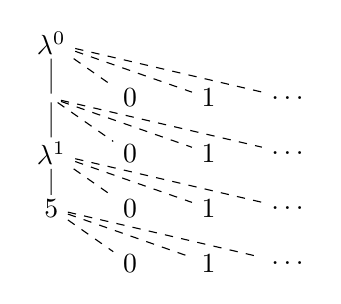
\begin{tikzpicture}[level distance=7mm,inner ysep=0.5mm,sibling distance=10mm]
\node {$\lambda^0$}
    child[missing]{}
    child[missing]{}
    child[missing]{}
    child {
        node {\pcfsucc}
        child[missing]{}
        child[missing]{}
        child[missing]{}
        child {
            node {$\lambda^1$}
            child[missing]{}
            child[missing]{}
            child[missing]{}
            child{
                node{$5$}
                child[missing]{}
                child[missing]{}
                child[missing]{}
                child[missing]{}
                child{node{$0$} edge from parent[dashed]}
                child{node{$1$} edge from parent[dashed]}
                child{node{$\ldots$} edge from parent[dashed]}
            }
            child{node{$0$} edge from parent[dashed]}
            child{node{$1$} edge from parent[dashed]}
            child{node{$\ldots$} edge from parent[dashed]}
        }
        child{node{$0$} edge from parent[dashed]}
        child{node{$1$} edge from parent[dashed]}
        child{node{$\ldots$} edge from parent[dashed]}
    }
    child{node{$0$} edge from parent[dashed]}
    child{node{$1$} edge from parent[dashed]}
    child{node{$\ldots$} edge from parent[dashed]}
;
\end{tikzpicture}
\end{center}

The following sequence of nodes is a traversal of $\tau(M)$:
$$ \Pstr[20pt]{ t = (l0){\lambda^0} \cdot (succ){\pcfsucc} \cdot (l1){\lambda^1} \cdot (c5){5} \cdot (v55-c5){5_5} \cdot (5l1-l1){5_{\lambda^1}} \cdot (6succ-succ){6_\pcfsucc} \cdot (6l0-l0,35){6_{\lambda^0}}}.
$$

The subsequences $t^*$ and $t \filter r$ are given by:
$$
\Pstr[17pt]{ t^* = (l0){\lambda^0} \cdot (l1-l0){\lambda^1} \cdot
(5l1-l1){5_{\lambda^1}} \cdot (6l0-l0){6_{\lambda^0}}.
\qquad  \mbox{ and } \qquad t
\filter r = (l0b){\lambda^0} \cdot
(6l0b-l0b){6_{\lambda^0}}. }
$$
We have $\varphi(t^*) = q_0 \cdot q_5 \cdot 5_{q_5} \cdot 5_{q_0}$
and $\varphi(t\filter r) = q_0 \cdot 5_{q_0}$ where $q_0$
and $q_5$ denote the roots of two flat arenas over $\nat$. These two
sequences of moves correspond to some play of the interaction
semantics and the standard semantics respectively. The interaction
play is represented below:
\begin{center}
\begin{tikzpicture}[style={anchor=base}]
\matrix (m) [matrix of math nodes]
{
\textbf{1} & \stackrel{5}{\longrightarrow} & \nat & \stackrel{\pcfsucc}{\longrightarrow} & \nat \\
&&&&  \node(q0){q_0}; \\
&&  \node(q5){q_5}; \\
&&  \node(a5){5_{q_5}}; \\
&&&&  \node(a6){6_{q_0}}; \\
};
\path (q5) edge[tableptr] (q0);
\draw[tableptr] (a5.west) .. controls +(160:0.2cm) and +(220:0.2cm) .. (q5.west);
\draw (a6) edge[tableptr] (q0);
\end{tikzpicture}
\end{center}

\subsubsection{Second example: the conditional operator}

\piccaption{The computation tree of the term $\lambda x y . \pcfcond\ 1\ x\ y$.}
\parpic[l]{
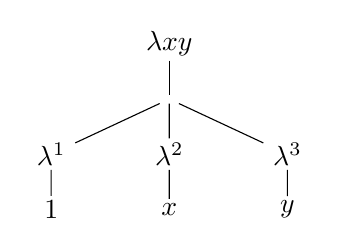
\begin{tikzpicture}[level distance=7mm,inner ysep=0.5mm,baseline=(root.base)]
\path
node (root) {$\lambda x y$}
child {
    node {\pcfcond}
    child {
        node {$\lambda^1$}
        child{
            node{$1$}
        }
    }
    child{
        node {$\lambda^2$}
        child{
            node{$x$}
        }
    }
    child{
        node {$\lambda^3$}
        child{
            node{$y$}
        }
    }
};
\end{tikzpicture}
}
Take the computation tree represented on the left (value-leaves are not shown). For any value $v \in\mathcal{D}$ the following sequence of nodes is a traversal:
$$\Pstr[27pt]{ t = (lxy){\lambda x y} \cdot (cond){\pcfcond} \cdot (l1-cond){\lambda^1} \cdot (1){1} \cdot (v11-1){1_1}
    \cdot (l3){\lambda^3} \cdot (y-lxy){y} \cdot (vy-y){v_y}  \cdot (vl3-l3){v_{\lambda^3}} \cdot (vcond-cond,30){v_{\pcfcond}}
    \cdot (vlxy-lxy,30){v_{\lambda x y}}.
}
$$
The subsequence $t^*$ and the reduction $t \filter\theroot$ are:
$$
\Pstr[17pt]{ t^* =  (lxy){\lambda x y} \cdot
        (l1-lxy){\lambda^1} \cdot
        (l3-lxy){\lambda^3} \cdot
        (y-lxy){y} \cdot
        (vy-y){v_y}  \cdot
        (vl3-l3){v_{\lambda^3}} \cdot
        (vlxy-lxy,35){v_{\lambda x y}}
\qquad  \mbox{ and } \qquad t \filter\theroot =
(lxyb){\lambda x y} \cdot (yb-lxyb){y} \cdot (vyb-yb){v_y}
\cdot (vlxyb-lxyb){v_{\lambda x y}}.
}
$$
The correspondence theorem tells us that the sequence of moves $\varphi(t^*)$ (represented in the diagram below) is a play of the
revealed semantics, and the sequence $\varphi(t\filter\theroot)$
is a play of the standard semantics that is obtained by hiding the internal moves from $\varphi(t^*)$.

\begin{center}
\begin{tikzpicture}[style={anchor=base}]
  \matrix[matrix of math nodes]
  {
  \nat & \times & \nat & \stackrel{\sigcol{\langle \sem{1}, \pi_1, \pi_2\rangle}}\longrightarrow & \nat & \times & \nat & \times &
\nat & \stackrel{\mucol\pcfcond}\longrightarrow & \nat \\
&&&&&&&&&&  \node(q0){q_0^{(\lambda x y)}}; \\
&&&&  \node(qa){q_a^{(\lambda^1)}}; \\
&&&&  \node(1){1}; \\
&&&&&&  \node(qb){q_b^{(\lambda^2)}}; \\
&&  \node(qy){q_y^{(y)}}; \\
&&  \node(vqy){v_{q_y}}; \\
&&&&&&  \node(vqb){v_{q_b}}; \\
&&&&&&&&&& \node(vq0){v_{q_0}}; \\
};
\path (vq0) edge[tableptr] (q0);
\path (vqb) edge[tableptr] (qb);
\draw[->] (vqy.west) .. controls +(160:0.2cm) and +(220:0.2cm) .. (qy.west);
\path (qy) edge[tableptr] (qb);
\path (qb) edge[tableptr] (q0);
\draw[->] (1.west) .. controls +(160:0.2cm) and +(200:0.2cm) .. (qa.west);
\path (qa) edge[tableptr] (q0);
\end{tikzpicture}
\end{center}


\subsection{Idealized algol}

We now consider the language Idealized Algol. The general idea is the same as for \pcf, however there are some difficulties caused by the presence of the two new
base types \iavar\ and \iacom. We just give indications on how to
adapt our framework to the particular case of \ialgol\ without
giving the complete proofs. However we believe that enough
indications are given to convince the reader that the argument used
in the \pcf\ case can be easily adapted to \ialgol.

\subsubsection{Computation hypertree}
Crucially, all the languages that we have considered up to now (lambda calculus and \pcf) do not have product types. Consequently, the arenas involved in their game model only have a single initial move at most, and therefore they can be
regarded as trees. This had permitted us to represent the game denotation of term directly on some representation of its abstract syntax tree. In \ialgol, however, the type \iavar\ is given by the product $\iacom^{\nat} \times \iaexp$. Therefore the corresponding game has an infinite number of initial moves. But tree structures such as the AST of the term have only one root therefore we have to find a different way to represent the game semantics.

The solution consists in using a hypertree representation instead of just a tree. This hypertree is an abstract graph representation of the syntax of the term in which some nodes, called \emph{generalized lambda nodes}, are themselves constituted of (possibly infinitely many) subnodes. Each subnode can be connected to different children nodes of the generalized node.


\emph{Notations:} For any type $\mu$, we write
$\mathcal{D}_\mu$ to denote the set of values of type $\mu$.
We have $\mathcal{D}_{\iaexp} = \nat$,
$\mathcal{D}_{\iacom} = \{ \iadone \}$
and $\mathcal{D}_{\iavar} = \mathcal{D}_{\iaexp} \union \mathcal{D}_{\iacom}$. For any node $n$, if $\kappa(n)$ is of type $(A_1,\ldots A_n,B)$, we call $B$ the \emph{return type of $n$}. The set of value-leaves of a node $n$ is given by $\mathcal{D}_{\mu}$ where $\mu$ is the return type of $n$.
For conciseness, when representing value-leaves in the DAG, we merge all the value-leaves of a given node of type $\mu$ into a single leaf labelled $\mathcal{D}_\mu$.

For instance the tree
\begin{center}
\begin{tikzpicture}[level distance=7mm,inner ysep=0.5mm,baseline=(root.base),sibling distance=5mm]
\path
node (root) {$n$}
child {
    node {$\mathcal{D}_\iaexp$}
}
+(1.5,0) node {stands for}
+(3,0)
node {$n$}
    child {node {$0$} }
    child {node {$1$}}
    child {node {$2$}}
    child {node {$\ldots$}}
+(7,0) node {and}
+(8,0)
node {$n$}
child{
    node{$\mathcal{D}_\iacom$}
}
+(9,0) node {for}
+(10,0)
node {$n$}
child{
    node{\iadone}
};
\end{tikzpicture}.
\end{center}

The computation hypertree of a term of type \iavar has infinitely many root $\lambda$-nodes which are merged all-together into a single node called a \defname{generalized lambda-node}. Nodes with return type \iavar have a generalized lambda node as parent.
The subnodes of a generalized lambda nodes are labelled
$\lambda^r$, $\lambda^{w_0}$, $\lambda^{w_1}$, $\lambda^{w_2}$, \ldots
Suppose that $M$ is a term of type \iavar, then the computation hypertree for $\lambda \overline{\xi} . M$ is obtained by relabelling the root $\lambda$-nodes $\lambda^r$,
$\lambda^{w_0}$, $\lambda^{w_1}$, $\lambda^{w_2}$, \ldots into
$\lambda^r \overline{\xi}$, $\lambda^{w_0} \overline{\xi}$,
$\lambda^{w_1} \overline{\xi}$, $\lambda^{w_2} \overline{\xi}$,
\ldots. For a term $M$  of type \iaexp\ or \iacom, the computation
hypertree for $\lambda \overline{\xi} . M$ is computed as defined previously for computation trees in the $\lambda$-calculus.

Table \ref{tab:ia_computationdag} shows the computation hypertree for each term-construct of \ialgol. The generalized lambda nodes are circled (line 2 and 6).

\notetoself{circle the gener. lambda nodes}

\begin{table}
\begin{center}
\begin{tabular}{lc}
$M$ & $\tau(M)$ \\ \hline \hline \\
\parbox{3cm}{x $: \mu$ \\
$\mu \in \{ \iacom, \iaexp \}$} &

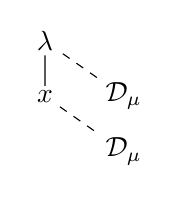
\begin{tikzpicture}[level distance=7mm,inner ysep=0.5mm,sibling distance=10mm]
\node {$\lambda$}
child[missing]{}
child {
    node {$x$}
    child[missing]{}
    child[missing]{}
    child {
        node {$\mathcal{D}_\mu$}
        edge from parent[dashed]
    }
}
child{node{$\mathcal{D}_\mu$} edge from parent[dashed]}
;
\end{tikzpicture}
\\ \\
x : \iavar &
\begin{tikzpicture}
\matrix (m) [matrix of math nodes, row sep=5mm]
{
\lambda^r & \lambda^{w_0} & \lambda^{w_1}  & \lambda^{w_2} & \lambda^{w_{\ldots}} \\
    \mathcal{D}_\iaexp &  & x & & \iadone \\
    &  &  & \mathcal{D}_\iaexp & \iadone \\
};
\draw[-] (m-1-1) -- (m-2-3)
         (m-1-2) -- (m-2-3)
         (m-1-3) -- (m-2-3)
         (m-1-4) -- (m-2-3)
         (m-1-5) -- (m-2-3);
\draw[dashed] (m-2-3) -- (m-3-4)
              (m-2-3) -- (m-3-5)
              (m-1-1) -- (m-2-1)
              (m-1-5) -- (m-2-5)
              (m-1-4) -- (m-2-5)
              (m-1-3) -- (m-2-5)
              (m-1-2) -- (m-2-5);
\end{tikzpicture}
\\ \\
\iaskip : \iacom &
    \begin{tikzpicture}[level distance=7mm,inner ysep=0.5mm,sibling distance=10mm]
\node {$\lambda$}
child[missing]{}
child {
    node {\iaskip}
    child[missing]{}
    child[missing]{}
    child {
        node {\iadone}
        edge from parent[dashed]
    }
}
child{node{\iadone} edge from parent[dashed]}
;
\end{tikzpicture}
\\ \\
$\iaassign\ L\ N :\iacom$ &
\begin{tikzpicture}[level distance=7mm,inner ysep=0.5mm,sibling distance=20mm]
\node {$\lambda$}
child[missing]{}
child {
    node {\iaassign}
    child{node{$\tau(N:\iaexp)$}}
    child{node{$\tau(L:\iavar)$}}
    child {
        node {\iadone}
        edge from parent[dashed]
    }
}
child{node{\iadone} edge from parent[dashed]};
\end{tikzpicture}
\\ \\
$\iaderef\ L :\iaexp$ &
\begin{tikzpicture}[level distance=7mm,inner ysep=0.5mm,sibling distance=15mm]
\node {$\lambda$}
child[missing]{}
child {
    node {\iaderef}
    child[missing]{}
    child{node{$\tau(L:\iavar)$}}
    child {
        node {\iadone}
        edge from parent[dashed]
    }
}
child{node{\iadone} edge from parent[dashed]}
;
\end{tikzpicture}
\\ \\
\parbox{3cm}{$\iaseq_{\mu}\ N_1\ N_2 :\iacom$\\ $\mu\in\{\iaexp,\iacom\}$} &
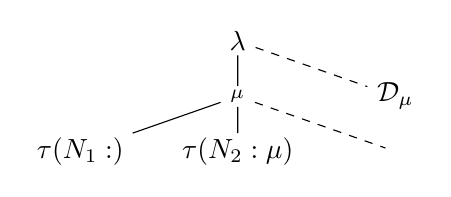
\begin{tikzpicture}[level distance=7mm,inner ysep=0.5mm,sibling distance=20mm]
\node {$\lambda$}
child[missing]{}
child {
    node {$\iaseq_\mu$}
    child{node{$\tau(N_1:\iacom)$}}
    child{node{$\tau(N_2:\mu)$}}
    child { node {\iadone} edge from parent[dashed] }
}
child{node{$\mathcal{D}_\mu$} edge from parent[dashed]};
\end{tikzpicture}
\\ \\
$\iamkvar\ N_w\ N_r :\iavar$ &
\begin{tikzpicture}
\matrix (m) [matrix of math nodes, row sep=5mm]
{
  \lambda^r & \lambda^{w_0} & \lambda^{w_1}  & \lambda^{w_2} & \lambda^{w_{\ldots}} \\
    \mathcal{D}_\iaexp &  & \iamkvar & & \iadone \\
    & \tau(N_r) & \tau(N_w) & \mathcal{D}_\iaexp & \iadone \\
};
\draw[-] (m-1-1) -- (m-2-3)
         (m-1-2) -- (m-2-3)
         (m-1-3) -- (m-2-3)
         (m-1-4) -- (m-2-3)
         (m-1-5) -- (m-2-3)
         (m-2-3) -- (m-3-2)
         (m-2-3) -- (m-3-3);
\draw[dashed] (m-2-3) -- (m-3-4)
              (m-2-3) -- (m-3-5)
              (m-1-1) -- (m-2-1)
              (m-1-5) -- (m-2-5)
              (m-1-4) -- (m-2-5)
              (m-1-3) -- (m-2-5)
              (m-1-2) -- (m-2-5);
\end{tikzpicture}
\\ \\
\parbox{3cm}{$\ianewin{x}\ N : \mu$ \\ $\mu \in \{ \iacom, \iaexp \} $} &
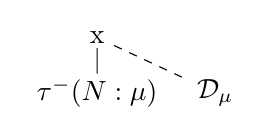
\begin{tikzpicture}[level distance=7mm,inner ysep=0.5mm,sibling distance=15mm]
\node {\ianewin{x}}
child[missing]{}
child{node{$\tau^-(N:\mu)$}}
child { node {$\mathcal{D}_\mu$} edge from parent[dashed]};
\end{tikzpicture}
\end{tabular}
\bigskip

where $\tau^-(N)$ denotes the DAG obtained by removing the root nodes from $\tau^-(N)$.
\end{center}
  \caption{Computation DAGs for the constructs of \ialgol.}
  \label{tab:ia_computationdag}
\end{table}

In a computation hypertree, the parent of a generalized lambda nodes shares an edge with each of the lambda node inside the generalized lambda node. Therefore in Table \ref{tab:ia_computationdag},

... stands for ...

\notetoself{ typset the corresponding trees}


\emph{Notation:} Let $p$ be a node and suppose that its $i$th child $n$ has the
return type \iavar. Then $n$ is a generalized lambda-node with subnodes
$\lambda^r \overline{\xi}$, $\lambda^{w_0}
\overline{\xi}$, \ldots. From the point of view of the parent node $p$, these nodes are referenced as ``$i.\alpha$'' where $i\in\{0..arity(p)\}$ and $\alpha \in \{ r\} \union\{ w_k \ | \ k \in \nat \}$. For instance  $i.r$ refers to the root labelled $\lambda^r \overline{\xi}$ of the $i$th child of $p$, and
$i.w_k$ refers to the root labelled $\lambda^{w_k} \overline{\xi}$.




\subsubsection{Traversals}


\begin{itemize}
\item \emph{The application rule}

There are two rules (app$_{\iaexp}$) and (app$_{\iacom}$)
corresponding to traversals ending with an @-node of return type
\iaexp\ and \iacom\ respectively. These rules are identical to the
rule \iaexp\ of section \ref{subsec:traversal}.

The application rule for $@$-nodes with return type \iavar\ is:
$$\rulename{app_\iavar}
\rulef{ \Pstr{t \cdot (lHyp){\lambda^k \overline{\xi}} \cdot
(appHyp-lHyp,35:0){@} \in \travset }
 }{\Pstr[18pt] {t \cdot (l){\lambda^k
\overline{\xi}} \cdot (app-l,35:0){@} \cdot (l2-app,35:0.k){\lambda^k
\overline{\eta}} \in \travset }}
 \ k \in \{ r, w_0, w_1, \ldots \}
$$


\item \emph{Input-variable rules}

There are two rules \rulenamet{InputVar^\iaexp} and \rulenamet{InputVar^\iacom}
which are the counterparts of rule \rulenamet{InputVar} of section
\ref{subsec:traversal} and are defined identically.

Let $x$ be an input-variable of type \iavar.
$$ \rulename{InputVar^\iavar_r}
\rulef{t \cdot \lambda^r \overline{\xi} \cdot x \in \travset \qquad v\in\mathcal{D} }
    {t \cdot \lambda^r \overline{\xi} \cdot x \cdot v_x \in \travset}
\hspace{1.5cm} \rulename{InputVar^\iavar_w} \rulef{t \cdot
\lambda^{w_i} \overline{\xi} \cdot x \in \travset}
    {t \cdot \lambda^{w_i} \overline{\xi} \cdot x \cdot \iadone_x \in \travset }
$$

\item \emph{IA constants rules}

Table \ref{tab:ia_travrules} gives the traversal rules corresponding to the interpreted constants of \ialgol.
The rules for \ianew\ are purely structural, they are defined the
same way as the rules \rulenamet{app_\iaexp}, \rulenamet{app_\iacom} and
\rulenamet{app_\iadone}.

\begin{table}[htbp]
$$
\begin{array}{ll}
\rulename{deref} \rulef{t \cdot \iaderef \in \travset}{\Pstr[15pt]{t \cdot (d){\iaderef} \cdot (n-d,35:1.r){n} \in \travset }}
&
\rulename{deref'}
\rulef{t \cdot \iaderef \cdot n \cdot t_2 \cdot v_n \in \travset} {t
\cdot \iaderef \cdot n \cdot t_2 \cdot v_n \cdot v_{\iaderef}\in
\travset }
\\[30pt]
\rulename{assign} \rulef{t \cdot \iaassign \in \travset}{\Pstr[16pt]{t \cdot (ass){\iaassign} \cdot (n-ass,35:1){\lambda} \in \travset} }
&
\rulename{assign'}
\rulef{\Pstr{t \cdot \iaassign \cdot (n)\lambda \cdot t_2 \cdot (vn-n){v_\lambda}} \in
\travset} {\Pstr[25pt]{t \cdot (ass){\iaassign} \cdot (n){\lambda} \cdot
t_2 \cdot (vn-n){v_\lambda} \cdot (m-ass,35:2.w_n){\lambda\overline\eta} \in \travset } }
\\[40pt]
\multicolumn{2}{l}{\rulename{assign''}  \rulef{\Pstr[1.7cm]{t \cdot (assHyp){\iaassign} \cdot t_2 \cdot (mHyp-assHyp,35:2.w_k){\lambda\overline\eta} \cdot t_3 \cdot (vmHyp-mHyp){\iadone_{\lambda\overline\eta}} \in \travset}}
{\Pstr[0.7cm]{t \cdot (ass)\iaassign \cdot t_2 \cdot (m){\lambda\overline\eta} \cdot t_3 \cdot (vm-m,25){\iadone_{\lambda\overline\eta}} \cdot
(vass-ass,20){\iadone_\iaassign} \in \travset} }
}
\\[30pt]
\rulename{seq} \rulef{t \cdot \iaseq \in \travset}{\Pstr[13pt]{t \cdot (seq){\iaseq} \cdot (n-seq,35:1){n} \in \travset } }
&
\rulename{seq'}
\rulef{t \cdot \iaseq \cdot n \cdot t_2 \cdot v_n \in
\travset} {\Pstr[18pt]{ t \cdot (seq){\iaseq} \cdot (n){n} \cdot t_2
\cdot v_n \cdot (m-seq,25:2){m} \in \travset }}
\\[30pt]
\multicolumn{2}{l}{\rulename{seq''} \rulef{\Pstr{t \cdot (seqHyp){\iaseq} \cdot t_2 \cdot (mHyp-seqHyp,35:2){m} \cdot t_3 \cdot v_m \in \travset}}
{t \cdot \iaseq \cdot t_2 \cdot m \cdot t_3 \cdot v_m \cdot
v_{\iaseq} \in \travset }}
\\[30pt]
\rulename{mkvar_r} \rulef{t \cdot \lambda^r \overline{\xi} \cdot \iamkvar \in \travset}{\Pstr[14pt]{t \cdot \lambda^r \overline{\xi} \cdot (d){\iamkvar} \cdot (n-d,35:1){\lambda} \in \travset} }
&\rulename{mkvar_r'}
\rulef{\Pstr{t \cdot \iamkvar \cdot (n)\lambda \cdot t_2 \cdot (vn-n){v_\lambda} \in \travset}} {\Pstr[17pt]{t \cdot (mk)\iamkvar \cdot (n)\lambda \cdot t_2 \cdot (vn-n){v_\lambda} \cdot (vmk-mk,25){v_{\iamkvar}}\in
\travset}}
\\[30pt]
\rulename{mkvar_w} \rulef{t \cdot \lambda^{w_k} \overline{\xi} \cdot \iamkvar \in \travset}{\Pstr[15pt]{t \cdot \lambda^{w_k} \overline{\xi} \cdot (mk){\iamkvar} \cdot (n-mk,35:2){\lambda\overline\eta} \in \travset} }
%\\[30pt] \multicolumn{2}{l}
&
{\rulename{mkvar_w''}  \rulef{\Pstr[25pt]{t \cdot \lambda^{w_k} \overline{\xi} \cdot \iamkvar \cdot (n){\lambda\overline\eta} \cdot t_2 \cdot (vn-n,25){\iadone_{\lambda\overline\eta}} \in \travset}}
{\Pstr[17pt]{t \cdot \lambda^{w_k} \overline{\xi} \cdot (mk)\iamkvar \cdot (n){\lambda\overline\eta} \cdot
t_2 \cdot (vn-n,25){\iadone_{\lambda\overline\eta}} \cdot (vmk-mk,20)\iadone_{\iamkvar} \in \travset}}
}
\end{array}
$$
where $v$ denotes some value from $\mathcal{D}$.
\caption{Traversal rules for \ialgol\ constants}
\label{tab:ia_travrules}
\end{table}


The four rules given in Table \ref{tab:ia_travrules} are not sufficient to model the constant \iamkvar.
Indeed, consider the term $\iaassign\ (\iamkvar\ (\lambda x . M) N)
7$. The rule (\mbox{mkvar}$_w''$) permits to traverse the node
\iamkvar\ and to go on by traversing the computation tree of
$\lambda x . M$. The problem is that when traversing $\tau(M)$, if
we reach a variable $x$, we are not able to relate $x$ to the value
$7$ that is assigned to the variable.

To overcome this problem, we need to define traversal rules for
variable in such a way that a variable node bound by the second
child of a $\iamkvar$-node is treated differently from other
variables.

\item \emph{Variable rules}
Let $x$ be an internal variable node \ie either hereditarily justified by an @-node or by a $\Sigma$-constant node. There are two cases depending on whether $x$ is a $\lambda$-abstracted variable or a block-allocated variable declared with a ``$\ianewin{x}$'' construct.

\begin{itemize}
\item Suppose that $x$'s binder is a lambda-node $\lambda \overline{x}$ and $x \in N^{@\vdash}$.

Then this occurrence of $x$ corresponds to an internal variable of type \iavar\ which would be substituted by another term if the term were to be reduced to normal form. This case is treated a generalization of the case treated by rule \rulenamet{Var} (see Sec.\ \ref{subsec:traversal}) to variables of type \iavar. This generalization is straightforward: the lambda nodes preceding $x$ in the traversals determines which lambda-nodes will be visited next:
$$ \rulename{Var_\iavar}
    \rulef{\Pstr[0.5cm]{t \cdot (n){n} \cdot (lx){\lambda \overline{x}}     \ldots \lambda^\alpha x_i \cdot (x-lx,50:i){x_i} } \in \travset \quad x_i \in N_{\sf var}^{@\vdash}}
{\Pstr[23pt]{t \cdot (n){n} \cdot (lx){\lambda \overline{x}}
\ldots \lambda^\alpha x_i \cdot  (x-lx,30:i){x_i} \cdot (letai-n,40:i.\alpha){\lambda\overline{\eta_i}}
\in \travset \raisebox{0pt}[25pt]{}}}
$$
where $\alpha$ belongs to $\{r\} \union \{w_i \ | \ i \in \nat \}$.

\item Suppose that $x$'s binder is a lambda-node and $x \in N^{N_\Sigma\vdash}$.

In \ialgol, the only $\Sigma$-constant node of order greater than 1 is \iamkvar, therefore a lambda-node that is hereditarily enabled by a $\Sigma$-node is necessarily the second child of a \iamkvar-node.
Hence $x$'s binder is a lambda node labelled $\lambda x$
and is the second child of a \iamkvar-node. This case is handled by the following rule:
$$ \rulename{\iamkvar\mbox{-}Var}  \rulef{\Pstr[17pt]{t \cdot \lambda^{w_k} \overline{\xi} \cdot \iamkvar \cdot (lx)\lambda x \cdot t_2 \cdot (x-lx)x \in \travset}}
{\Pstr[15pt]{t \cdot \lambda^{w_k}\overline{\xi} \cdot \iamkvar \cdot (lx)\lambda x \cdot t_2 \cdot (x-lx)x \cdot (kx-x)k_x \in \travset }}
$$

\item Suppose that $x$ is block-allocated with $\ianewin{x}$.

In a justified sequence of nodes of the form
$\Pstr[17pt]{(decl){\ianewin{x}}\cdot \ldots \cdot \lambda^{w_k}\overline\xi \cdot (x-decl,25){x}}$ for some $k\in \mathcal{D}_{\iaexp}$, the segment  $\lambda^{w_k}\overline\xi \cdot x$ is called an \defname{assignment of $x$ with respect to (the occurrence of)  the node ``\ianewin{x}''}. We have the following rules:
$$
\begin{array}{lll}
\rulename{\ianew\mbox{-}Var_w}
&
    \rulef{
        t \cdot \lambda^{w_k} \overline{\xi} \cdot x \in \travset
        \quad x \in N^{\ianew\vdash}_{\sf var}
    }
    {   t \cdot \lambda^{w_k} \overline{\xi} \cdot x \cdot \iadone_x \in
        \travset
    },
\\[20pt]
\rulename{\ianew\mbox{-}Var_r}
&
    \rulef{
        \Pstr[17pt]{t_1 \cdot (decl){\ianewin{x}} \cdot t_2 \cdot \lambda^r \overline{\xi} \cdot (x-decl,25){x} \in \travset}
    }
    {   t_1 \cdot \ianewin{x} \cdot t_2 \cdot \lambda^r \overline{\xi}
        \cdot x \cdot 0_x \in \travset
    }
&    \parbox{4cm}{if $t_2$ contains no assignment of $x$;}
\\[20pt]
\rulename{\ianew\mbox{-}Var'_r}
&    \rulef{
        \Pstr[15pt]{
            t_1 \cdot (decl){\ianewin{x}} \cdot t_2 \cdot \lambda^r \overline{\xi} \cdot (x-decl,25){x} \in \travset
        }
    }
    {
        t_1 \cdot \ianewin{x} \cdot t_2 \cdot \lambda^r \overline{\xi} \cdot x \cdot k_x \in \travset
    }
&    \parbox{4cm}{if the last assignment of $x$ in $t_2$ is
of the form $\lambda^{w_k} \cdot x$ for some $k\in\nat$.}
\end{array}$$
\end{itemize}
\end{itemize}

\subsubsection{Game semantics correspondence}
The properties that we proved for computation trees and traversals
of the $\lambda$-calculus with constants can easily be lifted
to computation hypertrees of \ialgol. In particular:
\begin{itemize}
\item constant traversal rules are well-behaved (for order-$0$ and order-$1$ constants, this is a consequence
of Lemma \ref{lem:sigma_order1_are_wellbehaved}; for $\iamkvar$
however it needs to be proved separately);
\item P-view of traversals are paths in the computation hypertrees;
\item the P-view of the reduction of a traversal is the reduction of the P-view,
and the O-view of a traversal is the O-view of its reduction
(Lemma \ref{lem:pview_trav_projection} and
\ref{lem:oview_trav_projection});
\item there is a mapping from vertices of the computation hypertrees to moves in the interaction game semantics;
\item there is a correspondence between traversals of the computation tree and plays in interaction game semantics;
\item consequently, there is a correspondence between the standard game semantics and
the set of justified sequences of nodes $\travset(M)^{\filter
\theroot}$.
\end{itemize}


    \section{Related works and conclusion}
    \input{corresp_conclusion.texi}
\fi


\chapter{Syntactic analysis of the game denotation of safe terms}
    \label{chap:syntactic_gamesem}
    \notetoself{This chapter is taken from my transfer report. I need to
rework it to integrate it correctly within the present thesis.}


Safety has been defined as a syntactical constraint. Since Game
Semantics is by essence syntax-independent, it seems difficult at
first sight to give a game-semantic characterization of a syntactic restriction such as the Safety Condition.
In fact, the Correspondence Theorem makes such analysis possible since it allows us to regard the plays of a strategy
as sequences of nodes of some AST of the term.


The main theorem of this chapter (theorem
\ref{thm:safe_ptr_recoverable}) states that pointers in a play of
the strategy denotation of a safe term can be uniquely recovered
from O-questions' pointers and from the underlying sequence of
moves. The proof is in several steps. We start by introducing the
notion of \emph{P-incrementally-justified strategies} and prove that
for plays of such strategies, pointers emanating from P-moves can be
reconstructed uniquely from the underlying sequences of moves and
from O-moves' pointers. We then introduce the notion of
\emph{incrementally-bound computation trees} and prove that
incremental-binding coincides with P-incremental-justification
(proposition \ref{prop:Nher_incrbound_iff_incrjustified}).


Finally, we show that safe simply-typed terms in $\beta$-normal form
have incrementally\--bound computation trees, consequently their
game denotation is P-incrementally-justified.


The first section of this chapter is concerned only with the safe $\lambda$-calculus without interpreted constants. In the next
section we extend the result by taking into account the interpreted
constants of \pcf\ and \ialgol. We define the language safe \ialgol\
(resp. safe \pcf) to be the fragment of \ialgol\ (resp. \pcf) where
the application and abstraction rules are constrained the same way
as in the safe $\lambda$-calculus. We show that safe \pcf\ terms are
denoted by P-incrementally-justified strategies and we give the key
elements for a possible extension of the result to Safe Idealized
Algol.

\section{Preliminaries}

In this section, we assume that we work in a general setting of a
language extending the simply-typed lambda calculus with new
constants and respecting the following prerequisites:
\begin{itemize}
\item A fully-abstract game-semantic model of the language is
defined;
\item A notion of safety is defined for the language such that the
restriction of the language to the safe pure simply-typed
fragment coincides with the definition of the Safe Lambda
Calculus and such that for any typable term $\Gamma \vdash M :
T$ we have $\forall z \in \Gamma . \ord{z} \geq \ord{T}$ ;
\item The small-step reduction semantics of the language preserves safety;
%\item Substitution preserves safety.
\item New traversal rules are defined to take into account the constants of the language.
\item Constant traversal rules are well-behaved (see Def.\
\ref{def:wellbehaved_traversal});
\item Constant traversal rules correctly model the behaviour of the constants in such a way
that the game-semantic correspondence (Theorem
\ref{thm:correspondence}) still holds.
\end{itemize}

The simply-typed lambda calculus is of course such a language, but
we will show that \pcf\ also lends itself into this setting.

For the rest of this section we fix a term $\Gamma \vdash M : T$
from this generic language. We will explicitly specify when a result
holds only in the pure (\ie no constants) simply-typed calculus
fragment of the language.

\subsection{Incremental binding}

In a computation tree, a binder node always occurs in the path from
the bound node to the root. We now introduce a class of computation
trees in which binder nodes can be uniquely recovered from the order
of the nodes. We call path any sequence of nodes such that for any
two consecutive nodes $a \cdot b$ in the sequence, $a$ is the parent
of $b$. We write $[n_1,n_2]$ to denote the path going from node
$n_1$ to node $n_2$ equipped with the justification pointers induced
by the enabling relation $\vdash$ (each node of the tree has a
unique enabler in the path to the root thus for each occurrence in
$[n_1,n_2]$ there is at most one occurrence of its enabler in
$[n_1,n_2]$). We write $]n_1,n_2]$ for the sub-sequence of
$[n_1,n_2]$ obtained by removing $n_1$ as welle as all the
associated pointers.

We recall that $\theroot$ denotes the root of the computation tree
$\tau(M)$ and $N^{\theroot\vdash}$ denotes the subset of $N$
consisting of nodes that are hereditarily enabled by $\theroot$.



\begin{definition}[Incrementally-bound computation tree]
Let $A$ be a subset of nodes of the computation tree. A variable
node $x$ of a computation tree is said to be
\defname{$A$-incrementally-bound} if its enabler is the first
$\lambda$-node from $A$ in the path to the root that has order
strictly greater than $\ord{x}$. Formally:
\begin{align*}
x \mbox{ is $A$-incrementally-bound} \  \iff \  \left\{
                                                  \begin{array}{ll}
                                                    x \hbox{ is enabled by } b \in [\theroot,x]\inter A \ ; \\
                                                    \ord{b} > \ord{x} \;\\
                                                    \forall \lambda\mbox{-node } n' \in ]n,x]\inter A  . \ord{n'} \leq \ord{x} \ .
                                                  \end{array}
                                                \right.
\end{align*}

This definition can be split into two cases:
\begin{enumerate}
\item $x$ is \emph{bound} by the first $\lambda$-node from $A$ occurring in the path to the root that has
order strictly greater than $\ord{x}$.
\item or $x$ is a \emph{free variable} and all the $\lambda$-nodes from from $A$ occurring in the path to the root except the root have order
 smaller or equal to $\ord{x}$.
\end{enumerate}

A computation tree is said to be \defname{$A$-incrementally-bound},
also abbreviated $A$-i.b., if all the variable nodes from $A$ are
$A$-incrementally-bound.

We say that a node (resp.\ a tree) is
\defname{incrementally-bound} if it is
\defname{$N$-incrementally-bound} where $N$ is the entire set of nodes of the computation tree.
\end{definition}

Clearly for any two sets of nodes $A$ and $B$ verifying $A\subseteq
B$ we have that $B$-incremental-binding implies
$A$-incremental-binding.


\smallskip

Let $\closure{M}$ denote the function that converts $M$ into the
closed term obtained from $M$ by abstracting all its free variables
(in order of appearance in the term). From the previous definition,
if $\tau(M)$ is $A$-i.b.\ then so is $\tau(\closure{M})$.

\smallskip

A node of the computation tree is said to be \defname{reachable} if
there is some traversal of the computation tree that visits it.


\begin{lemma}[Safe terms have incrementally-bound computation trees]
\label{lem:incrbound_iff_etanf_safe} Suppose that  $\Gamma \vdash M
:T$ is a simply-typed term.
\begin{itemize}
\item[(i)] If $M$ is a safe term then $\tau(M)$ is incrementally-bound ;
\item[(ii)] conversely, if $M$ is \emph{closed} and $\tau(M)$ is i.b.\ then the $\eta$-long normal form of $M$ is safe.
\end{itemize}
\end{lemma}
\begin{proof}
(i) Suppose that $M$ is safe. The safety property is preserved after
taking the $\eta$-long normal form, therefore $\tau(M)$ is the tree
representation of a safe term.

In the safe $\lambda$-calculus, the variables in the context with
the the lowest order must be all abstracted at once when using the
abstraction rule. Since the computation tree merges consecutive
abstractions into a single node, any variable $x$ occurring free in
the subtree rooted at a $\lambda$-node $\lambda \overline{\xi}$
different from the root must have order greater or equal to
$\ord{\lambda \overline{\xi}}$. Reciprocally, if a lambda node
$\lambda \overline{\xi}$ binds a variable node $x$ then
$\ord{\lambda \overline{\xi}} = 1+\max_{z\in\overline{\xi}} \ord{z}
> \ord{x}$.

Let $x$ be a bound variable node. Its binder occurs in the path from
$x$ to the root, therefore, according to the previous observation,
$x$ must be bound by the first $\lambda$-node occurring in $[r,x]$
with order strictly greater than $\ord{x}$. Let $x$ be a free
variable node then $x$ is not bound by any of the $\lambda$-nodes
occurring in $[\theroot,x]$. Once again, by the previous
observation, all these $\lambda$-nodes except $\theroot$ have order
smaller than $\ord{x}$. Hence $\tau$ is incrementally-bound.

(ii) Let $M$ be a closed term such that $\tau(M)$ is
incrementally-bound. We assume that $M$ is already in $\eta$-normal
form. We prove that $M$ is safe by induction on its structure. The
base case $M = \lambda \overline{\xi} . \alpha$ for some variable or
constant $\alpha$ is trivial. \emph{Step case:} If $M = \lambda
\overline{\xi} . N_1 \ldots N_p$. Let $i$ range over $1..p$. $N_i$
can be written $\lambda \overline{\eta_i} . N'_i$ where $N'_i$ is
not an abstraction. By the induction hypothesis, $\lambda
\overline{\xi} . N_i = \lambda \overline{\xi} \overline{\eta_i} .
N'_i$ is safe. Hence $\vdash \lambda \overline{\xi}
\overline{\eta_i} . N'_i$ is a valid judgment of safe
$\lambda$-calculus. But this judgment can only be derived using the
\rulenamet{Abs} rule on the term $N'_i$. Hence $N'_i$ is necessarily
safe. Let $z$ be a variable occurring free in $N'_i$. Since $M$ is
closed, $z$ is either bound by $\lambda \overline{\eta_1}$ or
$\lambda \overline{\xi}$. In the latter case, since $\tau(M)$ is
i.b., $\ord{z}$ is smaller than $\ord{\lambda
\overline{\eta_1}}=\ord{N_i}$ thus in both case we are allowed to
abstract the variables $\overline{\eta_1}$ using the rule
\rulenamet{Abs}. This shows that $N_i$ is safe.

Each of the $N_i$s is safe and $N_1 \ldots N_p$ is of type $o$
therefore by the rule \rulenamet{App} rule we have $\overline{\xi}
\vdash N_1 \ldots N_p$. Finally, \rulenamet{Abs} gives us the
judgement $\vdash M = \lambda \overline{\xi} . N_1 \ldots N_p$.
\end{proof}

Note that the hypothesis that $M$ is closed in (ii) is necessary.
For instance, the two terms $\lambda x y .x$ and $\lambda y . x$,
where $x,y:o$, have (isomorphic) incrementally-bound computation
trees. However $\lambda x y .x$ is safe whereas $\lambda y . x$ is
not.

\begin{corollary}
\label{cor:betared_preserve_incrbound} Suppose $M$ is a closed term
in $\eta$-long normal form. If $\tau(M)$ is incrementally-bound and
$M \betared N$ then $\tau(N)$ is incrementally-bound.
\end{corollary}
\proof Suppose that $\tau(M)$ is i.b. Then by Lemma
\ref{lem:incrbound_iff_etanf_safe}(ii), $M$ is safe and since safety
is preserved by $\beta$-reduction, so is $N$. Thus by Lemma
\ref{lem:incrbound_iff_etanf_safe}(i), $\tau(N)$ is
incrementally-bound. \qed
\smallskip

Note that this corollary  cannot be generalized to
$A$-incremental-binding for any set of node $A$. Take for instance
the eta-normal term $M = \lambda u^{o} v^{((o,o),o)} . (\lambda x^o
. v (\lambda z^o . x)) u$ which beta-reduces to $N = \lambda u v . v
(\lambda z . u)$. The computation trees are:
$$\pssetcomptree
\tau(M) = \pstree{\TR{\underline{\lambda u v}}}{\pstree{\TR{@}}{\pstree{\TR{\lambda
x}}{\pstree{\TR{\underline{v}}}{\pstree{\TR{\underline{\lambda
z}}}{\TR{x}}}}\pstree{\TR{\lambda }}{\TR{\underline{u}}}}} \hspace{2cm}
\tau(N) = \pstree{\TR{\underline{\lambda u v}}}{\pstree{\TR{\underline{v}}}{\pstree{\TR{\underline{\lambda z}}}{\TR{\underline{u}}}}}
$$
Take $A$ to be the set of nodes that are hereditarily justified by
the root (the nodes underlined in the above figure). Then $\tau(M)$
is $A$-incrementally-bound but $\tau(N)$ is not.


\subsection{P-incremental-justified strategies}
\begin{definition}[P-incremental-justification]
A strategy $\sigma$ on a game $A$ is
\emph{P-incrementally\-justified} if and only if for any sequence of
moves $s q \in P_A$ we have:
\begin{eqnarray*}
s q \in \sigma \wedge q \mbox{ is a P-question } &\implies&
\parbox[t]{9cm}{$q$  points to the last O-move in $\pview{s}$
with order strictly greater than $\ord{q}$.}
\end{eqnarray*}
\end{definition}




\begin{lemma}
\label{lem:incrjustified_pointers_uniqu_recover} Pointers emanating
from P-moves are superfluous for P-incrementally-justified
strategies.
\end{lemma}
\begin{proof}
Suppose $\sigma$ is a P-incrementally-justified strategy. We prove
that pointers attached to P-moves in a play $s\in \sigma$ are
uniquely recoverable by induction on the length of $s$. \noindent
\emph{Base case}: if $|s| \leq 1$ then there is no pointer to
recover. \noindent \emph{Step case}: suppose $s m \in \sigma$. If
$m$ is an answer move then by the well-bracketing condition $m$
points to the last unanswered question in $s$. If $m$ is a
P-question then by  P-incremental-justification of $\sigma$, $m$
points to the last O-move in $\pview{s}$ with order strictly greater
than $\ord{q}$. Since we have access to O-moves' pointers, we can
compute the P-view $\pview{s}$. Hence $m$'s pointer is uniquely
recoverable.
\end{proof}

%\begin{example}
%The denotation of the evaluation map $ev$ is
%P-incrementally-justified since it is the uncurrying of the identity
% map on the game A=>B.
%\end{example}



\begin{proposition}[Incremental-binding and P-incremental-justification]
\hfill

 \label{prop:Nher_incrbound_iff_incrjustified}

\begin{enumerate}[(i)]
\item Suppose $M$ is $\beta$-normal. Then if all the \emph{reachable} input-variable nodes of the computation tree
$\tau(\Gamma \vdash M : T)$ are
$N^{\theroot\vdash}$-incrementally-bound then $\sem{\Gamma
\vdash M : T}$ is P-incrementally-justified.

\item If $\sem{\Gamma \vdash M : T}$ is
P-incrementally-justified then all the \emph{reachable}
input-variable nodes of the computation tree $\tau(\Gamma \vdash
M : T)$ are $N^{\theroot\vdash}$-incrementally-bound.
\end{enumerate}
\end{proposition}

\begin{proof}
\noindent (i) Suppose that $\tau(M)$ is
$N^{\theroot\vdash}$-incrementally-bound, then so is
$\tau(\etalnf{\closure{M}})$. Thus by Corollary
\ref{cor:betared_preserve_incrbound} $\etalnf{\closure{M}}$ is safe
and since safety is preserved by $\beta$-reduction, so is its
beta-normal form. Thus by Lemma
\ref{lem:incrbound_iff_etanf_safe}(i),
$\tau(\betanf{\etalnf{\closure{M}}})$ is incrementally-bound. Hence
we can assume without loss of generality that $M$ is a closed term
in beta-normal form and prove that $\sem{M}$ is
P-incrementally-justified (This will imply that
$\sem{\betanf{\etalnf{\closure{M}}}}$ is P-i.j.\ since the two game
denotations are isomorphic).

Take a play $s \in \sem{\Gamma \vdash M : T}$ ending with a question
P-move $q$. By the Correspondence Theorem \ref{thm:correspondence},
there is a traversal $t$ of $\tau(M)$ starting with an occurrence
$r$ of the root $\theroot$ such that $\psi_M (t\filter r) = s$. We
assume $t$ to be the shortest such traversal, thus the last
occurrence of $t$ - let us name it $n$ - is hereditarily justified
by $r$ and is by definition an occurrence of a reachable node.
Moreover since $\psi_M$ maps $n$ to $q$, $n$ is necessarily an
occurrence of a variable node $x$. There are two cases:
\begin{itemize}
\item Suppose $x$ is bound variable. Let $m$ denote its justifier
in $t$ (which is an occurrence of $x$'s binder in $\tau(M)$). By
assumption $\tau(M)$ is $N^{\theroot\vdash}$-incrementally-bound
therefore since $n$ belongs to $N^{\theroot\vdash}$, $m$ must be
the last $\lambda$-node in $[\theroot,n]\ \inter
N^{\theroot\vdash}$ of order strictly greater than $\ord{n}$.

By the Path--P-view correspondence (Prop.\
\ref{prop:pviewtrav_is_path}) we have $[\theroot,n]\ \inter
N^{\theroot\vdash} = \pview{t} \filter r$. This is in turn is
equal to $\pview{?(t \filter r)}$ (by Lemma
\ref{lem:betanf_wellbehavedconst_trav_pview_red}, since $M$ is
in $\beta$-normal form).


By property \ref{proper:psi_properties} (iv), the P-view of
$?(s)$ and the P-view of $?(t \filter r)$ are computed similarly
and have the same pointers, therefore node $n$ and move $q$ both
point to the same position in the justified sequence
$\pview{?(t\filter r)}$ and $\pview{?(s)}$ respectively.
Moreover since $\psi_M$ maps nodes of a given order to moves of
the same order (property \ref{proper:psi_properties}) this means
that $q$ points to the last O-move in $\pview{?(s)}$ with order
$>\ord{q}$.

Finally Lemma \ref{lem:views_and_questionmarkfilter} gives us
$?(\pview{s}) = \pview{?(s)}$, and since $s$'s last move is a
question, $\pview{s}$ contains only question moves and therefore
$\pview{?(s)} = \pview{s}$. Thus $q$ points to the last O-move
in $\pview{s}$ with order is strictly greater than $\ord{q}$.


\item  Second case: $n$ is a free input-variable $x$.
Thus $n$ is justified by $r$, the first occurrence in $t$. By
definition of $\psi$, $x = \psi(n)$ must be a move enabled by
the initial move $q_0 = \psi(\theroot)$ in the arena
$\sem{\Gamma \rightarrow A}$, therefore we have $\ord{q_0} >
\ord{x}$. Furthermore since  $x$ is
$N^{\theroot\vdash}$-incrementally-bound all the $\lambda$-nodes
in $]\theroot,n]$ have order smaller than $\ord{n}$, thus by the
Correspondence Theorem, all the O-moves in $\pview{s}$ have
order smaller than $\ord{x}$.
\end{itemize}

\noindent (ii) Suppose $\sem{M}$ is P-incrementally-justified. Let
$x$ be a reachable input-variable node of $\tau(M)$: there exists a
traversal of the form $t \cdot x$ in $\travset(M)$ such that $x$ is
hereditarily justified by the first occurrence $r$ of $\tau(M)$'s
root in $t$.

The correspondence theorem tells us that $\varphi((t \cdot x)
\filter r) = \varphi((t \filter r) \cdot x)$ belongs to $\sem{M}$.
Since $\sem{M}$ is P-incrementally-justified, $\varphi(x)$ points to
the last O-move in $\pview{\varphi(t \filter r)}$ with order
strictly greater than $\ord{\varphi(x)}$. Consequently $x$ points to
the last $\lambda$-node in $\pview{t \filter r}$ with order strictly
greater than $\ord{x}$.

But by Lemma \ref{lem:pviewproj_wrt_theroot}, $\pview{t \filter r}$
contains $\pview{t} \filter r$ as a subsequence. Thus since by
P-visibility $m$ occurs in this subsequence, we have that $m$ is
also the last $\lambda$-node in $\pview{t} \filter r$ with order
strictly greater than $\ord{x}$. By the path-P-view correspondence
(Prop.\ \ref{prop:pviewtrav_is_path}) this can in turn be restated
as: $m$ is the last $\lambda$-node in $[\theroot,x[\  \inter\
N^{\theroot \vdash}$ with order strictly greater than $\ord{x}$.
Hence $\tau(M)$ is $N^{\vdash \theroot}$-incrementally-bound.
\end{proof}

\section{Safe $\lambda$-Calculus}

We now consider the special case of the Safe $\lambda$-Calculus
without interpreted constants. We show that pointers in the game
denotation of safe terms can be uniquely recovered. The example of
section \ref{subsec:pointer_necessary} gives a good intuition: in
order to distinguish the terms $M_1 = \lambda f . f (\lambda x . f
(\lambda y .y ))$ and $M_2 = \lambda f . f (\lambda x . f (\lambda y
.x ))$ it is necessary to keep pointers in the strategy plays. In
the Safe $\lambda$-Calculus, however, the ambiguity disappears since
$M_1$ is safe whereas $M_2$ is not (in the subterm $f (\lambda y .
x)$, the free variable $x$ has the same order as $y$ but it is not
abstracted together with $y$).



\begin{corollary}[of Proposition \ref{prop:Nher_incrbound_and_incrjustified}]
\label{cor:Nher_incrbound_iff_incrjustified}
  Suppose $\Gamma \vdash M : T$ is a pure (\ie with no interpreted constants) simply-typed term
  in $\beta$-normal form. Then $\sem{M}$ is P-incrementally-justified if and only if $\tau(M)$ is incrementally-bound.
\end{corollary}
\proof We first observe that all the variable nodes are
input-variable nodes. Indeed, let $x$ be a variable node of
$\tau(M)$. Since $M$ is $\beta$-normal, by lemma
\ref{lem:betanorm_enabling}, $x$ is either hereditarily enabled by
the root or by a constant in $N_\Sigma$. But the pure simply-typed
$\lambda$-calculus does not have constants thus $N_\Sigma =
\emptyset$ and $x$ is hereditarily enabled by the root, \ie it is an
input-variable node. Consequently, incremental-binding coincides
with $N^{\vdash \theroot}$-incremental-binding.

Furthermore, since all the input-variables are reachable, every node
of the computation tree can be reached by the traversal consisting
of the path from the root to that node, the \rulenamet{InputVar}
permitting us to visit the children of the input-variable nodes
occurring in the path.\qed
\smallskip

\parpic[r]{
    \pssetcomptree
     \tree[levelsep=4ex]{$\lambda x^3$}{\tree{$f^2$}{ \tree{$\lambda y^1$}{ \TR{$x^0$} }}}
} \noindent \emph{Examples:} Consider the $\beta$-normal term
$\lambda x . f (\lambda y .x)$ where $x,y:o$ and $f:(o,o),o$. The
figure on the right represents the computation tree with the order
of each node in the exponent part. Since node $x$ of order $0$ is
not bound by the order 1 node $\lambda y$, $\tau(M)$ is not
incrementally-bound and by proposition
\ref{prop:Nher_incrbound_and_incrjustified} $\sem{\lambda x . f
(\lambda y .x)}$ is not P-incrementally-justified. Similarly we can
check that $\sem{f (\lambda y .x)}$ is not P-incrementally-justified
whereas $\sem{\lambda y. x}$ is. Also, for any higher-order variable
$x:A$ the computation tree $\tau(x)$ is incrementally-bound
therefore the projection strategies $\pi_i$ are
P-incrementally-justified. From these examples we observe that
application does not preserve P-incremental-justification ($\sem{f}$
and $\sem{\lambda y. x}$ are P-incrementally-justified whereas
$\sem{f (\lambda y .x)}$ is not).
\smallskip

These examples suggest that P-incremental-justification is not a
compositional property. In Chapter \ref{chap:pincrjust} we will
identify a sufficient condition guaranteeing that the composition of
two P-incrementally-justified strategies gives a
P-incrementally-justified strategy. \smallskip


Putting Corollary \ref{cor:Nher_incrbound_iff_incrjustified} and
Lemma \ref{lem:incrbound_iff_etanf_safe} together gives us a
game-semantic characterization of safe terms:
\begin{corollary}[P-incrementally-justified strategies characterize safe closed $\eta\beta$-normal terms]
Let $\Gamma \vdash M : T$ be a simply-typed term (without
interpreted constants). Then:
$$ \sem{\Gamma \vdash M : T} \mbox{ is P-incrementally-justified if and only if $\etabetalnf{M}$ is safe,} $$
where $\etabetalnf{M}$ denotes the $\eta$-long normal form of the
$\beta$-normal form of $M$.
\end{corollary}



\begin{theorem}[P's pointers are superfluous for safe terms]
\label{thm:safe_ptr_recoverable} Pointers emanating from P-moves in the game semantics of
safe terms are uniquely recoverable.
\end{theorem}
\begin{proof}
Let $M$ be a safe simply-typed term. Then the $\beta$-normal form of
$M$ is also safe, thus by lemma \ref{lem:incrbound_iff_etanf_safe}
(i), $\tau(\betanf{M})$ is incrementally-bound and by proposition
\ref{prop:Nher_incrbound_and_incrjustified}, $\sem{\Gamma \vdash
\betanf{M} :T}$ is a P-incrementally-justified strategy. By lemma
\ref{lem:incrjustified_pointers_uniqu_recover}, P's pointers in
$\sem{\Gamma \vdash \betanf{M} :T}$ are uniquely recoverable.
Finally, the soundness of the game model gives $\sem{\Gamma \vdash
M:T} = \sem{\Gamma \vdash \betanf{M} : T}$.
\end{proof}


\section{Safe PCF and Safe Idealized Algol}

Safe Idealized Algol, or safe \ialgol\ for short, is Idealized Algol
where the application and abstraction rules are restricted the same
way as in the safe $\lambda$-calculus (see rules of section
\ref{sec:safe_nonhomog}).

The properties of the safe $\lambda$-calculus can be transposed
straightforwardly to safe \ialgol. In particular, it can be shown
that safety is preserved by $\beta$-reduction and that no variable
capture occurs when performing substitution on a safe term.

A natural question to ask is whether we can extend the result about
game semantics of safe $\lambda$-terms to safe \ialgol-terms. In
this section we lay out the key elements permitting to prove that
the pointers in the game semantics of safe IA terms can be recovered
uniquely.

Such result has potential applications in algorithmic game semantics.
For instance, by following the framework of \cite{ghicamccusker00},
it may be possible to give a characterisation of the game semantics
of some higher-order fragments of safe \ialgol\ using extended
regular expressions. Subsequently, this would lead to the
decidability of program equivalence for the considered fragment.


\subsection{Formation rules of Safe \ialgol}
We call safe \ialgol\ term any term that is typable within the
following system of formation rules:
$$ \rulename{var} \   \rulef{}{x : A\vdash x : A}
%\qquad  \rulename{const} \   \rulef{}{\vdash f : A} \quad f \in \Sigma
\qquad  \rulename{wk} \   \rulef{\Gamma \vdash M : A}{\Delta \vdash
M : A} \quad  \Gamma \subset \Delta$$

$$ \rulename{app} \  \rulef{\Gamma \vdash M : (A,\ldots,A_l,B)
                                        \qquad \Gamma \vdash N_1 : A_1
                                        \quad \ldots \quad \Gamma \vdash N_l : A_l  }
                                   {\Gamma  \vdash M N_1 \ldots N_l : B}
                                    \quad
\mbox{\fbox{$\forall y \in \Gamma : \ord{y} \geq \ord{B}$}}$$

$$ \rulename{abs} \   \rulef{\Gamma \union \overline{x} : \overline{A} \vdash M : B}
                                   {\Gamma  \vdash \lambda \overline{x} : \overline{A} . M : (\overline{A},B)} \quad
\mbox{\fbox{$\forall y \in \Gamma : \ord{y} \geq \ord{\overline{A},B}$}}$$

$$ \rulename{num} \rulef{}{\Gamma \vdash n :\texttt{exp}}
\qquad \rulename{succ} \rulef{\Gamma \vdash M:\texttt{exp} }{\Gamma
\vdash \texttt{succ}\ M:\texttt{exp}} \qquad \rulename{pred}
\rulef{\Gamma \vdash M:\texttt{exp} }{\Gamma \vdash \texttt{pred}\
M:\texttt{exp}}$$

$$
\rulename{cond} \rulef{\Gamma \vdash M : \texttt{exp} \qquad \Gamma
\vdash N_1 : \texttt{exp} \qquad \Gamma \vdash N_2 : \texttt{exp}
}{\Gamma \vdash \texttt{cond}\ M\ N_1\ N_2} \qquad  \rulename{rec}
\rulef{\Gamma \vdash M : A\rightarrow A }{ \Gamma \vdash Y_A M :
A}$$

$$ \rulename{seq} \rulef{\Gamma \vdash M : \texttt{com} \quad \Gamma \vdash N :A}
    {\Gamma \vdash \texttt{seq}_A \ M\ N\ : A} \quad A \in \{ \texttt{com}, \texttt{exp}\}$$

$$ \rulename{assign} \rulef{\Gamma \vdash M : \texttt{var} \quad \Gamma \vdash N : \texttt{exp}}
    {\Gamma \vdash \texttt{assign}\ M\ N\ : \texttt{com}}
\qquad
 \rulename{deref} \rulef{\Gamma \vdash M : \texttt{var}}
    {\Gamma \vdash \texttt{deref}\ M\ : \texttt{exp}}$$

$$ \rulename{new} \rulef{\Gamma, x : \texttt{var} \vdash M : A}
    {\Gamma \vdash \texttt{new } x \texttt{ in } M} \quad A \in \{ \texttt{com}, \texttt{exp}\}$$

$$ \rulename{mkvar} \rulef{\Gamma \vdash M_1 : \texttt{exp} \rightarrow \texttt{com} \quad \Gamma \vdash M_2 : \texttt{exp}}
    {\Gamma \vdash \texttt{mkvar } M_1\ M_2\ : \texttt{var}}$$

\subsection{Small-step semantics of Safe \ialgol}
In the first chapter we defined the operational semantics of
\ialgol\ using a big step semantics. The operational semantics of
\ialgol\ can be defined equivalently using a small-step semantics.
The reduction rules of the small-step semantics are of the form $s,e
\rightarrow s',e'$ where $s$ and $s'$ denotes the stores and $e$ and
$e'$ denotes \ialgol\ expressions.

Let us give the rules that tell how to reduce redexes:
\begin{itemize}
\item the reduction of safe-redex (relation $\beta_s$ from definition \ref{dfn:safereduction});
\item reduction rules for \pcf\ constants:
\begin{eqnarray*}
\pcfsucc\ n &\rightarrow& n+1 \\
\pcfpred\ n+1 &\rightarrow& n \\
\pcfpred\ 0 &\rightarrow& 0 \\
\pcfcond\ 0\ N_1 N_2 &\rightarrow& N_1 \\
\pcfcond\ n+1\ N_1 N_2 &\rightarrow& N_2 \\
Y\ M &\rightarrow& M (Y M)
\end{eqnarray*}
\item reduction rules for \ialgol\ constants:
\begin{eqnarray*}
\iaseq\ \iaskip\  M &\rightarrow& M \\
s, \ianewin{x}\ M &\rightarrow& (s|x\mapsto 0), M \\
s, \iaassign\ x\ n &\rightarrow& (s|x\mapsto n), \iaskip \\
s, \iaderef\ x &\rightarrow& s, s(x) \\
\iaassign\ (\iamkvar M N)\ n &\rightarrow& M n \\
\iaderef\ (\iamkvar M N) &\rightarrow& N
\end{eqnarray*}
\end{itemize}

Redex can also be reduced when they occur as subexpressions within a
larger expression. We make use of evaluation contexts to indicate
when such reduction can happen. Evaluation contexts are given by the
following grammar:
\begin{eqnarray*}
E[-] &::=& - |\ E N\ |\ \pcfsucc\ E\ |\ \pcfpred\ E\ |\ \pcfcond\ E\ N_1\ N_2\ |\ \\
&&    \iaseq\ E\ N\ |\ \iaderef\ E\ |\ \iaassign\ E\ n\ |\ \iaassign\ M\ E \ |\ \\
&&    \iamkvar\ M\ E\ |\ \iamkvar\ E\ M\ |\ \ianewin{x}\ E  .
\end{eqnarray*}

The small-step semantics is completed with following rule:
$$ \rulef{M \rightarrow N}{E[M] \rightarrow E[N]} $$

\begin{lemma}[Reduction preserves safety]
\label{lem:ia_safety_preserved} Let $M$ be a safe IA term. If
$M \rightarrow N$ then $N$ is also a safe term.
\end{lemma}
This can be proved easily by induction on the structure of M.


\subsection{Safe \pcf\ fragment}
In this section, we show how to extend the results obtained for the
safe $\lambda$-calculus to the \pcf\ fragment of safe \ialgol.

The $Y$ combinator needs a special treatment. In order to deal with
it, we follow the idea of \cite{abramsky:game-semantics-tutorial}:
we consider the sublanguage $\pcf_1$ of \pcf\ in which the only
allowed use of the $Y$ combinator is in terms of the form $Y(
\lambda x:A .x )$ for some type $A$. We will write $\Omega_A$ to
denote the non-terminating term $Y(\lambda x:A .x)$ for a given type
$A$.

We introduce the \emph{syntactic approximants} to $Y_A M$:
\begin{eqnarray*}
Y^0_A M &=& \Gamma \vdash \Omega_A : A\\
Y^{n+1}_A M &=& M( Y^n M )
\end{eqnarray*}
For any \pcf\ term $M$ and natural number $n$, we define $M_n$ to be
the $\pcf_1$ term obtained from $M$ by replacing each subterm of the
form $Y N$ with $Y^n N_n$. We have $\sem{M} = \Union_{n\in\omega}
\sem{M_n}$ (\cite{abramsky:game-semantics-tutorial}, lemma 16).


\subsubsection{Computation tree}

We would like to define a unique computation tree for terms that use
the $Y$ combinator.

Let us first define the computation tree for $\pcf_1$ terms. We
introduce a special $\Sigma$-constant $\bot$ representing the
non-terminating computation of ground type $\Omega_o$. Given any
type $A = (A_1, \ldots, A_n, o)$, the computation tree
$\tau(\Omega_A)$ is defined to be the tree representation of
$\lambda x_1:A_1 \ldots x_n:A_n . \bot$. The computation tree of a
$\pcf_1$ term is then computed inductively in the standard way.

We now introduce a partial order on the set of computation trees.

A \emph{tree} $t$ is a labelling function $t:T\rightarrow L$ where
$T$, called the domain of $t$ and written $dom(t)$, is a non-empty
prefix-closed subset of some free monoid $X^*$ and $L$ denotes the
set of possible labels. Intuitively, $T$ represents the structure of
the tree (the set of all paths) and $t$ is the labelling function
mapping paths to labels. Trees can be ordered using the
\emph{approximation ordering} defined in \cite{KNU02}, section 1: we
write $t' \sqsubseteq t$ if the tree $t'$ is obtained from $t$ by
replacing some of its subtrees by $\bot$. Formally:
$$t' \sqsubseteq t \quad \iff dom(t') \subseteq dom(t) \wedge \forall  w \in dom(t'). (t'(w) = t(w) \vee t'(w) = \bot).$$
The set of all trees together with the approximation ordering is a
complete partial order.

We now consider a strict subset of the set of all trees: the set of
computation trees. A computation tree is a tree which represents the
$\eta$-normal form of some (potentially infinite) \pcf\ term. In
other words a tree is a computation tree if it can be written
$\tau(M)$ for some infinite \pcf\ term $M$. The set $L$ of labels is
constituted of the $\Sigma$-constants, @, the special constant
$\bot$, variables and abstractions of any sequence of variables. We
will write $(CT, \sqsubseteq)$ to denote the set of computation
trees ordered by the approximation ordering $\sqsubseteq$ defined
above. $(CT, \sqsubseteq)$ is also a complete partial order.

It is easy to check that the sequence of computation trees
$(\tau(M_n))_{n\in\omega}$ is a chain. We can therefore define the
computation tree of a \pcf\ term $M$ to be the least upper-bound of
the chain of computation trees of its approximants:
$$\tau(M) = \Union_{n\in\omega}(\tau(M_n))_{n\in\omega}.$$

In other words, we construct the computation tree by expanding
infinitely any subterm of the form $Y M$. For instance consider the
term $M = Y (\lambda f x. f x)$ where $f:(o,o)$ and $x:o$. Its
computation tree $\tau(M)$, represented below, is a tree
representation of the $\eta$-normal form of the infinite term
$(\lambda f x. f x) ((\lambda f x. f x) ((\lambda f x. f x)  (
\ldots$.
$$\tau(M) = \pssetcomptree\tree{\lambda y}{
                \tree{@}{
                        \tree{\lambda f x} { \tree{f}{\tree{\lambda}{\TR{x}} }}
                        \TR{\tau(M)}
                        \tree{\lambda}{\TR{y}}
                }
            }
$$

The remaining operators of \ialgol\ are treated as standard
constants and the corresponding computation tree is constructed from
the $\eta$-normal form of the term in the standard way. For instance
the diagram below shows the computation tree for $\pcfcond\ b\ x\ y$
(left) and $\lambda x . 5$ (right):
$$
\pssetcomptree\tree{\lambda b x y}
     {  \tree{\pcfcond}
        {   \tree{\lambda} {\TR{b}}
            \tree{\lambda} {\TR{x}}
            \tree{\lambda} {\TR{y}}
        }
    }
\hspace{2cm} \tree{\lambda x}{  \TR{5} }
$$
The node labelled $5$ has, like any other node, children
value-leaves which are not represented on the diagram above for
simplicity.

\subsubsection{Traversal}

New traversal rules accompany the additional constants of \ialgol.
There is one additional rule for natural number constants:
\begin{itemize}
\item (Nat) If $t \cdot n$ is a traversal where $n$ denotes a node labelled with some numeral constant $i\in \nat$ then
            $\Pstr{t \cdot (n){n} \cdot (in-n){i_n}}$
            is also a traversal where $i_n$ denotes the value-leaf of $m$ corresponding to the value $i\in \nat$.
\end{itemize}

\noindent The traversals rules for \pcfpred\ and \pcfsucc\ are
defined similarly. For instance, the rules for \pcfsucc\ are:
\begin{itemize}
\item (Succ) If $t \cdot \pcfsucc$ is a traversal and $\lambda$ denotes the only child node of \pcfsucc\ then
$\Pstr{t \cdot (succ){\pcfsucc} \cdot (l-succ,35:1){\lambda}}$ is also a traversal.

\item (Succ') If
$\Pstr{ t_1 \cdot (succ){\pcfsucc} \cdot (l-succ,35:1){\lambda} \cdot t_2
\cdot (lv-l){i_{\lambda}}} $ is a traversal for some
$i \in \nat$ then $\Pstr{t_1 \cdot (succ){\pcfsucc} \cdot
(l-succ,35:1){\lambda} \cdot t_2 \cdot (lv-l){i_{\lambda}} \cdot
(succv-succ,25){(i+1)_{\pcfsucc}}}$ is also a traversal.
\end{itemize}

\noindent In the computation tree, nodes labelled with \pcfcond\
have three children nodes numbered from $1$ to $3$ corresponding to
the three parameters of the operator \pcfcond. The traversal rules
are:
\begin{itemize}
\item (Cond-If) If $t_1 \cdot \pcfcond$ is a traversal and $\lambda$ denotes the first child of \pcfcond\ then
$\Pstr{ t_1 \cdot (cond){{\pcfcond}} \cdot (l-cond,30:1){\lambda}}$
 is also a traversal.

\item (Cond-ThenElse) If
$\Pstr{t_1 \cdot (cond){\pcfcond} \cdot (l-cond,35:1){\lambda} \cdot t_2
\cdot (lv-l){i_{\lambda}}} $
then $\Pstr{t_1 \cdot
(cond){\pcfcond} \cdot (l-cond,35:1){\lambda} \cdot t_2 \cdot
(lv-l){i_{\lambda}} \cdot (condthenelse-cond,35:{2+[i>0]}){\lambda} }
$
is also a traversal.



\item (Cond') If
$\Pstr{t_1 \cdot (cond){\pcfcond} \cdot t_2 \cdot (l-cond,35:k){\lambda}
\cdot t_3 \cdot (lv-l){i_{\lambda}}}$
 for $k=2$ or $k=3$ then  $\Pstr{ t_1 \cdot
(cond){\pcfcond} \cdot t_2 \cdot (l-cond,35:k){\lambda} \cdot t_3
\cdot (lv-l){i_{\lambda}} \cdot (condv-cond,25){i_{\pcfcond}}}$
 is also a traversal.
\end{itemize}
It is easy to verify that these traversal rules are all
well-behaved. This completes the definition of traversal for the
\pcf\ subset of \ialgol.

\subsubsection{Interaction semantics}
We recall that the interaction semantics defined in section
\ref{sec:interaction_semantics} takes into account the constants
of the language. For any higher-order constant $f : (A_1,\ldots,A_p,B) \in \Sigma$, definition \ref{dfn:canonical_revealed_semantics} gives the  revealed strategy of a term of the form $\lambda \overline{\xi}. f N_1 \ldots
N_p$ as follows:
$$ \revsem{\lambda \overline{\xi}. f N_1 \ldots N_p} = \langle \revsem{N_1}, \ldots, \revsem{N_p} \rangle \fatsemi^{0..p-1} \sem{f}.$$
where $\sem{f}$ is the standard strategy denotation of the constant $f$.


\subsubsection{Removing $\Sigma$-nodes from the traversals}


\notetoself{Need to rework the following lemma}

\begin{lemma}[Projection lemma]
\label{lem:SIGMACONST:varphi_projection} Let $\Gamma \vdash M :T$ be
a term and $r$ be the root of $\tau(M)$. For any traversal $t$ of
the computation tree we have $ \varphi(\travset(M)^*) \filter
\sem{\Gamma \rightarrow T} = \varphi(\travset(M)^{\filter r}) $.
 Consequently,
$$\varphi(t^*) \filter \sem{\Gamma \rightarrow T} = \varphi(t\filter r).$$
\end{lemma}
\begin{proof}
    From the definition of $\varphi$, the nodes of the computation tree that $\varphi$ maps
    to moves in the arena $\sem{\Gamma \rightarrow T}$ are exactly the nodes that are hereditarily justified by $r$.
    The result follows from the fact that @-nodes, constant nodes and value-leaves of constant nodes
    are not hereditarily justified by the root.
\end{proof}


The following lemma is the counterpart of lemma
\ref{lem:varphiinjective} and it is proved identically.
\begin{lemma}[$\varphi$ is injective]
\label{lem:SIGMACONST:varphiinjective} $\varphi$ regarded as a
function defined on the set of sequences of nodes is injective in
the sense that for any two traversals $t_1$ and $t_2$:
\begin{itemize}
\item[(i)] if $\varphi (t_1^* ) = \varphi (t_2^* )$ then $t_1^* =t_2^*$;
\item[(ii)] if $\varphi (t_1 \filter r ) = \varphi (t_2 \filter r )$ then $t_1\filter r = t_2\filter r$.
\end{itemize}
\end{lemma}

\begin{corollary} \
\label{cor:SIGMACONST:varphi_bij}
\begin{itemize}
\item[(i)] $\varphi$ defines a bijection from $\travset(M)^*$
to $\varphi(\travset(M)^*)$;
\item[(ii)] $\varphi$ defines a bijection from $\travset(M)^{\filter r}$ to
$\varphi(\travset(M)^{\filter r})$.
\end{itemize}
\end{corollary}


\subsubsection{Correspondence theorem}
We would like to prove the counterpart of proposition
\ref{prop:rel_gamesem_trav} in the context of the simply-typed
$\lambda$-calculus \emph{with interpreted PCF constants}. The game
model of the language \pcf\ is given by the category $\mathcal{C}_b$
of well-bracketed strategies. Hence the well-bracketing assumption
stated at the beginning of section \ref{sec:gamesemcorresp} is
satisfied.

We first prove that $\travset(\_)^{\filter r}$ is continuous.
\begin{lemma}
\label{lem:travred_continuous} Let $(S,\subseteq)$ denote the set of
sets of justified sequences of nodes ordered by subset inclusion.
The function $\travset(\_)^{\filter r} : (CT,\sqsubseteq)
\rightarrow (S,\subseteq)$ is continuous.
\end{lemma}
\begin{proof} \
    \begin{description}
    \item[Monotonicity:] Let $T$ and $T'$ be two computation trees such that $T \sqsubseteq T'$
    and let $t$ be some traversal of $T$.
    Traversals ending with a node labelled $\bot$ are maximal therefore $\bot$ can only occur
    at the last position in a traversal. Let us prove the following two properties:
        \begin{itemize}
            \item[(i)]  If $t = t \cdot n$ with $n\neq \bot$ then $t$ is a traversal of $T'$;
            \item[(ii)] if $t= t_1 \cdot \bot$ then $t_1\in \travset(T')$.
        \end{itemize}

        (i) By induction on the length of $t$. It is trivial for the empty traversal.
            Suppose that $t = t_1 \cdot n$ is a traversal with $n \neq \bot$.
            By the induction hypothesis, $t_1$ is a traversal of $T'$.

            We observe that for all traversal rules, the traversal produced is of the form $t_1 \cdot n$ where
            $n$ is defined to be a child node or value-leaf of some node $m$ occurring in $t_1$.
            Moreover, the choice of the node $n$ only depends on the traversal $t_1$
            (for the constant rules, this is guaranteed by assumption (WB)).

            Since $T \sqsubseteq T'$, any node $m$ occurring in $t_1$ belongs
            to $T'$ and the children nodes and leaves of $m$ in $T$ also belong to the tree $T'$.
            Hence $n$ is also present in $T'$ and the rule used to produce the traversal $t$ of $T$
            can be used to produce the traversal $t$ of $T'$.

        (ii) $\bot$ can only occur at the last position in a traversal
        therefore $t_1$ does not end with $\bot$ and by (i) we have $t_1\in \travset(T')$.
\vspace{6pt}

        Hence we have:
        \begin{align*}
        \travset(T)^{\filter r} &= \{ t \filter r \ | \ t \in \travset(T)     \} \\
        & = \{ (t\cdot n) \filter r \ | \ t\cdot n \in \travset(T) \wedge n \neq \bot \}
            \union \{ (t \cdot \bot ) \filter r \ | \ t \cdot \bot \in \travset(T)  \} \\
\mbox{(by (i) and (ii))} \quad        & \subseteq  \{ (t\cdot n)
\filter r \ | \ t\cdot n \in \travset(T') \wedge n \neq \bot
\}
            \union \{ t \filter r \ | \ t \in \travset(T')  \} \\
        & = \travset(T')^{\filter r}
        \end{align*}

        \item[Continuity:] Let $t \in \travset \left( \Union_{n\in\omega} T_n \right)$.
        We write $t_i$ for the finite prefix of $t$ of length $i$.
        The set of traversals is prefix-closed therefore $t_i \in \travset \left( \Union_{n\in\omega} T_n \right)$ for any $i$.
        Since $t_i$ has finite length we have $t_i \in \travset(T_{j_i})$ for some $j_i \in \omega$.
        Therefore we have:
        \begin{align*}
          t \filter r &= (\bigvee_{i\in\omega} t_i ) \filter r   & (\mbox{the sequence $(t_i)_{i\in\omega}$ converges to $t$}) \\
          &= \Union_{i\in\omega} ( t_i \filter r )   & (\_ \filter r \mbox{ is continuous, lemma \ref{lem:projection_continuous}}) \\
          &\in \Union_{i\in\omega} \travset(T_{j_i})^{\filter r}   & (t_i \in \travset(T_{j_i})) \\
          &\subseteq \Union_{i\in\omega} \travset(T_i)^{\filter r}   & (\mbox{since } \{ j_i \sthat i \in \omega \} \subseteq \omega)
        \end{align*}

        Hence $\travset(\Union_{n\in\omega} T_n )^{\filter r} \subseteq \Union_{n\in\omega} \travset(T_n)^{\filter r}.$

    \end{description}
\end{proof}

\begin{proposition}
Let $\Gamma \vdash M : T$ be a PCF term and $r$ be the root of
$\tau(M)$. Then:
\begin{align*}
(i)  \quad\varphi_M(\travset(M)^*) = \revsem{M},  \\
(ii) \quad \varphi_M(\travset(M)^{\filter r}) = \sem{M}.
\end{align*}
\end{proposition}
\begin{proof}
We first prove the result for $\pcf_1$: (i) The proof is an
induction identical to the proof of proposition
\ref{prop:rel_gamesem_trav}. However we need to complete the case
analysis with the $\Sigma$-constant cases:
\begin{itemize}
\item The cases \pcfsucc, \pcfpred, \pcfcond\ and numeral constants are straightforward.

\item Suppose $M = \Omega_o$ then $\travset(\Omega_o) = \prefset ( \{ \lambda \cdot \bot \} )$ therefore
$\travset(\Omega_o)^{\filter r} = \prefset( \{ \lambda \} )$
and $\sem{\Omega_o} = \prefset( \{ q \})$ with $\varphi(\lambda) =
q$. Hence $\sem{\Omega_o} = \varphi
(\travset(\Omega_o)^{\filter r})$.
\end{itemize}
(ii) is a direct consequence of (i) and the Projection Lemma (Lemma
\ref{lem:SIGMACONST:varphi_projection}). \vspace{10pt}

\noindent We now extend the result to \pcf. Let $M$ be a \pcf\ term,
we have:
\begin{align*}
\sem{M} &= \Union_{n\in\omega} \sem{M_n} & (\mbox{\cite{abramsky:game-semantics-tutorial}, lemma 16})\\
&= \Union_{n\in\omega} \travset(\tau(M_n))^{\filter r} & (M_n \mbox{ is a $\pcf_1$ term}) \\
&= \travset(\Union_{n\in\omega} \tau(M_n) )^{\filter r} & (\mbox{by continuity of $\travset(\_)^{\filter r}$, lemma \ref{lem:travred_continuous}}) \\
&= \travset(\tau(M))^{\filter r} & (\mbox{by definition of } \tau(M)) \\
&= \travset(M)^{\filter r} & (\mbox{abbreviation}).
\end{align*}
\end{proof}

Hence by corollary \ref{cor:SIGMACONST:varphi_bij}, $\varphi$
defines a bijection from $\travset(M)^{\filter r}$ to
$\sem{M}$:
$$\varphi : \travset(M)^{\filter r} \stackrel{\cong}{\longrightarrow} \sem{M}.$$

\subsubsection{Example: \pcfsucc}

Consider the term $M = \pcfsucc\ 5$ whose computation tree is
represented below. The value-leaves are also represented on the
diagram, they are the vertices attached to their parent node with a
dashed line.
$$
\psmatrix[colsep=3ex,rowsep=2ex]
\lambda^0 \\
\pcfsucc & 0 & 1 & \ldots \\
\lambda^1 & 0 & 1 & \ldots \\
5 & 0 & 1 & \ldots \\
  & 0 & 1 & \ldots
\endpsmatrix
\ncline{1,1}{2,1} \ncline{2,1}{3,1} \ncline{3,1}{4,1}
\valueedge{1,1}{2,2} \valueedge{1,1}{2,3} \valueedge{1,1}{2,4}
\valueedge{2,1}{3,2} \valueedge{2,1}{3,3} \valueedge{2,1}{3,4}
\valueedge{3,1}{4,2} \valueedge{3,1}{4,3} \valueedge{3,1}{4,4}
\valueedge{4,1}{5,2} \valueedge{4,1}{5,3} \valueedge{4,1}{5,4}
$$

The following sequence of nodes is a traversal of $\tau(M)$:
$$ \Pstr[20pt]{ t = (l0){\lambda^0} \cdot (succ){\pcfsucc} \cdot (l1){\lambda^1} \cdot (c5){5} \cdot (v55-c5){5_5} \cdot (5l1-l1){5_{\lambda^1}} \cdot (6succ-succ){6_\pcfsucc} \cdot (6l0-l0,35){6_{\lambda^0}}}.
$$

The subsequences $t^*$ and $t \filter r$ are given by:
$$
\Pstr[17pt]{ t^* = (l0){\lambda^0} \cdot (l1-l0){\lambda^1} \cdot
(5l1-l1){5_{\lambda^1}} \cdot (6l0-l0){6_{\lambda^0}}.
\qquad  \mbox{ and } \qquad t
\filter r = (l0){\lambda^0} \cdot
(6l0-l0){6_{\lambda^0}}. }
$$
We have $\varphi(t^*) = q_0 \cdot q_5 \cdot 5_{q_5} \cdot 5_{q_0}$
and $\varphi(t\filter r) = q_0 \cdot 5_{q_0}$ where $q_0$
and $q_5$ denote the roots of two flat arenas over $\nat$. These two
sequences of moves correspond to some play of the interaction
semantics and the standard semantics respectively. The interaction
play is represented below:
$$\begin{array}{ccccc}
  \textbf{1} & \stackrel{5}{\multimap} & !\nat & \stackrel{\pcfsucc}{\multimap} & \nat \\
&&&&  \rnode{q0}{q_0} \\
&&  \rnode{q5}{q_5} \\
&&  \rnode{a5}{5_{q_5}} \\
&&&&  \rnode{a6}{6_{q_0}}
\end{array}
\nccurve[nodesep=2pt,ncurv=0.9,angleA=180,angleB=180]{->}{a5}{q5}
\nccurve[nodesep=2pt,ncurv=0.9,angleA=180,angleB=210]{->}{a6}{q0}
\ncarc[nodesep=2pt,ncurv=0.9,angleA=180,angleB=180]{->}{q5}{q0}
$$

\subsubsection{Another example : \pcfcond}

Consider the term $M = \lambda x y . \pcfcond\ 1\ x\ y$. Its
computation tree is represented below (without the value-leaves):
    $$ \pssetcomptree\tree{\lambda x y}
       {
          \tree{\pcfcond}
          {
            \tree{\lambda^1}{ \TR{1} }
            \tree{\lambda^2}{ \TR{x} }
            \tree{\lambda^3}{ \TR{y} }
          }
      }
    $$
For any value $v \in\mathcal{D}$ the following sequence of nodes is
a traversal of $\tau(M)$:
$$\Pstr[27pt]{ t = (lxy){\lambda x y} \cdot (cond){\pcfcond} \cdot (l1-cond){\lambda^1} \cdot (1){1} \cdot (v11-1){1_1}
    \cdot (l3){\lambda^3} \cdot (y-vxy){y} \cdot (vy-y){v_y}  \cdot (vl3-l3){v_{\lambda^3}} \cdot (vcond-cond,30){v_{\pcfcond}}
    \cdot (vlxy-lxy,30){v_{\lambda x y}}.
}
$$
The subsequences $t^*$ and $t \filter r$ are given by:
$$
\Pstr[17pt]{ t^* =  t = (lxy){\lambda x y} \cdot
        (l1-lxy){\lambda^1} \cdot
        (l3-lxy){\lambda^3} \cdot
        (y-vxy){y} \cdot
        (vy-y){v_y}  \cdot
        (vl3-l3){v_{\lambda^3}} \cdot
        (vlxy-lxy,35){v_{\lambda x y}}
\qquad  \mbox{ and } \qquad t \filter r =
(lxy){\lambda x y} \cdot (y-vxy){y} \cdot (vy-y){v_y}
\cdot (vlxy-lxy){v_{\lambda x y}}.
}
$$
The sequence of moves $\varphi(t^*)$ corresponds to some play of the
interaction semantics and the sequence $\varphi(t\filter r)$
is a play of the standard semantics obtained by hiding the internal
moves of $\varphi(t^*)$. The interaction play $\varphi(t^*)$ is
represented below:
$$\begin{array}{ccccccccccc}
!\nat & \otimes & !\nat & \stackrel{ \langle \sem{1}, \pi_1,
\pi_2\rangle }{\multimap} & !\nat & \otimes & !\nat & \otimes &
!\nat
& \stackrel{ \pcfcond}{\multimap} & \nat \\
&&&&&&&&&&  \rnode{q0}{q_0^{(\lambda x y)}} \\
&&&&  \rnode{qa}{q_a^{(\lambda^1)}} \\
&&&&  \rnode{1}{1} \\
&&&&&&  \rnode{qb}{q_b^{(\lambda^2)}} \\
&&  \rnode{qy}{q_y^{(y)}} \\
&&  \rnode{vqy}{v_{q_y}} \\
&&&&&&  \rnode{vqb}{v_{q_b}} \\
&&&&&&&&&& \rnode{vq0}{v_{q_0}}
\end{array}
\ncarc[nodesep=2pt,ncurv=0.9,angleA=180,angleB=180]{->}{vq0}{q0}
\ncarc[nodesep=2pt,ncurv=0.9,angleA=180,angleB=180]{->}{vqb}{qb}
\nccurve[nodesep=2pt,ncurv=0.9,angleA=180,angleB=180]{->}{vqy}{qy}
\ncarc[nodesep=2pt,ncurv=0.9,angleA=180,angleB=180]{->}{qy}{qb}
\ncarc[nodesep=2pt,ncurv=0.9,angleA=90,angleB=180]{->}{qb}{q0}
\nccurve[nodesepB=2pt,nodesepA=6pt,ncurv=0.9,angleA=180,angleB=180]{->}{1}{qa}
\ncarc[nodesep=2pt,ncurv=0.9,angleA=90,angleB=180]{->}{qa}{q0}
$$


\subsubsection{Game characterisation of safe terms}

A difficulty arises because of the presence of the Y combinator :
computation trees of \pcf\ terms are potentially infinite. Despite
this particularity, lemma \ref{lem:incrbound_iff_etanf_safe} still
holds in the \pcf\ setting:
\begin{lemma} \label{lem:pcf_safe_imp_incrbound} If $M$ is a safe
PCF term then $\tau(M)$ is incrementally-bound.
\end{lemma}
\begin{proof}
Let $i$ denote the number of occurrences of the Y combinator in $M$.
We first prove by induction on $i$ that $M_k$ is safe for any $k\in
\omega$. \emph{Base case:} $i=0$ then $M_k = M$. \emph{Step case:}
$i>0$. Let $Y_A N$ be a subterm of $M$. Since $M$ is safe, $N$ is
also safe. The number of occurrences of the Y combinator in $N$ is
smaller than $i$ therefore by the induction hypothesis $N_k$ is
safe. Consequently the term $Y_A^k N_k = \underbrace{N_k ( \ldots (
N_k}_{k \mbox{ times}} \Omega ) \ldots )$ is also safe and by
compositionality so is $M_k$.

Clearly, lemma \ref{lem:incrbound_iff_etanf_safe}(i) is remains
valid for infinite $\pcf_1$ terms (the subterms of the form $\Omega$
are just represented by the constant $\bot$ in the computation
tree), thus since $M_k$ is a safe $\pcf_1$ term, $\tau(M_k)$ is
incrementally-bound. Now let $z$ be a variable node in $\tau(M) =
\Union_{k\in\omega} \tau(M_k)$. There exists $k\in \omega$ such that
$z$ belongs to $\tau(M_k) \sqsubseteq \tau(M)$. If we write $r_k$ to
denote the root of the tree $\tau(M_k)$ then the path $[r_k,z]$ in
$\tau(M_k)$ is equal to the path $[r,z]$ in $\tau(M)$. Hence, since
the node $z$ is incrementally-bound in $\tau(M_k)$, it is also
incrementally-bound in $\tau(M)$.
\end{proof}


\begin{theorem}
Safe PCF terms are denoted by P-incrementally-justified strategies.
\end{theorem}
\begin{proof}
Let $M^{\infty}$ be the $\beta$-normal form of $M$ (i.e. the possibly infinite term obtained by reducing all the redexes in $M$). By lemma \ref{lem:ia_safety_preserved}, safety is preserved by small-step reduction therefore, by lemma \ref{lem:pcf_safe_imp_incrbound}, if $M$ is a \pcf\ term then $\tau(M^{\infty})$ is also
incrementally-bound.

Since \pcf\ constant rules are well-behaved (by Lemma
\ref{lem:sigma_order1_are_wellbehaved}), the result from Lemma
\ref{lem:betanf_wellbehavedconst_trav_pview_red} is also true for
Safe \pcf. Thus proposition
\ref{prop:Nher_incrbound_and_incrjustified}(i) remains valid for the
infinite computation trees of \pcf: infinite terms in $\beta$-nf
with an incrementally-bound computation tree are denoted by
P-incrementally-justified strategies. Consequently,
$\sem{M^{\infty}}$ is P-incrementally-justified. By soundness of the
game denotation, $\sem{M^{\infty}} = \sem{M}$, thus $\sem{M}$ is
P-incrementally-justified.
\end{proof}

Consequently, P-pointers are superfluous in the game denotation of safe \pcf\ terms {\it i.e.} pointers emanating from P-moves are uniquely recoverable.

\subsection{Safe \ialgol}

We are now in a position to consider the full safe Idealized Algol
language. The general idea is the same as for safe \pcf, however
there are some difficulties caused by the presence of the two new
base types \iavar\ and \iacom. We just give indications on how to
adapt our framework to the particular case of safe \ialgol\ without
giving the complete proofs. However we believe that enough
indications are given to convince the reader that the argument used
in the \pcf\ case can be easily adapted to \ialgol.

\subsubsection{Computation DAG}
In \pcf, arenas have a single initial move, therefore they can be
regarded as trees. In \ialgol, on the other hand, the base type
\iavar\ is represented by the infinite product of games
$\iacom^{\nat} \times \iaexp$ which has an infinite number of
initial moves. In order to preserve the relationship established
between arenas and computation trees, we need to accommodate the
definition of computation tree to reflect this property. The
consequence is that in \ialgol, ``computation trees'' become
``computation directed acyclic graphs (DAG)'': a computation DAG may
have (possibly infinitely) many roots and two nodes of a given level
can share children at the next level.


We use the notations $\mathcal{D}_{\iaexp} = \nat$ and
$\mathcal{D}_{\iacom} = \{ \iadone \}$ to denote the set of value
leaves of type \iaexp\ and \iacom\ respectively. There are two types
of value-leaves in the computation DAG: the value-leaf \iadone\ of
type \iacom\ and the value-leaves labelled in $\mathcal{D}_{\iaexp}$
of type \iaexp.

Let $n$ be a node. If $\kappa(n)$ is of type $(A_1,\ldots A_n,B)$,
we call $B$ the \emph{return type of $n$}. The set of value-leaves
of a node $n$ is given by $\mathcal{D}_{\iaexp}$ if the return type
of $n$ is \iaexp, by $\mathcal{D}_{\iacom}$ if its return type is
\iacom, and by $\mathcal{D}_{\iaexp} \union \{ \iadone \}$ if its
return type is \iavar.


Table \ref{tab:ia_computationdag} shows the computation DAG for each
construct of \ialgol. The value-leaves are represented in the DAGs
using the following abbreviations:
$$ \pssetcomptree\tree{n}{ \TRV{\mathcal{D}_\iaexp} }  \quad \mbox{ for }\quad
 \tree{n}{ \TRV{0} \TRV{1} \TRV{2} \TRV{\ldots} }
 \qquad \mbox{ and } \qquad
 \tree{n}{ \TRV{\mathcal{D}_\iadone} }  \quad \mbox{ for }\quad
 \tree{n}{ \TRV{\iadone }}.
$$

A term of type \iavar\ has a computation DAG with an infinite number
of root $\lambda$-nodes. Suppose that $M$ is a term of type \iavar,
then the computation DAG for $\lambda \overline{\xi} . M$ is
obtained by relabelling the root $\lambda$-nodes $\lambda^r$,
$\lambda^{w_0}$, $\lambda^{w_1}$, $\lambda^{w_2}$, \ldots into
$\lambda^r \overline{\xi}$, $\lambda^{w_0} \overline{\xi}$,
$\lambda^{w_1} \overline{\xi}$, $\lambda^{w_2} \overline{\xi}$,
\ldots. For a term $M$  of type \iaexp\ or \iacom, the computation
DAG for $\lambda \overline{\xi} . M$ is computed in the same way as
in the safe $\lambda$-calculus.

\begin{table}
\begin{center}
\begin{tabular}{cc}
$M$ & $\tau(M)$ \\ \hline \hline \\
x $: A \in \{ \iacom, \iaexp \}$ &
    $\psmatrix[colsep=3ex,rowsep=2ex] \lambda \\ x & \mathcal{D}_A \\  & \mathcal{D}_A \endpsmatrix
    \ncline{1,1}{2,1} \valueedge{1,1}{2,2} \valueedge{2,1}{3,2} $
\\ \\
x : \iavar &
    $\psmatrix[colsep=3ex,rowsep=3ex]
    \lambda^r & \lambda^{w_0} & \lambda^{w_1}  & \lambda^{w_2} & \lambda^{w_{\ldots}} \\
    \mathcal{D}_\iaexp &  & x & & \iadone \\
    &  &  & \mathcal{D}_\iaexp & \iadone
    \endpsmatrix
    \ncline{1,1}{2,3} \ncline{1,2}{2,3} \ncline{1,3}{2,3} \ncline{1,4}{2,3} \ncline{1,5}{2,3}
    \valueedge{2,3}{3,4} \valueedge{2,3}{3,5}
    \valueedge{1,1}{2,1}
    \valueedge{1,5}{2,5} \valueedge{1,4}{2,5} \valueedge{1,3}{2,5} \valueedge{1,2}{2,5}
    $
\\ \\
\iaskip : \iacom &
    $\psmatrix[colsep=3ex,rowsep=3ex] \lambda \\ \iaskip & \iadone \\  & \iadone \endpsmatrix
    \ncline{1,1}{2,1} \valueedge{1,1}{2,2} \valueedge{2,1}{3,2} $
\\ \\
$\iaassign\ L\ N :\iacom$ &
    $\psmatrix[colsep=3ex,rowsep=3ex] & \lambda \\ & \iaassign & \iadone \\ \tau(N:\iaexp)  & \tau(L:\iavar) & \iadone \endpsmatrix
    \ncline{1,2}{2,2} \ncline{2,2}{3,2} \ncline{2,2}{3,1}
    \valueedge{1,2}{2,3} \valueedge{2,2}{3,3} $
\\ \\
$\iaderef\ L :\iaexp$ &
    $\psmatrix[colsep=3ex,rowsep=3ex] \lambda \\ \iaderef & \iadone \\ \tau(L:\iavar) & \iadone \endpsmatrix
    \ncline{1,1}{2,1} \ncline{2,1}{3,1} \valueedge{1,1}{2,2} \valueedge{2,1}{3,2} $
\\ \\
$\iaseq_{\iaexp}\ N_1\ N_2 :\iacom$ &
    $\psmatrix[colsep=3ex,rowsep=3ex] & \lambda \\ & \iaseq_{\iaexp} & \mathcal{D}_\iaexp \\ \tau(N_1:\iacom)  & \tau(N_2:\iaexp) & \iadone \endpsmatrix
    \ncline{1,2}{2,2} \ncline{2,2}{3,2} \ncline{2,2}{3,1}
    \valueedge{1,2}{2,3} \valueedge{2,2}{3,3} $
\\ \\
$\iamkvar\ N_w\ N_r :\iavar$ &
    $\psmatrix[colsep=3ex,rowsep=3ex]
    \lambda^r & \lambda^{w_0} & \lambda^{w_1}  & \lambda^{w_2} & \lambda^{w_{\ldots}} \\
    \mathcal{D}_\iaexp &  & \iamkvar & & \iadone \\
    & \tau(N_r) & \tau(N_w) & \mathcal{D}_\iaexp & \iadone
    \endpsmatrix
    \ncline{1,1}{2,3} \ncline{1,2}{2,3} \ncline{1,3}{2,3} \ncline{1,4}{2,3} \ncline{1,5}{2,3}
    \ncline{2,3}{3,2} \ncline{2,3}{3,3}
    \valueedge{2,3}{3,4} \valueedge{2,3}{3,5}
    \valueedge{1,1}{2,1}
    \valueedge{1,5}{2,5} \valueedge{1,4}{2,5} \valueedge{1,3}{2,5} \valueedge{1,2}{2,5}
    $
\\ \\
$\ianewin{x}\ N : A \in \{ \iacom, \iaexp \} $ &
   $\psmatrix[colsep=3ex,rowsep=3ex] \lambda \\ \ianewin{x} & \mathcal{D}_A \\ \tau(N:A) & \mathcal{D}_A \endpsmatrix
    \ncline{1,1}{2,1} \ncline{2,1}{3,1} \valueedge{1,1}{2,2} \valueedge{2,1}{3,2} $
\end{tabular}
\end{center}
  \caption{Computation DAGs for the constructs of \ialgol.}
  \label{tab:ia_computationdag}
\end{table}


\subsubsection{Traversals}
Let $p$ be a node and suppose that its $i$th child $n$ has the
return type \iavar. Then $n$ is in fact constituted of several
$\lambda$-nodes : $\lambda^r \overline{\xi}$, $\lambda^{w_0}
\overline{\xi}$, \ldots. From $p$'s point of view, these nodes are
referenced as follows: $i.r$ refers to $\lambda^r \overline{\xi}$
and  $i.w_k$ refers to $\lambda^{w_k} \overline{\xi}$ for $k \in
\omega$.

\begin{itemize}
\item \emph{The application rule}

There are two rules (app$_{\iaexp}$) and (app$_{\iacom}$)
corresponding to traversals ending with an @-node of return type
\iaexp\ and \iacom\ respectively. These rules are identical to the
rule \iaexp\ of section \ref{subsec:traversal}.

The application rule for $@$-nodes with return type \iavar\ is:
$$(\mbox{app}_{\iavar})
\rulef{ \Pstr{t \cdot (lHyp){\lambda^k \overline{\xi}} \cdot
(appHyp-lHyp,35:0){@} \in \travset }
 }{\Pstr[18pt] {t \cdot (l){\lambda^k
\overline{\xi}} \cdot (app-l,35:0){@} \cdot (l2-app,35:0.k){\lambda^k
\overline{\eta}} \in \travset }}
 \ k \in \{ r, w_0, w_1, \ldots \}
$$


\item \emph{Input-variable rules}

There are two rules (InputVar$^{\iaexp}$) and (InputVar$^{\iacom}$)
which are the counterparts of rule (InputVar$^0$) of section
\ref{subsec:traversal} and are defined identically.

Let $x$ be an input-variable of type \iavar:
$$ (\mbox{InputVar}^{\iavar})
\rulef{t \cdot \lambda^r \overline{\xi} \cdot x \in \travset}
    {t \cdot \lambda^r \overline{\xi} \cdot \rnode{x}{x} \cdot v_x \in \travset }
\hspace{2cm} (\mbox{InputVar}^{' \iavar}) \rulef{t \cdot
\lambda^{w_i} \overline{\xi} \cdot x \in \travset}
    {t \cdot \lambda^{w_i} \overline{\xi} \cdot \rnode{x}{x} \cdot \iadone_x \in \travset }
$$

\item \emph{IA constants rules}

The rules for \ianew\ are purely structural, they are defined the
same way as the rules (app$_{\iaexp}$), (app$_{\iacom}$) and
(app$_{\iadone}$).

The rules for \iaderef\ are:
$$(\mbox{deref}) \rulef{t \cdot \iaderef \in \travset}{\Pstr[15pt]{t \cdot (d){\iaderef} \cdot (n-d,35:1.r){n} \in \travset }}
 \hspace{1.6cm} (\mbox{deref'})
\rulef{t \cdot \iaderef \cdot n \cdot t_2 \cdot v_n \in \travset} {t
\cdot \iaderef \cdot n \cdot t_2 \cdot v_n \cdot v_{\iaderef}\in
\travset }
$$


The rules for \iaassign\ are:
$$(\mbox{assign}) \rulef{t \cdot \iaassign \in \travset}{\Pstr[15pt]{t \cdot (ass){\iaassign} \cdot (n-ass,35:1){n} \in \travset} }
\hspace{1.6cm}
(\mbox{assign'})
\rulef{t \cdot \iaassign \cdot n \cdot t_2 \cdot v_n \in
\travset} {\Pstr[18pt]{t \cdot (ass){\iaassign} \cdot (n){n} \cdot
t_2 \cdot v_n \cdot (m-ass,15:2.w_n){m} \in \travset } }
$$
$$(\mbox{assign''})  \rulef{\Pstr{t \cdot (assHyp){\iaassign} \cdot t_2 \cdot (mHyp-assHyp,35:2.w_k){m} \cdot t_3 \cdot \iadone_m \in \travset}}
{t \cdot \iaassign \cdot t_2 \cdot m \cdot t_3 \cdot \iadone_m \cdot
\iadone_{\iaassign} \in \travset }
$$

The rules for $\iaseq_{\iaexp}$ are:
$$(\mbox{seq}) \rulef{t \cdot \iaseq \in \travset}{\Pstr[13pt]{t \cdot (seq){\iaseq} \cdot (n-seq,35:1){n} \in \travset } }
\hspace{1.6cm} (\mbox{seq'})
\rulef{t \cdot \iaseq \cdot n \cdot t_2 \cdot v_n \in
\travset} {\Pstr[18pt]{ t \cdot (seq){\iaseq} \cdot (n){n} \cdot t_2
\cdot v_n \cdot (m-seq,25:2){m} \in \travset }}
$$
$$(\mbox{seq''})  \rulef{\Pstr{t \cdot (seqHyp){\iaseq} \cdot t_2 \cdot (mHyp-seqHyp,35:2){m} \cdot t_3 \cdot v_m \in \travset}}
{t \cdot \iaseq \cdot t_2 \cdot m \cdot t_3 \cdot v_m \cdot
v_{\iaseq} \in \travset }$$




The rules for \iamkvar\ are:
$$(\mbox{mkvar}_r) \rulef{t \cdot \lambda^r \overline{\xi} \cdot \iamkvar \in \travset}{\Pstr[14pt]{t \cdot \lambda^r \overline{\xi} \cdot (d){\iamkvar} \cdot (n-d,35:1){n} \in \travset} }
\hspace{1cm} (\mbox{mkvar}_r')
\rulef{t \cdot \iamkvar \cdot n \cdot t_2 \cdot v_n \in \travset} {t
\cdot \iamkvar \cdot n \cdot t_2 \cdot v_n \cdot v_{\iamkvar}\in
\travset } $$
$$(\mbox{mkvar}_w) \rulef{t \cdot \lambda^{w_k} \overline{\xi} \cdot \iamkvar \in \travset}{\Pstr[15pt]{t \cdot \lambda^{w_k} \overline{\xi} \cdot (mk){\iamkvar} \cdot (n-mk,35:2){n} \in \travset} }$$
$$ (\mbox{mkvar}_w'')  \rulef{t \cdot \lambda^{w_k} \overline{\xi} \cdot \iamkvar \cdot n \cdot t_2 \cdot \iadone_n \in \travset}
{t \cdot \lambda^{w_k} \overline{\xi} \cdot \iamkvar \cdot n \cdot
t_2 \cdot \iadone_n \cdot \iadone_{\iamkvar} \in \travset }
$$
These four rules are not sufficient to model the constant \iamkvar.
Indeed, consider the term $\iaassign\ (\iamkvar\ (\lambda x . M) N)
7$. The rule (\mbox{mkvar}$_w''$) permits to traverse the node
\iamkvar\ and to go on by traversing the computation tree of
$\lambda x . M$. The problem is that when traversing $\tau(M)$, if
we reach a variable $x$, we are not able to relate $x$ to the value
$7$ that is assigned to the variable.

To overcome this problem, we need to define traversal rules for
variable in such a way that a variable node bound by the second
child of a $\iamkvar$-node is treated differently from other
variables.

\item \emph{Variable rules}
Let $x$ be a non input-variable node. It either corresponds to a $\lambda$-abstracted variable or
a block-allocated variable declared by the $\ianewin{x}$ construct.

\begin{itemize}
\item Suppose that $x$ is $\lambda$-abstracted and let $\lambda \overline{x}$ be its binder.
In \ialgol, the only constant nodes of order greater than 1 is
\iamkvar, therefore there are two cases: $\lambda \overline{x}$ is
either the child of a node in $N_@ \union N_{\sf var}$ or it is the
second child of a \iamkvar-node.

To handle the first case, we define a rule similar to the (Var) rule
of section \ref{subsec:traversal} with some modification to take
into account variables $x$ of type \iavar (in which case $x$ has
multiple parent $\lambda$-nodes). We do not give the details here
but it is easy to see how to redefine this rule.

To handle the case where $\lambda \overline{x}$ is the child of a
\iamkvar-node, we define the following rule:
$$ (\mbox{Var}_{\iamkvar})  \rulef{t \cdot \lambda^{w_k} \overline{\xi} \cdot \iamkvar \cdot \lambda \overline{x} \cdot t_2 \cdot x \in \travset}
{t \cdot \lambda^{w_k} \overline{\xi} \cdot \iamkvar \cdot \lambda
\overline{x} \cdot t_2 \cdot x \cdot k_{x} \in \travset }
$$

\item Suppose that $x$ is block-allocated with $\ianewin{x}$.

We call \emph{overwrite of $x$ relatively to an occurrence of a} ``\ianewin{x}''\emph{-node}, any sequence of nodes of the form
$\Pstr[17pt]{(decl){\ianewin{x}}\cdot \ldots \cdot \lambda^{w_k}\overline{\xi} \cdot (x-decl,25){x}}$ for some $k\in \mathcal{D}_{\iaexp}$ and node $\lambda^{w_k}\overline{\xi}$ parent
of $x$.
$$(\mbox{Var}_w)
    \rulef{
        t \cdot \lambda^{w_k} \overline{\xi} \cdot x \in \travset
    }
    {   t \cdot \lambda^{w_k} \overline{\xi} \cdot x \cdot \iadone_x \in
        \travset
    },
$$

$$(\mbox{Var}_r)
    \rulef{
        \Pstr[17pt]{t_1 \cdot (decl){\ianewin{x}} \cdot t_2 \cdot \lambda^r \overline{\xi} \cdot (x-decl,25){x} \in \travset}
    }
    {   t_1 \cdot \ianewin{x} \cdot t_2 \cdot \lambda^r \overline{\xi}
        \cdot x \cdot 0_x \in \travset
    }
    \mbox{ if $t_2$ contains no overwrite of $x$},
$$

$$(\mbox{Var'}_r)
    \rulef{
        \Pstr[15pt]{
            t_1 \cdot (decl){\ianewin{x}} \cdot t_2 \cdot \lambda^r \overline{\xi} \cdot (x-decl,25){x} \in \travset
        }
    }
    {
        t_1 \cdot \ianewin{x} \cdot t_2 \cdot \lambda^r \overline{\xi} \cdot x \cdot k_x \in \travset
    }
    \mbox{ if $\lambda^{w_k} \cdot x$ is the last overwrite of $x$ in } t_2. $$
\end{itemize}
\end{itemize}

\subsubsection{Game semantics correspondence}
The properties that we proved for computation trees and traversals
of the safe $\lambda$-calculus with constants can easily be lifted
to computation DAGs of \ialgol. In particular:
\begin{itemize}
\item constant traversal rules are well-behaved (for order-$0$ and order-$1$ constants, this is a consequence
of Lemma \ref{lem:sigma_order1_are_wellbehaved}; for $\iamkvar$
however it needs to be proved separately);
\item P-view of traversals are paths in the computation DAG;
\item the P-view of the reduction of a traversal is the reduction of the P-view,
and the O-view of a traversal is the O-view of its reduction
(Lemma \ref{lem:pview_trav_projection} and
\ref{lem:oview_trav_projection});
\item there is a mapping from vertices of the computation DAG to moves in the interaction game semantics;
\item there is a correspondence between traversals of the computation tree and plays in interaction game semantics;
\item consequently, there is a correspondence between the standard game semantics and
the set of justified sequences of nodes $\travset(M)^{\filter r}$.
\end{itemize}

\subsubsection{Game-semantic characterisation of safe terms}
Clearly, the computation DAG of a safe term is incrementally-bound.
By using the correspondence between traversals and plays, it is easy
to prove that incrementally-bound computation trees are denoted by
P-incrementally-justified strategies. Consequently, by lemma
\ref{lem:incrjustified_pointers_uniqu_recover}, P's pointers are superfluous in the
game semantics of safe \ialgol\ terms.

Since the game denotation of an \ialgol\ term is fully determined by
the set of complete plays, this pointer economy suggests that the
game denotation of a safe \ialgol\ can be represented in a compact
way. This raises the question of the decidability of observational
equivalence for safe \ialgol.



%%%%%%%%%%%%%%%%%%%%%%%%%%%%
%%%%%%%%%%%%%%%%%%%%%%%%%%%%
\notetoself{the following section needs to be integrate into the previous chapter.}


\section{Game-semantic of Safe PCF}
In this section will give a game-semantic characterization of Safe
PCF based on syntactical arguments.

\begin{definition}
We say that a PCF term is \defname{semi-safe} if it is of the form
$N_0 N_1 \ldots N_k$ for $k\geq 1$ where each of the $N_i$ is a Safe
PCF term or if it can be written $\lambda \overline{x} . N$ for some
safe PCF term $N$.
\end{definition}
Semi-safe terms are either safe or ``almost safe'' in the sense that
they can be turned into an equivalent (i.e.~with isomorphic game
semantics) safe term  by performing $\eta$-expansions. Indeed, let
$M$ be an semi-safe term that is unsafe. If $M$ is of the first form
$N_0 N_1 \ldots N_k : (A_1,\ldots,A_n)$ with $k\geq 1$ then let
$\varphi_i:A_i$ for $i\in\{1..n\}$ be fresh variables, using the
(app) and (abs) rules we can build the safe term $\lambda \varphi_1
\ldots \varphi_n . N_0 N_1 \ldots N_k \varphi_1 \ldots \varphi_n$.
If $M$ is of the second form $\lambda \overline{x} . N$ then using
the abstraction rule we can build the equivalent safe term $\lambda
\overline{y} \overline{x}. N$  where $\overline{y} = fv(\lambda
\overline{x}. N)$.

The $\beta$-normal form of a \pcf\ term is the possibly infinite
term obtained by reducing all the redexes in $M$.

\subsubsection{Safe terms vs P-i.j.\ strategies}

In the context of the simply typed lambda calculus, the
correspondence between safety and P-incremental justification was
first shown in \cite[Theorem 3(ii)]{blumong:safelambdacalculus}
using a syntactic argument:
\begin{theorem}[\cite{blumong:safelambdacalculus},Theorem 3(ii)]
\label{thm:safeincrejust}
 In the simply typed lambda calculus:
\begin{enumerate}[(i)]
\item If $M$ is safe then $\sem{M}$ is P-incrementally justified.
\item If $M$ is a closed term and $\sem{M}$ is
  P-incrementally justified then the $\eta$-long form of the
  $\beta$-normal form of $M$ is safe.
\end{enumerate}
\end{theorem}
In fact the following more precise result holds (the proof of the
previous theorem can be easily adapted to this one):
\begin{theorem}[Semi-safety and P-incremental justification]
\label{thm:semisafeincrejust} Let $\Gamma \vdash M : A$ be a simply typed term. Then:
\begin{enumerate}[(i)]
\item If $\Gamma \vdash M : A$ is semi-safe then $\sem{\Gamma \vdash M : A}$ is P-incrementally justified.
\item If $\sem{\Gamma \vdash M : A}$ is
  P-incrementally justified then $\etalnf{\betanf{M}}$ is
semi-safe if $M$ is open and safe if $M$ is closed.
\end{enumerate}
\end{theorem}



In the context of \pcf\ however, only the first part of the theorem
holds (see \cite{blumtransfer} for the proof). However (ii) does not
hold. Indeed, take the closed \pcf\ term $M = \lambda f x y. f
(\lambda z. \pcfcond (\pcfsucc\ x) y z )$ where $x,y,z:o$ and
$f:((o,o),o)$. $M$ is in normal form (conditional cannot be reduced
since the value of $x$ is undetermined). The $\eta$-long form of the
$\beta$-normal form of $M$ is therefore $M$ itself which is unsafe.
But clearly we have $\sem{M} = \sem{\lambda f x y. f (\lambda z.
z)}$, and since $\lambda f x y. f (\lambda z. z)$ is safe, by (i),
$\sem{M}$ is P-incrementally justified.

Such counter-example arises because the conditional operator of
\pcf\ permits us to construct terms in normal form that contain
``dead code'' {\it i.e.}~some subterm that will never be evaluated
for any value of M's parameters. In the example above, the dead code
consists of the subterm $y$. In general, if the dead code part of
the computation tree contains a variable that is not incrementally
bound then the resulting term will be unsafe even if the rest of the
tree is incrementally bound. In the example above, it was possible
to turn $M$ into the equivalent safe term $\lambda f x y. f (\lambda
z. z)$ by eliminating the dead code from $M$. In fact we can
generalise this method to any \pcf\ term with a P-incrementally
justified denotation.
\smallskip

Dead code elimination can be difficult to achieve in practice but it
is easy to define it formally: We say that a subterm $N$ occurring
in a context $C[-]$ in $M : (A_1, \ldots, A_n,o)$ is part of the
\defname{dead code} of $M$ if for any term $T_0$ of the form $M M_1
\ldots M_n$, any reduction sequence starting from $T_0$ does not
involve a reduction of the subterm $N$ {\it i.e.}~for any reduction
sequence $T_0 \redar T_1 \redar \ldots \redar T_k$, there is no
$j\in \{0.. k-1\}$ such that $T_j = C[N]$ and $T_{j+1} = C[N']$ for
some term $N'$.


Let $M$  be a \pcf\ term in $\eta$-nf. An occurrence of a variable
$x$ in $M$ is said to be a \defname{dead occurrence} if it occurs in
the dead code of $M$. In other words, it is a dead occurrence of $x$
if the corresponding node in the computation tree does not appear in
any traversal of $\travset(M)$. Equivalently, thanks to the
Correspondence Theorem, an occurrence of $x:B$ is dead if and only
if the initial move of the arena $\sem{B}$ does not appear in any
play of $\sem{M}$.


We define $M^*$ as the term obtained from $M$ after substituting all
subterms of the form  $x N_1 \dots N_k$ for some dead variable
occurrence $x:(B_1,\ldots, B_k, o)$ by the constant $0$. This
process is called \defname{dead variable elimination}. Note that if
$M$ is in $\eta\beta$-nf then so is $M^*$. We also write $\tau(M)^*$
to denote the equivalent transformation on the computation tree.
Since the computation tree is constructed from the $\eta$-nf of $M$,
we will use this notation even when $M$ is not in $\eta$-nf.



\begin{proposition}[Incremental-binding and P-incremental justification coincide] \
\label{prop:Nher_incrbound_and_incrjustified_pcf} Let $\Gamma \vdash
M : A$ be a PCF term in $\beta$-normal form.
\begin{enumerate}[(i)]
\item  If $\tau(\Gamma \vdash M : A)$ is incrementally-bound then $\sem{\Gamma \vdash M : A}$ is P-incrementally justified,
\item  if $\sem{\Gamma \vdash M : A}$ is P-incrementally justified
then $\tau(\Gamma \vdash M : A)^*$ is incrementally-bound.
\end{enumerate}
\end{proposition}
\begin{proof}
(i) The proof is exactly the same as in the simply typed lambda calculus case,
see \cite[Proposition 4.1.5(i)]{blumtransfer}.

\noindent (ii)
Take $\Gamma \vdash M : A$ a \pcf\ term in $\beta$-normal form denoted by $\sem{\Gamma \vdash M : A}$ P-incrementally justified. Let $r$ denote the root of $\tau(M)^*$.
Let $n$ be a node of $\tau(M)^*$ labelled by the variable $x$.
$\tau(M)^*$ is free from dead code therefore $n$ is not a dead occurrence of $x$ and there exists a traversal of $\tau(M)^*$ of the form $t \cdot x$.

\pcf\ constants are of order $1$ at most therefore they cannot
hereditarily justify a variable node, thus $x$ is necessarily
hereditarily justified by the only occurrence $r$ of the root of the
computation tree.

By considering $t\cdot x$ as a traversal of $\tau(M)$,  the
correspondence theorem gives $\varphi((t \cdot x) \filter r) =
\varphi((t \filter r) \cdot x) \in \sem{M}$. Since $\sem{M}$ is
P-incrementally justified, $\varphi(x)$ must point to the last
O-move in $\pview{\varphi(t \filter r)}$ with order strictly greater
than $\ord{\varphi(x)}$. Consequently $x$ points to the last node in
$\pview{t \filter r} \filter N^{\lambda}$ with order strictly
greater than $\ord{x}$. We have:
\begin{align*}
\pview{t \filter r} &= \pview{t} \filter N^{r \vdash} & (\mbox{by Lemma \ref{lem:betanf_wellbehavedconst_trav_pview_red}}) \\
& = [r,x[ \ \filter N^{r \vdash} & (\mbox{by Prop.\ \ref{prop:pviewtrav_is_path}})
\end{align*}
\notetoself{review use of Lemma
\ref{lem:betanf_wellbehavedconst_trav_pview_red}}

Since $M$ is in $\beta$-nf, the set of nodes not hereditarily
enabled by $r$ is exactly the set of nodes hereditarily enabled by
$N_{\Sigma}$ thus $[r,x[ \ \filter N^{r \vdash} = [r,x[\ \setminus\
N^{\filter \Sigma}$. Moreover \pcf\ constants are of order $1$ at
most therefore $N^{\filter \Sigma} = N_{\Sigma} \union N^c_{\Sigma}$
where $N^c_{\Sigma}$ is the set of children nodes of $N_{\Sigma}$.
Thus $\pview{t \filter r} \filter N^{\lambda} = ([r,x[\ \setminus\
N_{\Sigma} \setminus N^c_{\Sigma} ) \filter N^{\lambda} = ([r,x[\
\setminus\  N^c_{\Sigma} )  \filter N^{\lambda}$, and since
$N^c_{\Sigma}$ is constituted of order $0$ lambda-nodes only, $x$
must point to the last node in $[r,x[ \filter N^{\lambda}$ with
order strictly greater than $\ord{x}$.

Hence if $x$ is a bound variable node then it is bound by the
last $\lambda$-node in $[r,x[$ with order strictly greater than
$\ord{x}$ and if $x$ is a free variable then it points to $r$ and
therefore all the $\lambda$-node in $]r,x[$ have order smaller than
$\ord{x}$. Thus $\tau(M)^*$ is incrementally-bound.
\end{proof}

The counterpart of Lemma 4.1.6 from
\cite{blumtransfer} can be stated as follows in the context of PCF:
\begin{lemma}[Semi-safety and incrementally-binding]
\label{lem:incrbound_iff_etanf_safe_pcf} Let $\Gamma \vdash M : A$
be a PCF term.
\begin{itemize}
\item[(i)] If $\Gamma \vdash M : A$ is a semi-safe term then $\tau(\Gamma \vdash M : A)$ is incrementally-bound ;
\item[(ii)] conversely, if $\tau(\Gamma \vdash M : A)$ is incrementally-bound then the $\eta$-normal form of $\Gamma \vdash M : A$ is semi-safe if $M$ is open and safe if $M$ is closed.
\end{itemize}
\end{lemma}
The proof can be obtained by adapting the proof
of Lemma 4.1.6 from \cite{blumtransfer}.

\begin{theorem}[Semi-safety and P-incremental justification]
\label{thm:semisafeincrejust_pcf} Let $\Gamma \vdash M : A$ be a PCF term. Then:
\begin{enumerate}[(i)]
\item If $\Gamma \vdash M : A$ is semi-safe then $\sem{\Gamma \vdash M : A}$ is P-incrementally justified.
\item If $\sem{\Gamma \vdash M : A}$ is
  P-incrementally justified then $\etalnf{\betanf{M}}^*$ is
  semi-safe  if $M$ is open, and safe if $M$ is closed.
\end{enumerate}
\end{theorem}

\begin{proof}
\noindent(i)
A proof of this is given in the proof of Theorem 4.2.10 in \cite{blumtransfer}.

\noindent(ii) Suppose $M$ is a \pcf\ term with a P-incrementally
justified strategy denotation. By Proposition
\ref{prop:Nher_incrbound_and_incrjustified_pcf}(ii),
$\tau(\betanf{M})^* = \tau(\etalnf{\betanf{M}}^*)$ is
incrementally-bound. If $M$ is closed then so is
$\etalnf{\betanf{M}}^*$ therefore by Lemma
\ref{lem:incrbound_iff_etanf_safe_pcf},
$\etalnf{\etalnf{\betanf{M}}^*} = \etalnf{\betanf{M}}^*$ is safe. If
$M$ is open then so is $\etalnf{\betanf{M}}^*$ and by Lemma
\ref{lem:incrbound_iff_etanf_safe_pcf},
$\etalnf{\etalnf{\betanf{M}}^*} = \etalnf{\betanf{M}}^*$ is
semi-safe.
\end{proof}


We write \pcf' to denote the language obtained by extending \pcf\
with the $\pcfcase_k$ construct (see \cite{Abr02}).
The $\pcfcase_k$ construct is the obvious generalisation of the
conditional operator \pcfcond\ to $k$ branches instead of $2$. All the results obtained so far concerning Safe \pcf\ (including those
cited from \cite{blumtransfer}) can clearly be transposed to \pcf'.

\subsubsection{Definability result}

The previous theorem leads to the following definability result for safe \pcf':
\begin{proposition}[Definability for safe \pcf' terms]
\label{prop:safetydefinability} Let $\overline{A}=(A_1,\ldots, A_i)$
and $B =(B_1, \ldots, B_l,o)$ be two PCF types for some $i,l\geq 0$
and $\sigma$ be a well-bracketed innocent P-i.j.\ strategy with
finite view function defined on the game $!A_1 \otimes \ldots
\otimes !A_i \lingamear (!B_1 \lingamear \ldots \lingamear !B_l
\lingamear o) $. There exists a \emph{semi-safe} PCF' term
$\overline{x} : \overline{A} \vdash M : B$ in $\eta$-long normal
form such that:
$$ \sem{\overline{x} : \overline{A} \vdash M_\sigma : B} = \sigma $$
and a safe closed PCF' term $\vdash_s M'_\sigma : (\overline{A},B)$ in $\eta$-long normal form such that:
$$ \sem{\vdash M'_\sigma : (\overline{A},B)} \cong \sigma \ .$$
\end{proposition}
\begin{proof}
By the standard definability result for PCF', there is a term
$\overline{x} : \overline{A} \vdash N : B$ such that
$\sem{\overline{x} :\overline{A} \vdash N : B} = \sigma$. Take
$M_\sigma$ to be $\etalnf{\betanf{N}}^* $. We have
$\sem{\overline{x} : \overline{A} \vdash M_\sigma : B} =
\sem{\overline{x} :\overline{A} \vdash N : B} = \sigma$ and by
Theorem  \ref{thm:semisafeincrejust_pcf}(ii), $M_\sigma$ is
semi-safe. For the second part we just need to take $M'_\sigma =
\lambda \overline{x}. M_\sigma$.
\end{proof}



\subsubsection{Application of the definability result: a syntactic
argument showing compositionality of P-i.j.\ strategies}


We have already shown in Sec. \ref{sec:closedpij} that under certain
conditions, P-i.j.\ strategies compose. Here we will obtain a
slightly weaker version of this result using a much simpler argument
which exploits the definability result from the previous section.


 Let $\overline{A} = (A_1, \ldots, A_i)$, $B = (B_1, \ldots,
B_l,o)$ and $C=(C_1,\ldots,C_k,o)$ be three PCF types for some
$i\geq 1,l,k\geq 0$. Let $f:\ !A_1 \otimes \ldots \otimes !A_i
\lingamear B$ and $g:\ !B\lingamear C$ be two innocent
well-bracketed and P-incrementally justified strategies with finite
view function. We would like to find under which conditions the
composition $f\fatcompos g$ is also P-incrementally justified.

By the definability result, there are two closed safe terms (in $\eta$-nf) $\vdash M_f :(\overline{A},B)$  and $\vdash M_g :B \typear C$ such that $\sem{M_f} = f$
and $\sem{M_f} = g$.
We define the term $M_{f\fatcompos g} = \lambda \overline{x} . M_g (M_f \overline{x})$ for some fresh variables $\overline{x} : \overline{A}$. Clearly we have $\sem{M_{f\fatcompos g}} = \sem{M_f} \fatcompos \sem{M_g} = f\fatcompos g$.

\paragraph{Sufficient conditions}

By Theorem \ref{thm:semisafeincrejust_pcf}, we know that
$f\fatcompos g$ is P-incrementally justified just when
$\etalnf{\betanf{M_{f\fatcompos g}}}^*$ is safe. We will now exploit
this fact to extract a sufficient condition on the types $A$ and $B$
for the composition of $f$ and $g$ to be P-incrementally justified.

The term $M_f$ and $M_g$, being in $\eta$-nf, are of the following forms:
\begin{eqnarray*}
\vdash M_f &=& \lambda x_1^{A_1} \ldots x_i^{A_i} \varphi_1^{B_1} \ldots \varphi_l^{B_l} . N_f^o\\
\vdash  M_g &=& \lambda y^{ (B_1, \ldots, B_l,o)} \phi_1^{C_1} \ldots \phi_k^{C_k} . N_g^o
\end{eqnarray*}
for some distinct variables $x_1, \ldots, x_i$, $y$, $\varphi_1, \dots \varphi_l$, $\phi_1, \dots \phi_k$  and $\eta$-normal terms $N_f$ and $N_g$:
\begin{eqnarray*}
x_1:A, \ldots, x_i:A_i, \varphi_1:B_1, \dots, \varphi_l:B_l &\vdash& N_f :o \\
y: (B_1, \ldots, B_l,o), \phi_1:C_1, \dots, \phi_l:C_l &\vdash& N_g :o
\end{eqnarray*}



The fact that $M_f$ and $M_g$ are safe does not imply that $M_{f\fatcompos g}$ is: take $M_f = \lambda x^o z^o.x$ and $M_g = \lambda y^{(o,o)} . y a$ for some constant $a\in \Sigma$, then $\lambda x:A . M_g (M_f x) = \lambda x . (\lambda y . y a) ( \underline{(\lambda x z.x) x} )$ is unsafe because of the underlined subterm. However we have:
\begin{align*}
f\fatcompos g &= \sem{\lambda \overline{x} . M_g (M_f  \overline{x})} \\
 &= \sem{\lambda \overline{x} . (\lambda \phi_1\ldots \phi_k . N_g) [(M_f \overline{x}) / y]} \\
&= \sem{\lambda \overline{x} \phi_1 \dots \phi_k. N_g [(M_f  \overline{x}) / y]}
& \mbox{(the $x_j$'s and $\phi_j$'s are disjoint)}.
\end{align*}

We now concentrate on the term  $\lambda \overline{x} \phi_1 \dots
\phi_k. N_g [(M_f  \overline{x}) / y]$ and try to find a sufficient
condition guaranteeing its safety.

\subparagraph{A sufficient condition}
\begin{lemma}
Suppose that $\Gamma,y:B \vdash M$ is a safe term in $\eta$-nf and $\Gamma \vdash R : B$ is an almost safe application. Let $N$ denote the set of nodes of the computation tree $\tau(M)$. We have:
\begin{align*}
\Gamma \vdash M[R/y] :A \mbox{ safe }
\iff&  \forall x \in fv(R) . \\
    & \forall n_y \in N_{\sf fv} \mbox{ labelled $y$}.
      \forall m \in N_{\lambda} \inter ]r,n_y] : \ord{m} \leq \ord{x}
\end{align*}
\end{lemma}
\begin{proof}
Since $M$ is in $\eta$-nf, all the application to the variable $y$ are total (i.e.~of the form $y P_1 \ldots P_l :o$). Hence after substituting the safe term $N$ for $y$ in $M$, the only possible cause of unsafety is when
some variable free in $N$ becomes not safely bound in $\tau(M)$.
\end{proof}

Applying this lemma with $R= M_f \overline{x}$ gives us a sufficient
condition -- the right-hand side of the equivalence -- for $\lambda
x \phi_1 \dots \phi_k. N_g [(M_f \overline{x}) / y]$ to be safe, and
hence for $f\fatcompos g$ to be P-incrementally justified. Of course
it is not a necessary condition since $N_g[(M_f \overline{x}) /y]$
can be unsafe while its eta-beta normal form is safe.

\subparagraph{A simpler sufficient condition}
\begin{lemma}
If $y:B, \Sigma \vdash N : T$ and $\vdash M : (\overline{A}, B)$
are safe terms with $\ord{A_i} \geq \ord{B}$ for all $i\in 1..n$
then $\overline{x}:\overline{A}, \Sigma \vdash N[(M \overline{x})/y] :T$ is also safe.
\end{lemma}
\begin{proof}
Since $\ord{x_i} = \ord{A_i} \geq \ord{B} = \ord{M \overline{x}}$, we can use the application
rule of the safe lambda calculus to form the safe term $\overline{x}:\overline{A} \vdash M \overline{x}$.
Using the substitution lemma we have that $N[(M \overline{x})/y]$ is safe.
\end{proof}

Hence we obtain the following sufficient condition for $f\fatcompos
g$ to be P-incrementally justified:
$$\ord{A_i}\geq\ord{B} \mbox{ for all } 1 \leq i \leq n$$


Indeed the lemma gives that $\vdash \lambda \overline{x} \phi_1
\dots \phi_k. N_g [(M_f \overline{x}) / y]$ is safe and therefore
its denotation $\sem{\vdash \lambda \overline{x} \phi_1 \dots
\phi_k. N_g [(M_f \overline{x}) / y]} = f\fatcompos g$ is
P-incrementally justified.

Note that this condition is not necessary: Take $A=o$, $B=(o,o)$,
$C=(o,o)$ and consider the two safe terms $M_f = \lambda x^A u^o.u$
and $M_g = \lambda y^B . y a$ for  some constant $a:o$. Then we have
$M_{f\fatcompos g} = \lambda x . a$ which is safe hence $f\fatcompos
g$ is P-incrementally justified although $\ord{A} < \ord{B}$.

\begin{remark}
This result corroborates what we already know about compositionality
of P-i.j.\ strategies (see Sec. \ref{sec:closedpij}). Indeed, the
condition given hereinbefore implies that the strategy $f$ is
\emph{closed} P-i.j.\ (the $A_i$s are prime because we are working
with PCF types) and therefore by Prop.\ \ref{prop:closedpijcompose},
$f \fatcompos g$ must also be P-i.j.
\end{remark}




\paragraph{Counter-example: two P-i.j.\ strategies whose composition is not
P-i.j.}

We now give counter-example to show that P-i.j.\ strategies do not
compose in general.

\subparagraph{First attempt}

Take the types $A=o$, $B=(o,o)$, $C=o$, the variables
$x,u,v:o$, $y:B$ and $\varphi:((o,o),o)$ and $\Sigma$-constant $a:o$.
Consider the two safe terms $\vdash_s  M_f = \lambda xv.x : A\typear B$ and $\vdash_s M_g = \lambda y . \varphi (\lambda u . y a) : B\typear C$.
The $\eta\beta$-nf of $M_{f\fatcompos g}$ is $\vdash \lambda x . \varphi (\underline{\lambda u . x})$ which is unsafe because of the underlined term. It is then tempting to use
Theorem \ref{thm:safeincrejust}(ii) to conclude that
$\sem{M_{f\fatcompos g}}$ is not P-incrementally justified. However this theorem cannot be used here because $M_g$ contains an order $2$ constants ($\varphi$) therefore
$M_{f\fatcompos g}$ is not a valid simply typed $\lambda$-term (nor a \pcf-term).

\subparagraph{Second attempt} The previous example can be easily
changed into a working counter-example: we just need to elevate
$\varphi$ from the status of constant to variable.

Take $A=o$, $B=(o,o)$, $C=(((o,o),o),o)$, the variables
$x,u,v:o$, $y:B$ and $\varphi:((o,o),o)$ and the $\Sigma$-constant $a:o$. Consider the two safe terms $\vdash_s  M_f = \lambda xv.x : A\typear B$ and  $\vdash_s M_g = \lambda y \varphi. \varphi (\lambda u . y a) : B\typear C$.
The $\eta\beta$-nf of $M_{f\fatcompos g}$ is $\vdash \lambda x \varphi. \varphi (\underline{\lambda u . x})$ which is unsafe because of the underlined term, thus by Theorem \ref{thm:safeincrejust}(ii), $\sem{M_{f\fatcompos g}}=\sem{M_f} \fatcompos
\sem{M_g}$ is not P-incrementally justified. The following diagram illustrates a play that is not P-i.j.:
\begingroup
\def\sigcol#1{{\color{gray} #1}}
\def\mucol#1{{\color{red} #1}}
$$\begin{array}{ccccccccc}
A &  & \multicolumn{2}{c}{B} && \multicolumn{4}{c}{C}\\
\cline{1-1} \cline{3-4} \cline{6-9}
o & \stackrel{\sigcol{\sem{M_f}}}\longrightarrow & o, & o & \stackrel{\mucol{\sem{M_g}}}\longrightarrow & ((o, &o),& o),& o \\ \\
&&&&&&&&\rnode{n0}{\lambda x \varphi \omove  \mucol {\lambda y \varphi}}\\
&&&&&&&\rnode{n1}{\varphi  \pmove \mucol \varphi}\\
&&&&&&\rnode{n2}{\lambda u \omove  \mucol {\lambda u}} \\
&&&  \rnode{n3}{\omove \sigcol {\lambda x v} \pmove \mucol y} \\
\rnode{n4}{x \pmove \sigcol x}
\end{array}
\ncarc[arcangleA=20,arcangleB=20,linecolor=black]{->}{n4}{n0}
\ncarc[arcangleA=30,arcangleB=20,linecolor=red]{->}{n2}{n1}
\ncarc[arcangleA=30,arcangleB=20,linecolor=red]{->}{n1}{n0}
\ncarc[arcangleA=20,arcangleB=20,linecolor=red]{->}{n3}{n0}
\ncarc[arcangleA=20,arcangleB=20,linecolor=gray]{->}{n4}{n3}
$$
\endgroup

\subparagraph{Another counter-example with $\ord{B} = \ord{C}$.}

Let $A=o$, $B=C=(((o,o),o),o)$ and let $x:A$, $y:B$, $u:o$, $v,\varphi:((o,o),o)$
and $g:(o,o)$ be variables and  $a:o$ be a $\Sigma$-constant. Take the two safe terms $\vdash  M_f = \lambda x v.x$ and $\vdash M_g = \lambda y \varphi. \varphi (\lambda u . y (\lambda g. a))$.
The $\eta\beta$-nf of $M_{f\fatcompos g}$ is $\vdash \lambda x \varphi. \varphi (\underline{\lambda u . x})$ which is unsafe because of the underlined term, so
$f\fatcompos g$ is not P-incrementally justified.



\chapter{Models of Safe Applied Lambda Calculi}
    \label{chap:model}
    \input{chap_model.texi}
\ifdraftmode\else

\chapter{Conclusion}
    \label{chap:conclusion}
    \chapter{Further possible developments}

In the previous chapter, we have given an account of the game
semantics of Safe $\lambda$-Calculus. However the nature of this
calculus is still not well known. We propose the following possible
roadmap for further research:
\begin{enumerate}
\item prove or disprove that observational equivalence is decidable for Safe \ialgol;
\item find a categorical interpretation of the Safe $\lambda$-Calculus;
\item study the proof theory obtained by the Curry-Howard isomorphism and determine whether it has nice properties that can be helpful in theorem proving;
\item determine which complexity class is characterized by the Safe-$\lambda$ calculus.
\end{enumerate}


In a more general direction of research, we would like to study the
class of languages for which pointers are uniquely recoverable. We
name this class PUR for ``Pointer Uniquely Recoverable''.

We proved that Safe $\lambda$-Calculus is a PUR-language. Another
example is the Serially Re-entrant Idealized Algol (SRIA) proposed
by Abramsky  in \cite{abramsky:mchecking_ia}. This language allows
multiple occurrences or uses of arguments, as long as they do not
overlap in time. In the game semantics denotation of a SRIA term
there is at most one pending occurrence of a question at any time.
Each move has therefore a unique justifier and consequently
justification pointers may be ignored. Safe \ialgol\ is not a
sublanguage of SRIA. One reason for this is that none of the two
Kierstead terms $\lambda f . f (\lambda x . f (\lambda y .y ))$ and
$\lambda f . f (\lambda x . f (\lambda y .x ))$ are Serially
Re-entrant whereas the first one is safe. Conversely, SRIA is not a
sublanguage of Safe \ialgol\ since the term $\lambda f g. f (\lambda
x . g (\lambda y .x ))$ where $f,g:((o,o),o)$ belongs to SRIA but
not to Safe \ialgol. SRIA and Safe \ialgol\ are therefore two
different examples of languages with pointer-less game semantics.

Finitary $\ialgol_2$ is also an example of PUR-language for which
observational equivalence is decidable. As we indicated in the first
chapter, decidability of observational equivalence is a very
appealing property which has immediate applications in the domain of
program verification. Intuitively, PUR-languages seem to be good
candidates of languages for which observational equivalence is
decidable. It would be interesting to discover classes of PUR
languages having this appealing property.

Another possible way to generate PUR-languages might be to constrain
the types of an existing language. In \cite{DBLP:conf/tlca/Joly01},
a notion of ``complexity'' is defined for $\lambda$-terms. It is
proved that a type $T$ can be generated from a finite set of
combinators if and only if there is a constant bounding the
complexity of every closed normal $\lambda$-term of type $T$;
consequently, the only inhabited finitely generated types are the
type of rank $\leq 2$ and the types $(A_1, A_2, \ldots, A_n, o)$
such that for all $i = 1..n$: $A_i = o$ , $A_i = o \rightarrow o$ or
$A_i = o^k \rightarrow o \rightarrow o$.

We know that imposing the first of these two type restrictions to
Finitary \ialgol\ leads to a PUR language. Is is also the case when
imposing the second type restriction?



\todo{Compile the final document with latex and without pdfsync}
\fi


\pdfsyncstop
  \bibliographystyle{smfalpha}
  \bibliography{../bib/dphil-all}

% prints the Notation Index
  \printnotations

% prints the standard `Index'
  \printindex
\pdfsyncstart

%adds the bibliography to the table of contents
\addcontentsline{toc}{chapter}
     {\protect\numberline{Bibliography\hspace{-96pt}}}

\end{document}

%%% Local Variables:
%%% TeX-master: "d:/my documents/latex/Current/thesis/thesis.tex"
%%% End:
